\documentclass[a4paper, 12pt]{article}

% Essential Packages
\usepackage{amsmath}
\usepackage{amssymb}
\usepackage[top=25mm, bottom=25mm, left=25mm, right=25mm]{geometry}
\usepackage{pgfplots}
\usepackage[inline]{enumitem}
\usepackage{mathtools}
\usepackage{tikz}
\usepackage{fancyhdr}
\usepackage{setspace}
\usepackage[final]{hyperref}
\usepackage{cancel}

% Misc
\pgfplotsset{compat=1.18}
\usepgfplotslibrary{polar}
\usepgfplotslibrary{fillbetween}

\setlength{\parskip}{3pt}
\setstretch{1.15}

\renewcommand{\headrulewidth}{0pt}
\renewcommand{\footrulewidth}{0pt}
\fancyfoot[C]{\thepage}
\fancyhead[L]{}
\fancyhead[R]{}
\fancypagestyle{plain}{
  \fancyhf{}
  \fancyfoot[C]{\thepage}
  \renewcommand{\headrulewidth}{0pt}
}

\sloppy

\begin{document}
\begin{titlepage}
\thispagestyle{empty}
% Cover
\vspace*{\fill}
\begin{center}
\Huge 
\includegraphics[scale=0.5]{logo_en_sol_ikisira.png}\\[3cm]
\textbf{Mathematics II - MAT124}\\
\textbf{Exam Solutions Manual}\\
\textbf{Second Edition}
\end{center}
\vspace*{\fill}
\end{titlepage}

\newpage
\pagestyle{fancy}
\pagenumbering{arabic}

\tableofcontents

\newpage
\section{Introduction}

Dear students, this document compiles the midterm and final examinations for the course \textit{Mathematics II} (\textit{MAT124}). A sample of each available examination from previous years has been collected from students in the Department of Electrical and Electronics Engineering. \textbf{Note that almost all examinations in this study are carried out only in this department.}

While this resource can be useful for every engineering field, one must check and choose from the questions that are consistent with their curriculum. \textbf{The syllabus of math courses given in the Department of Electrical and Electronics Engineering is slightly different from those of the other departments.}

The examinations are categorized into two main groups: \textit{Midterms} and \textit{Finals}. Throughout this document, all midterm examinations are classified as \textit{Midterms}, while final and resit examinations are collectively classified as \textit{Finals}. The terms used in this document are defined as follows:

\begin{itemize}
\item \textbf{Midterm Exam:} An examination conducted during the academic term to assess students' understanding of the material covered up to that point.
\item \textbf{Final Exam:} An examination conducted at the end of the academic term to assess students' overall understanding of the course material.
\item \textbf{Resit Exam:} An additional examination offered to students who did not achieve a passing grade in the regular assessment, allowing them to retake the examination and improve or obtain a passing grade.
\item \textbf{Makeup Exam:} An alternative examination provided to students who were unable to take the original examination due to an approved or valid reason.
\end{itemize}

For each examination, only the basic information is provided. You can assume an examination duration of 105 to 120 minutes for each examination. Instructor information is omitted for privacy reasons.

Most of the solutions are unofficial and have neither been shared nor endorsed by the instructors. However, the solutions have been pretty much verified using various mathematical tools and platforms, including \textit{Desmos}, \textit{GeoGebra}, and \textit{WolframAlpha}.

If you want to contribute to this study, a public \textit{GitHub} repository is available for you to inspect. Should you find a mistake with the solution or need consultation, please get in touch with the author via the following:

\textbf{Author's name}: Baturay Kafkas

\textbf{Author's email:} baturaykafkas@hacettepe.edu.tr

\textbf{Author's personal email}: kfksbtry@gmail.com

\newpage
\section{Motivation}

\begin{itemize}
\item To help learners understand the fundamentals of calculus,
\item To make students have the knowledge of mathematical symbols and notations,
\item To help students prepare for exams with proper writing skills,
\item To make students gain ideas for advanced math courses,
\item To help students have expertise in academic writing.
\end{itemize}

\newpage
\stepcounter{section}
\vspace*{\fill}
\begin{center}
\phantomsection
\addcontentsline{toc}{section}{\protect\numberline{\thesection}Midterms}
\Huge \textbf{MIDTERMS}
\end{center}
\vspace*{\fill}

\newpage
\stepcounter{subsection}
\phantomsection
\addcontentsline{toc}{subsection}{\protect\numberline{\thesubsection}Midterm I - Spring 2012}

\begin{center}
\textbf{2011-2012 Spring \\MAT124 Midterm I\\28/03/2012}
\end{center}

\begin{enumerate}[leftmargin=*,label=\textbf{\arabic*.}]

\item Consider the curve with the polar equations $r=2-2\sin\theta$.
\begin{enumerate}[leftmargin=*,label=\textbf{\alph*.}]
\item Sketch this curve.
\item Find the area of the region enclosed by this curve.
\item Find the tangent vector(s) to this curve at $\displaystyle\theta=\frac\pi4$.
\end{enumerate}

\item Consider the points $A(0,-1,1),\:B(-1,0,1),\:C(1,0,2),\:D(0,0,1)$ in $\mathbb{R}^3$.
\begin{enumerate}[leftmargin=*,label=\textbf{\alph*.}]
\item Find the equation of the plane passing through $A, B$ and $C$.
\item Find the distance from the point $D$ to the plane passing through $A, B$ and $C$.
\item Find the equation of the line passing through $B$ and $D$.
\end{enumerate}

\item Consider the space curve whose vector equation is given by
\[r(t)= e ^t\sin t\,\mathbf{i}+ e ^t\cos t\,\mathbf{j}+ e ^t\,\mathbf{k} \quad\text{for}\quad 0\leq t\leq1\,.\]
\begin{enumerate}[leftmargin=*,label=\textbf{\alph*.}]
\item Sketch the curve.
\item Find the length of the curve.
\end{enumerate}

\item Evaluate the limit, if it exists, and explain your answer.
\begin{enumerate}[leftmargin=*,label=\textbf{\alph*.}]
\item $\displaystyle \lim_{(x,y)\to(-1,-2)}\frac{y+2}{x^2y-xy+2x^2-2x}$ \ \ \ \item $\displaystyle\lim_{(x,y)\to(0,0)}\frac{4x^2y}{x^4+y^2}$
\end{enumerate}

\item Answer each independent question below.
\begin{enumerate}[leftmargin=*,label=\textbf{\alph*.}]
\item Let $f(x,y)=\ln\left(x^2+y^2\right)$. Evaluate $f_{xx}+f_{yy}$.
\item Sketch the surface given by $z=2x^2+y^2+4y+6$.
\end{enumerate}
\end{enumerate}

\newpage
\stepcounter{subsection}
\phantomsection
\addcontentsline{toc}{subsection}{\protect\numberline{\thesubsection}Midterm - Spring 2016}

\begin{center}
\textbf{2015-2016 Spring \\MAT124 Midterm\\14/04/2016}
\end{center}

\begin{enumerate}[leftmargin=*,label=\textbf{\arabic*.}]

\item \begin{enumerate}[leftmargin=*,label=\textbf{\alph*.}]
\item Find the length of the parametric curve
\[x= (1+\cos t)\cos t, \: y=(1+\cos t)\sin t,\: 0\leq t\leq 2\pi.\]
\item Find parametric equations of the tangent line to the parametric curve \linebreak $\vec r= t\vec{i}+t^2\vec{j}+t^3\vec{k},\:-\infty<t<\infty$, at the point with $t=2$.
\end{enumerate}

\item Consider the functions $f(x,y)=x^2y$ and $g(x,y)=x^3+5y^2$.
\begin{enumerate}[leftmargin=*,label=\textbf{\alph*.}]
\item Compute $\nabla f$ and $\nabla g$. ($\nabla=\text{grad}$)
\item Find all unit vectors $\vec u=a\vec i+b\vec j$ along which the directional derivatives of $f$ and $g$ at the point $P_0(2,1)$ are equal.
\item Find all points $P(x,y)$ in the plane at which the directional derivatives of $f$ and $g$ in the direction of $\vec v=\vec i+\vec j$ are zero.
\end{enumerate}

\item \begin{enumerate}[leftmargin=*,label=\textbf{\alph*.}]
\item Show that the limit of $f(x,y)$ as $(x,y)$ approaches to $(0,0)$ along any line through the origin is the same.
\item Show that $\displaystyle\lim_{(x,y)\to(0,0)}f(x,y)$ does not exist.
\end{enumerate}

\item Find and classify the critical points of $f(x,y)=2x^2+y^2+2x^2y$.

\item Find the absolute maximum and minimum values of the function
\[f(x,y)=2(x^2+y^2-1)^2+x^2-y^2\]
on the unit disk $D=\{(x,y)\mid x^2+y^2\leq 1\}$.

\end{enumerate}

\newpage
\stepcounter{subsection}
\phantomsection
\addcontentsline{toc}{subsection}{\protect\numberline{\thesubsection}Midterm - Spring 2020}
\begin{center}
\textbf{2019-2020 Spring \\MAT124 Midterm\\08/06/2020}
\end{center}

\begin{enumerate}[leftmargin=*,label=\textbf{\arabic*.}]
\item Find an equation for the line $L$ that contains the point $P= (-1,3,1)$ and is orthogonal to the line
\[\frac{x-2}{-1}=\frac{y-1}{-2}=\frac{z-5}{1}=\lambda,\quad\lambda\in\mathbb{R}.\]

\item Sketch the graph of the following surfaces.

\begin{enumerate}[leftmargin=*,label=\textbf{\alph*.}]
\item $z= e^y$ \item $y=z^2-x^2$
\end{enumerate}

\item The position vector for a particle in space is given as
\[\textbf{R}(t) = (2\cos t)\,\textbf{i}+t^2\,\textbf{j}+(2\sin t)\,\textbf{k}.\]
Find the velocity and acceleration vectors of the particle and find the speed and direction of motion at $t=\pi/2$.

\item Let $f$ be a function defined by
\[
f(x,y) =
\left.
\begin{cases}
\dfrac{xy^3}{x^2+y^6},&\text{if}\, (x, y)\neq (0,0)\\[1em]0,&\text{if}\,(x,y)=(0,0).
\end{cases}
\right.
\]

Is $f$ continuous at $(0,0)$? Explain.

\item Use the $\epsilon - \delta$ definition and show that the function
\[
f(x,y) =
\left.
\begin{cases}
\displaystyle \frac{x^2y}{x^2+y^6},&\text{if}\, (x, y)\neq (0,0)\\[1em]0,&\text{if}\,(x,y)=(0,0),
\end{cases}
\right.
\]
is continuous at the origin.

\item Note that in Cartesian coordinates, the Cauchy-Riemann equations are
\[\frac{\partial u}{\partial x}=\frac{\partial v}{\partial y}\quad\text{and}\quad\frac{\partial u}{\partial y}=-\frac{\partial v}{\partial x}\]

where $u=(x,y)$ and $v=v(x,y)$.

Let $x=r\cos\theta$ and $y=r\sin\theta$. Show that the Cauchy-Riemann equations take the form
\[\frac{\partial u}{\partial r} = \frac{1}{r} \frac{\partial v}{\partial\theta} \quad\text{and}\quad\frac1r\frac{\partial u}{\partial\theta}=-\frac{\partial v}{\partial r}.\]

\newpage

\item According to Poiseuille’s law, the resistance to the flow of blood offered by a cylindrical blood vessel of radius $r$ and length $x$ is

\[R(x,r) = \frac{cx}{r^4}\]

for a constant $c > 0$. A certain blood vessel in the body is 8 cm long and has a radius of $2$ mm. Estimate the percent change in $R$ when $x$ is increased by $3\%$ and $r$ is decreased by $2\%$.

\item Find the critical points of $f(x, y)=-x^3+9x-4y^2$ and classify each point as a relative maximum, a relative minimum, or a saddle point.

\end{enumerate}

\newpage
\stepcounter{subsection}
\phantomsection
\addcontentsline{toc}{subsection}{\protect\numberline{\thesubsection}Midterm - Summer 2020}
\begin{center}
\textbf{2019-2020 Summer\\MAT124 Midterm\\15/08/2020}
\end{center}

\begin{enumerate}[leftmargin=*,label=\textbf{\arabic*.}]
\item Find an equation for the line $L$ passing through the point $P=(0,2,1)$ and is parallel to the line of intersection of the planes $x-y-1=0$ and $3x+z-3=0$.

\item Show that the vector $\mathbf{v}=\mathbf{i}+5\mathbf{j}+4\mathbf{k}$ is orthogonal to the line passing through the points $(1,2,1)$ and $(-1,0,4)$.

\item Sketch the graphs of the following surfaces.
\begin{enumerate}[leftmargin=*,label=\textbf{\alph*.}]
\item $x={e}^y+1$
\item $z^2=x^2-y^2+1$
\end{enumerate}

\item Show that the limit
\[\lim_{(x,y)\to(0,0)}\frac{x^5y^3}{x^7+y^{21/2}}\]
does not exist.

\item Use the $\epsilon-\delta$ definition and show that the function $f(x,y)=6x^2+7y^2$ is continuous at the origin.

\item Find $\displaystyle\frac{\partial w}{\partial r}$, where $w={e}^{2x-y+3z^2}$ and $x=r+s-t,\:y=2r-3s,\:z=2\cos(rst)$.

\item The diameter of the base and the height of a closed right circular cylinder are measured, and measurement are known to have errors of at most $0.5$ cm. If the diameter and height are taken to be $4$ cm and $8$ cm, respectively, find the bounds for the propagated error in
\begin{enumerate}[leftmargin=*,label=\textbf{\alph*.}]
\item the volume $V$ of the cylinder,
\item the surface area $S$ of the cylinder.
\end{enumerate}

\item Find the slope of the line that is parallel to the $yz$-plane and tangent to the surface $y\ln z+z-2=0$ at the point $(1,0,2)$.

\item Find the equation for the tangent plane to the surface $z=\sin x+{e}^{xy}+2y$ at the point $P=(0,1,3)$.
\end{enumerate}

\newpage
\stepcounter{subsection}
\phantomsection
\addcontentsline{toc}{subsection}{\protect\numberline{\thesubsection}Midterm - Spring 2021}
\begin{center}
\textbf{2020-2021 Spring \\MAT124 Midterm\\28/04/2021}
\end{center}

\begin{enumerate}[leftmargin=*,label=\textbf{\arabic*.}]
\item Consider the straight lines $\displaystyle x-1=\frac z3,\: y=0$ and $\displaystyle x=\frac{y+1}2=z$.

\begin{enumerate}[leftmargin=*,label=\textbf{\alph*.}]
\item Show that the lines are skew.
\item  Find an equation for the plane passing through the point $(1,3,5)$ which is parallel to the skew lines.
\end{enumerate}

\item Sketch the graphs of the following surfaces in $\mathbb{R}^3$.

\begin{enumerate}[leftmargin=*,label=\textbf{\alph*.}]
\item $z^2=y^2+x^2$
\item $z=y^3$
\end{enumerate}

\item Let $C$ be the space curve given by the vector-valued function
\[\mathbf{R}(t)=(1+2\sin(2\pi t))\mathbf{i}+(\ln t)\mathbf{j}+(\cos(\pi t))\mathbf{k}\]
Find an equation of the line which is tangent to $C$ at $\mathbf{R}(1)$.

\item Use the $\epsilon-\delta$ definition and show that the function
\[f(x,y)=\left\{\begin{array}{cl}
\displaystyle\frac{4x^2-y^2}{2x+y},& \text{if }(x,y)\neq(1,-2)\\[1em]
4,&\text{if }(x,y)=(1,-2)
\end{array}\right.\]
is continuous at the point $(1,-2)$.

\item Calculate $\displaystyle\frac{\partial w}{\partial u}$ if $\displaystyle w=f(x,y,z)=\frac{x+\sin y}z$ and
\[x=x(u,v)=\ln(u+v),\quad y=y(u,v)={e}^{uv},\quad z=z(u,v)=\frac1u.\]

\item The opposite and adjacent sides of a base and the height of a right triangular prism are measured, and measurements are known to have errors of at most $0.4$ cm. If the opposite and adjacent sides of the base and the height are taken to be $5$ cm, $3$ cm, and $6$ cm, respectively, find the bounds for the propagated error in the volume of the triangular prism.

\item Find the maximum and minimum values of $f(x,y,z)=x-z$ on the ellipsoid
\[x^2+2y^2+z^2=1.\]

\item Find the critical points of $f(x,y)=x^3-y^3+xy$ and classify each point as a relative maximum, a relative minimum, or a saddle point.
\end{enumerate}
\newpage
\stepcounter{subsection}
\phantomsection
\addcontentsline{toc}{subsection}{\protect\numberline{\thesubsection}Midterm - Spring 2022}

\begin{center}
\textbf{2021-2022 Spring \\MAT124 Midterm\\20/04/2022}
\end{center}

\begin{enumerate}[leftmargin=*,label=\textbf{\arabic*.}]
\item Find the convergence set of the power series $\displaystyle\sum_{k=1}^\infty\frac{(\ln k)x^k}k$.

\item Show that the vectors $\mathbf{u}=\mathbf{i}+3\mathbf{j}+\mathbf{k},\:\mathbf{v}=2\mathbf{i}-\mathbf{j}-\mathbf{k}$, and $\mathbf{w}=7\mathbf{j}+3\mathbf{k}$ are coplanar (all in the same plane).

\item Find the point where the line
\[x-1=z,\:y=3\]
intersects the plane $2y-z=5$.

\item Sketch the graphs of the following surfaces.

\begin{enumerate}[leftmargin=*,label=\textbf{\alph*.}]
\item $z=\sin x$
\item $y=z^2-x^2$
\end{enumerate}

\item Let $f$ be the function $\displaystyle f(x,y)=\frac{xy^2}{x^2+y^4}$ for $(x,y)\neq(0,0)$. Show that $f$ has no limit at $(0,0)$.

\item Van der Waal's equation in physical chemistry states that a gas occupying volume $V$ at temperature $T$ (Kelvin) exerts pressure $P$, where

\[\left(P+\frac A{V^2}\right)(V-B)=kT\]
for physical constants $A, B$ and $k$. Compute the following rates.

\begin{enumerate}[leftmargin=*,label=\textbf{\alph*.}]
\item the rate of change of volume with respect to temperature.
\item the rate of change of pressure with respect to volume.
\end{enumerate}

\item Consider the surface $z=x^2+y^2-xy$, a paraboloid, on which a particle moves with $x$ and $y$ and coordinates given by $x=\cos t$ and $y=\sin t$. Using the chain rule, find $\displaystyle\frac{dz}{dt}$ when $t=0$. 

\item Find the parametric equations of the tangent line to the curve of intersection of the paraboloid $z=x^2+y^2$ and the ellipsoid $2x^2+2y^2+z^2=8$ at $P=(-1,1,2)$.
\end{enumerate}
\newpage
\stepcounter{subsection}
\phantomsection
\addcontentsline{toc}{subsection}{\protect\numberline{\thesubsection}Midterm - Spring 2023}
\begin{center}
\textbf{2022-2023 Spring \\MAT124 Midterm\\08/05/2023}
\end{center}

\begin{enumerate}[leftmargin=*,label=\textbf{\arabic*.}]
\item Sketch the traces of the following surfaces with the coordinate planes $x=0,\:y=0$, and $z=0$, and then sketch the graphs of them.

\begin{enumerate}[leftmargin=*,label=\textbf{\alph*.}]
\item $\displaystyle\frac{x^2}{16}+\frac{y^2}4-z^2=1$
\item $\displaystyle z=\frac{x^2}4+\frac{y^2}4-6$
\end{enumerate}

\item Show that the limit
\[\lim_{(x,y)\to(0,0)}\frac{y^3\sqrt x}{2\left(x^2+y^4\right)}\]
does not exist.

\item Find the equation of the plane passing through the point $P_0(0,1,2)$ and which is perpendicular to the line that is tangent to the curve of intersection of the surfaces
\[xz^2-2xy+y^2=2\qquad\text{and}\qquad xz-x^2y+z^2=1\]
at the point $P_1\left(0,\sqrt2, 1\right)$.

\item Find $\displaystyle\frac{\partial w}{\partial s}$ where $w=xy\ln\left(1+\sqrt{x^2+y^2}\right)+xz$ and $x=t+s,\:y={e}^s,\:z=\ln\left(s^2+t\right)$.

\item Use incremental approximation to estimate the value $\tan\left((0.97)\cdot(2.05)^2\right)$.

\item Find the direction vector in which the function
\[f(x,y,z)=\sqrt{x+yz}\]
has the minimum rate of change at the point $(1,1,3)$. Also, find this rate of change.

\item Find the absolute extrema of
\[f(x,y)=x^2+y-xy+4\]
on the triangular region with vertices $(0,0),\:(4,0),\:(0,4)$.
\end{enumerate}

\newpage
\stepcounter{subsection}
\phantomsection
\addcontentsline{toc}{subsection}{\protect\numberline{\thesubsection}Midterm - Spring 2024}
\begin{center}
\textbf{2023-2024 Spring \\MAT124 Midterm\\26/04/2024}
\end{center}

\begin{enumerate}[leftmargin=*,label=\textbf{\arabic*.}]
\item Sketch the traces of the following surfaces with the coordinate planes $x=0,\:y=0$, and $z=0$, and then sketch the graphs of them.

\begin{enumerate}[leftmargin=*,label=\textbf{\alph*.}]
\item $y=\ln z$
\item $x^2+2y^2-3z^2+1=0$
\end{enumerate}

\item State the $\epsilon-\delta$ definition of the limit of a function of two variables, and using the $\epsilon-\delta$ definition, show that
\[\lim_{(x,y)\to(0,0)}\left(2x^2+y^2\right)=0\]

\item For $t\in\mathbb{R}$, let $l_1$ and $l_2$ be two lines given by
\[\begin{array}{ccccc}
x=3t&&&x=1+6\lambda&\\
y=4-t&t\in\mathbb{R}&& y=2-2\lambda&\lambda\in\mathbb{R}\\
z=1+2t&&\qquad&z=1+4\lambda&
\end{array}\]
Determine an equation of the plane containing both $l_1$ and $l_2$.

\item Let
\[f(x,y)=\left\{\begin{array}{cc}
\displaystyle\frac{x^2\cdot{e}^{x^2+y}}{x^2+y^2},&\text{if }(x,y)\neq(0,0)\\[1em]
0,&\text{if }(x,y)=(0,0)
\end{array}\right.\]

\begin{enumerate}[leftmargin=*,label=\textbf{\alph*.}]
\item Evaluate the partial derivatives $f_x(0,0)$ and $f_y(0,0)$.
\item Show that $f(x,y)$ is not differentiable at $(0,0)$.
\end{enumerate}

\item Let $u=u(x,y)$ and $v=v(x,y)$. The Cauchy-Riemann equations are
\[\frac{\partial u}{\partial x}=\frac{\partial v}{\partial y}\quad\text{and}\quad\frac{\partial u}{\partial y}=-\frac{\partial v}{\partial x}\]

Show that in the polar coordinate system $(x=r\cos\theta,\:y=r\sin\theta)$,
\[\frac{\partial u}{\partial r}=\frac1r\frac{\partial v}{\partial\theta}\quad\text{and}\quad\frac{\partial v}{\partial r}=-\frac1r\frac{\partial u}{\partial \theta}\]

\item Determine the direction at the point $(1,1)$ in which the rate of change of $f(x,y)=\dfrac{2^{xy}}x$ is the largest. Compute this rate of change.

\item Find all critical points of the function $f(x,y)=(x-1)(y+1)(x-y+3)$ and then determine whether each critical point corresponds to a local maximum, a local minimum or a saddle point.
\end{enumerate}

\newpage
\stepcounter{subsection}
\phantomsection
\addcontentsline{toc}{subsection}{\protect\numberline{\thesubsection}Midterm - Spring 2025}
\begin{center}
\textbf{2024-2025 Spring \\MAT124 Midterm\\09/04/2025}
\end{center}

\begin{enumerate}[leftmargin=*,label=\textbf{\arabic*.}]
\item Consider the curve with the polar equation $r=2\cos(3\theta)$.

\begin{enumerate}[leftmargin=*,label=\textbf{\alph*.}]
\item Find symmetry properties for the given curve and sketch the curve.
\item Find the area of the region enclosed by the curve.
\end{enumerate}

\item Identify (describe and sketch) the following curves with polar equations using Cartesian coordinates.
\begin{enumerate}[leftmargin=*,label=\textbf{\alph*.}]
\item $r=2\sin\theta +2\cos\theta$
\item $r=\tan\theta\sec\theta$
\end{enumerate}

\item \begin{enumerate}[leftmargin=*,label=\textbf{\alph*.}]
\item The following vectors are given.
\[\mathbf{u}=6\mathbf{i}-3\mathbf{j}+2\mathbf{k}\quad\text{and}\quad\mathbf{v}=(4{p}+1)\mathbf{i}+({p}-2)\mathbf{j}+\mathbf{k}\]
${p}$ is a scalar constant. Find the value of ${p}$ if
\begin{enumerate}[leftmargin=*,label=\textbf{\roman*.}]
\item $\mathbf{u}$ and $\mathbf{v}$ are perpendicular vectors. 
\item $\mathbf{u}$ and $\mathbf{v}$ are parallel vectors.
\end{enumerate}

\item The points $A(5,1,3),\:B(3,1,5),\:C(5,3,5)$ are given. Show that the triangle $\triangle{ABC}$ is equilateral and find its area.

\item Find the intersection of the line $L$ and the plane $R$.

\end{enumerate}

\item \begin{enumerate}[leftmargin=*,label=\textbf{\alph*.}]
\item Find an equation of the plane through the point $P(1,2,3)$ parallel to the plane $R: x+y+z=1$.
\item Find the parametric equations of a line $L$ through the point $P(1,2,3)$ and perpendicular to the plane $R$.
\end{enumerate}

\item Evaluate the limits, if they exist, and explain your answer.

\begin{enumerate}[leftmargin=*,label=\textbf{\alph*.}]
\item $\displaystyle\lim_{(x,y)\to(0,0)}\frac{x^3y}{x^6+y^2}$ 
\item $\displaystyle\lim_{(x,y)\to(0,0)}x^4\sin\left(\frac1{x^2+\left|y\right|}\right)$ \ \ \ 
\end{enumerate}

\item \begin{enumerate}[leftmargin=*,label=\textbf{\alph*.}]
\item Find a vector function that represents the curve of intersection of two cylinders $x^2+y^2=1$ and $z=4x^2$.
\item Find the unit tangent vector to the curve in part (a) at $\displaystyle t=\frac\pi2$.
\item Find a formula for the length of the curve in part (a). Do not evaluate the length.
\end{enumerate}

\item Use traces to sketch and identify the surface given by the equation $z=-x^2-y^2+2$.
\end{enumerate}

\newpage
\stepcounter{subsection}
\phantomsection
\addcontentsline{toc}{subsection}{\protect\numberline{\thesubsection}Midterm - Spring 2026}
\begin{center}
\textbf{2025-2026 Spring \\MAT124 Midterm\\17/04/2026}
\end{center}

\begin{enumerate}[leftmargin=*,label=\textbf{\arabic*.}]

\item A point is given in cylindrical coordinates as $(r,\theta,z)=\left(\sqrt{3},-\pi/4,-1\right)$. What are its spherical coordinates $(\rho, \theta, \phi)$?

\begin{center}
\begin{tabular}{lll}
(A) $(2, -\pi/4, 2\pi/3)$ &
(B) $(2, \pi/4, \pi/3)$ &
(C) $(4, -\pi/4, 5\pi/6)$
\end{tabular}

\begin{tabular}{ll}
(D) $(2, -\pi/4, \pi/6)$ &
(E) $(\sqrt2, -\pi/4, 3\pi/4)$
\end{tabular}
\end{center}

\item \leavevmode
\vspace{-1.2em}

\begin{minipage}[b]{0.66\textwidth}
Which of the following polar equations represents a curve that has loops oriented primarily along the y-axis, as shown in the figure?

\begin{center}
\begin{tabular}{lll}
(A) $r = \cos^2\theta \sin\theta$ &
(B) $r = \sin^2\theta \cos\theta$ &
(C) $r = 1 + \sin\theta$
\end{tabular}

\begin{tabular}{ll}
(D) $r = \sin(2\theta)$ &
(E) $r = 3\cos\theta$
\end{tabular}
\end{center}
\end{minipage}
\hfill
\begin{minipage}[t]{0.25\textwidth}
\centering
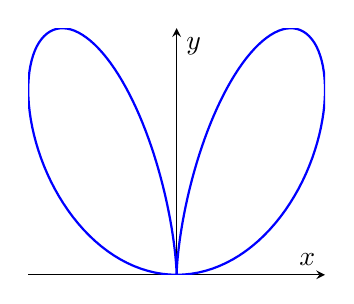
\begin{tikzpicture}
  \begin{axis}[
    ytick=\empty,
    xtick=\empty,
    scale=0.55,
    axis lines=middle,
    xlabel={$x$},
    ylabel={$y$},
  ]
    \addplot [
      domain=0:pi,
      samples=200,
      thick,
      blue,
      data cs=polarrad,
    ] {cos(deg(x))*cos(deg(x))*sin(deg(x))};
  \end{axis}
\end{tikzpicture}
\end{minipage}

\item Find the projection of the point $P(1,2,3)$ onto the plane $x+y+z=0$.
\begin{center}
\begin{tabular}{lllll}
(A) $(-1,0,1)$ &
(B) $(1,1,-2)$ &
(C) $(0,0,0)$ &
(D) $(-1,-1,2)$ &
(E) $(1,2,-3)$
\end{tabular}
\end{center}

\item Find the area of the region inside the circle $r=3\cos\theta$ and outside the cardioid $r=1+\cos\theta$.
\begin{center}
\begin{tabular}{lllll}
(A) $\pi$ &
(B) $\pi/2$ &
(C) $2\pi$ &
(D) $3\pi/4$ &
(E) $1$
\end{tabular}
\end{center}

\item Identify the quadric surface defined by the equation $2z^2 - x^2/2 - y^2 - 5 = 0$.
\begin{center}
\begin{tabular}{ll}
(A) Hyperboloid of two sheets &
(B) Hyperboloid of one sheet 
\end{tabular}

\begin{tabular}{lll}
(C) Elliptic paraboloid &
(D) Cone &
(E) Cylinder
\end{tabular}
\end{center}

\item In which direction does $f(x,y,z) = x^2 + 2y^2 - 3z$ increase most rapidly at $P(1,1,2)$?
\begin{center}
\begin{tabular}{lllll}
(A) $\langle 2, 4, -3 \rangle$ &
(B) $\langle 1, 1, -3 \rangle$ &
(C) $\langle -2, -4, 3 \rangle$ &
(D) $\langle 2, 4, 0 \rangle$ &
(E) $\langle 1, 2, -3 \rangle$
\end{tabular}
\end{center}

\item Let $w = \ln(x^2 + y^2)$ where $x = s\cos t$ and $y = s + \sin t$. Find $\dfrac{\partial w}{\partial t}$ at $(s,t) = (1, \pi/6)$.
\begin{center}
\begin{tabular}{lllll}
(A) $0$ &
(B) $1$ &
(C) $3/2$ &
(D) $\sqrt{3}/2$ &
(E) $\sqrt{3}/3$ 
\end{tabular}
\end{center}

\item Find the arc length of the curve $y = x^2/2, z = x^3/6$ from $x = 0$ to $x = 2$.
\begin{center}
\begin{tabular}{lllll}
(A) $10/3$ &
(B) $8/3$ &
(C) $4$ &
(D) $7/3$ &
(E) $3$
\end{tabular}
\end{center}

\newpage
\item A vector parallel to the tangent line of the intersection of $z = x^2 + 2y^2$ and $x^2 + (y-1)^2 = 1$ at $P(1,1,3)$ is:
\begin{center}
\begin{tabular}{lllll}
(A) $\langle 0, 2, 8 \rangle$ &
(B) $\langle 2, 4, -1 \rangle$ &
(C) $\langle 2, 0, 0 \rangle$ &
(D) $\langle 1, 1, 3 \rangle$ &
(E) $\langle 4, -2, -8 \rangle$
\end{tabular}
\end{center}

\item Which is a valid parametrization for the intersection of $z = x^2 + y^2$ and $z = 4$?
\begin{center}
\begin{tabular}{ll}
(A) $\vec{r}(t) = \langle 2\cos t, 2\sin t, 4 \rangle$ &
(B) $\vec{r}(t) = \langle \cos t, \sin t, 4 \rangle$
\end{tabular}

\begin{tabular}{lll}
(C) $\vec{r}(t) = \langle 2\cos t, 2\sin t, t \rangle$ &
(D) $\vec{r}(t) = \langle t, t^2, 4 \rangle$ &
(E) $\vec{r}(t) = \langle 2\cos t, 2\sin t, 2 \rangle$
\end{tabular}
\end{center}

\item Consider the system of equations:
\[
\begin{cases}
xu^2v + y\cos(u) = 1 \\
\ln(uv) + x^2y - u + v = 0
\end{cases}
\]
Assume that this system defines $u$ and $v$ implicitly as functions of $x$ and $y$ near the point $P(x,y,u,v) = (1,0,1,1)$.
Show that the system can be solved for $u$ and $v$ in terms of $x$ and $y$ near $P$ and find the value of $\partial u / \partial y$ at $P$.

\item \begin{enumerate}[label=\textbf{\alph*.}]
\item Consider the function
\[f(x,y) = \begin{cases}
\frac{x^2 + \sin(x)\cos(y)}{x}, & x \neq 0 \\ 
1, & x = 0 
\end{cases}.\]
Find $f_x(0,0)$ using the formal definition of the partial derivative.
    
\item Evaluate the following limit or show that it does not exist.
\[\lim_{(x,y)\to(0,0)} \frac{x^3 y^2}{x^6 + y^4}\]
\end{enumerate}

\item Find the absolute maximum and minimum values of the function
\[f(x,y) = x^2 + y^2 - 2x + 4y\]
on the closed triangular region $D$ with vertices $(0,0)$, $(4,0)$, and $(0,-4)$. Show all your work, including the analysis of the interior critical points and the boundary of the region.
\end{enumerate}

\stepcounter{section}

\newpage
\vspace*{\fill}
\begin{center}
\phantomsection
\addcontentsline{toc}{section}{\protect\numberline{\thesection}Finals}
\Huge \textbf{FINALS}
\end{center}
\vspace*{\fill}

\newpage
\stepcounter{subsection}
\phantomsection
\addcontentsline{toc}{subsection}{\protect\numberline{\thesubsection}Final - Spring 2020}

\begin{center}
\textbf{2019-2020 Spring \\MAT124-02,05 Final\\01/07/2020}
\end{center}

\begin{enumerate}[leftmargin=*,label=\textbf{\arabic*.}]
\item Find the maximum and minimum values of the function $f(x,y,z)=x-y+z$ on the sphere $x^2+y^2+z^2=100$.

\item A cylindrical tank is $4$ ft high and has an outer diameter of $2$ ft. The walls of the tank are $0.2$ in. thick. Approximate the volume of the interior of the tank assuming the tank has a top and bottom that are both also $0.2$ in. thick.

\item Let $z=f(x,y)$ be a differentiable function of $x$ and $y$, and let $x=r\cos\theta$ and $y=r\sin\theta$ for $r>0$ and $0<\theta<2\pi$. Show that
\[\left(\frac{\partial z}{\partial r}\right)^2+\frac1{r^2}\left(\frac{\partial z}{\partial\theta}\right)^2=\left(\frac{\partial z}{\partial x}\right)^2+\left(\frac{\partial z}{\partial y}\right)^2.\]

\item Reverse the order of integration in
\[\displaystyle\int_1^2\int_x^{x^3}f(x,y)\,dy\,dx+\int_2^8\int_x^8f(x,y)\,dy\,dx.\]

\item Evaluate the double integral
\[\int_1^2\int_{y^2}^{y^5}{e}^{x/y^2}\,dx\,dy.\]

\item Use a double integral to find the area of the region that lies inside the circle $r=\cos\theta$ and outside the cardioid $r=1-\cos\theta$.

\item Evaluate the volume of the solid bounded below by the cone $z=\sqrt{x^2+y^2}$ and above by the paraboloid $z=2-x^2-y^2$, by using a triple integral in cylindrical coordinates.

\item Let $T$ be the solid in the first octant bounded above by the sphere $x^2+y^2+z^2=7$ and below by the paraboloid $z=x^2+y^2$. Express (do not evalaute) the integral
\[\iiint_T\sin\left(\sqrt{x^2+y^2+z^2}\right)\,dV\]

in spherical coordinates.
\end{enumerate}

\newpage
\stepcounter{subsection}
\phantomsection
\addcontentsline{toc}{subsection}{\protect\numberline{\thesubsection}Resit - Spring 2020}
\begin{center}
\textbf{2019-2020 Spring\\MAT124 Resit\\01/07/2020}
\end{center}

\begin{enumerate}[leftmargin=*,label=\textbf{\arabic*.}]
\item The temperature $T$ at the point $(x,y,z)$ in a region of space is given by the formula $T=100-xy-xz-yz$. Find the lowest temperature on the plane $x+y+z=10$.

\item Show that if $z=f(r, \theta)$, where $r$ and $\theta$ are defined as functions of $x$ and $y$ by the equations $x=r\cos\theta$ and $y=r\sin\theta$, then the equation $\displaystyle\frac{\partial^2z}{\partial x^2}+\frac{\partial ^2z}{\partial y^2} = 0$ becomes
\[\frac{\partial^2z}{\partial r^2}+\frac{1}{r^2}\frac{\partial^2z}{\partial\theta^2}+\frac{1}{r}\frac{\partial z}{\partial r}=0\:.\]

\item Evaluate the integral $\displaystyle \int_0^1\int_{\sqrt y}^1 \sqrt{1-x^3}\,dx\,dy$.

\item Evaluate
\[\int_2^4\int_2^y\,dx\,dy + \int_4^8\int_2^{16/y}\,dx\,dy\]

by reversing the order of integration.

\item Use a double integral to find the area inside the circle $r=\cos\theta$ and outside the cardioid $r=1-\cos\theta$.

\item Use polar coordinates to evaluate the double integral
\[\iint_D\sin\left(x^2+y^2\right)\,dA,\]

where $D$ is the region bounded by the circles $x^2+y^2=1$ and $x^2+y^2=4$ and the lines $y=0$, $x=\sqrt3 y$.

\item Using cylindrical coordinates, evaluate
\[\iiint_D\frac{dV}{x^2+y^2+z^2},\]

where $D$ is the solid region bounded below by the paraboloid $2z=x^2+y^2$ and above by the sphere $x^2+y^2+z^2=8$.

\item Using spherical coordinates, evaluate the triple integral
\[\iiint_D\sqrt{x^2+y^2+z^2}\,dV,\]

where $D$ is the portion of the solid sphere $x^2+y^2+z^2\leq1$ that lies in the first octant.
\end{enumerate}

\newpage
\stepcounter{subsection}
\phantomsection
\addcontentsline{toc}{subsection}{\protect\numberline{\thesubsection}Final - Summer 2020}
\begin{center}
\textbf{2019-2020 Summer\\MAT124 Final\\28/08/2020}
\end{center}

\begin{enumerate}[leftmargin=*,label=\textbf{\arabic*.}]
\item Find the maximum and minimum values of the function $f(x,y)=x^2+y^2-3y$ on the closed disk $x^2+y^2\leq4$.

\item The velocity of a particle moving in space is
\[\mathbf{V}(t)=\ln t\,\mathbf{i} +\sin t\,\mathbf{j}+ t^3\,\mathbf{k}\]

Find the particle's position as a function of $t$ if the position at time $t=1$ is \linebreak $\mathbf{R}(1)=2\mathbf{i}+\mathbf{j}-\mathbf{k}$.
\item Evaluate the integral $\displaystyle \int_0^1\int_{y^2}^1 y^3\cos x^3\,dx\,dy$.

\item Let $R$ be the region lying inside $r=1$ and outside $r=1+\cos\theta$.

\begin{enumerate}[leftmargin=*,label=\textbf{\alph*.}]
\item Sketch the graph of the region $R$.
\item Set up (but do not evaluate) a double integral in polar coordinates for the area of the region $R$.
\end{enumerate}

\item Let $S$ be the surface of the portion of the cone $z^2=x^2+y^2$ that is contained in the cylinder $x^2+y^2=9$.

\begin{enumerate}[leftmargin=*,label=\textbf{\alph*.}]
\item Sketch the graph of $S$.
\item Evaluate the surface area using polar coordinates.
\end{enumerate}

\item Let $S$ be the region bounded by the paraboloids $z=8-x^2-y^2$ and $z=x^2+y^2$.

\begin{enumerate}[leftmargin=*,label=\textbf{\alph*.}]
\item Using the spherical coordinates, set up (but do not evaluate) an integral for the volume of the solid $S$.
\item Using the cylindrical coordinates, set up (but do not evaluate) an integral for the volume of the solid $S$.
\end{enumerate}
\end{enumerate}

\newpage
\stepcounter{subsection}
\phantomsection
\addcontentsline{toc}{subsection}{\protect\numberline{\thesubsection}Final - Spring 2021}

\begin{center}
\textbf{2020-2021 Spring \\MAT124 Final\\09/06/2021}
\end{center}

\begin{enumerate}[leftmargin=*,label=\textbf{\arabic*.}]
\item Sketch the region corresponding to the double integral
\[\int_{-1}^2\int_{x^2}^{x+2}\,dy\,dx\]
and reverse the order of integration.

\item Find the volume of the solid bounded above by the cone $z=\sqrt{x^2+y^2}$ and below by the circular region $x^2+y^2\leq4$ in the $xy$-plane.

\item Let $R$ be the region lying outside $r=1$ and inside $r=1+\cos\theta$.
\begin{enumerate}[leftmargin=*,label=\textbf{\alph*.}]
\item Sketch the graph of the region $R$.
\item Set up (but do not evaluate) a double integral in polar coordinates for the area of the region $R$.
\end{enumerate}

\item Let $S$ be the portion of the surface $z=y^2$ that lies over the rectangular region in the $xy$-plane with the vertices $(0,0,0), (0,1,0), (1,1,0)$ and $(1,0,0)$.
\begin{enumerate}[leftmargin=*,label=\textbf{\alph*.}]
\item Sketch the graph of $S$.
\item Evaluate the surface area.
\end{enumerate}

\item Evaluate $\displaystyle \iiint_E z\,dV$, where $E$ is the region bounded below by $x^2+y^2+z^2=4$ and above by $x^2+y^2+z^2=9$.

\item Let $S$ be the region bounded above by the paraboloid $z=1-x^2-y^2$ and below by the $xy$-plane.
\begin{enumerate}[leftmargin=*,label=\textbf{\alph*.}]
\item Using the spherical coordinates, set up (but do not evaluate) an integral for the volume of the solid $S$.
\item Using the cylindrical coordinates, set up (but do not evaluate) an integral for the volume of the solid $S$.
\end{enumerate}
\end{enumerate}

\newpage
\stepcounter{subsection}
\phantomsection
\addcontentsline{toc}{subsection}{\protect\numberline{\thesubsection}Final - Spring 2022}

\begin{center}
\textbf{2021-2022 Spring \\MAT124 Final\\23/05/2022}
\end{center}

\begin{enumerate}[leftmargin=*,label=\textbf{\arabic*.}]
\item Find the largest and smallest values of $f(x,y) = x^2+y^2$ subject to the constraint $x+y=1$ with $x\geq0$ and $y\geq0$.

\item Sketch the region corresponding to the double integral
\[\int_0^{\frac{-1+\sqrt5}{2}}\int_{\sqrt{y}}^{\sqrt{1-y^2}}\,dx\,dy\]
and reverse the order of integration. Do not evaluate the integral!

\item Sketch the region inside the circle $r=1$ and outside the cardioid $r=1+\sin\theta$ and then, using a double integral, find the area of the region.

\item Using a double integral, find the volume of the solid bounded above by the sphere $x^2+y^2+z^2 = 16$ and below by the circular region $x^2+y^2\leq2$ in the $xy$-plane.

\item Let us consider the frustum of the cone $z=\sqrt{x^2+y^2}$ between the planes $z=1$ and $z=2$.

\begin{enumerate}[leftmargin=*,label=\textbf{\alph*.}]
\item Sketch the graph of the frustum.
\item Find the surface area of the frustum.
\end{enumerate}

\item Let $S$ be the region in the cylinder $x^2+y^2 = 1$ bounded above by the plane $z=6$ and below by the paraboloid $z=1-x^2-y^2$.

\begin{enumerate}[leftmargin=*,label=\textbf{\alph*.}]
\item Using the spherical coordinates, set up (but do not evaluate!) an integral for the volume of the solid $S$.
\item Using the cylindrical coordinates, find the volume of the solid $S$.
\end{enumerate}
\end{enumerate}


\newpage
\stepcounter{subsection}
\phantomsection
\addcontentsline{toc}{subsection}{\protect\numberline{\thesubsection}Final - Spring 2023}
\begin{center}
\textbf{2022-2023 Spring \\MAT124 Final\\12/06/2023}
\end{center}

\begin{enumerate}[leftmargin=*,label=\textbf{\arabic*.}]
\item Maximize the function $f(x,y)=xy^2z$ on the sphere $x^2+y^2+z^2 = 4$.

\item Sketch the region corresponding to the double integral
\[\int_0^1\int_{x^{1/4}}^1\,{e}^{y^5}dy\,dx\]
and evaluate it.

\item Sketch the region $R$ inside the cardioid $r=1+\cos\theta$ and outside the limaçon $r=2-\cos\theta$, and set up the polar double integral corresponding to the area of the region $R$.

\item Using a double integral, find the volume of the solid bounded above by the elliptic paraboloid $z=4-x^2-y^2$ and below by the circular region $x^2+y^2\leq2$ in the $xy$-plane where $x\geq0$ and $y\geq0$.

\item Let us consider the frustum of the cone $z=\sqrt{x^2+y^2}$ between the planes $z=1$ and $z=2$.

\begin{enumerate}[leftmargin=*,label=\textbf{\alph*.}]
\item Sketch the graph of the frustum.
\item Find the surface area of the frustum.
\end{enumerate}

\item Let $S$ be the region in the cylinder $x^2+y^2 = 1$ bounded above by the plane $z=4$ and below by the sphere $x^2+y^2+z^2=1$.
\begin{enumerate}[leftmargin=*,label=\textbf{\alph*.}]
\item Using the spherical coordinates, set up (but do not evaluate!) an integral for the volume of the solid $S$.
\item Using the cylindrical coordinates, find the volume of the solid $S$.
\end{enumerate}
\end{enumerate}
\newpage
\stepcounter{subsection}
\phantomsection
\addcontentsline{toc}{subsection}{\protect\numberline{\thesubsection}Makeup - Spring 2023}
\begin{center}
\textbf{2022-2023 Spring \\MAT124 Makeup\\12/06/2023}
\end{center}

\begin{enumerate}[leftmargin=*,label=\textbf{\arabic*.}]
\item Find the absolute extrema of $f(x,y) = 2x^2-y^2$ on the closed, bounded set $x^2+y^2\leq1$ in the plane.

\item Sketch the region corresponding to the double integral
\[\int_{-3}^2\int_{x^2}^{6-x}dy\,dx\]
and evaluate the integral by writing the equivalent integral with the order of integration reversed.

\item Using a double integral, find the area enclosed by the upper half of the cardioid $r=1+\sin\theta$.

\item Sketch the region $R$ bounded above by the elliptic paraboloid $z=2-x^2-y^2$ and below by the paraboloid $z=x^2+y^2$. Using a double integral find the volume of $R$.

\item Find the surface area of the portion of the sphere $x^2+y^2+z^2=4$ that is above the $xy$-plane and within the cylinder $x^2+y^2=1$.

\item \begin{enumerate}[leftmargin=*,label=\textbf{\alph*.}]
\item Sketch the graph of the region $R$ bounded above by the paraboloid $z=4-x^2-y^2$ and below by the plane $z=4-2x$.

\item Evaluate the volume of $R$.
\end{enumerate}
\end{enumerate}
\newpage
\stepcounter{subsection}
\phantomsection
\addcontentsline{toc}{subsection}{\protect\numberline{\thesubsection}Final - Spring 2024}
\begin{center}
\textbf{2023-2024 Spring \\MAT124 Final\\04/06/2024}
\end{center}

\begin{enumerate}[leftmargin=*,label=\textbf{\arabic*.}]
\item Using Lagrange multipliers, find the closest point of the plane $x+z+1=0$ to the point $(1,2,0)$.

\item Sketch the region and reverse the order of the double integral
\[\int_0^1\int_0^{x^2/2}dy\,dx+\int_1^{\sqrt2}\int_{x^2-1}^{x^2/2}dy\,dx\]

\item Sketch the region and use a double integral in polar coordinates to find the area inside the cardioid $r=1-\cos\theta$ outside the circle $r=1$.

\item Sketch the region and use a double integral to find the volume of the solid bounded above by the plane $x=z$ and below in the $xy$-plane by the part of the disk $x^2+y^2\leq4$ in the fourth quadrant.

\item Find the surface area of the portion of the paraboloid $z=25-x^2-y^2$ that lies above the $xy$-plane.

\item Using the change of variables $u=x-y$ and $v=x+y$, evaluate the integral
\[\iint_{\mathcal{R}}(x-y)\sin\left(x^2-y^2\right)\,dy\,dx\]
where $\mathcal{R}$ is the region bounded by the lines $x+y=1$ and $x+y=3$ and the curves $x^2-y^2=-1$ and $x^2-y^2=1$.

\item Let $R$ be the solid region bounded by the cone $z=\sqrt{3x^2+3y^2}$ and above by the sphere $x^2+y^2+z^2=9$. Let
\[{I}=\iiint_R\left(x^2+y^2\right)\,dV\]

\begin{enumerate}[leftmargin=*,label=\textbf{\alph*.}]
\item Express (but do not evaluate) ${I}$ as a triple integral in spherical coordinates.
\item Express (but do not evaluate) ${I}$ as a triple integral in cylindrical coordinates.
\end{enumerate}
\end{enumerate}
\newpage
\stepcounter{subsection}
\phantomsection
\addcontentsline{toc}{subsection}{\protect\numberline{\thesubsection}Final - Fall 2024}
\begin{center}
\textbf{2023-2024 Fall \\MAT124 Final\\11/01/2024}
\end{center}

\begin{enumerate}[leftmargin=*,label=\textbf{\arabic*.}]
\item \begin{enumerate}[leftmargin=*,label=\textbf{\alph*.}]
\item Find the critical points of the function
\[f(x,y)={e}^y\left(y^2-x^2\right)\]
and classify them.
\item Find the maximum and minimum values of the function
\[f(x,y,z)=xyz^2\]
by using Lagrange multipliers on the region $D:x+y+z=1,\:x\geq0,\:y\geq0,\:z\geq0$.
\end{enumerate}

\item \begin{enumerate}[leftmargin=*,label=\textbf{\alph*.}]
\item Sketch the domain of integration, and rewrite the integral by changing the order of integration.
\[\int_0^1\int_{\sqrt{1-y}}^1f(x,y)\,dx\,dy+\int_1^3\int_{\textstyle\frac{y-1}2}^1f(x,y)\,dx\,dy\]

\item Evaluate the integral
\[\iint_R\sqrt{x^2+y^2}\,dA\]
where $R$ is the region bounded by the line $x=1$ on the left and by the circle $x^2+y^2=2$ on the right.
\end{enumerate}

\item Convert
\[\int_0^{2\pi}\int_0^{\sqrt2}\int_r^{\sqrt{4-r^2}}3\,dz\,r\,dr\,d\theta,\quad r\geq0\]

\begin{enumerate}[leftmargin=*,label=\textbf{\alph*.}]
\item to rectangular coordinates with the order of integration $dz\,dx\,dy$.
\item to spherical coordinates.
\end{enumerate}

\item \begin{enumerate}[leftmargin=*,label=\textbf{\alph*.}]
\item Is $\mathbf{F}(x,y)=2xy\cos\left(x^2y\right)\mathbf{i}-x^2\cos\left(x^2y\right)\mathbf{j}$ conservative? Why?
\item Show that
\begin{align*}\mathbf{F}(x,y,z)=&\left(y^2\cos\left(xy^2\right)+yz^2\right)\mathbf{i}\\&+\left(2xy\cos\left(xy^2\right)+xz^2+z{e}^{yz}\right)\mathbf{j}+\left(2xyz+y{e}^{yz}+2z\right)\mathbf{k}\end{align*}
is conservative.
\item Find its potential function.
\end{enumerate}
\end{enumerate}

\newpage
\stepcounter{subsection}
\phantomsection
\addcontentsline{toc}{subsection}{\protect\numberline{\thesubsection}Resit - Fall 2024}

\begin{center}
\textbf{2023-2024 Fall \\MAT124 Resit\\29/01/2024}
\end{center}

\begin{enumerate}[leftmargin=*,label=\textbf{\arabic*.}]
\item \begin{enumerate}[leftmargin=*,label=\textbf{\alph*.}]
\item Find the critical points of the function
\[f(x,y)=4x^3-6xy+y^2+2y\]
and classify them.

\item Find the maximum and minimum values of the function
\[f(x,y,z)=x+y+z\]

by using Lagrange multipliers on the ellipsoid $x^2+4y^2+9z^2=1764$.
\end{enumerate}

\item \begin{enumerate}[leftmargin=*,label=\textbf{\alph*.}]
\item Sketch the domain of integration and rewrite the integral by changing the order of integration.

\[\int_0^1\int_0^{x\sqrt3}{e}^{-x^2-y^2}\,dy\,dx+\int_1^2\int_0^{\sqrt{4-x^2}}{e}^{-x^2-y^2}\,dy\,dx\]

\item Evaluate the integral
\[\iint_R\frac{xy}{1+x^4}\,dA\]
where $R$ is the triangle with vertices $(0,0),\:(1,0)$ and $(1,1)$.

\end{enumerate}

\item The following integral gives the volume of the region that lies inside the sphere $x^2+y^2+z^2=4$ and between the planes $z=0$ and $z=1$.
\[V=4\int_0^{\pi/2}\int_0^{\sqrt3}\int_0^1r\,dz\,dr\,d\theta+4\int_0^{\pi/2}\int_{\sqrt3}^2\int_0^{\sqrt{4-r^2}}r\,dz\,dr\,d\theta\]

\begin{enumerate}[leftmargin=*,label=\textbf{\alph*.}]
\item Write the integral in rectangular coordinates with the order of integration $dz\,dy\,dx$.

\item Write the integral in spherical coordinates.
\end{enumerate}

\item \begin{enumerate}[leftmargin=*,label=\textbf{\alph*.}]
\item Is $\mathbf{F}(x,y)=2xy\sin\left(x^2y\right)\mathbf{i}-x^2\sin\left(x^2y\right)\mathbf{j}$ conservative? Why?
\item Show that
\[\mathbf{F}(x,y,z)=\left(2x+y^2+z\cos x\right)\mathbf{i}+\left(2xy+{e}^z\right)\mathbf{j}+\left(1+y{e}^z+\sin x\right)\mathbf{k}\]
is conservative.
\item Find its potential function.
\end{enumerate}

\newpage

\item $\mathbf{F}(x,y,z)=\left(2x+y^2+z\cos x\right)\mathbf{i}+\left(2xy+{e}^z\right)\mathbf{j}+\left(1+y{e}^z+\sin x\right)\mathbf{k}$

\begin{enumerate}[leftmargin=*,label=\textbf{\alph*.}]
\item Let $C $ be the curve of intersection of the cone $z^2=4x^2+9y^2$ and the plane $z=1+x+2y$, and let $D$ be the part of the curve $C$ that lies in the first octant $x\geq0,\:y\geq0,\:z\geq0$ from $(1,0,2)$ to $(0,1,3)$. Evaluate $\int_D\mathbf{F}\cdot d\mathbf{r}$.

\item Let $C$ be the curve of intersection of $x^2+y^2=1$ and $z=40$. Evaluate $\int_C\mathbf{F}\cdot d\mathbf{r}$.
\end{enumerate}

\item Evaluate

\[\oint_C\left(x^3\sin\left(\sqrt{x^2+4}\right)-x{e}^{x+2y}\right)\,dx + \left(\cos\left(y^3+y\right)-4y{e}^{x+2y}\right)\,dy\]

where $C$ is the counterclockwise boundary of the parallelogram with vertices $(2,0)$, $(0,-1)$, $(-2,0)$, and $(0,1)$.
\end{enumerate}

\newpage
\stepcounter{subsection}
\phantomsection
\addcontentsline{toc}{subsection}{\protect\numberline{\thesubsection}Makeup - Spring 2024}
\begin{center}
\textbf{2023-2024 Spring \\MAT124 Makeup\\27/06/2024}
\end{center}

\begin{enumerate}[leftmargin=*,label=\textbf{\arabic*.}]
\item Find the maximum and minimum values of $f(x,y,z)=x-y+z$ on the sphere $x^2+y^2+z^2=100$.

\item Sketch the region and reverse the order of the double integral
\[\int_0^{\bcancel4\:3}\int_{y/3}^{\sqrt{4-y}}dx\,dy\]

\item Using a polar double integral, find the volume of the sphere with radius $4$.

\item Find the surface area of the portion of the paraboloid $z=x^2+y^2$ that lies in the cylinder $x^2+y^2=1$.

\item Using the change of variables, evaluate the area of the ellipse $\displaystyle\frac{x^2}{16}+\frac{y^2}{25}=1$.

\item Let $R$ be the solid region bounded below by the cone $z=\sqrt{3x^2+3y^2}$ and above by the sphere $x^2+y^2+z^2=9$. Let
\[{I}=\iiint_R(x^2+y^2)\,dV.\]

\begin{enumerate}[leftmargin=*,label=\textbf{\alph*.}]
\item Express (but do not evaluate) ${I}$ as a triple integral in spherical coordinates.
\item Express (but do not evaluate) ${I}$ as a triple integral in cylindrical coordinates.
\end{enumerate}
\end{enumerate}

\newpage
\stepcounter{subsection}
\phantomsection
\addcontentsline{toc}{subsection}{\protect\numberline{\thesubsection}Final - Spring 2025}

\begin{center}
\textbf{2024-2025 Spring \\MAT124 Final\\18/06/2025}
\end{center}

\begin{enumerate}[leftmargin=*,label=\textbf{\arabic*.}]
\item Let $f(x,y)=6-x^2-y^2$. Find the tangent plane and normal line equations (symmetric or parametric equations) of the graph of $f$ at the point $P(1,2,1)$.

\item Find all critical points of the given function $f(x,y)=x^3+y^3-3xy+2$ and classify them (i.e., determine whether each critical point corresponds to a local maximum, local minimum, or saddle point).

\item Find the maximum and minimum of the function $f(x,y)=81x^2+y^2$ subject to the given constraint $4x^2+y^2=9$ using Lagrange multipliers.

\item The equation $z^3-zy^2+yx=3$ defines $z$ implicitly as a function of $x$ and $y$. It is given that $z=2$ when $(x,y)=(-3,1)$. Evaluate $\displaystyle\frac{\partial z}{\partial x}$ and $\displaystyle\frac{\partial z}{\partial y}$ at $(-3,1)$.

\item \begin{enumerate}[leftmargin=*,label=\textbf{\alph*.}]
\item Reverse the order of integration and evaluate the double integral.
\[\int_0^{\sqrt2}\int_0^{2-x^2}x{e}^{x^2}\,dy\,dx\]
 
\item Evaluate the double integral
\[\iint_R \frac{2xy}{x^2+y^2}\,dA\]
where the region $R = \{(x,y): x\geq0,\:y\geq0,\:z\geq0,\:x^2+y^2\leq a^2\}$
\end{enumerate}

\item \begin{enumerate}[leftmargin=*,label=\textbf{\alph*.}]
\item Convert the triple integral into cylindrical coordinates. Do not evaluate the integral.
\[\int_{-1}^1\int_0^{\sqrt{1-y^2}}\int_{x^2+y^2}^{\sqrt{x^2+y^2}}xyz\,dz\,dx\,dy\]

\item Use a triple integral in spherical coordinates in order to find the volume of the sphere centered at $(0,0,0)$ with radius $3$.
\end{enumerate}

\item \begin{enumerate}[leftmargin=*,label=\textbf{\alph*.}]
\item Determine whether the vector field $\mathbf{F}(x,y,z)=y\,\mathbf{i}+x\,\mathbf{j}+z^2\,\mathbf{k}$ is conservative and find a potential if it is conservative.

\item Evaluate the line integral $\int_C\mathbf{F}\cdot d\mathbf{r}$ for the vector field $\mathbf{F}(x,y,z)=z\,\mathbf{i}-y\,\mathbf{j}+2x\,\mathbf{k}$ along the curve $x=t,\:y=t^2\:z=t^3$ from $(0,0,0)$ to $(1,1,1)$.
\end{enumerate}
\end{enumerate}

\newpage
\stepcounter{subsection}
\phantomsection
\addcontentsline{toc}{subsection}{\protect\numberline{\thesubsection}Final - Spring 2026}

\begin{center}
\textbf{2025-2026 Spring \\MAT124 Final\\08/06/2026}
\end{center}

\begin{enumerate}[leftmargin=*,label=\textbf{\arabic*.}]
\item Use the method of Lagrange multipliers to find the absolute maximum and absolute minimum values of the function $f(x, y, z) = x^2 + 2y - z^2$ subject to the constraint $2x^2 + y^2 + z^2 = 4$.

\item Consider the vector field
\[\mathbf{F}(x, y, z) = (2xe^y + z \cos(xz))\mathbf{i} + (x^2 e^y - \sin(y))\mathbf{j} + (x \cos(xz) + 2z)\mathbf{k}.\]
\begin{enumerate}[leftmargin=*,label=\textbf{\alph*.}]
\item Show that $\mathbf{F}$ is a conservative vector field by verifying the cross-partial derivative conditions.
\item Find a potential function $\phi(x, y, z)$ such that $\mathbf{F} = \nabla\phi$.
\item Evaluate the line integral $\int_C \mathbf{F} \cdot d\mathbf{r}$, where $C$ is the path given by \linebreak $\mathbf{r}(t) = \left\langle t, t(1-t), \frac{\pi}{2}t^3 \right\rangle$ for $0 \le t \le 1$.
\end{enumerate}

\item Let $C$ be the upper half of the circle $x^2 + y^2 = 9$, oriented from $(3, 0)$ to $(-3, 0)$. Evaluate the line integral
\[\int_C \left(y^2 + \sin(x^3)\right) dx + \left(3xy + e^{y^2}\right) dy.\]
\textit{Hint: The curve $C$ is not closed. Consider adding a line segment to form a closed loop and use Green's Theorem.}

\item Answer the following questions. For multiple choice questions, mark the correct option. For others, write your answer in the box provided. No partial credits will be given.

\begin{enumerate}[leftmargin=*, label=\textbf{\arabic{enumi}.\arabic*.}]
\item Consider the iterated double integral $\int_{-8}^8 \int_{x^{2/3}}^4 f(x, y)\,dy\,dx$. Reverse the order of integration and write the new limits in the boxes below:
\[\int_{\boxed{\phantom{\rule{1.5cm}{0.5cm}}}}^{\boxed{\phantom{\rule{1.5cm}{0.5cm}}}} \int_{\boxed{\phantom{\rule{1.5cm}{0.5cm}}}}^{\boxed{\phantom{\rule{1.5cm}{0.5cm}}}} f(x,y)\,dx\,dy\]

\item Let $E$ be the solid region bounded above by the paraboloid $z = x^2 + y^2$, below by the $xy$-plane ($z = 0$), and enclosed by the elliptic cylinder $x^2 + 4y^2 = 4$. What is the volume of the region $E$? \\
\textit{(Hint: Use a modified coordinate system such as $x = 2r \cos\theta$ and $y = r \sin\theta$ to simplify the region).}

\begin{enumerate*}[label=(\Alph*), itemjoin=\hspace{1.5cm}]
\item $\dfrac{3\pi}{2}$
\item $2\pi$
\item $\dfrac{5\pi}{2}$
\item $3\pi$
\item $4\pi$
\end{enumerate*}

\newpage
\item Consider the vector field $\mathbf{F}(x, y) = \left\langle y^2, -\frac{2}{x-2} \right\rangle$ representing the velocity field of a steady fluid flow. Imagine placing a tiny paddle wheel into this fluid. The paddle wheel will rotate counter-clockwise if the scalar curl of the field is positive, and clockwise if it is negative. In which of the following regions above the $x$-axis ($y > 0$) will the paddle wheel definitely rotate in a counter-clockwise direction?

\begin{enumerate}
    \item[(A)] $0 < y < \dfrac{1}{(x-2)^2}$
    \item[(B)] $y^2 > \dfrac{2}{x-2}$
    \item[(C)] $y^2 < \dfrac{2}{x-2}$
    \item[(D)] $y > \dfrac{1}{(x-2)^2}$
    \item[(E)] Everywhere above the $x$-axis.
\end{enumerate}

\item Let $D$ be the region in the $xy$-plane bounded by the lines $y = x$, $y = x - 2$, $y = -x$, and $y = -x + 3$. Using an appropriate change of variables, evaluate the double integral:
\[\iint_D (x + y) e^{x^2 - y^2}\,dA\]

\begin{enumerate*}[label=(\Alph*), itemjoin=\hspace{0.7cm}]
    \item $\dfrac{1}{2}(e^6 - 1)$
    \item $\dfrac{1}{4}(e^6 - 7)$
    \item $e^6 - 7$
    \item $\dfrac{3}{2}(e^4 - 1)$
    \item $2(e^6 - 3)$
\end{enumerate*}

\item Which of the following curves represents a field line (integral curve) for the vector field $\mathbf{F}(x, y) = y\mathbf{i} + x\mathbf{j}$? (where $C$ is a constant)

\begin{enumerate*}[label=(\Alph*), itemjoin=\hspace{0.5cm}]
\item $x^2 + y^2 = C$
\item $y = Cx$
\item $y = C e^x$
\item $x^2 - y^2 = C$
\item $xy = C$
\end{enumerate*}

\item Calculate the outward flux of the vector field $\mathbf{F}(x, y, z) = x^3\mathbf{i} + y^3\mathbf{j} + z^3\mathbf{k}$ across the surface of the unit sphere $x^2 + y^2 + z^2 = 1$.

\begin{enumerate*}[label=(\Alph*), itemjoin=\hspace{1.5cm}]
\item $\dfrac{4\pi}{5}$
\item $\dfrac{8\pi}{5}$
\item $\dfrac{12\pi}{5}$
\item $4\pi$
\item $12\pi$
\end{enumerate*}

\item Consider the following two vector fields in $\mathbb{R}^3$:
\[\mathbf{F}_1 = \langle -y, x, 0 \rangle \quad \text{and} \quad \mathbf{F}_2 = \langle x, y, z \rangle\]
How can these fields be classified?

\begin{enumerate}
    \item[(A)] Both are solenoidal.
    \item[(B)] Both are irrotational.
    \item[(C)] $\mathbf{F}_1$ is solenoidal, $\mathbf{F}_2$ is irrotational.
    \item[(D)] $\mathbf{F}_1$ is irrotational, $\mathbf{F}_2$ is solenoidal.
    \item[(E)] Neither field is solenoidal nor irrotational.
\end{enumerate}

\item The vector field $\mathbf{F}(x, y, z) = 2y\mathbf{i} + z\mathbf{j} + 0\mathbf{k}$ is solenoidal. Find a vector potential $\mathbf{A}$ such that $\nabla \times \mathbf{A} = \mathbf{F}$. Assume the $x$-component of the vector potential is zero. Write the remaining components.

\end{enumerate}
\end{enumerate}

\newpage
\renewcommand{\headrulewidth}{0pt}
\fancyhead[L]{}
\fancyhead[R]{}

\stepcounter{section}
\vspace*{\fill}
\begin{center}
\phantomsection
\addcontentsline{toc}{section}{\protect\numberline{\thesection}Midterm Solutions}
\Huge \textbf{MIDTERM SOLUTIONS}
\end{center}
\vspace*{\fill}

\newpage
\renewcommand{\headrulewidth}{1pt}
\fancyhead[L]{\textit{Hacettepe MAT124 Exam Solutions Version 2}}

\stepcounter{subsection}
\phantomsection
\addcontentsline{toc}{subsection}{\protect\numberline{\thesubsection}Midterm I - Spring 2012 Solutions}

\fancyhead[R]{\textit{2011-2012 Spring Midterm I}}

%(Last update: 19/8/25 (19th of August) 22:35)

\begin{enumerate}[leftmargin=*,label=\textbf{\arabic*.}]
\item

\begin{enumerate}[leftmargin=*,label=\textbf{\alph*.}]
\item \leavevmode

\vspace{-1em}
\begin{center}
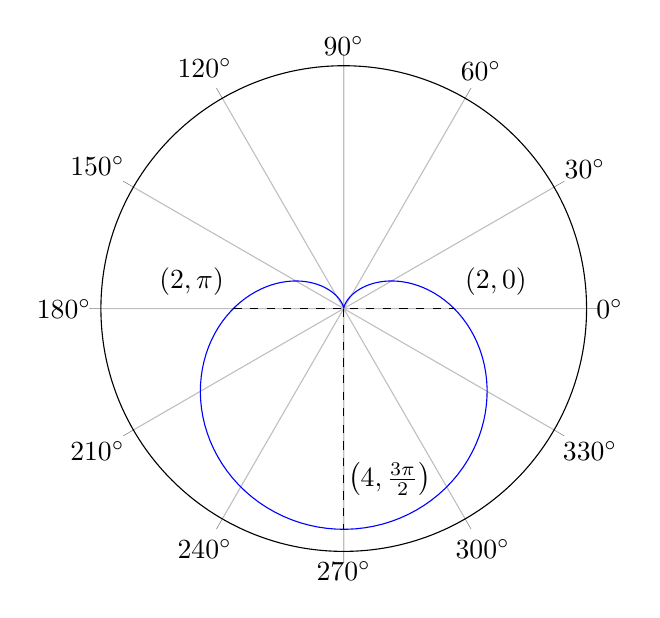
\begin{tikzpicture}
  \begin{polaraxis}[ytick=\empty, axis y line=none, xticklabel=$\pgfmathprintnumber{\tick}^\circ$, scale=0.9]
    \addplot [
      domain=0:2*pi,
      samples=150,
      blue,
      data cs=polarrad,
    ] {2-2*sin(deg(x))};

    \draw[dashed] (axis cs: 0,-2) -- (axis cs: 0,2);
    \node at (axis cs: -10,-2.8) {$(2,\pi)$};
    \node at (axis cs: 10,2.8) {$(2,0)$};
    \node at (axis cs: 285,3.2) {$\left(4,\frac{3\pi}2\right)$};
    \draw[dashed] (axis cs: 0,0) -- (axis cs: 270,4);

  \end{polaraxis}
\end{tikzpicture}
\end{center}

\item\leavevmode

\vspace{-3em}
\begin{align*}A&=\frac12\int_a^br^2\,d\theta=\frac12\int_0^{2\pi}\left(2-2\sin\theta\right)^2\,d\theta=\frac12\int_0^{2\pi}\left(4-8\sin\theta+4\sin^2\theta\right)\,d\theta\\[1em]&=\frac12\int_0^{2\pi}\left(4-8\sin\theta+4\sin^2\theta\right)\,d\theta=\int_0^{2\pi}\left(2-4\sin\theta+1-\cos2\theta\right)\,d\theta\\[1em]&=\left[2\theta+4\cos\theta+\theta-\frac12\sin2\theta\right]_0^{2\pi}=\left[\left(4\pi+4+2\pi\right)-(4)\right]=\boxed{6\pi}\end{align*}

\item The slope of the tangent line in terms of $r$ and $\theta$ is
\[\left.\frac{dy}{dx}\right|_{(r,\theta)}=\frac{f'(\theta)\cdot\sin\theta+f(\theta)\cdot\cos\theta}{f'(\theta)\cdot\cos\theta-f(\theta)\cdot\sin\theta}\]

\[f(\theta)=2-2\sin\theta, \quad f'(\theta)=-2\cos\theta\]

\[\frac{dy}{dx}=\frac{-2\cos\theta\cdot\sin\theta+(2-2\sin\theta)\cdot\cos\theta}{-2\cos\theta\cdot\cos\theta-(2-2\sin\theta)\cdot\sin\theta}=\frac{-2\sin2\theta+2\cos\theta}{-\sin2\theta-2\sin\theta+2\sin^2\theta}\]

\[\left.\frac{dy}{dx}\right|_{\left(2-\sqrt2,\:\pi/4\right)}=\frac{-2+\sqrt2}{-\sqrt2}=\sqrt2-1\]

The tangent vectors to the curve at $\theta=\dfrac\pi4$ are
\[\boxed{\left\langle k,\:k\left(\sqrt2-1\right)\right\rangle,\quad k\in\mathbb{R}}\]
\end{enumerate}

\item \begin{enumerate}[leftmargin=*,label=\textbf{\alph*.}]
\item Choose three arbitrary points and determine the parallel vector of each of the two line segments that connect the points.

\[\overrightarrow{AB}=\left\langle-1-0,\:0-(-1),\:1-1\right\rangle=\left\langle-1,1,0\right\rangle\]
\[\overrightarrow{AC}=\left\langle1-0,\:0-(-1),\:2-1\right\rangle=\left\langle1,1,1\right\rangle\]

The cross product of these vectors gives us the normal vector of the plane.
\begin{align*}\mathbf{n}&=\left|\begin{array}{ccc}
\mathbf{i}&\mathbf{j}&\mathbf{k}\\
-1&1&0\\
1&1&1
\end{array}\right|=\mathbf{i}\left|\begin{array}{cc}
1&0\\1&1
\end{array}\right|-\mathbf{j}\left|\begin{array}{cc}
-1&0\\1&1
\end{array}\right|+\mathbf{k}\left|\begin{array}{cc}
-1&1\\1&1
\end{array}\right|\\[1em]&=(1\cdot1-0\cdot1)\mathbf{i}-(-1\cdot1-0\cdot1)\mathbf{j}+(-1\cdot1-1\cdot1)\mathbf{k}=\mathbf i+\mathbf j-2\mathbf k\end{align*}

The plane has the equation $\mathbf n\cdot\overrightarrow{PP_0}=0$. Since $C(1,0,2)$ is on the plane, the equation of the plane is
\[\boxed{1(x-1)+1(y-0)-2(z-2)=0\implies x+y-2z+3=0}\]

\item Let $P$ be a point on a plane, then the distance from any point $R$ to the plane is the length of the vector projection of $\overrightarrow{PR}$ onto $\mathbf n$. That is,
\[d=\left|\overrightarrow{PR}\cdot\frac{\mathbf n}{|\mathbf n|}\right|\]

The distance from $D$ to the plane passing through $A, B, C$ can be calculated using
\[d=\left|\overrightarrow{AD}\cdot\frac{\mathbf n}{|\mathbf n|}\right|=\left|\left\langle0-0,0-(-1),1-1\right\rangle\cdot\frac{\left\langle1,1,-2\right\rangle}{\sqrt{1^2+1^2+(-2)^2}}\right|=\boxed{\frac1{\sqrt6}}\]

\item We have
\[\mathbf{v}=\overrightarrow{BD}=\left\langle0-(-1),0-0,1-1\right\rangle=\left\langle1,0,0\right\rangle\]

The parametric equations for a line that passes through the point $P_0(x_0,y_0,z_0)$ is given by
\[\left.\begin{array}{c}
x=x_0+v_1t\\[1em]
y=y_0+v_2t\\[1em]
z=z_0+v_3t
\end{array}\right\}\quad t\in\mathbb{R}\]

Therefore, the parametric equations for the line passing through $B$ and $D$ is
\[\boxed{\left.\begin{array}{l}
x=-1+t\\[1em]
y=0\\[1em]
z=1
\end{array}\right\}\quad t\in\mathbb{R}}\]

\end{enumerate}

\item \begin{enumerate}[leftmargin=*,label=\textbf{\alph*.}]
\item \leavevmode

\vspace{-0.5em}
\begin{center}
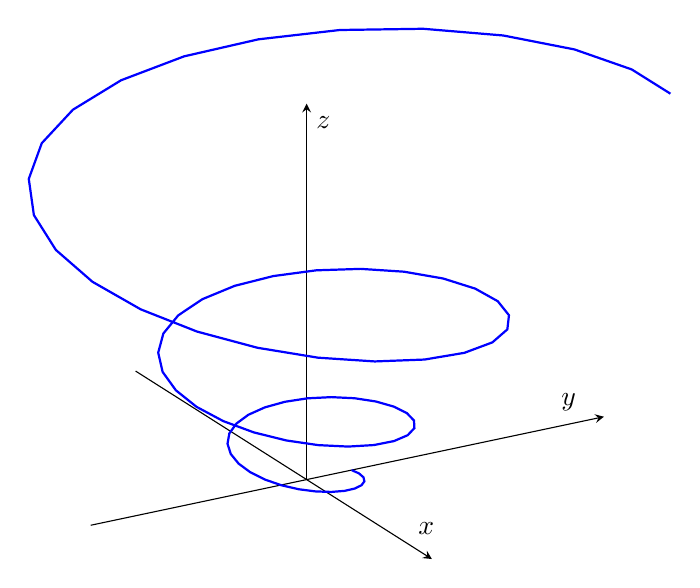
\begin{tikzpicture}
  \begin{axis}[
    view={60}{30},
    axis lines=center,
    xlabel={$x$}, ylabel={$y$}, zlabel={$z$},
    domain=0:2,
    samples=80,
    variable=t,
    xtick=\empty, ytick=\empty, ztick=\empty,
    restrict z to domain=0:7,
    scale=1.5,
  ]
    \addplot3[thick, blue] (
      {exp(t)*sin(deg(10*t))},
      {exp(t)*cos(deg(10*t))},
      {exp(t)}
    );
  \end{axis}
\end{tikzpicture}
\end{center}

\item The length of the parametrized curve $\mathbf{r}(t)=\left\langle x(t),\,y(t),\,z(t)\right\rangle$ for $a<t<b$ can be evaluated using the integral
\[L=\int_a^b\left|\frac{d\mathbf r}{dt}\right|\,dt\]

The length of the curve is then
\begin{align*}L&=\int_0^1\left|\frac{d\mathbf r}{dt}\right|\,dt=\int_0^1\left|\left\langle e ^t\sin t+ e ^t\cdot\cos t,\: e ^t\cos t- e ^t\sin t,\: e ^t\right\rangle\right|\,dt\\[1em]&=\int_0^1\sqrt{\left( e ^t\sin t+ e ^t\cdot\cos t\right)^2+\left( e ^t\cos t- e ^t\sin t\right)^2+\left( e ^t\right)^2}\,dt\\[1em]&=\int_0^1\sqrt{\scriptstyle e ^{2t}\left(\sin^2t+2\sin t\cos t+\cos^2t\right)+ e ^t\left(\cos^2t-2\sin t\cos t+\sin^2t\right)+ e ^{2t}}\,dt\\[1em]&=\int_0^1\sqrt{3 e ^{2t}}\,dt=\int_0^1\sqrt3 e^t\,dt=\sqrt3 e ^t\bigg|_0^1=\boxed{\sqrt3( e-1)}\end{align*}

\end{enumerate}

\item \begin{enumerate}[leftmargin=*,label=\textbf{\alph*.}]

\item Factor the denominator.
\begin{align*}\lim_{(x,y)\to(-1,-2)}\frac{y+2}{x^2y-xy+2x^2-2x}&=\lim_{(x,y)\to(-1,-2)}\frac{y+2}{x^2(y+2)-x(y+2)}\\[1em]&=\lim_{(x,y)\to(-1,-2)}\frac1{x^2-x}=\frac1{1-(-1)}=\boxed{\frac12}\end{align*}

\item Apply the Two-Path Test.
\[y=x\implies\lim_{(x,y)\to(0,0)}\frac{4x^2y}{x^4+y^2}=\lim_{(x,y)\to(0,0)}\frac{4x^3}{x^4+x^2}=\lim_{x\to0}\frac{4x}{x^2+1}=\frac01=0\]
\[y=x^2\implies\lim_{(x,y)\to(0,0)}\frac{4x^2y}{x^4+y^2}=\lim_{x\to0}\frac{4x^4}{2x^4}=\lim_{x\to0}\frac42=2\]

Since $0\neq2$, by the Two-Path Test, $\boxed{\text{the limit does not exist}}$.

\end{enumerate}

\item \begin{enumerate}[leftmargin=*,label=\textbf{\alph*.}]

\item Compute the first partial derivatives.
\[f_x=\frac1{x^2+y^2}\cdot2x=\frac{2x}{x^2+y^2},\qquad f_y=\frac1{x^2+y^2}\cdot2y=\frac{2y}{x^2+y^2}\]

Compute the second partial derivatives.
\[f_{xx}=\frac{2\left(x^2+y^2\right)-(2x)\cdot(2x)}{\left(x^2+y^2\right)^2}=\frac{2y^2-2x^2}{\left(x^2+y^2\right)^2}\]\[f_{yy}=\frac{2\left(x^2+y^2\right)-(2y)\cdot(2y)}{\left(x^2+y^2\right)^2}=\frac{2x^2-2y^2}{\left(x^2+y^2\right)^2}\]
\[f_{xx}+f_{yy}=\frac{2y^2-2x^2}{\left(x^2+y^2\right)^2}+\frac{2x^2-2y^2}{\left(x^2+y^2\right)^2}=\boxed0\]

\item\leavevmode

\vspace{-1em}
\begin{center}
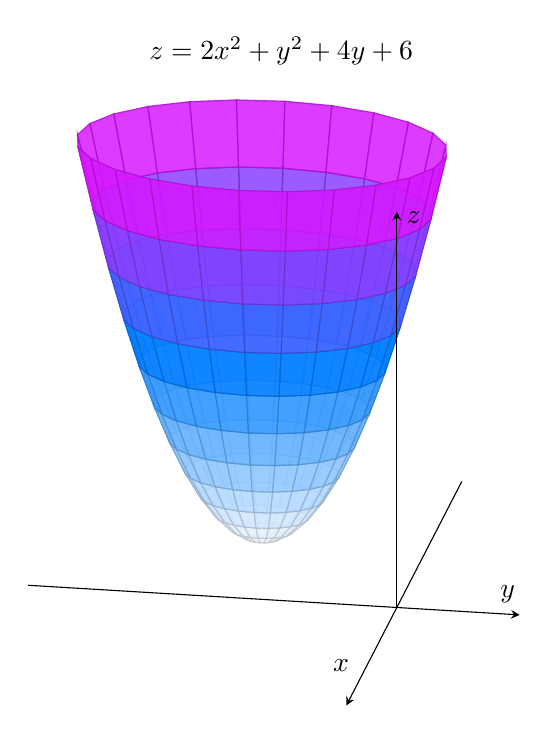
\begin{tikzpicture}
  \begin{axis}[
    title={$z=2x^2+y^2+4y+6$},
    title style={yshift=-10pt},
      view={100}{20},
      axis lines=center,
      axis equal image,
      xlabel={$x$},
      ylabel={$y$},
      zlabel={$z$},
      domain=0:2*pi,
      y domain=-2.25:2.25,
      samples=25,
      samples y=25,
      colormap/cool,
      axis on top,
      scale=1.5,
      xtick=\empty, ytick=\empty, ztick=\empty,
      z buffer=sort,
      xmin=-4.5, xmax=3.5,
      ymin=-4.5, ymax=1.5,
    ]
    \addplot3[
      surf,
      opacity=0.6
    ]
    ( {-2+(1/sqrt(2))*y*cos(deg(x))},
      {y*sin(deg(x))-2},
      {y^2} );
  \end{axis}
\end{tikzpicture}
\end{center}
\end{enumerate}
\end{enumerate}

\newpage
\stepcounter{subsection}
\phantomsection
\addcontentsline{toc}{subsection}{\protect\numberline{\thesubsection}Midterm - Spring 2016 Solutions}

\fancyhead[R]{\textit{2015-2016 Spring Midterm}}

%Last update: 28/8/26 (28th of August) 11:10

\begin{enumerate}[leftmargin=*,label=\textbf{\arabic*.}]
\item \begin{enumerate}[leftmargin=*,label=\textbf{\alph*.}]
\item The length of a parametrized curve can be calculated with the formula
\[L=\int_a^b\sqrt{\left(\frac{dy}{dt}\right)^2+\left(\frac{dx}{dt}\right)^2}\,dt.\]

Find the derivatives of $x$ and $y$ with respect to $t$.
\[\frac{dx}{dt}=-\sin t\cos t - (1+\cos t)\sin t, \quad \frac{dy}{dt}=-\sin^2 + (1+\cos t)\cos t\]

Then
\[\left(\frac{dx}{dt}\right)^2=\sin^2t\cos^2t+2\sin^2t\cos t(1+\cos t)+(1+\cos t)^2\sin^2t,\]
\[\left(\frac{dy}{dt}\right)^2=\sin^4t-2\sin^2t(1+\cos t)\cos t+(1+\cos t)^2\cos ^2 t.\]

The middle terms cancel each other in the addition. Recall the trigonometric identities $\sin^2t+\cos^2t=1$ and $\cos 2t=2\cos^2 t-1$. We have
\begin{align*}\left(\frac{dx}{dt}\right)^2+\left(\frac{dy}{dt}\right)^2&=\sin^2t\cos^2t+(1+\cos t)^2\sin^2t+\sin^4t+(1+\cos t)^2\cos^2t\\[1em]&=\sin^2t\cos^2t+\sin^4t+(1+\cos t)^2\sin^2t+(1+\cos t)^2\cos^2t\\[1em]&=\sin^2t(\sin^2t+\cos^2t)+(1+\cos t)^2(\cos^2t+\sin^2t)\\[1em]&=\sin^2t+(1+\cos t)^2\\[1em]&=\sin^2t+1+2\cos t+\cos^2t=2+2\cos t =4\cos^2\frac t2.\end{align*}

The length of the curve is
\[L=\int_{0}^{2\pi}\sqrt{4\cos^2\frac t2}\,dt=\int_0^{2\pi}2\left|\cos\frac t2\right|\,dt=2\cdot 2\int_0^{\pi}\cos\frac t2\,dt=\left.4\cdot\frac{\sin\frac t2}{\frac12}\right|_0^\pi=\boxed8.\]

\item Find the derivative of the parametric equation with respect to $t$.
\[\frac{d\vec r}{dt}=\frac d{dt}\left(t\right)\,\vec i+\frac d{dt}\left(t^2\right)\,\vec j+\frac d{dt}\left(t^3\right)\,\vec k=\vec i+ 2t\,\vec j+3t^2\,\vec k\]

Evaluate $\vec r$ and $\vec {r'}$ at $t=2$.
\[\left.\vec r\,\right|_{t=2}=\vec i+ 4\vec j+8\vec k,\quad \left.\vec{r'}\right|_{t=2}=2\vec i+4\vec j+8\vec k\]

The parametric equations for a line that passes through the point $P_0(x_0,y_0,z_0)$ is given by
\[\left.\begin{array}{c}
x=r_1+r_1't\\
y=r_2+r_2't\\
z=r_3+r_3't
\end{array}\right\}\quad t\in\mathbb{R}.\]

Therefore, the parametric equations for the line $L$ is
\[\boxed{\left.\begin{array}{l}
x=2+t\\
y=4+4t\\
z=8+12t
\end{array}\right\}\quad t\in\mathbb{R}}.\]

\end{enumerate}

\item \begin{enumerate}[leftmargin=*,label=\textbf{\alph*.}]
\item The gradient of each function is below.
\[\boxed{\begin{aligned}
\nabla f=\left\langle f_x, f_y\right\rangle&=\left\langle2xy, x^2\right\rangle\\
\nabla g=\left\langle g_x, g_y\right\rangle&=\left\langle3x^2, 10y\right\rangle
\end{aligned}}
\]

\item Since $\vec u$ is a unit vector, we have $|\vec u|=\sqrt{a^2+b^2}=1$. The directional derivatives along the unit vector $\vec u$ evaluated at $P_0$ are
\[D_{\vec u}f(P_0)=\nabla f\cdot\left.\vec u\right|_{P_0}=\left\langle4,4\right\rangle\cdot\left\langle a,b\right\rangle=4a+4b,\]
\[D_{\vec u}g(P_0)=\nabla g\cdot\left.\vec u\right|_{P_0}=\left\langle12,10\right\rangle\cdot\left\langle a,b\right\rangle=12a+10b.\]

We have $D_{\vec u}f(P_0)=D_{\vec u}g(P_0)$.
\[4a+4b=12a+10b\implies b=-\frac{4a}{3}\]

Along with $\sqrt{a^2+b^2}=1$, we find
\[\sqrt{a^2+b^2}=1\implies a^2+\left(\frac{-4a}3\right)^2=1\implies25a^2=9\implies a=\pm\frac{5}{3}.\]

Hence
\[\boxed{\vec u=\frac35\vec i-\frac45\vec j\quad \text{or}\quad\vec u=-\frac35\vec i+\frac45\vec j}.\]

\item Since $\vec v$ is not a unit vector, define the unit vector $\vec w=\dfrac{\vec v}{\left|\vec v\right|}=\dfrac{\vec i+\vec j}{\sqrt2}$.

Set the directional derivatives to $0$.
\[D_{\vec w}f=0\implies \nabla f\cdot \vec w=0\implies\left\langle2xy,x^2\right\rangle\cdot\left\langle\frac1{\sqrt2},\frac1{\sqrt2}\right\rangle=0\implies2xy+x^2=0\]
\[D_{\vec w}g=0\implies \nabla g\cdot \vec w=0\implies\left\langle3x^2,10y\right\rangle\cdot\left\langle\frac1{\sqrt2},\frac1{\sqrt2}\right\rangle=0\implies3x^2+10y=0\]

Factor $x$ in the first equation.
\[x(2y+x)=0\implies x=0\text{ or }x=-2y\]

Consider the second equation with the relations found above.
\[3x^2+10y=0\implies\left\{\begin{array}{l}x=0\implies y=0\\x=-2y\implies y(12y+10)=1\implies y=0\text{ or }y=-\frac{10}{12}\end{array}\right.\]

All the points are $\boxed{(x,y)=(0,0)\text{ and }(x,y)=\left(\frac53,-\frac{5}{6}\right)}$.

\end{enumerate}

\item \begin{enumerate}[leftmargin=*,label=\textbf{\alph*.}]
\item Along any line through the origin (except the vertical line) can be defined by $y=mx$. Along $y=mx$,
\begin{align*}\lim_{(x,y)\to(0,0)}f(x,y)&=\lim_{x\to0}f(x,mx)=\lim_{x\to0}\frac{x^3(m^4x^4)}{x^4+x^3(m^2x^2)+m^{10}x^{10}}\\[1em]&=\lim_{x\to0}\frac{m^4x^3}{1+m^2x+m^{10}x^6}=\frac01=\boxed0.\end{align*}

Check the vertical line. Along $x=0$,
\[f(0,y)=0\implies\lim_{(x,y)\to(0,0)}f(x,y)=\boxed0.\]

\item We earlier showed that the limit along any line through the origin is $0$. Apply the Two-Path test. Try $x=-y^2$.
\[\lim_{(x,y)\to(0,0)}f(x,y)=\lim_{y\to0}f\left(-y^2,y\right)=\lim_{y\to0}\frac{-y^6y^4}{y^8-y^6y^2-y^{10}}=\lim_{y\to0}\frac{-y^{10}}{y^{10}}=-1\neq0\]

Since we have two different limits, the limit $\displaystyle\lim_{(x,y)\to(0,0)}f(x,y)$ does not exist.

\end{enumerate}

\item Obtain the partial derivatives and set to $0$.
\[f_x=4x+4xy=0\implies 4x(1+y)=0\implies x=0 \text{ or } y=-1\]
\[f_y=2y+2x^2=0\implies\left\{\begin{array}{l}x=0\implies y=0\\ y=-1\implies x=\pm 1\end{array}\right.\]

Thus the critical points are $(0,0),~(1,-1)$ and $(-1,-1)$. Obtain the Hessian determinant.
\[f_{xx}=4+4y,\quad f_{yy}=2,\quad f_{xy}=f_{yx}=4x\]
\[D=\begin{vmatrix}f_{xx} & f_{xy} \\f_{yx} & f_{yy}\end{vmatrix}=f_{xx}f_{yy}-f_{xy}^2=8+8y-16x^2\]

Evaluate $D$ at the points.
\[D(0,0)=8>0,\quad f_{yy}(0,0)=2>0\implies (0,0)\text{ is a local minimum.}\]
\[D(1,-1)=-16<0\implies (0,0)\text{ is a saddle point.}\]
\[D(-1,-1)=-16<0\implies (0,0)\text{ is a saddle point.}\]
\[\boxed{(0,0)\text{ is a local minimum. }(1,-1)\text{ and }(-1,-1)\text{ are saddle points.}}\]
\item The extreme value theorem states that a continuous function on a specific region will always reach its absolute highest and lowest values.

On the interior of $D$,
\[f_x=4(x^2+y^2-1)2x+2x=2x\left[4\left(x^2+y^2\right)-3\right]=0,\]
\[f_y=4(x^2+y^2-1)2y-2y= 2y\left[4\left(x^2+y^2\right)-5\right]=0.\]

From the first equality, we have $x=0$ or $x^2+y^2=\frac34$.

From the second one, if $x=0$, then $y=0$ or $y=\pm\frac{\sqrt5}2\notin D$.

If $x^2+y^2=\frac34$, then $y=0$. Therefore, $x=\pm\frac{\sqrt3}2$.

So the critical points are $(0,0)$, $\left(\frac{\sqrt3}2,0\right)$ and $\left(-\frac{\sqrt3}2,0\right)$.

On the boundary of $D$,
\[x^2+y^2=1\implies y^2=1-x^2\implies y=\pm\sqrt{1-x^2},\]
\[f\left(x,\pm \sqrt{1-x^2}\right)=2(x^2+1-x^2-1)^2+x^2-1+x^2=2x^2-1.\]

Find the critical points on the boundary.
\[f'\left(x,\pm\sqrt{1-x^2}\right)=4x=0\]

At $x=0$, $y\pm1$. The critical points are $(0,1)$ and $(0,-1)$.

The end points are $(1,0)$ and $(-1,0)$.

Evaluate $f$ at all the aforementioned points and compare the values.
\[f(0,0)=2,\qquad f(0,1)=f(0,-1)=-1\]
\[f(1,0)=f(-1,0)=1,\qquad f\left(\sqrt3/2, 0\right)=f\left(-\sqrt3/2,0\right)=7/8\]

\end{enumerate}

\newpage
\stepcounter{subsection}
\phantomsection
\addcontentsline{toc}{subsection}{\protect\numberline{\thesubsection}Midterm - Spring 2020 Solutions}

\fancyhead[R]{\textit{2019-2020 Spring Midterm}}

%(Last update: 19/8/25 (19th of August) 18:27)

\begin{enumerate}[leftmargin=*,label=\textbf{\arabic*.}]

\item Let $M$ be the line
\[\dfrac{x-2}{-1}=\dfrac{y-1}{-2}=\dfrac{z-5}{1}=\lambda,\quad\lambda\in\mathbb{R}.\]

The direction vector of $M$ is $\mathbf u=\left\langle-1,-2,1\right\rangle$.

Let $\mathbf v=\left\langle a,b,c\right\rangle$, where $a,b,c\in\mathbb R$, be the direction vector of $L$. If $M$ and $L$ are orthogonal, the dot product of the direction vectors is zero.
\[\mathbf u\cdot\mathbf v=\left\langle1,-2,1\right\rangle\cdot\left\langle a,b,c\right\rangle=a-2b+c=0\]

$a,b,c$ could be any number with the relation $a-2b+c=0$. Let $a=1,\, b=1$. Then $c=2b-a=2-1=1$. The direction vector $\mathbf v$ is then $\mathbf v=\left\langle1,1,3\right\rangle$.

The parametric equations for a line that passes through the point $P_0(x_0,y_0,z_0)$ is given by
\[\left.\begin{array}{c}
x=x_0+v_1t\\
y=y_0+v_2t\\
z=z_0+v_3t
\end{array}\right\}\quad t\in\mathbb{R}\]

Therefore, using the point $P$, the parametric equations for the line $L$ is

\[\boxed{\left.\begin{array}{l}
x=-1+t\\
y=3+t\\
z=1+3t
\end{array}\right\}\quad t\in\mathbb{R}}\]

\item \begin{enumerate}[leftmargin=*,label=\textbf{\alph*.}]
\item Exponential surface
\begin{center}
    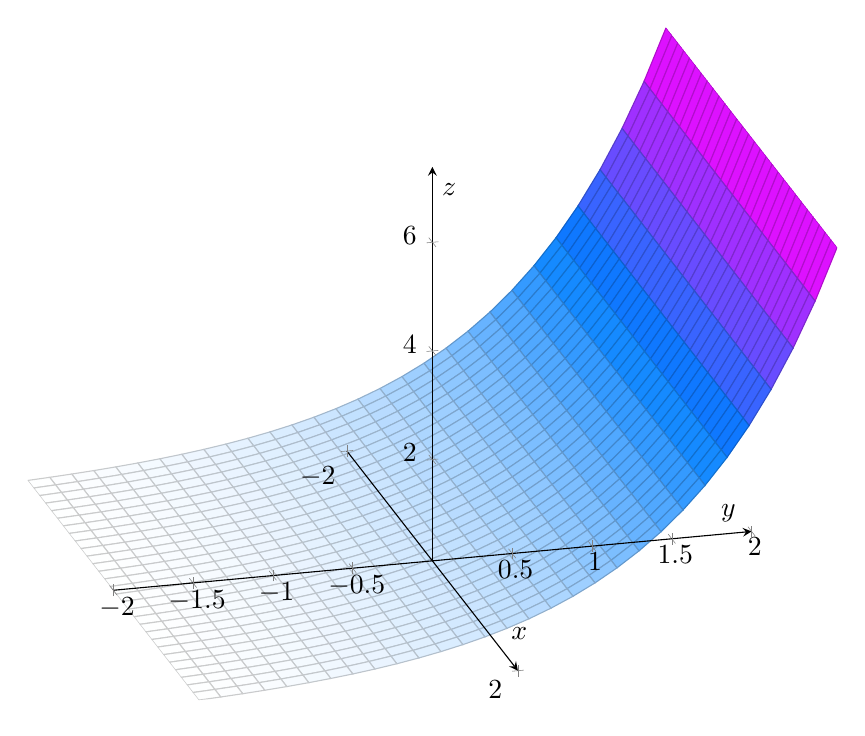
\begin{tikzpicture}
  \begin{axis}[
    view={75}{30},
    axis lines=center,
    xlabel={$x$},
    ylabel={$y$},
    zlabel={$z$},
    domain=-2:2,
    samples=30,
    colormap/cool,
    mesh/ordering=y varies,
    scale=1.5,
    axis on top,
  ]
    \addplot3[surf]  (x, y, {e^y});
  \end{axis}
\end{tikzpicture}
\end{center}

\newpage
\item Hyperbolic paraboloid
\begin{center}
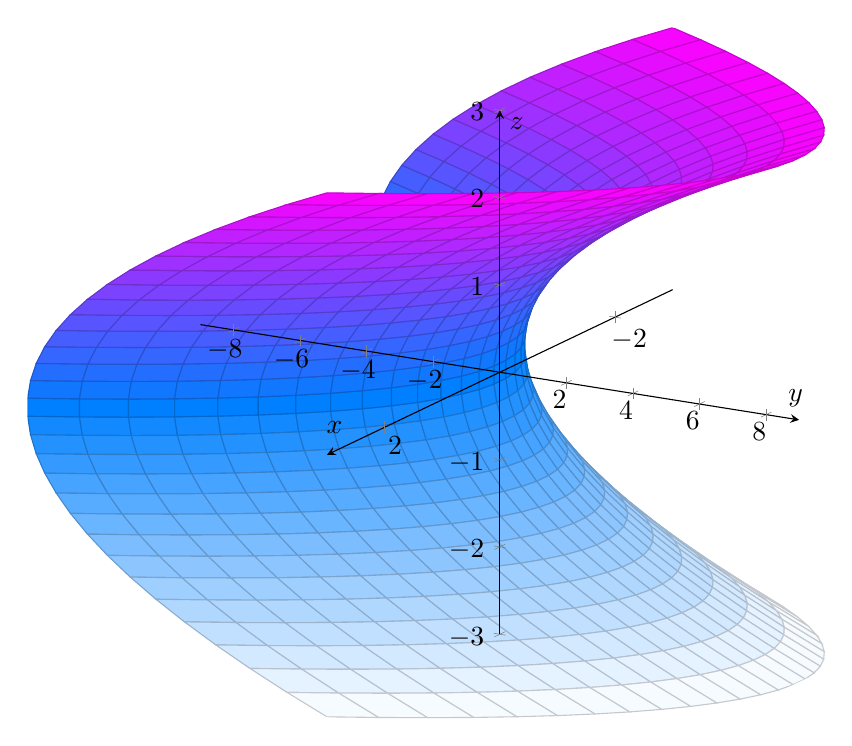
\begin{tikzpicture}
  \begin{axis}[
    view={120}{20},
    axis lines=center,
    xlabel={$x$},
    ylabel={$y$},
    zlabel={$z$},
    domain=-3:3,
    y domain=-3:3,
    samples=30,
    samples y=30,
    colormap/cool,
    z buffer=sort,
    axis on top,
    scale=1.75
  ]
    \addplot3[surf]({x}, {y^2 - x^2}, {y});
  \end{axis}
\end{tikzpicture}
\end{center}

\end{enumerate}

\item The velocity and acceleration vectors can be obtained by taking the first and the second derivatives of the vector function with respect to the parametrization variable, respectively.

\[\text{Velocity vector}:\mathbf v(t)=\frac{d\mathbf R}{dt}=\left\langle-2\sin t,\,2t,\,2\cos t\right\rangle\]
\[\text{Acceleration vector}:\mathbf a(t)=\frac{d\mathbf v}{dt}=\left\langle-2\cos t,\,2,\,-2\sin t\right\rangle\]

The speed of motion is the magnitude of the velocity vector, and the direction is the normalized velocity vector.

\[\text{Speed}=\left|\mathbf v(t=\pi/2)\right|=\sqrt{\left(-2\sin\frac\pi2\right)^2+\left(2\cdot\frac\pi2\right)^2+\left(2\cos\frac\pi2\right)^2}=\sqrt{4+\pi^2}\]
\[\text{Direction}=\frac{\mathbf v(t=\pi/2)}{\left|\mathbf v(t=\pi/2)\right|}=\frac{\left\langle-2\sin\dfrac\pi2,\,2\cdot\dfrac\pi2,\,2\cos\dfrac\pi2\right\rangle}{\sqrt{4+\pi^2}}=\left\langle-\frac2{\sqrt{4+\pi^2}},\,\frac\pi{\sqrt{4+\pi^2}},0\right\rangle\]

\[\boxed{\begin{array}{c}
\mathbf v(t)=\left\langle-2\sin t,\,2t,\,2\cos t\right\rangle\\
\mathbf a(t)=\left\langle-2\cos t,\,2,\,-2\sin t\right\rangle\\[1em]
\text{Speed of motion at }t=\dfrac\pi2:\sqrt{4+\pi^2}\\
\text{Direction of motion at }t=\dfrac\pi2:\left\langle-\dfrac2{\sqrt{4+\pi^2}},\,\dfrac\pi{\sqrt{4+\pi^2}},0\right\rangle\\
\end{array}}\]

\newpage

\item Apply the Two-Path Test.
\[x=y\implies\lim_{(x,y)\to(0,0)}\frac{xy^3}{x^2+y^6}=\lim_{y\to0}\frac{y^4}{y^2+y^6}=\lim_{y\to0}\frac{y^2}{1+y^4}=\frac01=0\]
\[x=y^3\implies\lim_{(x,y)\to(0,0)}\frac{xy^3}{x^2+y^6}=\lim_{y\to0}\frac{y^6}{y^6+y^6}=\lim_{y\to0}\frac{y^6}{2y^6}=\frac12\]

Since $0\neq\dfrac12$, by the Two-Path Test, the limit does not exist. Therefore, the function $f$ is not continuous at $(0,0)$.

\item The value of the function at the point $(0,0)$ is $0$. Therefore, we will show that the limit $L$ is also $0$. For every $\epsilon>0$, there exists a $\delta>0$ such that
\[0<\sqrt{(x-0)^2+(y-0)^2}<\delta\implies\left|f(x,y)-L\right|<\epsilon.\]
\begin{align*}\left|\frac{x^2y}{x^2+y^6}-0\right|&=|y|\cdot\left|\frac{x^2}{x^2+y^6}\right|\leq|y|\cdot1=|y|\qquad\left[\frac{x^2}{x^2+y^6}\leq\frac{x^2}{x^2}=1\right]\\[1em]&\leq|x|+|y|<2\delta\quad\left[x^2\geq0,\,y^2\geq0,\,\sqrt{x^2+y^2}<\delta\implies|x|<\delta,\,|y|<\delta\right]\end{align*}

Let $\delta=\dfrac\epsilon2$. Then
\[\left|\frac{x^2y}{x^2+y^6}\right|\leq|x|+|y|=2\cdot\frac\epsilon2=\epsilon.\]

Since the limit is equal to the value of the function at $(0,0)$, $f$ is continuous at $(0,0)$.

\item $u$ and $v$ are functions of $x$ and $y$. $x$ and $y$ are functions of $r$ and $\theta$. Use the chain rule.

\[\frac{\partial u}{\partial r}=\frac{\partial u}{\partial x}\cdot\frac{\partial x}{\partial r}+\frac{\partial u}{\partial y}\cdot\frac{\partial y}{\partial r}=u_x\cdot\cos\theta+u_y\cdot\sin\theta=v_y\cos\theta-v_x\sin\theta\]

\[\frac{\partial v}{\partial\theta}=\frac{\partial v}{\partial x}\cdot\frac{\partial x}{\partial\theta}+\frac{\partial v}{\partial y}\cdot\frac{\partial y}{\partial\theta}\implies\frac1r\frac{\partial v}{\partial\theta}=\frac1r\left(-v_x\cdot r\sin\theta+v_y\cdot r\cos\theta\right)=-v_x\sin\theta+v_y\cos\theta\]

\[\frac{\partial u}{\partial r}=-v_x\sin\theta+v_y\cos\theta=\frac1r\frac{\partial v}{\partial\theta}\]

\[\frac{\partial v}{\partial r}=\frac{\partial v}{\partial x}\cdot\frac{\partial x}{\partial r}+\frac{\partial v}{\partial y}\cdot\frac{\partial y}{\partial r}=v_x\cdot\cos\theta+v_y\cdot\sin\theta=-u_y\cos\theta+u_x\sin\theta\]

\[\frac{\partial u}{\partial\theta}=\frac{\partial u}{\partial x}\cdot\frac{\partial x}{\partial\theta}+\frac{\partial u}{\partial y}\cdot\frac{\partial y}{\partial\theta}\implies-\frac1r\frac{\partial u}{\partial\theta}=-\frac1r\left(-u_x r\sin\theta+u_y r\cos\theta\right)=u_x\sin\theta-u_y\cos\theta\]

\[\frac{\partial v}{\partial r}=u_x\sin\theta-u_y\cos\theta=-\frac1r\frac{\partial u}{\partial \theta}\]

Therefore, the Cauchy-Riemann equations hold.

\item The total differential of $R$ is
\[dR=\frac{\partial R}{\partial x}\,dx+\frac{\partial R}{\partial r}\,dr=\frac c{r^4}\,dx-\frac{4cx}{r^5}\,dr\]

Since we estimate the percent change in $R$, we may take $\Delta R\approx dR$. Therefore, $dx=x\cdot3\%,\,dr=r\cdot(-2\%)$. Given also $x=8\,\text{cm},\,r=2\, \text{mm}=0.2\,\text{cm}$, the percent change can be estimated as
\[\frac{dR}R\cdot100\%=\frac1{\frac{cx}{r^4}}\cdot\left(\frac c{r^4}\cdot x\cdot3\%-\frac{4cx}{r^5}\cdot r\cdot(-2\%)\right)\cdot100\%=\boxed{11\%}\]

\item To identify the critical points, find where both $f_x=f_y=0$ or one of the partial derivatives does not exist.
\[f_x=-3x^2+9,\quad f_y=-8y\]
\[\left.\begin{array}{c}
f_x=0\implies9=3x^2\\
f_y=0\implies-8y=0 
\end{array}\:\right\}\quad y=0,\:x=\pm\sqrt3\]

The critical points are $\left(\sqrt3,0\right)$ and $\left(-\sqrt3,0\right)$. To classify these points, calculate the second partial derivatives and then find the Hessian determinants.
\[f_{xx}=-6x,\quad f_{xy}=f_{yx}=0,\quad f_{yy}=-8\]
\[\left(\sqrt3,0\right)\rightarrow\left\{\:\begin{array}{l}
f_{xx}=-6\sqrt3,\quad f_{xy}=0,\quad f_{yy}=-8\\[1em]
\left|\begin{array}{cc}
-6\sqrt3 & 0\\
0 & -8
\end{array}\right|=\left(-6\sqrt3\right)\cdot(-8)-0\cdot0=48\sqrt3>0,\quad f_{xx}<0
\end{array}\right.\]

\[\left(-\sqrt3,0\right)\rightarrow\left\{\:\begin{array}{l}
f_{xx}=6\sqrt3,\quad f_{xy}=0,\quad f_{yy}=-8\\[1em]
\left|\begin{array}{cc}
6\sqrt3 & 0\\
0 & -8
\end{array}\right|=\left(-6\sqrt3\right)\cdot(-8)-0\cdot0=-48\sqrt3<0
\end{array}\right.\]

\[\boxed{\text{A local maximum occurs at }\left(\sqrt3,0\right)\text{ and a saddle point occurs at }\left(-\sqrt3,0\right).}\]
\end{enumerate}

\newpage
\stepcounter{subsection}
\phantomsection
\addcontentsline{toc}{subsection}{\protect\numberline{\thesubsection}Midterm - Summer 2020 Solutions}

\fancyhead[R]{\textit{2019-2020 Summer Midterm}}

%Last update: 30/08/2025 01:52

\begin{enumerate}[leftmargin=*,label=\textbf{\arabic*.}]
\item The normal vector of the plane is the gradient vector. Find the normal vectors of the planes and calculate the cross product of these vectors. The resulting vector is parallel to the intersection of the planes.
\[\mathbf{n}_1=\left\langle1,-1,0\right\rangle,\qquad \mathbf{n}_2=\left\langle3,0,1\right\rangle\]
\[\mathbf{v}=\mathbf{n}_1\times\mathbf{n}_2=\left|\begin{array}{ccc}
\mathbf{i}&\mathbf{j}&\mathbf{k}\\
1&-1&0\\
3&0&1
\end{array}\right|=\mathbf{i}\left|\begin{array}{cc}
-1&0\\0&1
\end{array}\right|-\mathbf{j}\left|\begin{array}{cc}
1&0\\3&1
\end{array}\right|+\mathbf{k}\left|\begin{array}{cc}
1&-1\\3&0
\end{array}\right|=-\mathbf{i}-\mathbf{j}+3\mathbf{k}\]

The parametric equations for a line passing through the point $P_0(x_0,y_0,z_0)$ is given by
\[\left.\begin{array}{c}
x=x_0+v_1t\\
y=y_0+v_2t\\
z=z_0+v_3t
\end{array}\right\}\quad t\in\mathbb{R}\]

Therefore, the parametric equations for the line $L$ is
\[\boxed{\left.\begin{array}{l}
x=-t\\
y=2-t\\
z=1+3t
\end{array}\right\}\quad t\in\mathbb{R}}\]

\item The vector that is parallel to the direction of the line is
\[\mathbf u=\left\langle-1-1,0-2,4-1\right\rangle=\left\langle-2,-2,3\right\rangle\]

If the vectors $\mathbf v$ and $\mathbf u$ are orthogonal, the dot product of these two vectors must be equal to zero.
\[\mathbf v\times \mathbf u=\left\langle1,5,4\right\rangle\cdot\left\langle-2,-2,3\right\rangle=1\cdot(-2)+5\cdot(-2)+4\cdot3=-2-10+12=\boxed{0}\]

\newpage
\item \begin{enumerate}[leftmargin=*,label=\textbf{\alph*.}]
\item Exponential surface
\begin{center}
    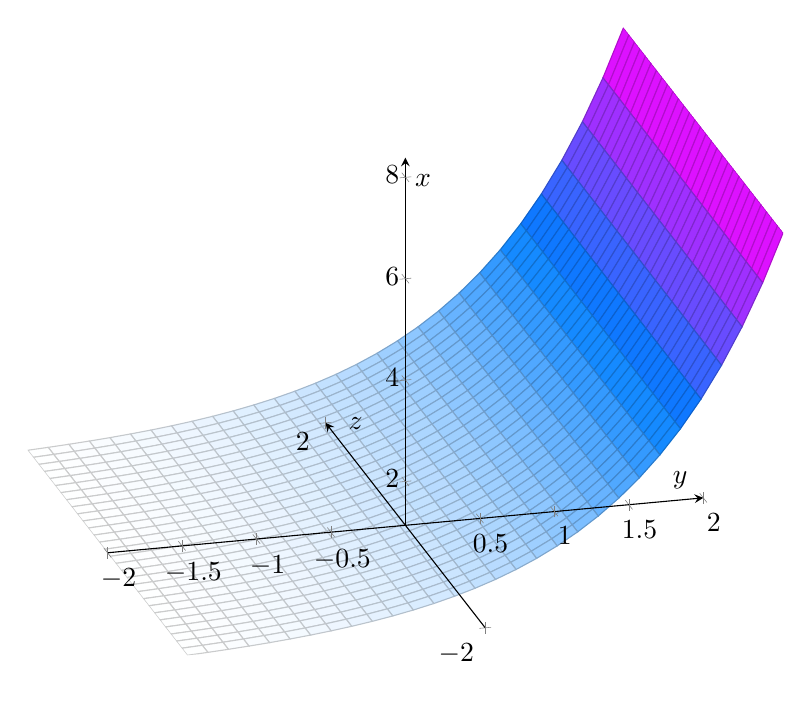
\begin{tikzpicture}
  \begin{axis}[
    view={-15}{30},
    axis lines=center,
    xlabel={$y$},
    ylabel={$z$},
    zlabel={$x$},
    domain=-2:2,
    samples=30,
    colormap/cool,
    mesh/ordering=y varies,
    scale=1.4,
    axis on top,
  ]
    \addplot3[surf]{exp(x)+1};
  \end{axis}
\end{tikzpicture}
\end{center}

\item Hyperboloid of one sheet
\begin{center}
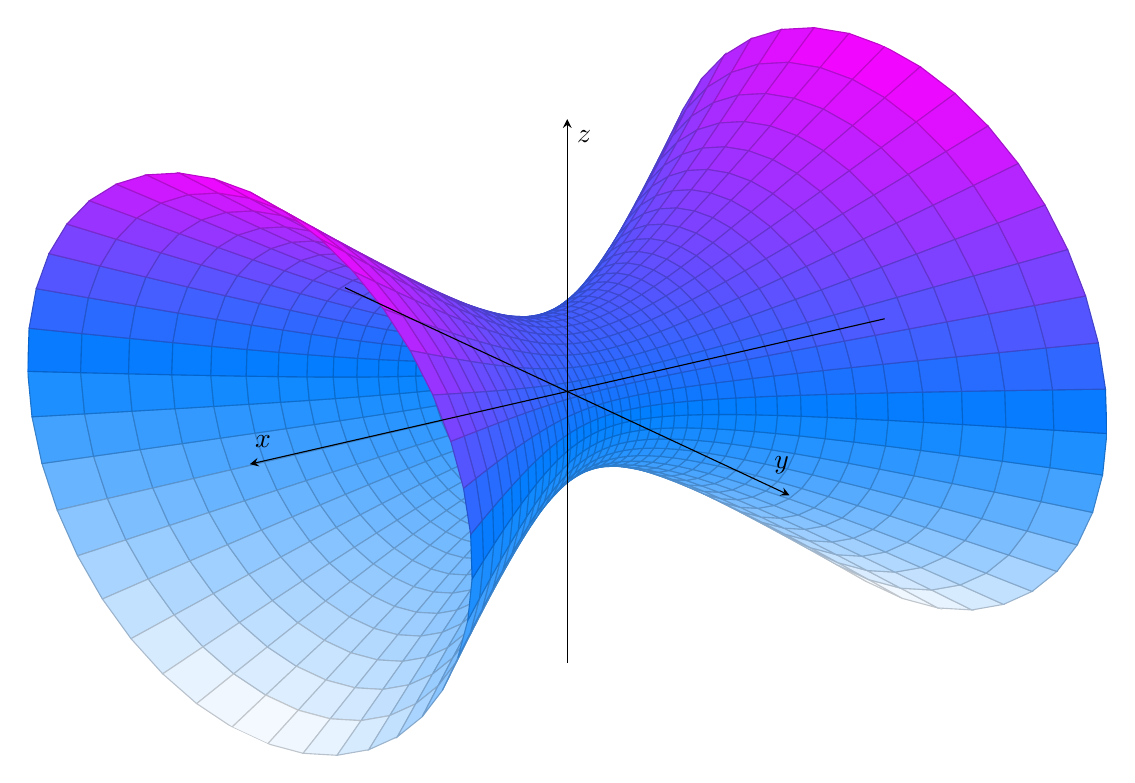
\begin{tikzpicture}
  \begin{axis}[
    view={145}{25},
    xlabel={$x$},
    ylabel={$y$},
    zlabel={$z$},
    axis lines=center,
    domain=0:360,
    y domain=-2:2,
    samples=40,
    axis on top,
    colormap/cool,
    scale=2,
    ticklabel style={anchor=base},
    z buffer=sort, 
    xtick=\empty, ytick=\empty, ztick=\empty,
  ]
  
  \addplot3[surf] ({sinh(y)},{cosh(y)*sin(x)},{cosh(y)*cos(x)});
  \end{axis}
\end{tikzpicture}
\end{center}
\end{enumerate}

\item Apply the Two Different Paths Test.

\[y=x\implies\lim_{(x,y)\to(0,0)}\frac{x^5y^3}{x^7+y^{21/2}}=\lim_{x\to0}\frac{x^8}{x^7\left(1+x^{7/2}\right)}=\lim_{x\to0}\frac x{1+x^{7/2}}=\frac01=0\]
\[y=x^{2/3}\implies\lim_{(x,y)\to(0,0)}\frac{x^5y^3}{x^7+y^{21/2}}=\lim_{x\to0}\frac{x^7}{2x^7}=\frac12\]

Since $0\neq\dfrac12$, by the Two Different Paths Test, the limit does not exist.

\newpage

\item For every $\epsilon>0$, there exists a $\delta>0$ such that

\[0<\sqrt{(x-0)^2+(y-0)^2}<\delta\implies\left|f(x,y)-L\right|<\epsilon\]

The value of the function at $(0,0)$ is $f(0,0)=6\cdot0^2+7\cdot0^2=0$. So, we expect that the limit of the function at this point is $0$.

\[\left|6x^2+7y^2\right|=6x^2+7y^2\qquad\left[x^2\geq0,\quad y^2\geq0\right]\]
\[6x^2+7y^2\leq7x^2+7y^2=7\left(x^2+y^2\right)<7\delta^2\qquad\left[0<\sqrt{x^2+y^2}<\delta\right]\]

Set $\delta=\sqrt{\dfrac\epsilon7}$.

\[\left|f(x,y)-L\right|=|6x^2+7y^2-0|=6x^2+7y^2<7\delta^2=\epsilon\]

Since the limit is the value of the function at this point, $\boxed{f \text{ is continuous}}$ at $(x,y)=(0,0)$.

\item $w$ is a function of $x,\:y,\:z$ and $x,\:y,\:z$ are functions of $r,\:s,\:t$. Namely, $w=w(x,y,z),\:x=x(r,s,t),\:y=y(r,s,t),\:z=z(r,s,t)$. Apply the chain rule.

\[\frac{\partial w}{\partial r}=\frac{\partial w}{\partial x}\cdot\frac{\partial x}{\partial r}+\frac{\partial w}{\partial y}\cdot\frac{\partial y}{\partial r}+\frac{\partial w}{\partial z}\cdot\frac{\partial z}{\partial r}\]

\[\frac{\partial w}{\partial x}={e}^{2x-y+3z^2}\cdot2,\quad\frac{\partial w}{\partial y}={e}^{2x-y+3z^2}\cdot(-1),\quad\frac{\partial w}{\partial z}={e}^{2x-y+3z^2}\cdot(6z)\]

\[\frac{\partial x}{\partial r}=1,\quad\frac{\partial y}{\partial r}=2,\quad\frac{\partial z}{\partial r}=-2\sin(rst)\cdot st\]

\[\frac{\partial w}{\partial r}=2{e}^{2x-y+3z^2}-2{e}^{2x-y+3z^2}-12z{e}^{2x-y+3z^2}\sin(rst)st=\boxed{-12zst\cdot{e}^{2x-y+3z^2}\cdot\sin(rst)}\]

\item The volume and the surface area of a right circular cylinder are as follows, respectively.
\[V(D,h)=\frac{\pi D^2h}4,\quad S(D,h)=\pi Dh+\frac{\pi D^2}2\]

$D$ is the diameter of the base and $D=2r$.

\begin{enumerate}[leftmargin=*,label=\textbf{\alph*.}]
\item The total differential of $V$ is

\[dV=V_D\cdot dD+V_h\cdot dh\]

Calculate the partial derivatives.

\[V_D=\frac{\pi Dh}2,\quad V_h=\frac{\pi D^2}4\]

It is given $\left|dD\right|\leq0.5,\:|dh|\leq0.5,\:D=4,\:h=8$. The bounds for the propagated error in calculating the volume is

\[|dV|\leq\frac{\pi\cdot4\cdot8}2\cdot0.5+\frac{\pi\cdot4^2}4\cdot0.5=8\pi+2\pi=\boxed{10\pi\:\text{cm}^3}\]

\item The total differential of $S$ is

\[dS=S_D\cdot dD+S_h\cdot dh\]

Calculate the partial derivatives.

\[S_D=\pi h+\pi D,\quad S_h=\pi D\]

It is given $\left|dD\right|\leq0.5,\:|dh|\leq0.5,\:D=4,\:h=8$. The bounds for the propagated error in calculating the surface area is

\[|dS|=\pi\left(8+4\right)\cdot0.5+4\pi\cdot0.5=6\pi+2\pi=\boxed{8\pi\:\text{cm}^2}\]
\end{enumerate}

\item The normal vector to the surface is $\left\langle0,\ln z,\frac yz+1\right\rangle$. At the point $(1,0,2)$, the normal vector is $\left\langle0,\ln2,1\right\rangle$. The dot product of the normal vector to the surface and the vector that is parallel to the direction of the line is $0$. Let $\mathbf v=\langle 0,b,c\rangle$ be the direction vector of the line. The $x$-component is $0$ because the line is parallel to the $yz$-plane.

\[\langle0,\ln2,1\rangle\cdot\langle0,b,c\rangle=b\ln2+c=\implies \frac cb=-\ln2\]

The slope of the line is $\dfrac{dz}{dy}$ on the $yz$-plane, which is $\dfrac cb$. Therefore, the slope is $\boxed{-\ln2}$.

\item The equation for the tangent plane to the surface defined by $z=f(x,y)$ at a point $P_0(x_0,y_0,z_0)$ is given by $z-z_0=f_x(x-x_0)+f_y(y-y_0)$.

\[x_0=0,\quad y_0=1,\quad z_0=3,\quad f_x=\cos x+y{e}^{xy},\quad f_y=x{e}^{xy}+2\]
\[P=(0,1,3)\quad\rightarrow\quad f_x(0,1)=2,\quad f_y(0,1)=2\]

The equation for the tangent plane is

\[\boxed{z-3=2(x-0)+2(y-1)\implies z=2x+2y+1}\]

\end{enumerate}

\newpage
\stepcounter{subsection}
\phantomsection
\addcontentsline{toc}{subsection}{\protect\numberline{\thesubsection}Midterm - Spring 2021 Solutions}

\fancyhead[R]{\textit{2020-2021 Spring Midterm}}

%Last update: 28/08/2025 14:04

\begin{enumerate}[leftmargin=*,label=\textbf{\arabic*.}]
\item
\begin{enumerate}[leftmargin=*,label=\textbf{\alph*.}]
\item \label{item:19_20_spring_midterm_1} Two lines are skew if they do not intersect and are not parallel.

Let $L$ be the line $x-1=\dfrac z3,\: y=0$  and $M$ be the line $\displaystyle x=\frac{y+1}2=z$. Let $\mathbf u$ and $\mathbf v$ be the vectors that are parallel to these lines, respectively. Using the coefficients from the symmetric equations, we have $\mathbf u=\langle1,0,3\rangle, \:\mathbf v= \langle1,2,1\rangle$. If the cross product of these vectors is a non-zero vector, they are not parallel.
\[\mathbf{n}=\mathbf{u}\times\mathbf{v}=\left|\begin{array}{ccc}
\mathbf{i}&\mathbf{j}&\mathbf{k}\\
1&0&3\\
1&2&1
\end{array}\right|=\mathbf{i}\left|\begin{array}{cc}
0&3\\2&1
\end{array}\right|-\mathbf{j}\left|\begin{array}{cc}
1&3\\1&1
\end{array}\right|+\mathbf{k}\left|\begin{array}{cc}
1&0\\1&2
\end{array}\right|=-6\mathbf{i}+2\mathbf{j}+2\mathbf{k}\neq\mathbf{0}\]

Parametrize the lines and determine whether they intersect.
\[L=\left\{\begin{array}{l}
x=1+t\\
y=0\\
z=3t
\end{array}\right.\quad t\in\mathbb{R}\qquad\qquad M=\left\{\begin{array}{l}
x=s\\
y=2s-1\\
z=s
\end{array}\right.\quad s\in\mathbb{R}\]

Compare the $y$-components. If $2s-1=0$, then $s=\dfrac12$. If we substitute the value for $s$ in the $x$- and $z$- components and compare, we obtain $1+t=\dfrac12$ and $3t=\dfrac12$.
\[1+t=\frac12\implies t=\frac12,\qquad 3t=\frac12\implies t=\frac32\]
\[\frac12\neq\frac32\]

This leads to a contradiction that the lines intersect. Since the lines do not intersect and are not parallel, the lines are skew.

\item From \ref{item:19_20_spring_midterm_1}, we have the normal vector $\mathbf n$ of the plane. The equation for the tangent plane with the normal vector $\mathbf n$ containing the point $P_0(x_0,y_0,z_0)$ is given by $n_1(x-x_0)+n_2(y-y_0)+n_3(z-z_0)=0$.

\[x_0=1,\quad y_0=3,\quad z=5,\quad \mathbf n=-6\mathbf{i}+2\mathbf{j}+2\mathbf{k}\]
The equation for the tangent plane is

\[-6(x-1)+2(y-3)+2(z-5)=0\implies\boxed{-3x+y+z=5}\]
\end{enumerate}
\newpage

\item \begin{enumerate}[leftmargin=*,label=\textbf{\alph*.}]
\item Conical surface \begin{center}
    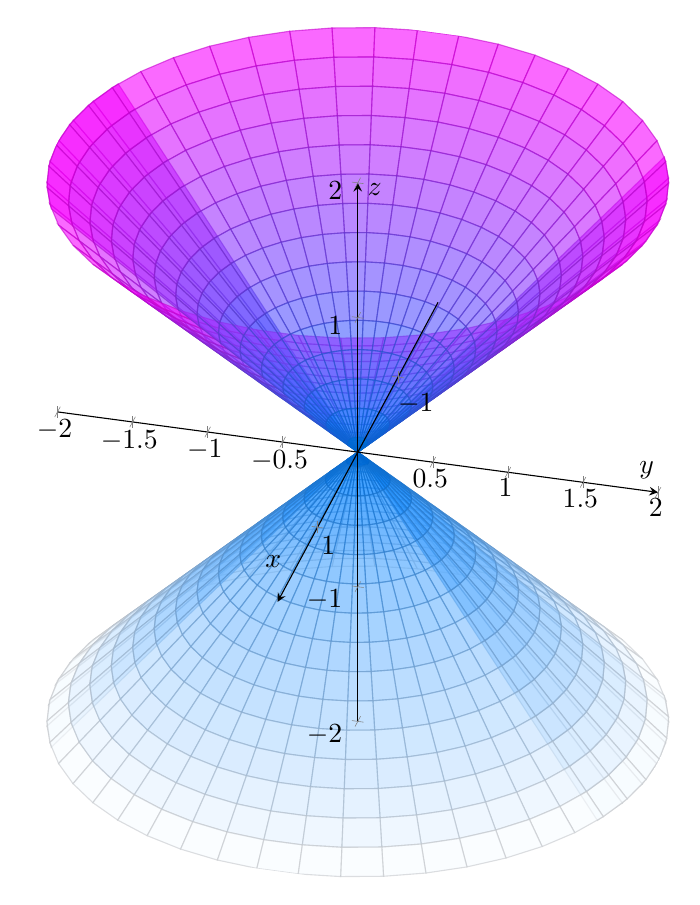
\begin{tikzpicture}
  \begin{axis}[
    view={105}{30},
    axis lines=center,
    axis equal image,
    xlabel={$x$},
    ylabel={$y$},
    zlabel={$z$},
    domain=-2:2,
    samples=30,
    colormap/cool,
    mesh/ordering=y varies,
    scale=3,
    axis on top,
  ]
  \addplot3 [surf,z buffer=sort,opacity=0.6] ({x*cos(deg(y))}, {x*sin(deg(y))}, {x});
  \addplot3 [surf,z buffer=sort,opacity=0.6] ({x*cos(deg(y))}, {x*sin(deg(y))}, {-x});
  \end{axis}
\end{tikzpicture}
\end{center}

\item Cylindrical surface \begin{center}
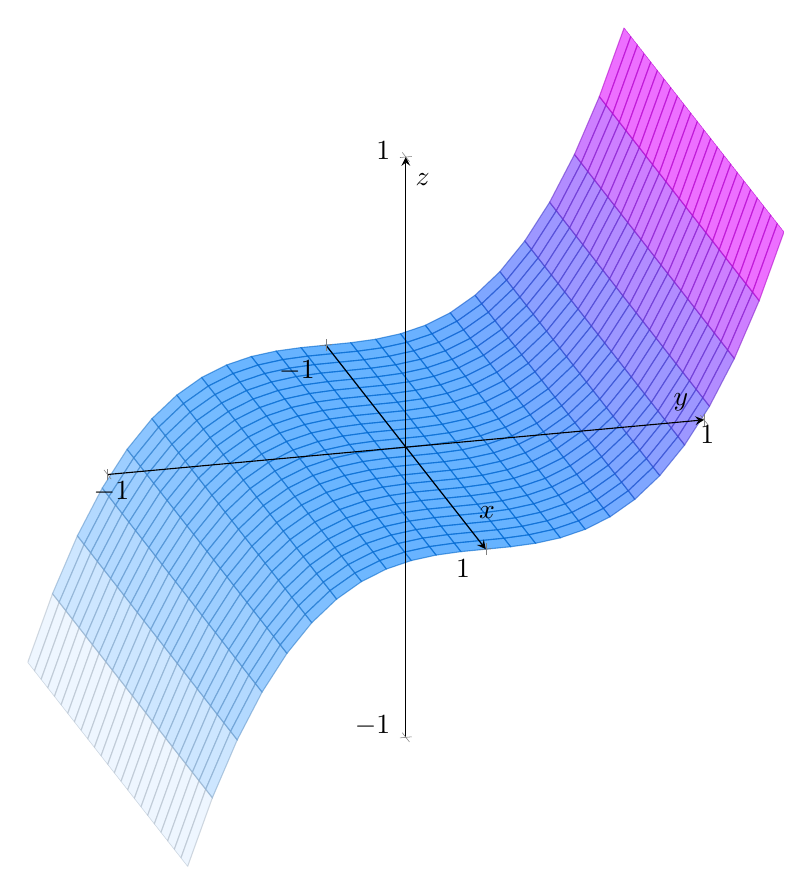
\begin{tikzpicture}
  \begin{axis}[
    view={75}{20},
    axis equal image,
    axis lines=center,
    xlabel={$x$},
    ylabel={$y$},
    zlabel={$z$},
    domain=-1:1,
    samples=25,
    colormap/cool,
    scale=2.2,
    axis on top,
    xtick={-1,1}, ytick={-1,1}, ztick={-1,1},
  ]
  \addplot3 [surf,z buffer=sort,opacity=0.6] {y^3};
  \end{axis}
\end{tikzpicture}
\end{center}
\end{enumerate}

\newpage

\item Find $\mathbf{R}(1)$.
\[\mathbf{R}(1)=\mathbf{i}-\mathbf{k}\]

For $t=1$, we have the point $(1,0,-1)$ on the curve. The tangent vector of this curve is the first derivative of $\mathbf{R}$ with respect to the parametrization variable.
\begin{align*}\mathbf{T}=\frac{d\mathbf R}{dt}&=\left(\frac d{dt}\left(1+2\sin(2\pi t)\right)\right)\mathbf{i}+\left(\frac d{dt}\ln t\right)\mathbf{j}+\left(\frac d{dt}\cos(\pi t)\right)\mathbf{k}\\[1em]&=(4\pi\cos(2\pi t))\mathbf{i}+\left(\frac1t\right)\mathbf{j}+(-\pi\sin(\pi t))\mathbf{k}\end{align*}

At $t=1$, the tangent vector is $\mathbf{T}(1)=\left(4\pi\right)\mathbf{i}+\mathbf{j}$. The parametric equations for a line that passes through the point $P_0(x_0,y_0,z_0)$ is given by
\[\left.\begin{array}{c}
x=x_0+T_1u\\
y=y_0+T_2u\\
z=z_0+T_3u
\end{array}\right\}\quad u\in\mathbb{R}\]

Therefore, the equation of the line that is tangent to $C$ is
\[\boxed{\left.\begin{array}{l}
x=1+4\pi u\\
y=u\\
z=-1
\end{array}\right\}\quad u\in\mathbb{R}}\]

\item The value of the function at the point $(1,-2)$ is $4$. Therefore, we will show that the limit is also $4$. For every $\epsilon>0$, there exists a $\delta>0$ such that
\[0<\sqrt{(x-1)^2+(y+2)^2}<\delta\implies\left|f(x,y)-L\right|<\epsilon.\]

Then
\begin{align*}\left|\frac{4x^2-y}{2x+y}-4\right|&=\left|\frac{(2x-y)(2x+y)}{2x+y}-4\right|=\left|2x-y-4\right|=\left|2(x-1)+(-y-2)\right|\\[1em]&\leq2|x-1|+\left|-y-2\right|\quad \left(|a+b|\leq|a|+|b|\rightarrow\text{triangle inequality}\right)\\[1em]&=2|x-1|+|y+2|\end{align*}

Since $\sqrt{(x-1)^2+(y+2)^2}<\delta\implies(x-1)^2+(y+2)^2<\delta^2$ and $(x-1)^2\geq0$ and $(y+2)^2\geq0$, we have $|x-1|\leq\delta$ and $|y+2|\leq\delta$.
\[2|x-1|+|y+2|\leq2\delta+\delta=3\delta\]

Let $\delta=\epsilon/3$.
\[\left|\frac{4x^2-y}{2x+y}-4\right|\leq2|x-1|+|y+2|\leq3\cdot\frac\epsilon3=\epsilon\]

Since the limit is equal to the value of the function at $(-1,2)$, $\boxed{\text{$f$ is continuous}}$ at $(-1,2)$.

\item Apply the chain rule.

\[\frac{\partial w}{\partial u}=\frac{\partial w}{\partial x}\cdot\frac{\partial x}{\partial u}+\frac{\partial w}{\partial y}\cdot\frac{\partial y}{\partial u}+\frac{\partial w}{\partial z}\cdot\frac{\partial z}{\partial u}\]
\[\frac{\partial w}{\partial x}=\frac1z,\quad\frac{\partial w}{\partial y}=\frac{\cos y}z,\quad \frac{\partial w}{\partial z}=-\frac{x+\sin y}{z^2}\]
\[\frac{\partial x}{\partial u}=\frac1{u+v},\quad\frac{\partial y}{\partial u}=v{e}^{uv},\quad\frac{\partial z}{\partial u}=-\frac1{u^2}\]
\begin{align*}\frac{\partial w}{\partial u}&=\frac1z\cdot\frac1{u+v}+\frac{\cos y}z\cdot v{e}^{uv}+\frac{x+\sin y}{z^2}\cdot\frac1{u^2}\\[1em]&=\boxed{\frac u{u+v}+{e}^{uv}uv\cos\left({e}^{uv}\right)+\ln(u+v)+\sin\left({e}^{uv}\right)}\end{align*}

\item The volume of a right triangular prism with opposite and adjacent sides and height $a=5,\:b=3,\:h=6$ is given by
\[V(a,b,h)=\frac12 abh\]

For small errors, $\Delta V\approx dV$. The total differential of $V$ is
\[dV=V_ada+V_bdb+V_hdh\]

Compute $V_a,\: V_b,\: V_c$.
\[V_a=\frac12bh=\frac12\cdot3\cdot6=9,\quad V_b=\frac12ah=\frac12\cdot5\cdot6=15,\quad V_h=\frac12ab=\frac12\cdot5\cdot3=\frac{15}2\]

Given $|da|\leq0.4,\:|db|\leq0.4,\:|dh|\leq0.4$; calculate the bounds for the propagated error.
\[\left|dV\right|\leq9\cdot0.4+15\cdot0.4+\frac{15}2\cdot0.4=\boxed{\frac{63}5}\]

\item Let $g(x,y,z)=x^2+2y^2+z^2-1$ be the constraint. Solve the system of equations.
\[
\left.
\begin{array}{c}
\displaystyle\nabla f=\lambda\nabla g\\
\displaystyle g(x,y,z)=0
\end{array}
\right\}\quad
\begin{array}{l}
\nabla f=\left\langle1,0,-1\right\rangle=\lambda\left\langle2x,4y,2z\right\rangle=\lambda\nabla g\\x=\dfrac1{2\lambda},\quad y=0\:\text{ or }\:\lambda=0,\quad z=-\dfrac1{2\lambda}
\end{array}
\]
\[\lambda=0\implies x=y=z=0\implies f(0,0,0)=0\]
\[x=\frac1{2\lambda},\quad y=0,\quad z=-\frac1{2\lambda}\implies g\left(\frac1{2\lambda},0,-\frac1{2\lambda}\right)=\left(\frac1{2\lambda}\right)^2+2\cdot0^2+\left(-\frac1{2\lambda}\right)^2=1\]
\[\frac1{2\lambda^2}=1\implies\lambda=\pm\frac1{\sqrt2}\]
\[\lambda=\frac1{\sqrt2}\implies x=\frac1{\sqrt2},\: y=0,\: z=-\frac1{\sqrt2}\qquad\lambda=-\frac1{\sqrt2}\implies x=-\frac1{\sqrt2},\: y=0,\: z=\frac1{\sqrt2}\]
\[f\left(\frac1{\sqrt2},0,-\frac1{\sqrt2}\right)=\frac1{\sqrt2}+\frac1{\sqrt2}=\sqrt2\qquad f\left(-\frac1{\sqrt2},0,\frac1{\sqrt2}\right)=-\frac1{\sqrt2}-\frac1{\sqrt2}=-\sqrt2\]

Compare the values $f(0,0,0),\:f\left(\frac1{\sqrt2},0,-\frac1{\sqrt2}\right),\:f\left(-\frac1{\sqrt2},0,\frac1{\sqrt2}\right)$.
\[\boxed{\text{The minimum value is }{-\sqrt2},\text{ the maximum value is }\sqrt2.}\]

\item To identify the critical points, find where both $f_x=f_y=0$ or one of the partial derivatives does not exist.
\[f_x=3x^2+y,\quad f_y=-3y^2+x\]
\[\left.\begin{array}{c}
f_x=0\implies-y=3x^2\\
f_y=0\implies3y^2=x 
\end{array}\:\right\}\:-y=27y^4\implies y(27y^3+1)=0\implies y_1=0,\quad y_2=-\frac13\]

\[y_1=0\implies x_1=0,\quad y_2=-\frac13\implies x_2=\frac13\]
The critical points are $(0,0)$ and $\left(\frac13,-\frac13\right)$. To classify these points, calculate the second partial derivatives and then find the Hessian determinants.

\[f_{xx}=6x,\quad f_{xy}=f_{yx}=1,\quad f_{yy}=-6y\]
\[(0,0)\rightarrow\left\{\:\begin{array}{l}
f_{xx}=0,\quad f_{xy}=1,\quad f_{yy}=0\\[1em]
\left|\begin{array}{cc}
0 & 1\\
1 & 0
\end{array}\right|=0\cdot0-1\cdot1=-1<0
\end{array}\right.\]
\[\left(\frac13,-\frac13\right)\rightarrow\left\{\:\begin{array}{l}
f_{xx}=2,\quad f_{xy}=1,\quad f_{yy}=2\\[1em]
\left|\begin{array}{cc}
2 & 1\\
1 & 2
\end{array}\right|=2\cdot2-1\cdot1=3>0,\quad f_{xx}>0
\end{array}\right.\]

\[\boxed{\text{A local minimum occurs at }\left(\frac13,-\frac13\right)\text{ and a saddle point occurs at }(0,0).}\]
\end{enumerate}

\newpage
\stepcounter{subsection}
\phantomsection
\addcontentsline{toc}{subsection}{\protect\numberline{\thesubsection}Midterm - Spring 2022 Solutions}

\fancyhead[R]{\textit{2021-2022 Spring Midterm}}

%Last update: 26/08/2025 23:42

\begin{enumerate}[leftmargin=*,label=\textbf{\arabic*.}]
\item Apply the Ratio Test for absolute convergence, and apply other tests at the endpoints.
\[\lim_{k\to\infty}\left|\frac{\ln(k+1)\cdot x^{k+1}}{k+1}\cdot\frac k{\ln(k)\cdot x^k}\right|=\lim_{k\to\infty}\left|x\cdot\frac{k}{k+1}\cdot\frac{\ln(k+1)}{\ln(k)}\right|=|x|\cdot1=|x|\]
$k/(k+1)\to1$ and $\ln(k)/\ln(k+1)\to1$ as $k\to\infty$. Therefore, the limit is $|x|$.
\[|x|<1\implies-1<x<1\quad(\text{convergent})\]

Investigate the convergence at the endpoints.
\[x=1\implies \sum_{k=1}^{\infty}\frac{(\ln k)\cdot 1^k}{k}=\sum_{k=1}^{\infty}\frac{\ln k}{k}\]

Take the corresponding function $f(x)=\frac{\ln x}x$. The function is continuous and positive for $x>1$. It is also decreasing for $x>{e}$ because $x$ grows faster than $\ln x$. Confirm the behavior by taking the first derivative.
\[f'(x)=\frac{1-\ln x}{x^2}<0\quad\text{for}\quad x> e\]

We may now apply the Integral Test.
\[\int_1^{\infty}\frac{\ln x}x\,dx=\lim_{R\to\infty}\int_1^R\frac{\ln x}x\,dx=\lim_{R\to\infty}\left.\frac12\left(\ln x\right)^2\right|_1^R=\frac12\lim_{R\to\infty}\left((\ln R)^2-(\ln1)^2\right)=\infty\]

Since the integral diverges, by the Integral Test, the series $\sum_{k=1}^{\infty}\frac{\ln k}k$ also diverges. Try $x=-1$.
\[x=-1\implies \sum_{k=1}^{\infty}\frac{(\ln k)\cdot(-1)^k}{k}\]

This is an alternating series. The non-alternating part, which is $\frac{\ln k}k$, is nonincreasing for $k>{e}$ and it is positive. The previous cases are already confirmed for $x=1$. The limit at infinity is $0$. By Leibniz's Alternating Series Test, the series converges.

Thus, the convergence set for the power series is $\boxed{[-1,1)}$.

\item If $\mathbf{w}\cdot(\mathbf{u}\times\mathbf{v})=0$, the vectors are coplanar. Because $\mathbf{u}\times\mathbf{v}$ is perpendicular to $\mathbf u$ and $\mathbf v$, and the resulting vector is also perpendicular to $\mathbf w$. Compute the cross product.

\begin{align*}\mathbf{u}\times\mathbf{v}&=\left|\begin{array}{ccc}
\mathbf{i}&\mathbf{j}&\mathbf{k}\\
1&3&1\\
2&-1&-1
\end{array}\right|=\mathbf{i}\left|\begin{array}{cc}
3&1\\-1&-1
\end{array}\right|-\mathbf{j}\left|\begin{array}{cc}
1&1\\2&-1
\end{array}\right|+\mathbf{k}\left|\begin{array}{cc}
1&3\\2&-1
\end{array}\right|\\[1em]&=(-1\cdot3-1\cdot(-1))\mathbf{i}-(-1\cdot1-2\cdot1)\mathbf{j}+(-1\cdot1-3\cdot2)\mathbf{k}=-2\mathbf i+3\mathbf j-7\mathbf k\end{align*}
Compute the dot product.
\[\mathbf w\cdot(\mathbf u\times\mathbf v)=(7\mathbf j+3\mathbf k)\cdot(2\mathbf i+3\mathbf j-7\mathbf k)=0\cdot2+7\cdot3+3\cdot(-7)=0\]

Therefore, all the vectors are coplanar.

\item For $y=3$, $2y-z=5\implies6-z=5\implies z=1$. For $z=1$, $x-1=z\implies x-1=1\implies x=2$. Therefore, the point where the line and the plane intersect is $\boxed{(2,3,1)}$.

\item \begin{enumerate}[leftmargin=*,label=\textbf{\alph*.}]
\item Cylindrical surface
\begin{center}
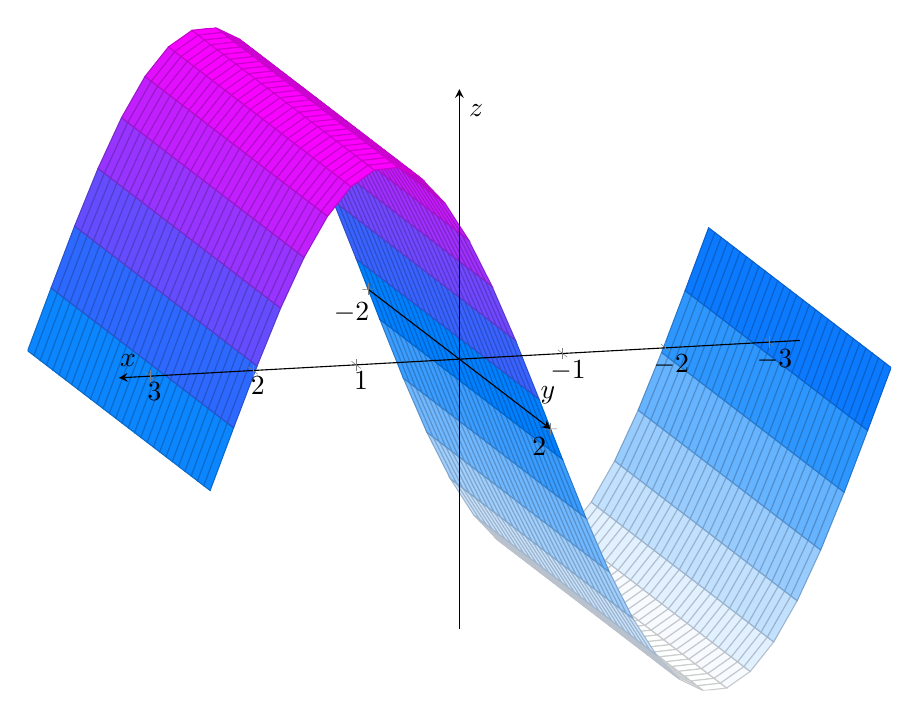
\begin{tikzpicture}
  \begin{axis}[
    view={165}{15},
    axis lines=center,
    xlabel={$x$},
    ylabel={$y$},
    zlabel={$z$},
    domain=-3.3:3.3,
    y domain=-2:2,
    samples=30,
    samples y=30,
    colormap/cool,
    z buffer=sort,
    axis on top,
    scale=1.6,
    ztick={-1,1}
  ]
    \addplot3[surf] {sin(deg(x)};
    \end{axis}
\end{tikzpicture}
\end{center}

\item Hyperbolic paraboloid
\begin{center}
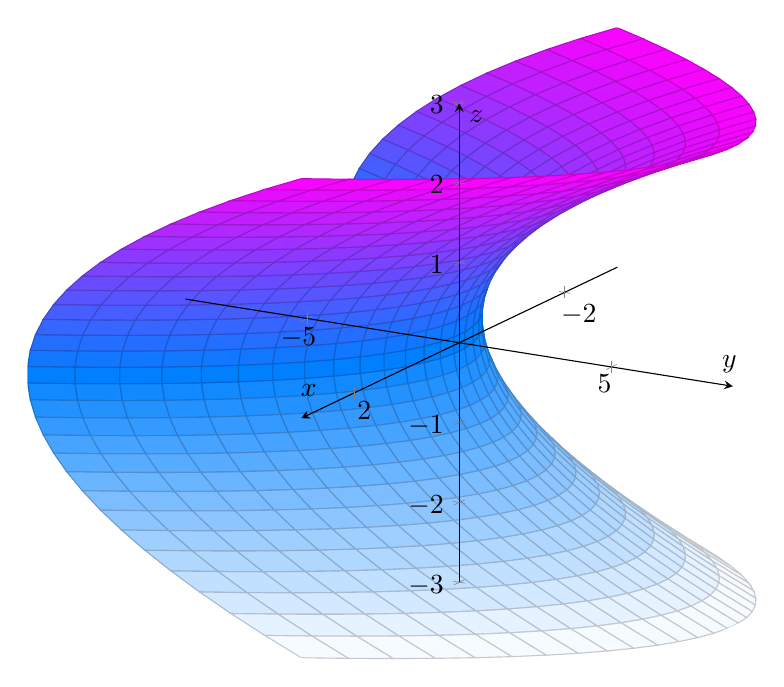
\begin{tikzpicture}
  \begin{axis}[
    view={120}{20},
    axis lines=center,
    xlabel={$x$},
    ylabel={$y$},
    zlabel={$z$},
    domain=-3:3,
    y domain=-3:3,
    samples=30,
    samples y=30,
    colormap/cool,
    z buffer=sort,
    axis on top,
    scale=1.6
  ]
    \addplot3[surf]({x}, {y^2 - x^2}, {y});
  \end{axis}
\end{tikzpicture}
\end{center}
\end{enumerate}

\newpage

\item Apply the Two-Path Test.

\[y=x\implies\lim_{(x,y)\to(0,0)}\frac{xy^2}{x^2+y^4}=\lim_{x\to0}\frac{x^3}{x^2+x^4}=\lim_{x\to0}\frac{x}{1+x^2}=\frac01=0\]
\[x=y^2\implies\lim_{(x,y)\to(0,0)}\frac{xy^2}{x^2+y^4}=\lim_{y\to0}\frac{y^4}{2y^4}=\frac12\]

Since $0\neq\dfrac12$, by the Two-Path Test, the limit does not exist.

\item \begin{enumerate}[leftmargin=*,label=\textbf{\alph*.}]
\item Apply the product rule.

\[\frac\partial{\partial T}\left[\left(P+\frac A{V^2}\right)(V-B)\right]=\frac\partial{\partial T}\left(kT\right)\]

\[\left(\frac{\partial P}{\partial T}-\frac{2A}{V^3}\cdot\frac{\partial V}{\partial T}\right)(V-B)+\left(P+\frac A{V^2}\right)\left(\frac{\partial V}{\partial T}\right)=k\]

\[(V-B)\frac{\partial P}{\partial T}+\frac{\partial V}{\partial T}\left(-\frac{2A}{V^2}+\frac{2AB}{V^3}\right)+\frac{\partial V}{\partial T}\left(P+\frac{A}{V^2}\right)=k\]

\[\boxed{\frac{\partial V}{\partial T}=\frac{k+(B-V)\dfrac{\partial P}{\partial T}}{P+\dfrac{2AB}{V^3}-\dfrac{A}{V^2}}}\]

\item Apply the product rule again.

\[\frac\partial{\partial V}\left[\left(P+\frac A{V^2}\right)(V-B)\right]=\frac\partial{\partial V}\left(kT\right)\]

\[\left(\frac{\partial P}{\partial V}-\frac{2A}{V^3}\right)(V-B)+\left(P+\frac A{V^2}\right)\cdot1=k\frac{\partial T}{\partial V}\]

\[(V-B)\frac{\partial P}{\partial V}-\frac{2A}{V^2}+\frac{2AB}{V^3}=k\frac{\partial T}{\partial V}-P-\frac A{V^2}\]

\[\boxed{\frac{\partial P}{\partial V}=\frac{k\dfrac{\partial T}{\partial V}-P+\dfrac A{V^2}-\dfrac{2AB}{V^3}}{V-B}}\]

\end{enumerate}

\item $z=z(x,y),\:x=x(t)$ and $y=y(t)$. Apply the chain rule.
\begin{align*}\frac{dz}{dt}&=\frac{\partial z}{\partial x}\cdot\frac{dx}{dt}+\frac{\partial z}{\partial y}\cdot\frac{dy}{dt}=(2x-y)(-\sin t)+(2y-x)(\cos t)\\\\&=(2\cos t-\sin t)(-\sin t)+(2\sin t-\cos t)(\cos t)=\sin^2t-\cos^2t=-\cos2t\end{align*}

The result is then

\[\left.\frac{dz}{dt}\right|_{t=0}=-\cos0=\boxed{-1}\]

\item Let $f(x,y,z)=x^2+y^2-z=0$ and $g(x,y,z)=2x^2+2y^2+z^2=8$ be level surfaces. The tangent line is perpendicular to both $\nabla f$ and $\nabla g$ at $P$.

\[\nabla f=\left\langle2x,2y,-1\right\rangle,\qquad\nabla g=\left\langle4x,4y,2z\right\rangle\]
\[\nabla f(P)=\left\langle-2,2,-1\right\rangle,\qquad\nabla g(P)=\left\langle-4,4,4\right\rangle\]
\begin{align*}\mathbf{T}&=\nabla f\times\nabla g=\left|\begin{array}{ccc}
\mathbf{i}&\mathbf{j}&\mathbf{k}\\
-2&2&-1\\
-4&4&4
\end{array}\right|=\mathbf{i}\left|\begin{array}{cc}
2&-1\\4&4
\end{array}\right|-\mathbf{j}\left|\begin{array}{cc}
-2&-1\\-4&4
\end{array}\right|+\mathbf{k}\left|\begin{array}{cc}
-2&2\\-4&4
\end{array}\right|\\\\&=(2\cdot4-4\cdot(-1))\mathbf{i}-(-2\cdot4-(-4)\cdot(-1))\mathbf{j}+(-2\cdot4-2\cdot(-4))\mathbf{k}=12\mathbf i+12\mathbf j\end{align*}

The parametric equations for the tangent line is
\[\boxed{\left.\begin{array}{l}
x=-1+12t\\
y=1+12t\\
z=2
\end{array}\right\}\quad t\in\mathbb{R}}\]

\end{enumerate}

\newpage
\stepcounter{subsection}
\phantomsection
\addcontentsline{toc}{subsection}{\protect\numberline{\thesubsection}Midterm - Spring 2023 Solutions}

\fancyhead[R]{\textit{2022-2023 Spring Midterm}}

%Last update: 25/08/2025 23:50

\begin{enumerate}[leftmargin=*,label=\textbf{\arabic*.}]
\item \begin{enumerate}[leftmargin=*,label=\textbf{\alph*.}]
\item Hyperboloid of one sheet
\begin{center}
\begin{tikzpicture}
  \begin{axis}[
  title={Plane $x=0$},
    xlabel=$y$, ylabel=$z$,
    xtick=\empty, ytick=\empty,
    samples=50,
    axis lines=middle,
    clip=true,
    scale=1,
    enlargelimits=true
    ]
    \addplot[domain=-5:-2, blue] {sqrt(x^2/4-1)};
    \addplot[domain=2:5, blue] {sqrt(x^2/4-1)};
    \addplot[domain=-5:-2, blue] {-sqrt(x^2/4-1)};
    \addplot[domain=2:5, blue] {-sqrt(x^2/4-1)};

    \node[blue] at (2.1,-2) {$\dfrac{y^2}4-z^2=1$};
  \end{axis}
\end{tikzpicture}\hspace{1em}
\begin{tikzpicture}
  \begin{axis}[
  title={Plane $y=0$},
    xlabel=$x$, ylabel=$z$,
    xtick=\empty, ytick=\empty,
    samples=50,
    axis lines=middle,
    clip=true,
    scale=1,
    enlargelimits=true
    ]
    \addplot[domain=-8:-4, red] {sqrt(x^2/16-1)};
    \addplot[domain=4:8, red] {sqrt(x^2/16-1)};
    \addplot[domain=-8:-4, red] {-sqrt(x^2/16-1)};
    \addplot[domain=4:8, red] {-sqrt(x^2/16-1)};

    \node[red] at (3.5,-1.5) {$\dfrac{x^2}{16}-z^2=1$};
  \end{axis}
\end{tikzpicture}

\begin{tikzpicture}
  \begin{axis}[
  title={Plane $z=0$},
  axis equal image,
    xlabel=$x$, ylabel=$y$,
    xtick=\empty, ytick=\empty,
    samples=200,
    axis lines=middle,
    clip=true,
    scale=1,
    enlargelimits=true
    ]
    \addplot[domain=-4:4, orange] {4*sqrt(1-x^2/16)};
    \addplot[domain=-4:4, orange] {-4*sqrt(1-x^2/16)};

    \node[orange] at (1.9,1.1) {\small $\dfrac{x^2}{16}+\dfrac{y^2}4=1$};
  \end{axis}
\end{tikzpicture}\hspace{1em}
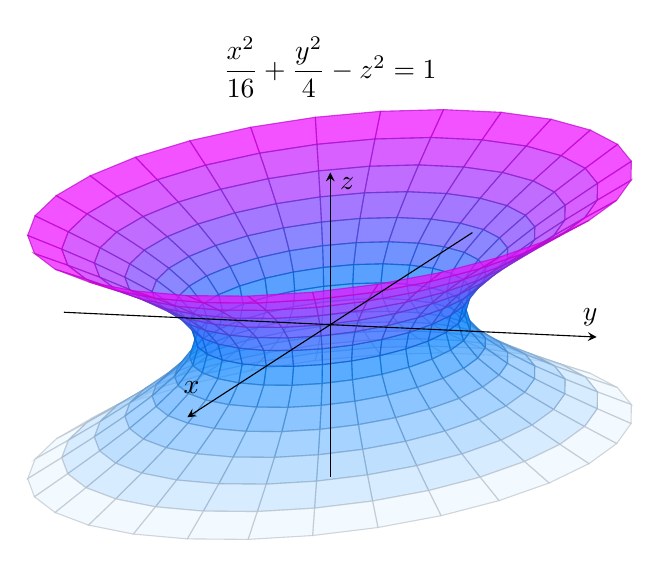
\begin{tikzpicture}
  \begin{axis}[
    title={$\dfrac{x^2}{16}+\dfrac{y^2}4-z^2=1$},
    title style={yshift=-20pt},
      view={105}{10},
      axis lines=center,
      axis equal image,
      xlabel={$x$},
      ylabel={$y$},
      zlabel={$z$},
      domain=0:2*pi,
      y domain=-2:2,
      samples=30,
      samples y=15,
      zmin=-2.5, zmax=2.5,
      colormap/cool,
      axis on top,
      scale=2.5,
      xtick=\empty, ytick=\empty, ztick=\empty,
      z buffer=sort,
    ]
    \addplot3[
      surf,
      opacity=0.7
    ]
    ( {4*sqrt(1+y^2)*cos(deg(x))},
      {2*sqrt(1+y^2)*sin(deg(x))},
      {y} );
  \end{axis}
\end{tikzpicture}
\end{center}

\item Paraboloid
\begin{center}
\begin{tikzpicture}
  \begin{axis}[
  title={Plane $x=0$},
    xlabel=$y$, ylabel=$z$,
    xtick=\empty, ytick=\empty,
    samples=50,
    axis lines=middle,
    clip=true,
    scale=1,
    enlargelimits=true
    ]
    \addplot[domain=-5:5, blue] {x^2/4-6};

    \node[blue] at (1.9,-1.8) {$z=\dfrac{y^2}4-6$};
  \end{axis}
\end{tikzpicture}\hspace{1em}
\begin{tikzpicture}
  \begin{axis}[
  title={Plane $y=0$},
    xlabel=$x$, ylabel=$z$,
    xtick=\empty, ytick=\empty,
    samples=50,
    axis lines=middle,
    clip=true,
    scale=1,
    enlargelimits=true
    ]
    \addplot[domain=-5:5, red] {x^2/4-6};

    \node[red] at (1.9,-1.8) {$z=\dfrac{x^2}4-6$};
  \end{axis}
\end{tikzpicture}

\begin{tikzpicture}
  \begin{axis}[
  title={Plane $z=0$},
  axis equal image,
    xlabel=$x$, ylabel=$y$,
    xtick=\empty, ytick=\empty,
    samples=300,
    axis lines=middle,
    clip=true,
    scale=1,
    enlargelimits=true
    ]
    \addplot[domain=-2*sqrt(6):2*sqrt(6), orange] {sqrt(24-x^2)};
    \addplot[domain=-2*sqrt(6):2*sqrt(6), orange] {-sqrt(24-x^2)};

    \node[orange] at (2.4,0.8) {\small $y^2=24-x^2$};
  \end{axis}
\end{tikzpicture}\hspace{1em}
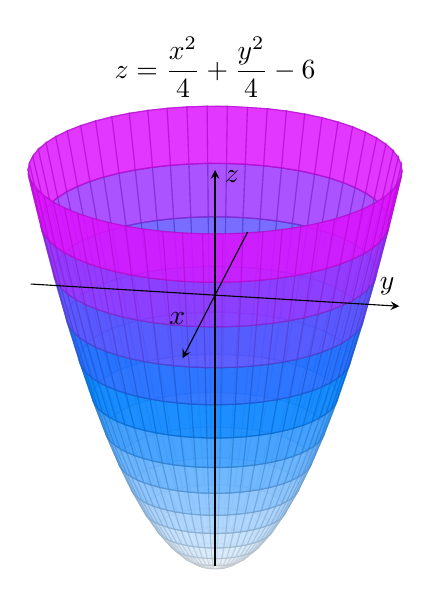
\begin{tikzpicture}
  \begin{axis}[
    title={$\displaystyle z=\frac{x^2}4+\frac{y^2}4-6$},
    title style={yshift=-10pt},
      view={100}{20},
      axis lines=center,
      axis equal image,
      xlabel={$x$},
      ylabel={$y$},
      zlabel={$z$},
      domain=0:2*pi,
      y domain=-2.25:2.25,
      samples=30,
      samples y=30,
      colormap/cool,
      axis on top,
      scale=1.5,
      xtick=\empty, ytick=\empty, ztick=\empty,
      z buffer=sort,
    ]
    \addplot3[
      surf,
      opacity=0.6
    ]
    ( {y*cos(deg(x))},
      {y*sin(deg(x))},
      {y^2-2*sqrt(3)} );
  \end{axis}
\end{tikzpicture}
\end{center}
\end{enumerate}

\item Apply the Two-Path Test.
\[x=y\implies\lim_{(x,y)\to(0,0)}\frac{y^3\sqrt x}{2\left(x^2+y^4\right)}=\lim_{x\to0}\frac{x^{7/2}}{2\left(x^2+x^4\right)}=\lim_{x\to0}\frac{x^{3/2}}{2\left(1+x^2\right)}=\frac02=0\]
\[x=y^2\implies\lim_{(x,y)\to(0,0)}\frac{y^3\sqrt x}{2\left(x^2+y^4\right)}=\lim_{y\to0}\frac{y^4}{4y^4}=\lim_{y\to0}\frac14=\frac14\]

Since $0\neq\dfrac14$, by the Two-Path Test, the limit does not exist.

\item Let $f(x,y,z)=xz^2-2xy+y^2=2$ and $g(x,y,z)=xz-x^2y+z^2=1$ be the level surfaces. The cross product of the gradient of these functions give us the vector that is parallel to the line of intersection. Compute the gradients.
\[\nabla f=\left\langle z^2-2y,\:-2x+2y,\:2xz\right\rangle,\quad \nabla g=\left\langle z-2xy,\:-x^2,\: x+2z\right\rangle\]
\[\nabla f\,|_{\left(0,\,\sqrt2,\,1\right)}=\left\langle1-2\sqrt2,\:2\sqrt2,\:0\right\rangle,\quad \nabla g\,|_{\left(0,\,\sqrt2,\,1\right)}=\left\langle1,\:0,\:2\right\rangle\]

Find the cross product.
\begin{align*}\mathbf{n}&=\nabla f\times \nabla g=\left|\begin{array}{ccc}
\mathbf{i}&\mathbf{j}&\mathbf{k}\\
1-2\sqrt2&2\sqrt2&0\\
1&0&2
\end{array}\right|\\[1em]&=\mathbf{i}\left|\begin{array}{cc}
2\sqrt2&0\\0&2
\end{array}\right|-\mathbf{j}\left|\begin{array}{cc}
1-2\sqrt2&0\\1&2
\end{array}\right|+\mathbf{k}\left|\begin{array}{cc}
1-2\sqrt2&2\sqrt2\\1&0
\end{array}\right|\\[1em]&=\left(2\sqrt2\cdot2-0\cdot0\right)\mathbf{i}-\left[\left(1-2\sqrt2\right)\cdot2-0\cdot1\right]\mathbf{j}+\left[\left(1-2\sqrt2\right)\cdot0-2\sqrt2\cdot1\right)\mathbf{k}\\[1em]&=4\sqrt2\,\mathbf{i}+\left(4\sqrt2-2\right)\,\mathbf{j}+-2\sqrt2\,\mathbf{k}\end{align*}

The line of intersection is the normal line of the plane. Therefore, $\mathbf n$ is the normal vector of the plane. The equation of the plane with the normal vector $\mathbf n$ and containing the point $P(x_0,y_0,z_0)$ is
\[n_1(x-x_0)+n_2(y-y_0)+n_3(z-z_0)=0\]

Therefore, the equation for this plane is
\[4\sqrt2(x-0)+\left(4\sqrt2-2\right)(y-1)-2\sqrt2(z-2)=0\]
\[\boxed{2x\sqrt2+y\left(2\sqrt2-1\right)-z\sqrt2+1=0}\]

\item Apply the chain rule.
\[\frac{\partial w}{\partial s}=\frac{\partial w}{\partial x}\cdot\frac{\partial x}{\partial s}+\frac{\partial w}{\partial y}\cdot\frac{\partial y}{\partial s}+\frac{\partial w}{\partial z}\cdot\frac{\partial z}{\partial s}\]

Compute the partial derivatives.
\[\frac{\partial w}{\partial x}=y\ln\left(1+\sqrt{x^2+y^2}\right)+xy\cdot\frac1{1+\sqrt{x^2+y^2}}\cdot\left(\frac{x}{\sqrt{x^2+y^2}}\right)+z\]
\[\frac{\partial w}{\partial y}=x\ln\left(1+\sqrt{x^2+y^2}\right)+xy\cdot\frac1{1+\sqrt{x^2+y^2}}\cdot\left(\frac{y}{\sqrt{x^2+y^2}}\right),\quad \frac{\partial w}{\partial z}=x\]
\[\frac{\partial x}{\partial s}=1,\quad\frac{\partial y}{\partial s}={e}^s,\quad\frac{\partial z}{\partial s}=\frac{2s}{s^2+t}\]

\begin{align*}\frac{\partial w}{\partial s}=&\left[y\ln\left(1+\sqrt{x^2+y^2}\right)+xy\cdot\frac1{1+\sqrt{x^2+y^2}}\cdot\left(\frac{x}{\sqrt{x^2+y^2}}\right)+z\right]\cdot1\\[1em]&+\left[x\ln\left(1+\sqrt{x^2+y^2}\right)+xy\cdot\frac1{1+\sqrt{x^2+y^2}}\cdot\left(\frac{y}{\sqrt{x^2+y^2}}\right)\right]\cdot{e}^s+\frac{2xs}{s^2+t}\end{align*}

Write in terms of $s$ and $t$ rigorously.
\[\boxed{\begin{array}{ll}\dfrac{\partial w}{\partial s}=&
{e}^s\ln\left(1+\sqrt{(t+s)^2+{e}^{2s}}\right)+\dfrac{(t+s)^2\cdot{e}^s}{\sqrt{(t+s)^2+{e}^{2s}}+(t+s)^2+{e}^{2s}}+\ln\left(s^2+t\right)\\[1em]&+(t+s){e}^s\ln\left(1+\sqrt{(t+s)^2+{e}^{2s}}\right)+\dfrac{(t+s)\cdot{e}^{3s}}{\sqrt{(t+s)^2+{e}^{2s}}+(t+s)^2+{e}^{2s}}\\[1em]&+\dfrac{2s(t+s)}{s^2+t}
\end{array}}\]

\item Let $f(x,y)=\tan\left(xy^2\right)$. The total differential of $f$ is
\[df=f_x\,dx+f_y\,dy=\sec^2\left(xy^2\right)\cdot y^2\,dx+\sec^2\left(xy^2\right)\cdot2xy\,dy\]

Since $x=0.97\approx1$ and $y=2.05\approx2$, we may approximate the value of \linebreak $\tan\left(0.97\cdot2.05^2\right)$ near $\tan\left(1\cdot 2^2\right)=\tan4$. Take $x=1,\:y=2,\:dx=0.97-1=-0.03,\:dy=2.05-2=0.05$.
\[df=\sec^24\cdot4\cdot(-0.03)+\sec^24\cdot4\cdot(0.05)=0.08\sec^24\]

Since $f(x+\Delta x,\:y+\Delta y)\approx f(x,y)+df$, the value of $\tan\left(0.97\cdot2.05^2\right)$ is approximately
\[\boxed{\tan4+0.08\sec^24}\]

\item The function $f$ has the minimum rate of change if the gradient vector of $f$ and the unit direction vector $\mathbf u$ are antiparallel. That is, they have opposite directions.
\[\nabla f=\left\langle\frac1{2\sqrt{x+yz}},\frac z{2\sqrt{x+yz}},\frac y{2\sqrt{x+yz}}\right\rangle\]
\[\left(\nabla f\cdot \mathbf u\right)_{\text{min}}=\left|\nabla f\right||u|\cos\pi=-|\nabla f|\]
\[\nabla f|_{(1,1,3)}=\left\langle\frac14,\frac34,\frac14\right\rangle\implies-|\nabla f|=-\sqrt{\left(\frac14\right)^2+\left(\frac34\right)^2+\left(\frac14\right)^2}=-\frac{\sqrt{11}}4\]

Since $\mathbf u$ has the opposite direction to that of the gradient, we may also find the components of $\mathbf u$.
\[\mathbf{u}=-\frac{\nabla f}{|\nabla f|}=-\frac{\left\langle\frac14,\frac34,\frac14\right\rangle}{\frac{\sqrt{11}}4}=\left\langle-\frac1{\sqrt{11}},-\frac3{\sqrt{11}},-\frac1{\sqrt{11}}\right\rangle\]
\[\boxed{\text{The minimum rate of change: }{-\frac{\sqrt{11}}4},\text{ direction vector:}\left\langle-\frac1{\sqrt{11}},-\frac3{\sqrt{11}},-\frac1{\sqrt{11}}\right\rangle}\]

\item $f$ is continuous on a bounded and closed set on $\mathbb R$. By the Extreme Value Theorem, the extrema must exist in the region or on the boundary.

First, determine where $f_x=f_y=0$ to find the critical points.
\[f_x=2x-y,\quad f_y=1-x\]
\[f_x=f_y=0\implies2x-y=0,\quad1-x=0\implies x=1,\quad y=2\]
\[f(1,2)=5\]

Take a look at the boundary. From $(0,0)$ to $(4,0)$, we have $y=0$.
\[y=0\implies f(x,0)=x^2+4\quad\rightarrow\quad\frac d{dx}\left(x^2-4\right)=2x=0\implies x=0\]
\[f(0,0)=4\]

From $(0,0)$ to $(0,4)$, we have $x=0$.
\[x=0\implies f(0,y)=y+4\quad\rightarrow\quad\frac d{dy}\left(y+4\right)=1\neq0\]

From $(4,0)$ to $(0,4)$, we have $x=y$.
\[y=4-x\implies f(x,4-x)=x^2+(4-x)-x(4-x)+4=2x^2-5x+8\]

\[\frac d{dx}\left(2x^2-5x+8\right)=4x-5=0\implies x=\frac54,\quad y=\frac{11}4\]
\[f\left(\frac54,\frac{11}4\right)=\frac{39}8\]

We also have $f(0,0)=5,\:f(4,0)=20,\:f(0,4)=8$ from the vertices of the triangular region.

Compare all the values $f(0,0),\:f(1,2),\:f(4,0),\:f(0,4),\:f\left(\frac54,\frac{11}4\right)$.
\[\boxed{\text{Absolute minimum: }f(0,0)=4,\quad \text{absolute maximum: } f(4,0)=20.}\]
\end{enumerate}

\newpage
\stepcounter{subsection}
\phantomsection
\addcontentsline{toc}{subsection}{\protect\numberline{\thesubsection}Midterm - Spring 2024 Solutions}

\newpage
\fancyhead[R]{\textit{2023-2024 Spring Midterm}}

%Last update: 27/08/2025 23:24

\begin{enumerate}[leftmargin=*,label=\textbf{\arabic*.}]
\item \begin{enumerate}[leftmargin=*,label=\textbf{\alph*.}]
\item\leavevmode
\vspace{-1.2em}\begin{center}
\begin{tikzpicture}
  \begin{axis}[
  title={Plane $x=0$},
    xlabel=$y$, ylabel=$z$,
    xtick=\empty, ytick=\empty,
    samples=30,
    axis lines=middle,
    clip=true,
    scale=0.9,
    enlargelimits=true
    ]
    \addplot[domain=-1:0.8, blue] {e^x};

    \node[blue] at (0.5,1) {$z={e}^y$};
  \end{axis}
\end{tikzpicture}\hspace{1em}
\begin{tikzpicture}
  \begin{axis}[
  title={Plane $y=0$},
    xlabel=$x$, ylabel=$z$,
    xtick=\empty, ytick=\empty,
    axis lines=middle,
    samples=30,
    clip=true,
    ymin=0, ymax=2,
    scale=0.9,
    enlargelimits=true
    ]
    \addplot[domain=-2:2, red, thick] {1};

    \node[red] at (1.5,1.5) {$z=1$};
  \end{axis}
\end{tikzpicture}

\vspace{1em}

\begin{tikzpicture}
  \begin{axis}[
  title={Plane $z=0$ (No intersection)},
  axis equal image,
    xlabel=$x$, ylabel=$y$,
    xtick=\empty, ytick=\empty,
    xmin=-1, xmax=1,
    ymin=-1, ymax=1,
    axis lines=center,
    clip=true,
    scale=0.9,
    enlargelimits=true
    ]
  \end{axis}
\end{tikzpicture}\hspace{1em}
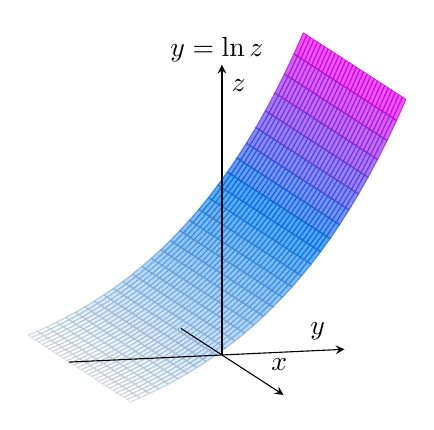
\begin{tikzpicture}
  \begin{axis}[
    title={$y=\ln z$},
    title style={yshift=-20pt},
      view={75}{10},
      axis lines=center,
      axis equal image,
      xlabel={$x$},
      ylabel={$y$},
      zlabel={$z$},
      domain=-1:1.5,
      y domain=-1:0.8,
      samples=30,
      samples y=30,
      colormap/cool,
      axis on top,
      scale=0.9,
      xtick=\empty, ytick=\empty, ztick=\empty,
      z buffer=sort,
    ]
    \addplot3[
      surf,
      opacity=0.7
    ]
    ( {x},
      {y},
      {e^y} );
  \end{axis}
\end{tikzpicture}
\end{center}

\item\leavevmode
\vspace{-1.2em}
\begin{center}
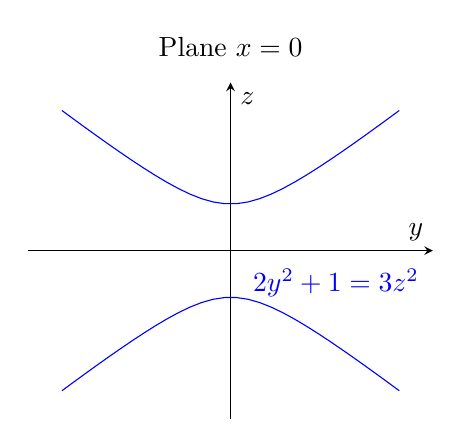
\begin{tikzpicture}
  \begin{axis}[
  title={Plane $x=0$},
    xlabel=$y$, ylabel=$z$,
    xtick=\empty, ytick=\empty,
    samples=30,
    axis lines=middle,
    clip=true,
    scale=0.75,
    enlargelimits=true
    ]
    \addplot[domain=-2:2, blue] {sqrt(2*x^2/3+1/3)};
    \addplot[domain=-2:2, blue] {-sqrt(2*x^2/3+1/3)};
    
    \node[blue] at (1.25,-0.4) {$2y^2+1=3z^2$};
  \end{axis}
\end{tikzpicture}\hspace{1em}
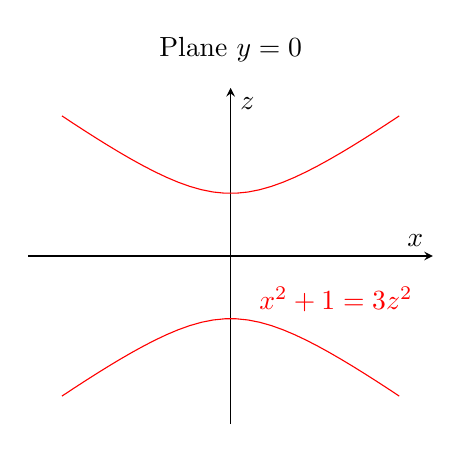
\begin{tikzpicture}
  \begin{axis}[
  title={Plane $y=0$},
    xlabel=$x$, ylabel=$z$,
    xtick=\empty, ytick=\empty,
    samples=30,
    axis lines=middle,
    clip=true,
    scale=0.75,
    enlargelimits=true
    ]
    \addplot[domain=-2:2, red] {sqrt(x^2/3+1/3)};
    \addplot[domain=-2:2, red] {-sqrt(x^2/3+1/3)};
    
    \node[red] at (1.25,-0.4) {$x^2+1=3z^2$};
  \end{axis}
\end{tikzpicture}

\begin{tikzpicture}
  \begin{axis}[
  title={Plane $z=0$ (No intersection)},
  axis equal image,
    xlabel=$x$, ylabel=$y$,
    xtick=\empty, ytick=\empty,
    xmin=-1, xmax=1,
    ymin=-1, ymax=1,
    axis lines=center,
    clip=true,
    scale=0.9,
    enlargelimits=true
    ]
  \end{axis}
\end{tikzpicture}\hspace{1em}
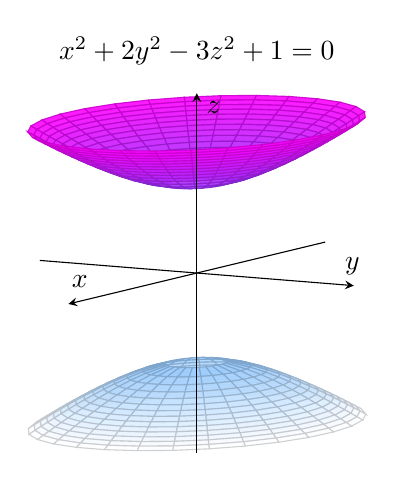
\begin{tikzpicture}
  \begin{axis}[
  title={$x^2+2y^2-3z^2+1=0$},
    title style={yshift=-15pt},
      view={120}{8},
      axis lines=center,
      axis equal image,
      xlabel={$x$},
      ylabel={$y$},
      zlabel={$z$},
      domain=0:2*pi,
      y domain=-2:2,
      samples=30,
      samples y=30,
      colormap/cool,
      axis on top,
      scale=1.3,
      xtick=\empty, ytick=\empty, ztick=\empty,
      z buffer=sort,
      enlargelimits=true,
    ]
    \addplot3[
      surf,
      opacity=0.9
    ]
    ( {sqrt(y)*cos(deg(x))},
      {1/sqrt(2))*sqrt(y)*sin(deg(x))},
      {(1/sqrt(3))*sqrt(y+1)} );
    \addplot3[
      surf,
      opacity=0.9
    ]
    ( {-sqrt(y)*cos(deg(x))},
      {-1/sqrt(2))*sqrt(y)*sin(deg(x))},
      {-(1/sqrt(3))*sqrt(y+1)} );
  \end{axis}
\end{tikzpicture}
\end{center}
\end{enumerate}

\newpage
\item The $\epsilon-\delta$ definition is the formal way of calculating the limit of a function at a point $(x_0,y_0)$. According to the definition, for every $\epsilon>0$, there exists a $\delta$ such that
\[0<\sqrt{(x-x_0)^2+(y-y_0)^2}<\delta\implies\left|f(x,y)-L\right|<\epsilon,\]
where $L$ is the limit.

Then for every $\epsilon>0$, there exists a $\delta$ such that
\[0<\sqrt{x^2+y^2}<\delta\implies\left|2x^2+y^2\right|<\epsilon.\]
\[\left|2x^2+y^2\right|\leq2x^2+y^2\qquad\left[x^2\geq0,\quad y^2\geq0\right]\]
\[2x^2+y^2\leq2x^2+2y^2=2\left(x^2+y^2\right)\leq2\delta^2\qquad\left[\sqrt{x^2+y^2}<\delta\implies  x^2+y^2<\delta^2\right]\]

Let $\delta=\sqrt{\dfrac{\epsilon}2}$.
\[\left|2x^2+y^2\right|\leq2\left(x^2+y^2\right)<2\cdot\left(\sqrt{\frac{\epsilon}2}\right)^2=2\cdot\frac{\epsilon}2=\epsilon\]

This shows that the limit is equal to $0$.

\item The coefficients of the parametrization variables have the same ratio. That is, they are parallel. Choose $P_1(3,3,3)$ on $l_1$ and $P_2(1,2,1)$ on $l_2$. The cross product of $\mathbf u=\left\langle3,-1,2\right\rangle$, which is parallel to the lines, and the vector $\mathbf v$ joining $P_1$ and $P_2$, where $\mathbf w=\left\langle3-1,\,3-2,\,3-1\right\rangle=\left\langle2,1,2\right\rangle$, gives us the normal of the plane.
\begin{align*}\mathbf n&=\mathbf{u}\times\mathbf{v}=\left|\begin{array}{ccc}
\mathbf{i}&\mathbf{j}&\mathbf{k}\\
3&-1&2\\
2&1&2
\end{array}\right|=\mathbf{i}\left|\begin{array}{cc}
-1&2\\1&2
\end{array}\right|-\mathbf{j}\left|\begin{array}{cc}
3&2\\2&2
\end{array}\right|+\mathbf{k}\left|\begin{array}{cc}
3&-1\\2&1
\end{array}\right|\\[1em]&=(-1\cdot2-1\cdot2)\mathbf{i}-(3\cdot2-2\cdot2)\mathbf{j}+(3\cdot1-2\cdot(-1))\mathbf{k}=-4\mathbf i-2\mathbf j+5\mathbf k\end{align*}

Using the definition $\mathbf{n}\cdot\overrightarrow{PP_1}=0$, where $P$ is a point on the plane, the equation of the plane is
\begin{align*}\mathbf{n}\cdot\overrightarrow{PP_1}=0&\implies\left\langle-4,-2,5\right\rangle\cdot\left\langle x-3,\,y-3,\,z-3\right\rangle=0\\[1em]&\implies-4(x-3)-2(y-3)+5(z-3)=0\implies\boxed{-4x-2y+5z+3=0}\end{align*}

\item \begin{enumerate}[leftmargin=*,label=\textbf{\alph*.}]
\item Use the definition of the partial derivative.
\begin{align*}f_x|_{(0,0)}&=\lim_{h\to0}\frac{f(0+h,0)-f(0,0)}h=\lim_{h\to0}\frac{\dfrac{(0+h)^2\cdot{e}^{(0+h)^2+0}}{(0+h)^2+0^2}}{h}=\lim_{h\to0}\frac{{e}^{h^2}}{h}\\[1em]&=\infty\:(f_x\:\text{does not exist})\end{align*}
\[f_y|_{(0,0)}=\lim_{h\to0}\frac{f(0,0+h)-f(0,0)}h=\lim_{h\to0}\frac{\dfrac{0^2\cdot{e}^{0^2+(0+h)}}{0^2+(0+h)^2}}{h}=\lim_{h\to0}\frac{0}{h}=0\]

\item $f_y$ is a finite number. However, since $f_x$ does not exist, $f$ is not differentiable at $(0,0)$.
\end{enumerate}

\item $u$ and $v$ are functions of $x$ and $y$. $x$ and $y$ are functions of $r$ and $\theta$. Use the chain rule.
\[\frac{\partial u}{\partial r}=\frac{\partial u}{\partial x}\cdot\frac{\partial x}{\partial r}+\frac{\partial u}{\partial y}\cdot\frac{\partial y}{\partial r}=u_x\cdot\cos\theta+u_y\cdot\sin\theta=v_y\cos\theta-v_x\sin\theta\]
\[\frac{\partial v}{\partial\theta}=\frac{\partial v}{\partial x}\cdot\frac{\partial x}{\partial\theta}+\frac{\partial v}{\partial y}\cdot\frac{\partial y}{\partial\theta}\implies\frac1r\frac{\partial v}{\partial\theta}=\frac1r\left(-v_x\cdot r\sin\theta+v_y\cdot r\cos\theta\right)=-v_x\sin\theta+v_y\cos\theta\]
\[\frac{\partial u}{\partial r}=-v_x\sin\theta+v_y\cos\theta=\frac1r\frac{\partial v}{\partial\theta}\]
\[\frac{\partial v}{\partial r}=\frac{\partial v}{\partial x}\cdot\frac{\partial x}{\partial r}+\frac{\partial v}{\partial y}\cdot\frac{\partial y}{\partial r}=v_x\cdot\cos\theta+v_y\cdot\sin\theta=-u_y\cos\theta+u_x\sin\theta\]
\[\frac{\partial u}{\partial\theta}=\frac{\partial u}{\partial x}\cdot\frac{\partial x}{\partial\theta}+\frac{\partial u}{\partial y}\cdot\frac{\partial y}{\partial\theta}\implies-\frac1r\frac{\partial u}{\partial\theta}=-\frac1r\left(-u_x r\sin\theta+u_y r\cos\theta\right)=u_x\sin\theta-u_y\cos\theta\]
\[\frac{\partial v}{\partial r}=u_x\sin\theta-u_y\cos\theta=-\frac1r\frac{\partial u}{\partial \theta}\]

\item The function $f$ has the maximum rate of change if the gradient vector of $f$ and the unit direction vector $\mathbf u$ are in the same direction. Apply the quotient rule to compute the gradient of $f$.
\[\nabla f=\left\langle\frac{\left(2^{xy}\cdot y\cdot\ln2\right)\cdot x-2^{xy}\cdot(1)}{x^2},\,2^{xy}\cdot\ln2\right\rangle=\left\langle\frac{2^{xy}\left(yx\ln2-1\right)}{x^2},\,2^{xy}\cdot\ln2\right\rangle\]
\[\left(\nabla f\cdot\mathbf u\right)_{\text{max}}=\left|\nabla f\right||u|\cos0=|\nabla f|\]
\begin{align*}\nabla f|_{(1,1)}&=\left\langle2\ln2-2,\,2\ln2\right\rangle\implies|\nabla f|=\sqrt{\left(2\ln2-2\right)^2+\left(2\ln2\right)^2}\\[1em]&=2\sqrt{2\ln^22-2\ln2+1}\end{align*}

The unit direction vector $u$ is
\[\mathbf{u}=\frac{\nabla f}{|\nabla f|}=\frac{\left\langle2\ln2-2,\,2\ln2\right\rangle}{2\sqrt{2\ln^22-2\ln2+1}}=\left\langle\frac{\ln2-1}{\sqrt{2\ln^22-2\ln2+1}},\frac{\ln2}{\sqrt{2\ln^22-2\ln2+1}}\right\rangle\]
\[\boxed{\begin{array}{c}\text{The maximum rate of change: }{2\sqrt{2\ln^22-2\ln2+1}}\\[1em]\text{The direction vector:}\left\langle\dfrac{\ln2-1}{\sqrt{2\ln^22-2\ln2+1}},\dfrac{\ln2}{\sqrt{2\ln^22-2\ln2+1}}\right\rangle\end{array}}\]

\item Apply the chain rule.
\begin{align*}f_x&=(y+1)\left[1\cdot(x-y+3)+(x-1)\cdot1\right]=(y+1)(2x-y+2)\\[1em]&=2xy-y^2+2y+2x-y+2=-y^2+y+2xy+2x+2\end{align*}
\begin{align*}f_y&=(x-1)\left[1\cdot(x-y+3)+(y+1)\cdot(-1)\right]=(x-1)(x-2y+2)\\[1em]&=x^2-2xy+2x-x+2y-2=x^2-2xy+x+2y-2\end{align*}

The critical points occur where one of the partial derivatives does not exist or $f_x=f_y=0$. $f_x$ and $f_y$ are continuous everywhere. Therefore, we may simply determine where $f_x=f_y=0$.

\begin{align*}f_x=f_y=0&\implies\left.\begin{array}{r}
2xy-y^2+2y+2x-y+2=0\\
x^2-2xy+x+2y-2=0
\end{array}\right\}\quad x^2-y^2+3(x+y)=0\\[1em]&\implies(x-y)(x+y)+3(x+y)=0\implies(x-y+3)(x+y)=0\end{align*}

We have two cases: $x+3=y$ or $x=-y$.
\begin{flalign*}\textit{Case I}:x=-y&\implies-y^2-2y^2+y-2y+2=0\implies -3y^2-y+2=0\\[1em]&\implies
(2-3y)(y+1)=0\implies y_1=\frac23,\:y_2=-1&\end{flalign*}
\[y_1=\frac23\implies x_1=-\frac23\qquad y_2=-1\implies x_2=1\]
\begin{flalign*}\textit{Case II}:x+3=y&\implies-(x+3)^2+2x(x+3)+x+3+2x+2=0\\[1em]&\implies-x^2-6x-9+2x^2+6x+3x+5=0\\[1em]&\implies x^2+3x-4=0&\end{flalign*}
\begin{flalign*}x_{3,4}=\frac{-3\pm\sqrt{9-4\cdot1\cdot(-4)}}{2\cdot1}=\frac{-3\pm5}2&\implies x_3=-4,\:x_4=1\\&\implies y_3=-1,\:y_4=4\end{flalign*}

To classify these four critical points, apply the Second Derivative Test.
\[f_{xx}=2y+2,\quad f_{xy}=f_{yx}=2x-2y+1,\quad f_{yy}=-2x+2\]
\begin{flalign*}\left(-\frac23,\frac23\right)\rightarrow\left\{\:\begin{array}{l}
f_{xx}=\dfrac{10}3,\quad f_{xy}=-\dfrac53 ,\quad f_{yy}=\dfrac{10}3\\[1em]
\left|\begin{array}{cc}
\dfrac{10}3&-\dfrac{10}3\\[1em]
-\dfrac53 & \dfrac{10}3
\end{array}\right|=\dfrac{10}3\cdot\dfrac{10}3-\left(-\dfrac53\right)\cdot\left(-\dfrac53\right)=\dfrac{25}3,\quad f_{xx}=\dfrac{10}3>0
\end{array}\right.&&\end{flalign*}
\begin{flalign*}\left(1,-1\right)\rightarrow\left\{\:\begin{array}{l}
f_{xx}=0,\quad f_{xy}=5,\quad f_{yy}=0\\[1em]
\left|\begin{array}{cc}
0 & 5\\
5 & 0
\end{array}\right|=0\cdot0-5\cdot5=-25<0
\end{array}\right.&&\end{flalign*}
\begin{flalign*}\left(-4,-1\right)\rightarrow\left\{\:\begin{array}{l}
f_{xx}=0,\quad f_{xy}=-5,\quad f_{yy}=10\\[1em]
\left|\begin{array}{cc}
0 & -5\\
-5 & 10
\end{array}\right|=0\cdot10-(-5)\cdot(-5)=-25<0
\end{array}\right.&&\end{flalign*}
\begin{flalign*}\left(1,4\right)\rightarrow\left\{\:\begin{array}{l}
f_{xx}=10,\quad f_{xy}=5,\quad f_{yy}=0\\[1em]
\left|\begin{array}{cc}
10 & 5\\
5 & 0
\end{array}\right|=10\cdot0-5\cdot5=-25<0
\end{array}\right.&&\end{flalign*}

\[\boxed{\begin{array}{c}\text{A local minimum occurs at }\left(-\dfrac23,\dfrac23\right).\\\text{ Saddle points occur at } (1,-1), (-4,-1),\:\text{and}\:(1,4).\end{array}}\]

\end{enumerate}

\newpage
\stepcounter{subsection}
\phantomsection
\addcontentsline{toc}{subsection}{\protect\numberline{\thesubsection}Midterm - Spring 2025 Solutions}

\fancyhead[R]{\textit{2024-2025 Spring Midterm}}

%Last update: 29/08/2025 01:59

\begin{enumerate}[leftmargin=*,label=\textbf{\arabic*.}]
\item \begin{enumerate}[leftmargin=*,label=\textbf{\alph*.}]
\item Determine whether the graph is symmetric about the $x$-axis.
\[(r,\theta)\rightarrow r=2\cos(3\theta),\qquad (r,-\theta)\rightarrow r=2\cos(-3\theta)=2\cos(3\theta)\]

$(r,\theta)$ is on the graph, and the graph is symmetric about the $x$-axis. Determine whether the graph is symmetric about the origin.
\[(r,\theta)\rightarrow r=2\cos(3\theta),\qquad (r,\theta+\pi)\rightarrow r=2\cos(-3(\theta+\pi))=-2\cos(3\theta)\]

$(r,\theta+\pi)$ is not on the graph, and the graph is not symmetric about the origin. Determine whether the graph is symmetric about the $y$-axis.
\[(r,\theta)\rightarrow r=2\cos(3\theta),\qquad (r,\theta-\pi)\rightarrow r=2\cos(-3(\theta-\pi))=-2\cos(3\theta)\]

$(r,\theta-\pi)$ is not on the graph, and the graph is not symmetric about the $y$-axis. 

\begin{center}
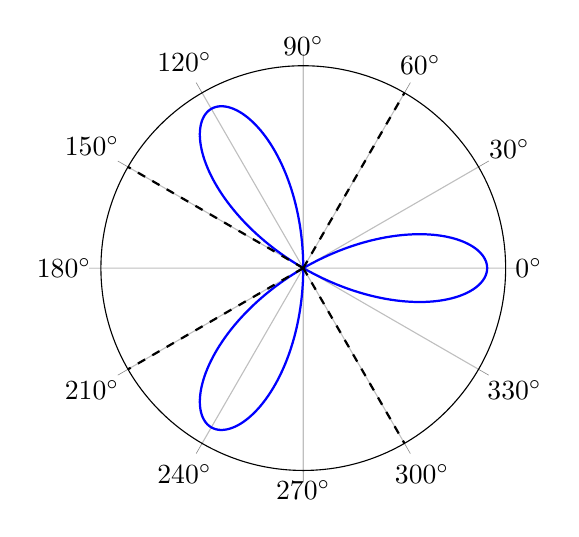
\begin{tikzpicture}
  \begin{polaraxis}[ytick=\empty, axis y line=none, xticklabel=$\pgfmathprintnumber{\tick}^\circ$,      scale=0.75,]
    \addplot [
      domain=0:2*pi,
      samples=300,
      thick,
      blue,
      data cs=polarrad,
    ] {2*cos(deg(3*x))};

    \draw[black, thick, dashed] (axis cs: 60,0) -- (axis cs: 60,2.5);
    \draw[black, thick, dashed] (axis cs: -60,0) -- (axis cs: -60,2.5);
    \draw[black, thick, dashed] (axis cs: 150,0) -- (axis cs: 150,2.5);
    \draw[black, thick, dashed] (axis cs: 210,0) -- (axis cs: 210,2.5);

  \end{polaraxis}
\end{tikzpicture}
\end{center}

\item It is sufficient to calculate the area of the upper half of the leaf right to the $y$-axis and multiply the result by six.

\begin{center}
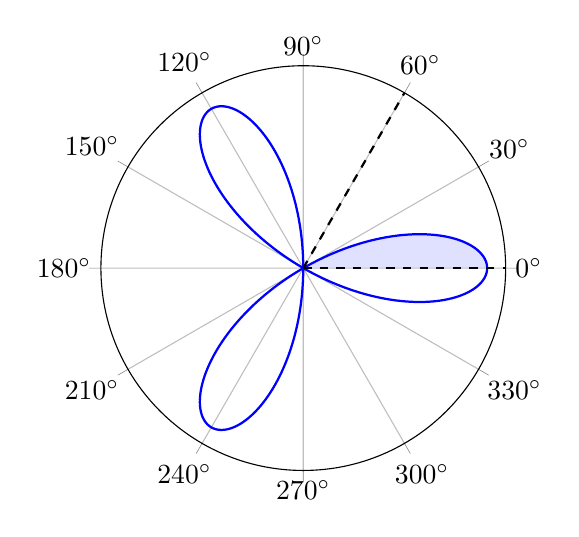
\begin{tikzpicture}
  \begin{polaraxis}[ytick=\empty, axis y line=none, xticklabel=$\pgfmathprintnumber{\tick}^\circ$,      scale=0.75,]
    \addplot [
      domain=0:2*pi,
      samples=300,
      thick,
      blue,
      data cs=polarrad,
    ] {2*cos(deg(3*x))};
    
    \addplot [
      domain=0:pi/6,
      draw=none,
      data cs=polarrad,
      name path=B
    ] {2*cos(deg(3*x))};
    
    \addplot [
      domain=0:pi/6,
      draw=none,
      data cs=polarrad,
      name path=A
    ] {0};
    
    \addplot [
      blue!20,
      fill opacity=0.6,
    ] fill between[of=A and B];

    \draw[black, thick, dashed] (axis cs: 60,0) -- (axis cs: 60,2.5);
    \draw[black, thick, dashed] (axis cs: 0,0) -- (axis cs: 0,2.5);

  \end{polaraxis}
\end{tikzpicture}
\end{center}
\begin{align*}\frac12\int_0^{\pi/6}\left(2\cos(3\theta)\right)^2\,d\theta&=\frac12\int_0^{\pi/6}4\cos^2(3\theta)\,d\theta=2\int_0^{\pi/6}\frac{1-\cos(6\theta)}2\,d\theta\\[1em]&=\left.\theta-\frac{\sin(6\theta)}6\right|_0^{\pi/6}=\frac\pi6\end{align*}

The area is then
\[\text{Area}=6\cdot\frac\pi6=\boxed{\pi}\]

\end{enumerate}

\item \begin{enumerate}[leftmargin=*,label=\textbf{\alph*.}]
\item Multiply each side by $r$.
\[r=2\sin\theta+2\cos\theta\implies r^2=2r\sin\theta+2r\cos\theta\]

Using the equations $x=r\cos\theta$ and $y=r\sin\theta$, we get
\begin{align*}x^2+y^2=2x+2y&\implies x^2-2x+y^2+2y=0\implies x^2-2x+1+y^2-2y+1=2\\[1em]&\implies(x-1)^2+(y-1)^2=\left(\sqrt2\right)^2\end{align*}

This is a circle with radius $\sqrt2$ centered at $(1,1)$.
\begin{center}
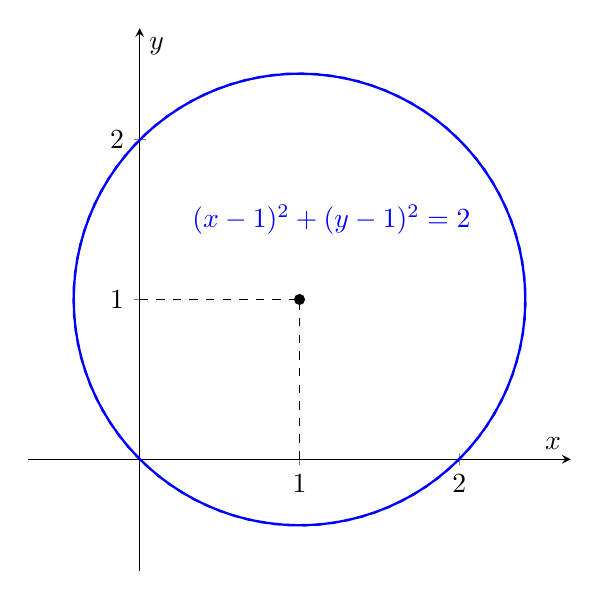
\begin{tikzpicture}
  \begin{axis}[
      axis lines = center,
      xlabel = {$x$},
      ylabel = {$y$},
      samples=100,
      xtick={1,2}, ytick={1,2},
      scale=1.21,
      axis equal image,
      enlargelimits=true,
    ]
    
    \addplot[blue, thick, domain=0:360] ({(2*sin(x)+2*cos(x))*cos(x)}, {(2*sin(x)+2*cos(x))*sin(x)});
    \fill (axis cs:1,1) circle (2pt);
    \node[blue] at (1.2,1.5) {$(x-1)^2+(y-1)^2=2$};
    \draw[dashed](1,0)--(1,1); \draw[dashed](0,1)--(1,1);
  \end{axis}
\end{tikzpicture}
\end{center}

\item Rearrange the equation.
\[r=\tan\theta\sec\theta=\frac{\sin\theta}{\cos^2\theta}\implies r\cos^2\theta=\sin\theta\implies r^2\cos^2\theta=r\sin\theta\]

Using the equations $x=r\cos\theta$ and $y=r\sin\theta$, we get the parabola $x^2=y$, where its branches open upward along the $y$-axis with the vertex $(0,0)$.
\begin{center}
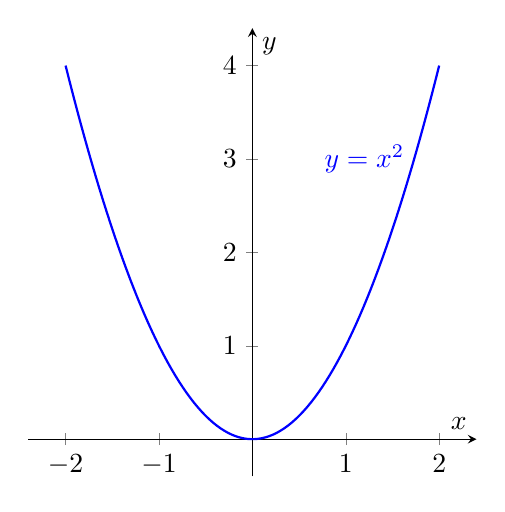
\begin{tikzpicture}
  \begin{axis}[
      axis lines = center,
      xlabel = {$x$},
      ylabel = {$y$},
      samples=100,
      scale=1,
      axis equal image,
      enlargelimits=true,
    ]
    
    \addplot[blue, thick, domain=-2:2] {x^2};
    \node[blue] at (1.2,3) {$y=x^2$};
  \end{axis}
\end{tikzpicture}
\end{center}

\end{enumerate}

\item \begin{enumerate}[leftmargin=*,label=\textbf{\alph*.}]
\item \begin{enumerate}[leftmargin=*,label=\textbf{\roman*.}]
\item If $\mathbf u$ and $\mathbf v$ are perpendicular, the dot product of these vectors is equal to zero.
\[\mathbf u\cdot\mathbf v=\left\langle6,-3,2\right\rangle\cdot\left\langle4p+1,\,p-2,\,1\right\rangle=6(4p+1)-3(p-2)+2\cdot1=21p+14=0\]
\[\implies \boxed{p=-\frac23}\]

\item If $\mathbf u$ and $\mathbf v$ are parallel, the cross product of these vectors is equal to the zero vector.
\begin{align*}\mathbf{u}\times\mathbf{v}&=\left|\begin{array}{ccc}
\mathbf{i}&\mathbf{j}&\mathbf{k}\\
6&-3&2\\
4p+1&p-2&1
\end{array}\right|\\[1em]&=\mathbf{i}\left|\begin{array}{cc}
-3&2\\p-2&1
\end{array}\right|-\mathbf{j}\left|\begin{array}{cc}
6&2\\4p+1&1
\end{array}\right|+\mathbf{k}\left|\begin{array}{cc}
6&-3\\4p+1&p-2
\end{array}\right|\\[1em]&=[1\cdot(-3)-2(p-2)]\,\mathbf i-(6\cdot1-2(4p+1))\,\mathbf j +\\&\quad +[6(p-2)-(-3)(4p+1)]\,\mathbf k\\[1em]&=(1-2p)\,\mathbf i-(4-8p)\,\mathbf j+(-9+18p)\,\mathbf k=\mathbf0\implies \boxed{p=\frac12}\end{align*}

\end{enumerate}
\item The sides of an equilateral triangle have the same length.
\[\overrightarrow{AB}=\left\langle3-5,\,1-1,\,5-3\right\rangle=\left\langle-2,0,2\right\rangle\rightarrow\left|\overrightarrow{AB}\right|=\sqrt{(-2)^2+0^2+2^2}=\sqrt8\]
\[\overrightarrow{AC}=\left\langle5-5,\,3-1,\,5-3\right\rangle=\left\langle0,2,2\right\rangle\rightarrow\left|\overrightarrow{AC}\right|=\sqrt{0^2+2^2+2^2}=\sqrt8\]
\[\overrightarrow{BC}=\left\langle5-3,\,3-1,\,5-5\right\rangle=\left\langle2,2,0\right\rangle\rightarrow\left|\overrightarrow{AC}\right|=\sqrt{2^2+2^2+0^2}=\sqrt8\]

Half of the magnitude of the cross product of two vectors gives us the area of the triangle.
\[\frac12\left|\overrightarrow{AB}\times\overrightarrow{AC}\right|=\frac12\left|\overrightarrow{AB}\right|\left|\overrightarrow{AC}\right|\sin\frac\pi3=\frac12\cdot\sqrt8\cdot\sqrt8\cdot\frac{\sqrt3}2=\boxed{2\sqrt3}\]

\end{enumerate}

\item \begin{enumerate}[leftmargin=*,label=\textbf{\alph*.}]
\item The planes have the same normal $\mathbf n=\left\langle1,1,1\right\rangle$. Using the definition $\mathbf n\cdot\overrightarrow{PP_0}=0$, we obtain
\[1(x-1)+1(y-2)+1(z-3)=0\implies\boxed{x+y+z=6}\]

\item The direction vector of the line is the normal vector of the plane. Therefore, the parametric equations for the line $L$ is as follows.
\[\boxed{\left.\begin{array}{l}
x=1+t\\
y=2+t\\
z=3+t
\end{array}\right\}\quad t\in\mathbb{R}}\]

\item Substitute the equation of $L$ in the equation of the plane $R$.
\[x+y+z=1\implies (1+t)+(2+t)+(3+t)=1\implies 3t+6=1\implies t=-\frac53\]
\[t=-\frac53\implies x=1-\frac53=-\frac23,\quad y=2-\frac53=\frac13,\quad z=3-\frac53=\frac43\]

Therefore, the point of intersection is $\boxed{\left(-\frac23,\frac13,\frac43\right)}$.
\end{enumerate}

\item \begin{enumerate}[leftmargin=*,label=\textbf{\alph*.}]
\item Apply the Two-Path Test.

\[y=x\implies\lim_{(x,y)\to(0,0)}\frac{x^3y}{x^6+y^2}=\lim_{x\to0}\frac{x^4}{x^6+x^2}=\lim_{x\to0}\frac{x^2}{x^4+1}=\frac01=0\]
\[y=x^3\implies\lim_{(x,y)\to(0,0)}\frac{x^3y}{x^6+y^2}=\lim_{x\to0}\frac{x^6}{2x^6}=\lim_{x\to0}\frac12=\frac12\]

Since $0\neq\dfrac12$, by the Two-Path Test, the limit does not exist.

\item We have the inequality $\left|\sin\theta\right|\leq1$ for all values of $\theta$. Therefore,
\[-1\leq\sin\left(\frac1{x^2+|y|}\right)\leq1\qquad\left[\text{except for }x=0,\,y=0\right]\]
\[-x^4\leq x^4\sin\left(\frac1{x^2+|y|}\right)\leq x^4\]
\[\lim_{(x,y)\to(0,0)}-x^4=\lim_{(x,y)\to(0,0)}x^4=0\implies\lim_{(x,y)\to(0,0)}x^4\sin\left(\frac1{x^2+|y|}\right)=\boxed0\]

By the squeeze theorem, the limit is equal to zero.

\end{enumerate}

\item \begin{enumerate}[leftmargin=*,label=\textbf{\alph*.}]
\item Parametrize the curve using $0\leq t\leq 2\pi$.
\[x=\cos t,\:y=\sin t,\:z=4\cos^2t,\qquad0\leq t\leq2\pi\]
\[\boxed{\mathbf r(t)=\left\langle\cos t,\,\sin t,\,4\cos^2t\right\rangle\qquad0\leq t\leq2\pi}\]

\item The tangent vector can be obtained by taking the first derivative of the vector function.
\[\mathbf T(t)=\mathbf r'(t)=\left\langle-\sin t,\,\cos t,\,-8\cos t\sin t\right\rangle\]

The unit tangent vector is
\[\frac{\mathbf T(t)}{\left|\mathbf T(t)\right|}=\frac{\left\langle-\sin t,\,\cos t,\,-8\cos t\sin t\right\rangle}{\sqrt{(-\sin t)^2+(\cos t)^2+(-8\cos t\sin t)^2}}=\frac{\left\langle-\sin t,\,\cos t,\,-8\cos t\sin t\right\rangle}{\sqrt{1+64\cos^2t\sin^2t}}\]

At $t=\dfrac\pi2$,
\[\frac{\mathbf T(t=\pi/2)}{|\mathbf T(t=\pi/2)|}=\frac{\left\langle-\sin\dfrac\pi2,\,\cos \dfrac\pi2,\,-8\cos\dfrac\pi2\sin\dfrac\pi2\right\rangle}{\sqrt{1+64\cos^2\dfrac\pi2\sin^2\dfrac\pi2}}=\boxed{\left\langle-1,0,0\right\rangle}\]

\item The length of the parametrized curve $\mathbf{r}(t)=\left\langle x(t),\,y(t),\,z(t)\right\rangle$ for $a\leq t\leq b$ can be evaluated using the integral
\[L=\int_a^b\left|\frac{d\mathbf r}{dt}\right|\,dt\]
The length of the curve is then
\begin{align*}L&=\int_0^{2\pi}\left|\frac{d\mathbf r}{dt}\right|\,dt=\boxed{\int_0^{2\pi}\sqrt{1+64\cos^2t\sin^2t}\,dt=\int_0^{2\pi}\sqrt{1+16\sin^22t}\,dt}\end{align*}

\end{enumerate}
\newpage

\item This is a circular paraboloid with the vertex $(0,0,2)$ opening downward along the $z$-axis.

\begin{center}
\begin{tikzpicture}
  \begin{axis}[
  title={Plane $x=0$},
    xlabel=$y$, ylabel=$z$,
    xtick=\empty, ytick=\empty,
    samples=50,
    axis lines=middle,
    clip=true,
    scale=0.9,
    enlargelimits=true
    ]
    \addplot[domain=-5:5, blue] {-x^2/4+2};

    \node[blue] at (2.2,-3) {$z=-y^2+2$};
  \end{axis}
\end{tikzpicture}\hspace{1em}
\begin{tikzpicture}
  \begin{axis}[
  title={Plane $y=0$},
    xlabel=$x$, ylabel=$z$,
    xtick=\empty, ytick=\empty,
    samples=50,
    axis lines=middle,
    clip=true,
    scale=0.9,
    enlargelimits=true
    ]
    \addplot[domain=-5:5, red] {-x^2/4+2};

    \node[red] at (2.2,-3) {$z=-x^2+2$};
  \end{axis}
\end{tikzpicture}

\begin{tikzpicture}
  \begin{axis}[
  title={Plane $z=0$},
  axis equal image,
    xlabel=$x$, ylabel=$y$,
    xtick=\empty, ytick=\empty,
    samples=300,
    axis lines=middle,
    clip=true,
    scale=1,
    enlargelimits=true
    ]
    \addplot[domain=-sqrt(2):sqrt(2), orange] {sqrt(2-x^2)};
    \addplot[domain=-sqrt(2):sqrt(2), orange] {-sqrt(2-x^2)};

    \node[orange] at (0.7,0.2) {$x^2+y^2=2$};
  \end{axis}
\end{tikzpicture}\hspace{1em}
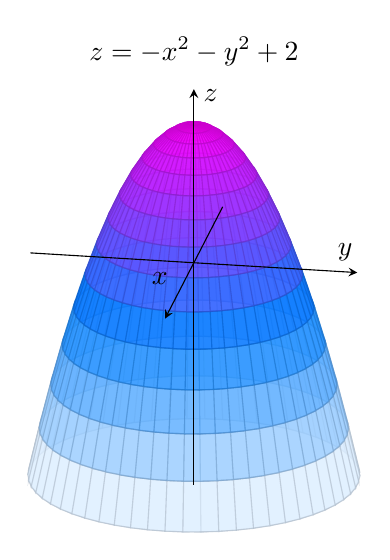
\begin{tikzpicture}
  \begin{axis}[
    title={$\displaystyle z=-x^2-y^2+2$},
    title style={yshift=-25pt},
      view={100}{20},
      axis lines=center,
      axis equal image,
      xlabel={$x$},
      ylabel={$y$},
      zlabel={$z$},
      domain=0:2*pi,
      y domain=-2.25:2.25,
      samples=30,
      samples y=30,
      colormap/cool,
      axis on top,
      scale=1.5,
      xtick=\empty, ytick=\empty, ztick=\empty,
      z buffer=sort,
      zmin=-3.2, zmax=2.5
    ]
    \addplot3[
      surf,
      opacity=0.6
    ]
    ({y*cos(deg(x))},
      {y*sin(deg(x))},
      {-y^2+2});
  \end{axis}
\end{tikzpicture}
\end{center}
\end{enumerate}

\newpage
\stepcounter{subsection}
\phantomsection
\addcontentsline{toc}{subsection}{\protect\numberline{\thesubsection}Midterm - Spring 2026 Solutions}

\fancyhead[R]{\textit{2025-2026 Spring Midterm}}

%Last update: 05/09/2026 01:59

\begin{enumerate}[leftmargin=*,label=\textbf{\arabic*.}]

\item Given cylindrical coordinates $(r, \theta, z) = \left(\sqrt{3}, -\frac{\pi}{4}, -1\right)$. Using conversion formulas:
\begin{align*}
\rho &= \sqrt{r^2 + z^2} = \sqrt{(\sqrt{3})^2 + (-1)^2} = \sqrt{3 + 1} = 2 \\
\theta &= -\frac{\pi}{4} \\
\phi &= \arccos\left(\frac{z}{\rho}\right) = \arccos\left(-\frac{1}{2}\right) = \frac{2\pi}{3}
\end{align*}

Thus $(\rho, \theta, \phi) = \left(2, -\frac{\pi}{4}, \frac{2\pi}{3}\right)$.

$\boxed{\text{Answer: (A)}}$

\item We can solve this question by trial and error. Inspect $r = \cos^2\theta \sin\theta$.
\begin{itemize}[leftmargin=*]
    \item When $\theta = 0, \pi$, $r = 0$.
    \item For $\theta \in (0, \pi)$, $\sin\theta > 0$ and $\cos^2\theta \ge 0$, creating a loop along the positive $y$-axis.
    \item The factor $\cos^2\theta$ pinches the loop at $\theta = \frac{\pi}{2}$, matching the given shape.
\end{itemize}

$\boxed{\text{Answer: (A)}}$

\item Given point $P(1,2,3)$ and plane $x + y + z = 0$ with normal vector $\vec{n} = \langle 1, 1, 1 \rangle$.

The orthogonal line through $P$ is $\vec{r}(t) = \langle 1+t, 2+t, 3+t \rangle$. Substitute into the plane equation.
\[(1+t) + (2+t) + (3+t) = 0 \implies 3t + 6 = 0 \implies t = -2\]

Substitute $t = -2$ back yields the projection point.
\[P' = (1 - 2, 2 - 2, 3 - 2) = (-1, 0, 1)\]

$\boxed{\text{Answer: (A)}}$

\item Find intersection points for $r_1 = 3\cos\theta$ and $r_2 = 1 + \cos\theta$.
\[3\cos\theta = 1 + \cos\theta \implies 2\cos\theta = 1 \implies \theta = \pm \frac{\pi}{3}\]

Calculate area.
\begin{align*}
    A &= \frac{1}{2} \int_{-\pi/3}^{\pi/3} \left( r_1^2 - r_2^2 \right) d\theta = \int_{0}^{\pi/3} \left( 8\cos^2\theta - 2\cos\theta - 1 \right) d\theta \\
      &= \int_{0}^{\pi/3} \left( 3 + 4\cos 2\theta - 2\cos\theta \right) d\theta \\
      &= \left[ 3\theta + 2\sin 2\theta - 2\sin\theta \right]_0^{\pi/3} = \pi
\end{align*}

$\boxed{\text{Answer: (A)}}$

\item Rearrange $2z^2 - \frac{x^2}{2} - y^2 - 5 = 0$.
\[\frac{z^2}{5/2} - \frac{x^2}{10} - \frac{y^2}{5} = 1\]

The standard form $\frac{z^2}{c^2} - \frac{x^2}{a^2} - \frac{y^2}{b^2} = 1$ has two negative minus signs and one positive sign, representing a hyperboloid of two sheets.

$\boxed{\text{Answer: (A)}}$

\item The direction of maximum increase of $f(x,y,z) = x^2 + 2y^2 - 3z$ is given by gradient $\nabla f$:
\[\nabla f = \langle 2x, 4y, -3 \rangle\]

Evaluate at $P(1,1,2)$.
\[\nabla f(1,1,2) = \langle 2, 4, -3 \rangle\]

$\boxed{\text{Answer: (A)}}$

\item Given $w = \ln(x^2 + y^2)$, $x = s\cos t$, and $y = s + \sin t$. At $(s,t) = \left(1, \frac{\pi}{6}\right)$:
\[x = \frac{\sqrt{3}}{2}, \quad y = \frac{3}{2}, \quad x^2 + y^2 = 3\]

Applying the Chain Rule $\frac{\partial w}{\partial t} = \frac{\partial w}{\partial x}\frac{\partial x}{\partial t} + \frac{\partial w}{\partial y}\frac{\partial y}{\partial t}$:
\begin{align*}
    \frac{\partial w}{\partial x} &= \frac{2x}{x^2+y^2} = \frac{\sqrt{3}}{3}, \quad &\frac{\partial x}{\partial t} &= -s\sin t = -\frac{1}{2} \\
    \frac{\partial w}{\partial y} &= \frac{2y}{x^2+y^2} = 1, \quad &\frac{\partial y}{\partial t} &= \cos t = \frac{\sqrt{3}}{2}
\end{align*}
\[\frac{\partial w}{\partial t} = \left(\frac{\sqrt{3}}{3}\right)\left(-\frac{1}{2}\right) + (1)\left(\frac{\sqrt{3}}{2}\right) = \frac{\sqrt{3}}{3}\]

$\boxed{\text{Answer: (E)}}$

\item For $y = \frac{x^2}{2}$ and $z = \frac{x^3}{6}$, derivatives are $\frac{dy}{dx} = x$ and $\frac{dz}{dx} = \frac{x^2}{2}$.
\begin{align*}
    L &= \int_{0}^{2} \sqrt{1 + \left(\frac{dy}{dx}\right)^2 + \left(\frac{dz}{dx}\right)^2} \, dx = \int_{0}^{2} \sqrt{1 + x^2 + \frac{x^4}{4}} \, dx \\
      &= \int_{0}^{2} \left(1 + \frac{x^2}{2}\right) dx = \left[ x + \frac{x^3}{6} \right]_{0}^{2} = \frac{10}{3}
\end{align*}

$\boxed{\text{Answer: (A)}}$

\item For $F(x,y,z) = x^2 + 2y^2 - z = 0$ and $G(x,y,z) = x^2 + (y-1)^2 - 1 = 0$, gradients at $P(1,1,3)$ are:
\[\nabla F(1,1,3)=\langle 2, 4, -1 \rangle, \quad \nabla G(1,1,3) = \langle 2, 0, 0 \rangle\]

Cross product gives the tangent vector.
\[\vec{v} = \nabla F \times \nabla G = \begin{vmatrix} \mathbf{i} & \mathbf{j} & \mathbf{k} \\ 2 & 4 & -1 \\ 2 & 0 & 0 \end{vmatrix} = \langle 0, -2, -8 \rangle\]

Negating yields the parallel vector $\langle 0, 2, 8 \rangle$.

$\boxed{\text{Answer: (A)}}$

\item Intersecting $z = x^2 + y^2$ and $z = 4$ gives $x^2 + y^2 = 4$ in the plane $z = 4$.

Standard parametrization is
\[\vec{r}(t)=\langle2\cos t,2\sin t,4\rangle\]

$\boxed{\text{Answer: (A)}}$

\item Jacobian matrix with respect to $(u,v)$ at $P(1,0,1,1)$:
\[J = \begin{bmatrix} \frac{\partial x}{\partial u} & \frac{\partial x}{\partial v} \\[1em] \frac{\partial y}{\partial u} & \frac{\partial y}{\partial v} \end{bmatrix}_{\text{at } P}  = \begin{bmatrix} 2xuv - y\sin u & xu^2 \\ \frac{1}{u} - 1 & \frac{1}{v} + 1 \end{bmatrix}_{\text{at } P} = \begin{bmatrix} 2 & 1 \\ 0 & 2 \end{bmatrix}\]

Since $\det(J)=2\cdot2-1\cdot0=4\neq0$, the system defines $u, v$ implicitly near $P$. Differentiate with respect to $y$.
\begin{align*}
    2u \frac{\partial u}{\partial y} + \frac{\partial v}{\partial y} + \cos(1) &= 0 \implies 2\frac{\partial u}{\partial y} + \frac{\partial v}{\partial y} = -\cos(1) \\
    2\frac{\partial v}{\partial y} + 1 &= 0 \implies \frac{\partial v}{\partial y} = -\frac{1}{2}
\end{align*}

Substitute $\frac{\partial v}{\partial y}$.

\[\boxed{\frac{\partial u}{\partial y} = \frac{1 - 2\cos(1)}{4}}\]

\item \begin{enumerate}[label=\textbf{\alph*.}]
    \item Use the formal definition of $f_x(0,0)$.
    \[f_x(0,0) = \lim_{h \to 0} \frac{f(h,0) - f(0,0)}{h} = \lim_{h \to 0} \frac{\frac{h^2 + \sin(h)}{h} - 1}{h} = \lim_{h \to 0} \frac{h^2 + \sin(h) - h}{h^2}\]
    Use L'Hôpital's rule twice.
    \[f_x(0,0) \overset{\text{L'H.}}= \lim_{h\to0}\frac{2h+\cos h-1}{2h}\overset{\text{L'H.}}= \lim_{h\to0}\frac{2-\sin h}{2}=\frac{2-0}2=\boxed1\]
    \item Approach $\displaystyle\lim_{(x,y)\to(0,0)} \frac{x^3 y^2}{x^6 + y^4}$ along paths $y = k x^{3/2}$.
    \[\lim_{x \to 0^+} \frac{x^3 (k^2 x^3)}{x^6 + k^4 x^6} = \frac{k^2}{1 + k^4}\]
    Since the result depends on $k$, $\boxed{\text{the limit does not exist}}$.
\end{enumerate}

\item The extreme value theorem states that a continuous function on a specific region will always have its absolute maxima and minima. $f$ is continuous everywhere on its domain. Check the interior points.
\[\nabla f = \langle 2x - 2, 2y + 4 \rangle = \langle 0, 0 \rangle \implies (1, -2)\]

Check if the point is inside the region.
\[y > x -4\longrightarrow 1 - (-2) = 3 < 4\]

$(1,-2)$ is inside. We have $f(1,-2) = -5$.

Check the boundary.
\begin{itemize}[leftmargin=*]
    \item $x=0$: $g(y) = y^2 + 4y \implies y = -2 \implies f(0,-2) = -4$
    \item $y=0$: $h(x) = x^2 - 2x \implies x = 1 \implies f(1,0) = -1$
    \item $y = x - 4$: $k(x) = 2x^2 - 6x \implies x = \frac{3}{2},\: y = -\frac{5}{2} \implies f\left(\frac{3}{2}, -\frac{5}{2}\right) = -4.5$
\end{itemize}

Check the endpoints. At endpoints: $f(0,0) = 0$, $f(0,-4) = 0$, and $f(4,0) = 8$.

Compare all the values obtained.

\[\boxed{\text{Absolute minimum value is }{-5}\text{ at }(1,-2).\text{ Absolute maximum value is }8\text{ at }(4,0).}\]

\end{enumerate}

\newpage
\renewcommand{\headrulewidth}{0pt}
\fancyhead[L]{}
\fancyhead[R]{}

\stepcounter{section}
\vspace*{\fill}
\begin{center}
\phantomsection
\addcontentsline{toc}{section}{\protect\numberline{\thesection}Final Solutions}
\Huge \textbf{FINAL SOLUTIONS}
\end{center}
\vspace*{\fill}

\newpage
\renewcommand{\headrulewidth}{1pt}
\fancyhead[L]{\textit{Hacettepe MAT124 Exam Solutions Version 2}}

\stepcounter{subsection}
\phantomsection
\addcontentsline{toc}{subsection}{\protect\numberline{\thesubsection}Final - Spring 2020 Solutions}

\fancyhead[R]{\textit{2019-2020 Spring Final}}

%(Last update: 19/8/25 (19th of August) 22:37)

\begin{enumerate}[leftmargin=*,label=\textbf{\arabic*.}]
\item Let $g(x,y,z)=x^2+y^2+z^2-100$ and then, solve the system of equations below using the method of Lagrange multipliers.

\[
\left.
\begin{array}{l}
\displaystyle\nabla f=\lambda\nabla g\\
\displaystyle g(x,y,z)=0
\end{array}
\right\}\quad\begin{array}{c}
\nabla f=\left\langle1,-1,1\right\rangle=\lambda\left\langle2x,2y,2z\right\rangle=\lambda\nabla g\\[1em]\displaystyle\therefore\: x=\frac1{2\lambda},\quad y=-\frac1{2\lambda},\quad z=\frac1{2\lambda}
\end{array}
\]

Use the constraint.
\[g(x,y,z)=0\implies\left(\frac1{2\lambda}\right)^2+\left(-\frac1{2\lambda}\right)^2+\left(\frac1{2\lambda}\right)^2=100\implies\frac3{4\lambda^2}=100\]

\[\implies\lambda=\pm\frac{\sqrt3}{20\lambda}\implies x=\pm\frac{10\sqrt3}3,\quad y=\mp\frac{10\sqrt3}3,\quad z=\pm\frac{10\sqrt3}3\quad\]

The absolute extrema occur at $\left(\frac{10\sqrt3}3,-\frac{10\sqrt3}3,\frac{10\sqrt3}3\right)$ and $\left(-\frac{10\sqrt3}3,\frac{10\sqrt3}3,-\frac{10\sqrt3}3\right)$.
\[f\left(\frac{10\sqrt3}3,-\frac{10\sqrt3}3,\frac{10\sqrt3}3\right)=10\sqrt3,\quad f\left(-\frac{10\sqrt3}3,\frac{10\sqrt3}3,-\frac{10\sqrt3}3\right)=-10\sqrt3\]

\[\boxed{\text{The minimum value is }{-10\sqrt3}\text{ and the maximum value is }10\sqrt3.}\]

\item Recall that 12 inches is 1 foot. The volume of a right circular cylinder is
\[V(r,h)=\pi r^2 h\]

The total differential is
\[dV=V_r\,dr+V_h\,dh=\pi\left(2r\cdot h\right)\,dr+\pi\left(r^2\cdot 1\right)\,dh\]

Set $r=1,\:h=4,\:dr=-0.2/12=-1/60,\:dh=-0.4/12=-1/30$.
\[dV=\pi\left(2\cdot1\cdot 4\right)\cdot\left(-\frac1{60}\right)+\pi\left(1^2\right)\left(-\frac1{30}\right)=-\frac\pi6\]

Calculate the volume of the outer cylinder.
\[V(1,4)=\pi\cdot1^2\cdot4=4\pi\]

Take $\displaystyle\Delta V\approx dV=-\frac\pi6$. Therefore, the volume of the interior can be approximated as follows.
\[\boxed{V\approx4\pi-\frac\pi6=\frac{23\pi}6}\]

\newpage

\item We have $x=r\cos\theta$ and $y=r\sin\theta$. Compute the first-order partial derivatives.
\[\frac{\partial z}{\partial r}=\frac{\partial z}{\partial x}\cdot\frac{\partial x}{\partial r}+\frac{\partial z}{\partial y}\cdot\frac{\partial y}{\partial r},\qquad\frac{\partial z}{\partial \theta}=\frac{\partial z}{\partial x}\cdot\frac{\partial x}{\partial \theta}+\frac{\partial z}{\partial y}\cdot\frac{\partial y}{\partial \theta}\]
\[\frac{\partial x}{\partial r}=\cos\theta,\qquad\frac{\partial y}{\partial r}=\sin\theta,\qquad\frac{\partial x}{\partial \theta}=-r\sin\theta,\qquad\frac{\partial y}{\partial\theta}=r\cos\theta,\]

Rewrite $\displaystyle\frac{\partial z}{\partial r}$ and $\displaystyle\frac{\partial z}{\partial\theta}$.
\[\frac{\partial z}{\partial r}=\frac{\partial z}{\partial x}\cdot\cos\theta+\frac{\partial z}{\partial y}\cdot\sin\theta\]
\[\frac{\partial z}{\partial\theta}=\frac{\partial z}{\partial x}\cdot(-r\sin\theta)+\frac{\partial z}{\partial y}\cdot(r\cos\theta)\implies\frac1r\cdot\frac{\partial z}{\partial\theta}=\frac{\partial z}{\partial x}\cdot(-\sin\theta)+\frac{\partial z}{\partial y}\cdot\cos\theta\]

Take the squares of both sides of the equations and add up side by side.
\[\left(\frac{\partial z}{\partial r}\right)^2=\left(\frac{\partial z}{\partial x}\cdot\cos\theta+\frac{\partial z}{\partial y}\cdot\sin\theta\right)^2,\quad\left(\frac1r\cdot\frac{\partial z}{\partial\theta}\right)^2=\left(\frac{\partial z}{\partial x}\cdot(-\sin\theta)+\frac{\partial z}{\partial y}\cdot\cos\theta\right)^2\]
\begin{align*}
\left(\frac{\partial z}{\partial r}\right)^2+\frac1{r^2}\left(\frac{\partial z}{\partial\theta}\right)^2&=\left(\frac{\partial z}{\partial x}\right)^2\cos^2\theta+2\cdot\frac{\partial z}{\partial x}\cdot\frac{\partial z}{\partial y}\cdot\cos\theta\sin\theta+\left(\frac{\partial z}{\partial y}\right)^2\sin^2\theta\\[1em]&\quad\:\;+\left(\frac{\partial z}{\partial x}\right)^2\sin^2\theta-2\cdot\frac{\partial z}{\partial x}\cdot\frac{\partial z}{\partial y}\cdot\cos\theta\sin\theta+\left(\frac{\partial z}{\partial y}\right)^2\cos^2\theta
\end{align*}

The terms with $\sin\theta\cos\theta$ cancel each other. Recall the equation $\displaystyle \sin^2x+\cos^2x=1$. The equation then becomes
\[\left(\frac{\partial z}{\partial r}\right)^2+\frac1{r^2}\left(\frac{\partial z}{\partial\theta}\right)^2=\left(\frac{\partial z}{\partial x}\right)^2+\left(\frac{\partial z}{\partial y}\right)^2,\]

which we set out to demonstrate.

\item Sketch the region.

\begin{center}
\begin{minipage}{0.5\textwidth}
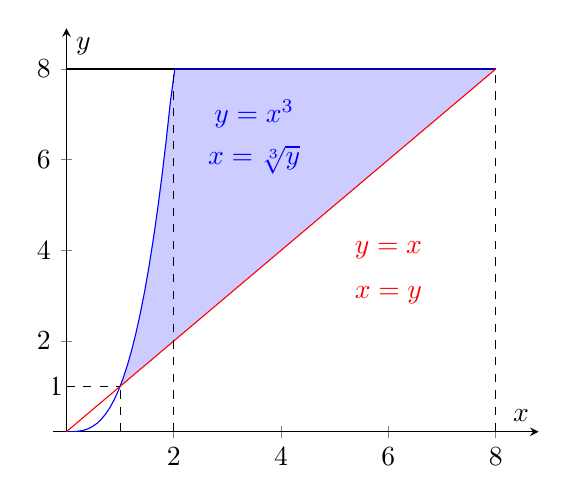
\begin{tikzpicture}
  \begin{axis}[
      axis lines = middle,
      xlabel = $x$, ylabel = $y$,
      domain=0:8,
      ymin=0, ymax=8.9,
      xmin=-0.25, xmax=8.8,
      samples=100,
      clip=true,
      scale=0.9,
    ]
    
    \addplot [name path=A, domain=1:8, draw=none] {x};
    \addplot [name path=B, domain=1:8, draw=none] {min(x^3,8)};
    \addplot [fill=blue!20, draw=none] fill between [of=A and B, soft clip={domain=1:8}];

    \node at (-0.2,1) {$1$};
    \draw[thick] (0,8)--(8,8);
    \addplot [blue, domain=0:8] {min(x^3,8)};
    \addplot [red, domain=0:8] {x};
    \draw[dashed] (1,0)--(1,1); \draw[dashed] (0,1)--(1,1); \draw[dashed] (2,0)--(2,8); \draw[dashed] (8,0)--(8,8);

    \node[red] at (6,4) {$y=x$}; \node[red] at (6,3) {$x=y$};
    \node[blue] at (3.5,7) {$y=x^3$}; \node[blue] at (3.5,6) {$x=\sqrt[3]{y}$};
  \end{axis}
\end{tikzpicture}
\end{minipage}\begin{minipage}{0.45\textwidth}
\[\boxed{\int_1^8\int_{\sqrt[3]y}^yf(x,y)\,dx\,dy}\]
\end{minipage}
\end{center}

\newpage

\item\leavevmode

\vspace{-3em}
\begin{align*}\int_1^2\int_{y^2}^{y^5}{e}^{x/y^2}\,dx\,dy&=\int_1^2\left[y^2\cdot{{e}^{x/y^2}}\right]_{x=y^2}^{x=y^5}\,dy=\int_1^2\left(y^2\cdot{e}^{y^3}-y^2\cdot{e}\right)\,dy\\[1em]&=\left[\frac13{e}^{y^3}-\frac13{e}y^3\right]_1^2=\frac13{e}^{8}-\frac{8{e}}3-\left(\frac13{e}^1-\frac13{e}\right)=\boxed{\frac{{e}}3\left({e}^7-8\right)}\end{align*}

\item\leavevmode

\vspace{-2em}
\begin{center}
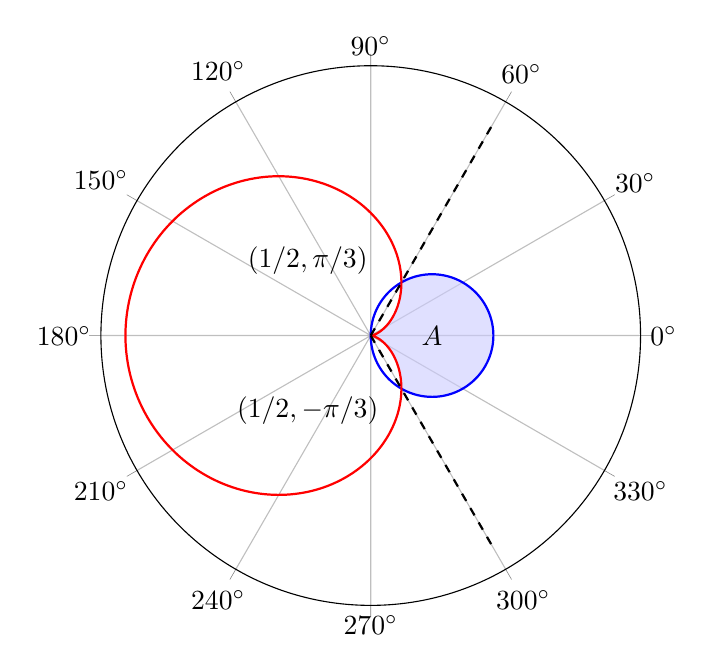
\begin{tikzpicture}
  \begin{polaraxis}[ytick=\empty, axis y line=none, xticklabel=$\pgfmathprintnumber{\tick}^\circ$,]
    \addplot [
      domain=-pi/3:pi/3,
      samples=300,
      draw=none,
      name path=A,
      data cs=polarrad,
    ] {cos(deg(x))};

    \addplot [
      domain=-pi/3:pi/3,
      samples=300,
      draw=none,
      name path=B,
      data cs=polarrad,
    ] {1-cos(deg(x))};

    \addplot [
      blue!20,
      fill opacity=0.6,
    ] fill between[of=A and B];

    \addplot [
      domain=0:2*pi,
      samples=300,
      thick,
      blue,
      data cs=polarrad,
    ] {cos(deg(x))};

    \addplot [
      domain=0:2*pi,
      samples=300,
      thick,
      red,
      data cs=polarrad,
    ] {1-cos(deg(x))};

    \draw[black, thick, dashed] (axis cs: 60,0) -- (axis cs: 60,2);
    \draw[black, thick, dashed] (axis cs: -60,0) -- (axis cs: -60,2);

    \node at (axis cs:130,0.8) {$(1/2,\pi/3)$};
    \node at (axis cs:-130,0.8) {$(1/2,-\pi/3)$};
    \node at (0,0.5) {$A$};

  \end{polaraxis}
\end{tikzpicture}
\end{center}
\begin{align*}
A&=\int_{-\pi/3}^{\pi/3}\int_{1-\cos\theta}^{\cos\theta}\,r\,dr\,d\theta=\frac12\int_{-\pi/3}^{\pi/3}\left[\cos^2\theta-(1-\cos\theta)^2\right]d\theta=\frac12\int_{-\pi/3}^{\pi/3}\left(2\cos\theta-1\right)d\theta\\[1em]&=\frac12\bigg[2\sin\theta-\theta\bigg]_{-\pi/3}^{\pi/3}=\frac12\left[\left(2\sin\frac\pi3-\frac\pi3\right)-\left(2\sin\left(-\frac\pi3\right)+\frac\pi3\right)\right]=\boxed{\sqrt3-\frac\pi3}
\end{align*}

\item For cylindrical coordinates, we have
\[
\left.\begin{array}{c}
z=z\\
r^2=x^2+y^2\\
dV=r\,dz\,dr\,d\theta
\end{array}\right\}\quad\implies\quad
\begin{array}{c}
\displaystyle z=\sqrt{x^2+y^2}\implies z=\sqrt{r^2}\implies z_{\text{lower}}=r\\[1em]
z=2-x^2-y^2\implies z_{\text{upper}}=2-r^2\\[1em]
0\leq\theta\leq2\pi
\end{array}
\]

Find where the surfaces $z=r$ and $z=2-r^2$ intersect to determine the upper bound of $r$.
\begin{align*}\left.\begin{array}{c}
z=r\\
z=2-r^2
\end{array}\right\}\quad r^2+r-2=0\implies (r+2)(r-1)=0\implies r_{\text{upper}}=1\end{align*}

\begin{align*}{I}&=\int_0^{2\pi}\int_0^1\int_{r}^{2-r^2}r\,dz\,dr\,d\theta=\int_0^{2\pi}\int_0^1\bigg[z\bigg]_{z=r}^{z=2-r^2}r\,dr\,d\theta\\[1em]&=\int_0^{2\pi}\int_0^1\left(2-r^2-r\right)\,r\,dr\,d\theta=\int_0^{2\pi}\int_0^1\left(2r-r^3-r^2\right)\,dr\,d\theta\\[1em]&=\int_0^{2\pi}\left[r^2-\frac{r^4}4-\frac{r^3}3\right]_{r=0}^{r=1}\,d\theta=\int_0^{2\pi}\frac5{12}\,d\theta=\frac5{12}\cdot\theta\,\bigg|_0^{2\pi}=\boxed{\frac{5\pi}6}\end{align*}

\item For spherical coordinates, we have
\[
\left.\begin{array}{c}
z=\rho\cos\phi\\
r=\rho\sin\phi\\
x^2+y^2+z^2=\rho^2\\
dV=\rho^2\sin\phi\,d\rho\,d\phi\,d\theta
\end{array}\right.\begin{array}{c}
x^2+y^2+z^2=7\implies\rho^2=7\implies\rho_{\text{upper},1}=\sqrt7\\
z=x^2+y^2\implies\rho\cos\phi=\rho^2\sin^2\phi\implies\rho_{\text{upper},2}=\dfrac{\cos\phi}{\sin^2\phi}\\[1em]
\sin\left(\sqrt{x^2+y^2+z^2}\right)=\sin\left(\sqrt{\rho^2}\right)=\sin\rho\\[1em]
\displaystyle0\leq\theta\leq\frac\pi2
\end{array}\]

Find where the surfaces $z=x^2+y^2$ and $x^2+y^2+z^2=7$ intersect to find the bounds of $\phi$.
\[\begin{array}{c}\displaystyle z^2+z-7=0\implies z_{1,2}=\frac{-1\pm\sqrt{1^2-4\cdot1\cdot(-7)}}2\\[1em]\displaystyle z>0\implies z=\rho\cos\phi=\sqrt7\cos\phi=\frac{-1+\sqrt{29}}{2}\\[1em]\displaystyle\cos\phi=\frac{-1+\sqrt{29}}{2\sqrt7}\implies\phi=\arccos\left(\frac{-1+\sqrt{29}}{2\sqrt7}\right)\end{array}\]

For $\phi<\arccos\left(\frac{-1+\sqrt{29}}{2\sqrt7}\right)$, the upper bound for $\rho$ is $\sqrt7$. For $\phi>\arccos\left(\frac{-1+\sqrt{29}}{2\sqrt7}\right)$, the upper bound is $\dfrac{\cos\phi}{\sin^2\phi}=\cot\phi\csc\phi$.
\[\boxed{\begin{array}{l}\displaystyle\int_0^{\pi/2}\int_0^{\arccos\left(\textstyle\frac{-1+\sqrt{29}}{2\sqrt7}\right)}\int_0^{\sqrt7}\sin\rho \cdot\rho^2\sin\phi\,d\rho\,d\phi\,d\theta\\[1em]\displaystyle+\int_0^{\pi/2}\int_{\arccos\left(\textstyle\frac{-1+\sqrt{29}}{2\sqrt7}\right)}^{\pi/2}\int_0^{\cot\phi\csc\phi}\sin\rho\cdot\rho^2\sin\phi\,d\rho\,d\phi\,d\theta\end{array}}\]

Since we choose the minimum of the upper bounds of $\rho$, we can write the equivalent expression.
\[\boxed{\int_0^{\pi/2}\int_0^{\pi/2}\int_0^{\min\left(\sqrt7,\cot\phi\csc\phi\right)}\sin\rho\cdot\rho^2\sin\phi\,d\rho\,d\phi\,d\theta}\]

\end{enumerate}

\newpage
\pagestyle{fancy}
\renewcommand{\headrulewidth}{1pt}
\fancyhead[R]{\textit{2019-2020 Spring Resit}}
\fancyhead[L]{\textit{Hacettepe MAT124 Exam Solutions Version 2}}

%(Last update: 19/8/25 (19th of August) 22:37)

\begin{enumerate}[leftmargin=*,label=\textbf{\arabic*.}]
\item Let $g(x,y,z)=x+y+z-10$ and then, solve the system of equations below using the method of Lagrange multipliers.
\[
\left.
\begin{array}{ll}
\nabla T =\lambda \nabla g\\[1em]
g(x,y,z) = 0
\end{array}
\right\}\quad
\nabla T = \left\langle-y-z,-x-z,-x-y\right\rangle=\lambda\left\langle1,1,1\right\rangle= \lambda\nabla g
\]

\vspace{-1em}
\begin{align*}T_x+T_y + T_z&=(-y-z) +(-x-z) +(-x-y)=-2x-2y-2z\\[1em]&=\lambda+\lambda+\lambda=3\lambda\implies x+y+z=\frac{-3\lambda}{2}\end{align*}

Use the constraint to find the value of $\lambda$.
\[g(x,y,z) = 0 \implies \frac{-3\lambda}{2}-10=0\implies \lambda=-\frac{20}{3}\]

So far, we have the equations below. Solve the system of equations and find the values of $x,y,z$ one by one.
\begin{align}
-y-z &= -\frac{20}{3}
\label{eq:19_20_spring_resit_1}\\
-x-z &= -\frac{20}{3}
\label{eq:19_20_spring_resit_2}\\
-x-y &= -\frac{20}{3}
\label{eq:19_20_spring_resit_3}
\end{align}

Solve for $x$ and $z$.
\begin{align}
\eqref{eq:19_20_spring_resit_1} \:\&\:
\eqref{eq:19_20_spring_resit_2}
\implies x-y &= 0
\label{eq:19_20_spring_resit_4}\\
\eqref{eq:19_20_spring_resit_3} \:\&\:
\eqref{eq:19_20_spring_resit_4}
\implies y = \frac{10}{3}
\label{eq:19_20_spring_resit_5}\nonumber
\end{align}
\[\therefore\quad z=\frac{10}{3},\qquad x=\frac{10}{3}.\]

We now have all the values. Substitute in $T(x,y,z)$ to find the minimum value of the temperature.
\[T_{\text{min}}=T\left(\frac{10}{3},\frac{10}{3},\frac{10}{3}\right)=100-\left(\frac{10}{3}\right)^2-\left(\frac{10}{3}\right)^2-\left(\frac{10}{3}\right)^2=\boxed{\frac{200}{3}}\]

\item We have $x=r\cos\theta$ and $y=r\sin\theta$.
\[x^2=r^2\cos^2\theta,\quad y^2 =r^2\sin^2\theta\implies x^2+y^2=r^2\left(\cos^2\theta+\sin^2\theta\right)=r^2, \quad r=\sqrt{x^2+y^2}\]
\[\frac{y}{x}=\frac{r\sin\theta}{r\cos\theta}=\tan\theta \implies \theta=\tan^{-1}\frac{y}{x}\]

Compute the first-order partial derivatives.
\[\frac{\partial z}{\partial x}=\frac{\partial z}{\partial r}\cdot\frac{\partial r}{\partial x}+\frac{\partial z}{\partial \theta}\cdot\frac{\partial\theta}{\partial x},\quad\quad\frac{\partial z}{\partial y}=\frac{\partial z}{\partial r}\cdot\frac{\partial r}{\partial y} + \frac{\partial z}{\partial\theta}\cdot\frac{\partial\theta}{\partial y}\]

\vspace{-1em}
\[\frac{\partial r}{\partial x}=\frac{x}{\sqrt{x^2+y^2}}=\cos\theta,\quad\quad\frac{\partial r}{\partial y}=\frac{y}{\sqrt{x^2+y^2}}=\sin\theta\]
\[\quad\frac{\partial\theta}{\partial x}=\frac{1}{1+\frac{y^2}{x^2}}\cdot \left(-\frac{y}{x^2}\right)=\frac{-y}{x^2+y^2}=\frac{-\sin\theta}{r},\quad\quad\frac{\partial\theta}{\partial y}=\frac{1}{\frac{y^2}{x^2}}\cdot\frac{1}{x}=\frac{x}{x^2+y^2}=\frac{\cos\theta}{r}\]

Rewrite $\displaystyle\frac{\partial z}{\partial x}$ and $\displaystyle\frac{\partial z}{\partial y}$.
\[\frac{\partial z}{\partial x}=\frac{\partial z}{\partial r}\cdot\frac{x}{\sqrt{x^2+y^2}}+\frac{\partial z}{\partial\theta}\cdot\frac{-y}{x^2+y^2},\quad\quad\frac{\partial z}{\partial y}=\frac{\partial z}{\partial r}\cdot\frac{y}{\sqrt{x^2+y^2}}+\frac{\partial z}{\partial \theta}\cdot\frac{x}{x^2+y^2}\]

Compute the second-order partial derivatives.
\[\frac{\partial}{\partial x}\left(\frac{\partial z}{\partial x}\right)=\frac{\partial}{\partial x}\left(\frac{\partial z}{\partial r}\cdot\frac{x}{\sqrt{x^2+y^2}}+\frac{\partial z}{\partial\theta}\cdot\frac{-y}{x^2+y^2}\right)\]
\vspace{-1em}
\begin{align*}\frac{\partial^2z}{\partial x^2}=&\left[\left(\frac{\partial^2z}{\partial r^2}\cdot\frac{\partial r}{\partial x}+\frac{\partial^2 z}{\partial\theta\,\partial r}\cdot\frac{\partial\theta}{\partial x}\right)\cdot\frac{x}{\sqrt{x^2+y^2}}+\frac{\partial z}{\partial r}\cdot\frac{1\cdot\sqrt{x^2+y^2}-x\cdot\frac{x}{\sqrt{x^2+y^2}}}{\left(\sqrt{x^2+y^2}\right)^2}\right]\\[1em]&+\left[\left(\frac{\partial^2z}{\partial \theta^2}\cdot\frac{\partial \theta}{\partial x}+\frac{\partial^2 z}{\partial r\,\partial \theta}\cdot\frac{\partial r}{\partial x}\right)\cdot\frac{-y}{x^2+y^2}+\frac{\partial z}{\partial\theta}\cdot\frac{y}{(x^2+y^2)^2}\cdot2x\right]\end{align*}

\[\frac{\partial}{\partial y}\left(\frac{\partial z}{\partial y}\right)=\frac{\partial}{\partial y}\left(\frac{\partial z}{\partial r}\cdot\frac{y}{\sqrt{x^2+y^2}}+\frac{\partial z}{\partial \theta}\cdot\frac{x}{x^2+y^2}\right)\]
\vspace{-1em}
\begin{align*}\frac{\partial^2z}{\partial y^2}=&\left[\left(\frac{\partial^2z}{\partial r^2}\cdot\frac{\partial r}{\partial y}+\frac{\partial^2 z}{\partial\theta\,\partial r}\cdot\frac{\partial\theta}{\partial y}\right)\cdot\frac{y}{\sqrt{x^2+y^2}}+\frac{\partial z}{\partial r}\cdot\frac{1\cdot\sqrt{x^2+y^2}-y\cdot\frac{y}{\sqrt{x^2+y^2}}}{\left(\sqrt{x^2+y^2}\right)^2}\right]\\[1em]&+\left[\left(\frac{\partial^2z}{\partial \theta^2}\cdot\frac{\partial \theta}{\partial y}+\frac{\partial^2 z}{\partial r\,\partial \theta}\cdot\frac{\partial r}{\partial y}\right)\cdot\frac{x}{x^2+y^2}+\frac{\partial z}{\partial\theta}\cdot\frac{-x}{(x^2+y^2)^2}\cdot2y\right]\end{align*}

Add the second-order partial derivatives and set to $0$. The last terms eliminate each other. Write $x$ and $y$ in terms of $r$ and $\theta$.
\begin{align*}\frac{\partial^2 z}{\partial x^2}+\frac{\partial^2 z}{\partial y^2}=&\left[\left(\frac{\partial^2z}{\partial r^2}\cdot\cos\theta +\frac{\partial^2z}{\partial\theta\,\partial r}\cdot\frac{-\sin\theta}{r}\right)\cdot\cos\theta+\frac{\partial z}{\partial r}\cdot\frac{\sin^2\theta}{r}\right]\\[1em]&+\left[\left(\frac{\partial^2z}{\partial\theta^2}\cdot\frac{-\sin\theta}{r} + \frac{\partial^2z}{\partial r\,\partial\theta}\cdot\cos\theta\right)\cdot\frac{-\sin\theta}{r}\right]\\[1em]&+\left[\left(\frac{\partial^2z}{\partial r^2}\cdot\sin\theta +\frac{\partial^2z}{\partial\theta\,\partial r}\cdot\frac{\cos\theta}{r}\right)\cdot\sin\theta+\frac{\partial z}{\partial r}\cdot\frac{\cos^2\theta}{r}\right]\\[1em]&+\left[\left(\frac{\partial^2z}{\partial\theta^2}\cdot\frac{\cos\theta}{r} + \frac{\partial^2z}{\partial r\,\partial\theta}\cdot\sin\theta\right)\cdot\frac{\cos\theta}{r}\right]=0\end{align*}

Inspect the terms that add up to $0$. Recall the identity $\sin^2\theta+\cos^2\theta=1$, then the equation reduces to
\begin{align*}
\frac{\partial^2z}{\partial x^2}+\frac{\partial^2z}{\partial y^2}&=\frac{\partial^2z}{\partial r^2}\cdot\left(\cos^2\theta+\sin^2\theta\right)+\frac{\partial z}{\partial r}\cdot\frac{\sin^2\theta+\cos^2\theta}{r}+\frac1{r^2}\frac{\partial^2z}{\partial\theta^2}\cdot\left(\sin^2\theta+\cos^2\theta\right)\\[1em]&=\boxed{\frac{\partial^2z}{\partial r^2}+\frac1r\frac{\partial z}{\partial r}+\frac1{r^2}\frac{\partial^2z}{\partial\theta^2}=0},
\end{align*}

which we set out to demonstrate.
\item Change the order of integration using the graph below and then evaluate the integral.

\begin{center}
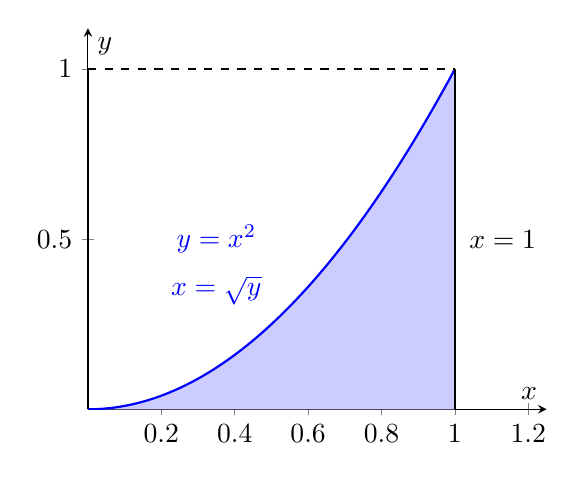
\begin{tikzpicture}
  \begin{axis}[
      axis lines = middle,
      xlabel = $x$, ylabel = $y$,
      domain=0:1,
      ymin=0, ymax=1.12,
      xmin=0, xmax=1.25,
      samples=100,
      clip=true,
      scale=0.85
    ]
    
    \addplot [
      name path=A,
      domain=0:1,
      draw=none,
    ] {x^2};

    \path[name path=B] (axis cs:0,1) -- (axis cs:1,1);
    \path[name path=C] (axis cs:0,0) -- (axis cs:0,1);
    \path[name path=D] (axis cs:0,0) -- (axis cs:1,0);

    \addplot [
      fill=blue!20,
      draw=none,
    ] fill between [
      of=A and D,
      soft clip={domain=0:1},
    ];
    
    \addplot[blue, thick] {x^2};
    \addplot[black, thick] coordinates {(0,0) (0,1)};
    \addplot[black, thick] coordinates {(1,0) (1,1)};
    \draw[dashed] (axis cs: 0,1) -- (axis cs: 1,1);
    \node at (axis cs: 1.13, 0.5) {$x=1$};
    \node[blue] at (axis cs: 0.35, 0.5) {$y=x^2$};
    \node[blue] at (axis cs: 0.35, 0.35) {$x=\sqrt{y}$};

  \end{axis}
\end{tikzpicture}
\end{center}
\begin{align*}
\int_0^1\int_{\sqrt{y}}^1\sqrt{1-x^3}\,dx\,dy&=\int_0^1\int_0^{x^2}\sqrt{1-x^3}\,dy\,dx=\int_0^1x^2\sqrt{1-x^3}\,dx\:\left[{\begin{array}{c}\scriptstyle u=1-x^3 \\\scriptstyle du=-3x^2\,dx\end{array}}\right]\\[1em]&=\int\frac{\sqrt{u}}{-3}\,du=-\frac29u^{3/2}+c=-\frac29\left(1-x^3\right)^{3/2}\Bigg|_0^1=\boxed{\frac29}\end{align*}

\newpage
\item\leavevmode

\vspace{-2em}
\begin{minipage}{0.45\textwidth}
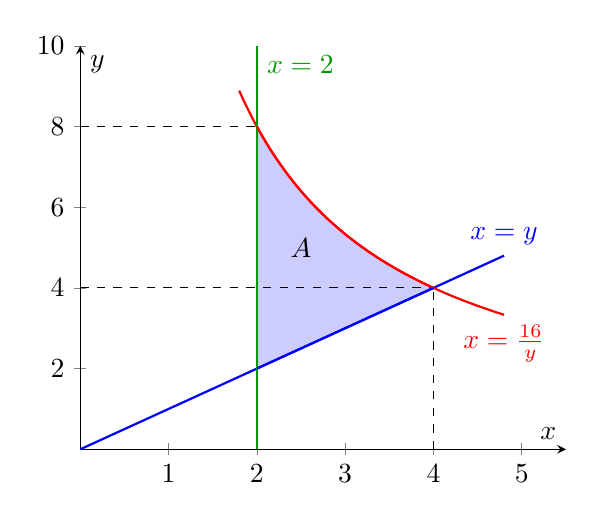
\begin{tikzpicture}
  \begin{axis}[
      axis lines = center,
      xlabel = {$x$},
      ylabel = {$y$},
      domain=1:4,
      samples=200,
      ymin=0, ymax=10,
      xmin=0, xmax=5.5,
      clip=true,
      scale=0.9
    ]
    
    \draw[dashed] (axis cs: 0,4) -- (axis cs: 4,4);
    \draw[dashed] (axis cs: 4,0) -- (axis cs: 4,4);
    \draw[dashed] (axis cs: 0,8) -- (axis cs:2,8);
    \node at (2.5,5) {$A$};

    \addplot[blue, thick, domain=0:4.8] {x} node[above] {$x = y$};

    \addplot[red, thick, domain=1.8:4.8] {16/x} node[below] {$x = \frac{16}{y}$};

    \addplot[green!60!black, thick, domain=0:10] ({2},x) node[below right] {$x = 2$};
    
    \addplot[red, thick, domain=2:4, name path=A] {16/x};
    \addplot[blue, thick, domain=2:4, name path=B] {x};

    \addplot [
      fill=blue!20,
      draw=none,
    ] fill between [
      of=A and B,
      soft clip={domain=2:4},
    ];
  \end{axis}
\end{tikzpicture}
\end{minipage}\hspace{0.25em}
\begin{minipage}{0.46\textwidth}
\begin{align*}A&=\int_2^4\int_2^y\,dx\,dy + \int_4^8\int_2^{16/y}\,dx\,dy\\[1em]&=\int_2^4\int_{x}^{\frac{16}x}\,dy\,dx=\int_2^4\left(\frac{16}x-x\right)\,dx\\[1em]&=\left[16\ln|x| -\frac{x^2}2\right]_2^4\\[1em]&=\left[\left(16\ln4 -\frac{4^2}{2}\right)-\left(16\ln2-\frac{2^2}{2}\right)\right]\\[1em]&=\boxed{16\ln2-6}\end{align*}
\end{minipage}

\item\leavevmode

\vspace{-1em}
\noindent
\begin{minipage}{0.52\linewidth}
    \centering
    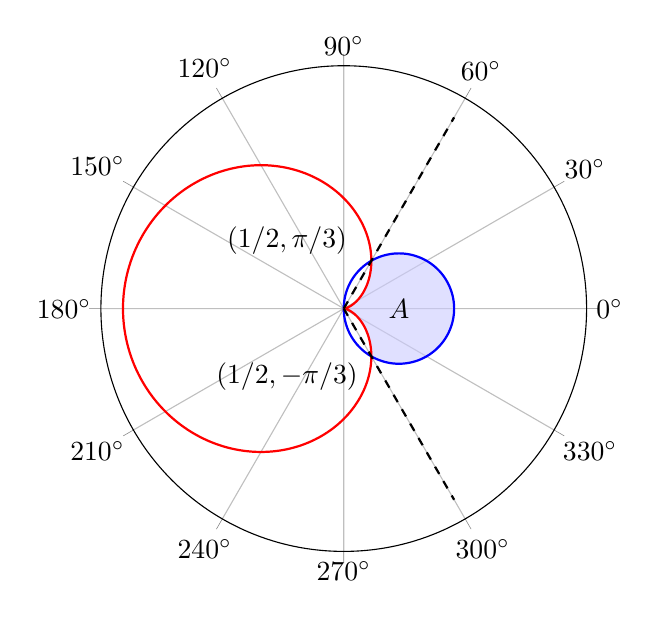
\begin{tikzpicture}
      \begin{polaraxis}[
        ytick=\empty,
        axis y line=none,
        xticklabel=$\pgfmathprintnumber{\tick}^\circ$,
        scale=0.9
      ]
        \addplot [
          domain=-pi/3:pi/3,
          samples=300,
          draw=none,
          name path=A,
          data cs=polarrad,
        ] {cos(deg(x))};

        \addplot [
          domain=-pi/3:pi/3,
          samples=300,
          draw=none,
          name path=B,
          data cs=polarrad,
        ] {1-cos(deg(x))};

        \addplot [
          blue!20,
          fill opacity=0.6,
        ] fill between[of=A and B];

        \addplot [
          domain=0:2*pi,
          samples=300,
          thick,
          blue,
          data cs=polarrad,
        ] {cos(deg(x))};

        \addplot [
          domain=0:2*pi,
          samples=300,
          thick,
          red,
          data cs=polarrad,
        ] {1-cos(deg(x))};

        \draw[black, thick, dashed]
          (axis cs: 60,0) -- (axis cs: 60,2);
        \draw[black, thick, dashed]
          (axis cs: -60,0) -- (axis cs: -60,2);

        \node at (axis cs:130,0.8) {$(1/2,\pi/3)$};
        \node at (axis cs:-130,0.8) {$(1/2,-\pi/3)$};
        \node at (0,0.5) {$A$};

      \end{polaraxis}
    \end{tikzpicture}
\end{minipage}%
\hfill
\begin{minipage}{0.48\linewidth}
    \begin{align*}
    A
    &=\int_{-\pi/3}^{\pi/3}
      \int_{1-\cos\theta}^{\cos\theta}
      r\,dr\,d\theta\\[1em]
    &=\frac12\int_{-\pi/3}^{\pi/3}
      \left[\cos^2\theta-(1-\cos\theta)^2\right]\,d\theta\\[1em]
      &=\frac12\int_{-\pi/3}^{\pi/3}
  \left(2\cos\theta-1\right)\,d\theta\\[1em]
  &=\frac12\bigg[2\sin\theta-\theta\bigg]_{-\pi/3}^{\pi/3}\cdots
    \end{align*}
\end{minipage}

\vspace{1em}
\[\cdots\quad A=\frac12\left[\left(2\sin\frac\pi3-\frac\pi3\right)-\left(2\sin\left(-\frac\pi3\right)+\frac\pi3\right)\right]=\boxed{\sqrt3-\frac\pi3}\]

\item\leavevmode

\vspace{-2em}
\begin{center}
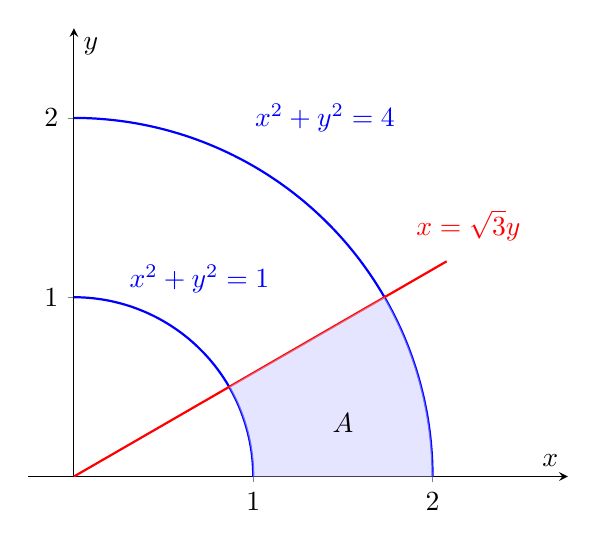
\begin{tikzpicture}
    \begin{axis}[
        axis equal,
        axis lines = center,
        xlabel = $x$,
        ylabel = $y$,
        xmin = 0, xmax = 2.5,
        ymin = 0, ymax = 2.5,
        xtick = {-2,-1,1,2},
        ytick = {-2,-1,1,2},
    ]

    \addplot[domain=0:90, samples=100, blue, thick] ({cos(x)}, {sin(x)});
    \addplot[domain=0:90, samples=100, blue, thick] ({2*cos(x)}, {2*sin(x)});
    \addplot[domain=0:1.2, red, thick] ({sqrt(3)*x}, {x});
    \fill[blue!20, opacity=0.5] 
        plot[domain=0:30, samples=30,variable=\t] ({2*cos(\t)}, {2*sin(\t)}) -- 
        plot[domain=30:0, samples=30,variable=\t] ({cos(\t)}, {sin(\t)}) -- cycle;
    \node[blue] at (1.4,2) {$x^2 + y^2 = 4$};
    \node[blue] at (0.7,1.1) {$x^2 + y^2 = 1$};
    \node[red] at (2.2,1.4) {$x = \sqrt{3}y$};
    \node at (1.5,0.3) {$A$};

    \end{axis}
\end{tikzpicture}
\end{center}

Use the following transformation to switch to polar coordinates.
\[
\left.\begin{array}{c}x=r\cos\theta\\[1em]y=r\sin\theta\\[1em]x^2+y^2=r^2\\[1em]\displaystyle\theta=\tan^{-1}\frac yx\\[1em]dA=r\,dr\,d\theta
\end{array}\right\}\quad\implies\quad
\begin{array}{c}
x^2+y^2=1\,\implies\,r^2=1\implies r=1\\[1em]x^2+y^2=4\,\implies\,r^2=4\implies r=2\\[1em]y=0\implies\theta=0\\[1em]
\displaystyle x=\sqrt3y\implies\tan^{-1}\frac yx=\tan^{-1}\frac1{\sqrt3}\implies\theta=\frac{\pi}6\\[1em]\displaystyle\therefore 1\leq r\leq2,\quad 0\leq\theta\leq\frac{\pi}6
\end{array}
\]
\begin{align*}
\int_0^{\pi/6}\int_1^2\sin(r^2)\,r\,dr\,d\theta&=\int_0^{\pi/6}\left[-\frac12\cos{r^2}\right]_1^2\,d\theta=-\frac12\int_0^{\pi/6}\left(\cos4-\cos1\right)\,d\theta\\[1em]&=\frac12(\cos1-\cos4)\cdot\theta\,\bigg|_0^{\pi/6}=\boxed{\frac\pi{12}(\cos1-\cos4)}
\end{align*}

\item For cylindrical coordinates, we have
\[
\left.\begin{array}{c}
z=z\\[1em]
r^2=x^2+y^2\\[1em]
dV=r\,dz\,dr\,d\theta
\end{array}\right\}\quad\implies\quad
\begin{array}{c}
\displaystyle2z=x^2+y^2\,\implies\,z=\frac{r^2}2\\[1em]
x^2+y^2+z^2=8\,\implies\,z=\sqrt{8-r^2}\\[1em]
\end{array}
\]

Find where the surfaces $2z=x^2+y^2$ and $x^2+y^2+z^2=8$ intersect to determine the limits of $r$.
\begin{align*}x^2+y^2+z^2=8&\implies 2z + z^2 = 8\implies (z+4)(z-2) = 0\implies z=2\\&\implies4=x^2+y^2=r^2 \implies r=2\end{align*}

The lower limit of $r$ is apparently $0$. The region in the $xy$-plane is circular if we project the domain. Therefore, $0\leq\theta\leq2\pi$. Now, set up the triple integral in polar coordinates.
\begin{align*}I&=\iiint_D\frac{dV}{x^2+y^2+z^2}=\int_0^{2\pi}\int_0^2\int_{r^2/2}^{\sqrt{8-r^2}}\frac{r}{r^2+z^2}\,dz\,dr\,d\theta\\[1em]&=\int_0^{2\pi}\int_0^2\int_{r^2/2}^{\sqrt{8-r^2}}\frac{1}{1+\left(\frac zr\right)^2}\cdot\frac1r\,dz\,dr\,d\theta=\int_0^{2\pi}\int_0^2\left[\arctan\left(\frac zr\right)\right]_{r^2/2}^{z=\sqrt{8-r^2}}\,dr\,d\theta\\[1em]&=\int_0^{2\pi}\int_0^2\arctan\left(\frac{\sqrt{8-r^2}}r\right)\,dr\,d\theta-\int_0^{2\pi}\int_0^2\arctan\left(\frac r2\right)\,dr\,d\theta\end{align*}

$\theta$ is independent of $r$. Therefore, we can write the following.
\begin{equation}
I=2\pi\int_0^2\arctan\left(\frac{\sqrt{8-r^2}}r\right)\,dr-2\pi\int_0^2\arctan\left(\frac r2\right)\,dr
\label{eq:19_20_resit_1}
\end{equation}

Now, use integration by parts for the left-hand integral in \eqref{eq:19_20_resit_1}. Apply the chain rule and the quotient rule rigorously.
\begin{align*}
\displaystyle u=\arctan\left(\frac{\sqrt{8-r^2}}r\right)&\implies\displaystyle du=\frac1{1+\left(\frac{\sqrt{8-r^2}}r\right)^2}\cdot\frac{\frac{1}{2\sqrt{8-r^2}}\cdot(-2r)\cdot r -\sqrt{8-r^2}\cdot 1}{r^2}\,dr\\
\displaystyle dv=dr&\implies v=r
\end{align*}

Notice that we have an improper integral, where we need to use limits.
\begin{align}
\int_0^2\arctan\left(\frac{\sqrt{8-r^2}}r\right)\,dr&=\lim_{T\to0^+}\left[r\cdot\arctan\left(\frac{\sqrt{8-r^2}}r\right)\Bigg|_T^2-\int_T^2r\cdot\frac{-1}{\sqrt{8-r^2}}\,dr\right]\nonumber\\[1em]&=\lim_{T\to0^+}\left[r\cdot\arctan\left(\frac{\sqrt{8-r^2}}r\right)-\sqrt{8-r^2}\right]_T^2
\label{eq:19_20_resit_2}
\end{align}

Compute the other integral in \eqref{eq:19_20_resit_1} using integration by parts.
\begin{align*}
\displaystyle u=\arctan\left(\frac{r}2\right)&\implies\displaystyle du=\frac1{\displaystyle1+\left(\frac{r}2\right)^2}\cdot\frac12\,dr\\
\displaystyle dv=dr&\implies v=r
\end{align*}

\vspace{-3em}
\begin{align}
\int_0^2\arctan\left(\frac r2\right)dr&=r\arctan\left(\frac r2\right)\Bigg|_0^2-\int_0^2\frac{2r}{4+r^2}\,dr=\left.r\arctan\frac r 2-\ln\left|4+r^2\right|\right|_0^2
\label{eq:19_20_resit_3}
\end{align}

Rewrite \eqref{eq:19_20_resit_1} using \eqref{eq:19_20_resit_2} and \eqref{eq:19_20_resit_3}.
\begin{align}
I&=2\pi\lim_{T\to0^+}\left[r\cdot\arctan\left(\frac{\sqrt{8-r^2}}r\right)-\sqrt{8-r^2}\right]_T^2-2\pi\left[r\cdot\arctan\left(\frac r2\right)-\ln\left|4+r^2\right|\right]_0^2\nonumber\\[1em]
&=2\pi\left(2\cdot\arctan1-2\right)-2\pi\lim_{T\to0^+}\left[T\cdot\arctan\frac{\sqrt{8-T^2}}T-\sqrt{8-T^2}\right]\nonumber\\[1em]&\quad\:-2\pi\left[\left(2\cdot\arctan1-\ln8\right)-(0-\ln4)\right]\nonumber\\[1em]
&=\pi\left(\ln4-4+2\lim_{T\to0^+}\left(\sqrt{8-T^2}\right)\right)-2\pi\lim_{T\to0^+}\left(T\cdot\arctan\frac{\sqrt{8-T^2}}T\right)
\label{eq:19_20_resit_4}
\end{align}

We need to evaluate the limit on the right side in \eqref{eq:19_20_resit_4} using the squeeze theorem.
\[-\frac\pi2\leq\arctan\left(\frac{\sqrt{8-T^2}}T\right)\leq\frac\pi2\]
\[-\frac{T\cdot\pi}2\leq T\cdot\arctan\left(\frac{\sqrt{8-T^2}}T\right)\leq\frac{T\cdot\pi}2\]
\[\lim_{T\to0^+}\frac{-T\cdot\pi}2=\lim_{T\to0^+}\frac{T\cdot\pi}2=0\implies\lim_{T\to0^+}\left(T\cdot\arctan\frac{\sqrt{8-T^2}}T\right)=0\]

The limit on the left side in \eqref{eq:19_20_resit_4} is simply equal to $2\sqrt2$. The value of the integral is then
\[\boxed{I=\pi\left(\ln4-4+4\sqrt2\right)}\]

\item For spherical coordinates, we have
\[
\left.\begin{array}{c}
z=\rho\cos\phi\\[1em]
r=\rho\sin\phi\\[1em]
x^2+y^2+z^2=\rho^2\\[1em]
dV=\rho^2\sin\phi\,d\rho\,d\phi\,d\theta
\end{array}\right\}\quad\implies\quad
\begin{array}{c}
x^2+y^2+z^2\leq1\,\implies\,\rho^2\leq1\,\implies\,0\leq\rho\leq1\\[1em]
\sqrt{x^2+y^2+z^2}=1\,\implies\,\sqrt{\rho^2}=1\implies\rho=1\\[1em]
\displaystyle\therefore0\leq\theta\leq\frac\pi2,\quad0\leq\phi\leq\frac\pi2
\end{array}
\]

Set up the integral and then evaluate.
\begin{align*}
I&=\iiint_D\sqrt{x^2+y^2+z^2}\,dV=\int_0^{\pi/2}\int_0^{\pi/2}\int_0^1\rho\cdot\rho^2\sin\phi\,d\rho\,d\phi\,d\theta\\[1em]&=\int_0^{\pi/2}\int_0^{\pi/2}\left[\frac{\rho^4}4\right]_{\rho=0}^{\rho=1}\sin\phi\,d\phi\,d\theta=\frac14\int_0^{\pi/2}\int_0^{\pi/2}\sin\phi\,d\phi\,d\theta\\[1em]&=\frac14\int_0^{\pi/2}\bigg[-\cos\phi\bigg]_0^{\pi/2}\,d\theta=\frac14\int_0^{\pi/2}\,d\theta=\boxed{\frac\pi8}
\end{align*}

\end{enumerate}

\newpage
\stepcounter{subsection}
\phantomsection
\addcontentsline{toc}{subsection}{\protect\numberline{\thesubsection}Final - Summer 2020 Solutions}

\fancyhead[R]{\textit{2019-2020 Summer Final}}

%Last update 30/08/2025 02:21

\begin{enumerate}[leftmargin=*,label=\textbf{\arabic*.}]

\item Determine the critical points by setting $f_x=f_y=0$.
\[f_x=2x,\quad f_y=2y-3\]
\[f_x=f_y=0\implies x=0,\quad y=\frac32\]

The \textit{only} critical point occurs at $(0,3/2)$. The value of the function at this point is $f(0, 3/2) = 0^2 + (3/2)^2 -3(3/2)=-9/4$.

Using Lagrange multipliers, find the corresponding points on the boundary. Let $g(x,y)=x^2+y^2-4$ be the constraint. Solve the system of equations below.
\[
\left.
\begin{array}{ll}
\displaystyle\nabla f =\lambda \nabla g\\
\displaystyle g(x,y) = 0
\end{array}
\right\}\quad
\nabla f = \left\langle2x,2y-3\right\rangle=\lambda\left\langle2x,2y\right\rangle= \lambda\nabla g
\]
\[2x(1-\lambda)=0\implies x=0\quad\text{or}\quad\lambda=1\]
\[2y(1-\lambda)-3=0\implies1-\lambda=\frac3{2y}\implies\lambda=1-\frac3{2y}\]
\[x=0\implies g(0,y)=0^2+y^2-4=0\implies y=\pm2\]
\[\lambda=1\implies 2y-3=2y\implies 0\neq-3\quad\therefore\lambda\neq-1\]

Evaluate $f$ at the points $(0,2)$ and $(0,-2)$.
\[f(0,2)=0^2+2^2-3\cdot2=-2,\quad f(0,-2)=0^2+(-2)^2-3\cdot(-2)=10\]

Compare the values $f(0,3/2),\:f(0,2),\:f(0,-2)$.
\[\boxed{f_{\text{max}}=f(0,-2)=10,\quad f_{\text{min}}=f(0,3/2)=-9/4}\]

\item The velocity of a particle can be obtained by taking the first derivative of the position vector of the particle. Since we have the velocity of the particle, we can take the antiderivative. The velocity vector is defined for $t>0$. It is continuous and integrable for $t>0$.
\[\mathbf{V}(t)=\ln t\,\mathbf{i}+\sin t\,\mathbf{j}+t^3\,\mathbf{k}\]
\[\int\mathbf{V}(t)\,dt=\left(\int\ln t\,dt\right)\,\mathbf{i}+\left(\int\sin t\,dt\right)\,\mathbf{j}+\left(\int t^3\,dt\right)\,\mathbf{k}\]

The first integral on the right side can be evaluated with integration by parts. The second integral is related to the integration of trigonometric functions. The last integral is just ordinary integration. The position vector is as follows.
\[\mathbf{R}(t)=(t\ln t- t+c_1)\,\mathbf{i}+(-\cos t+c_2)\,\mathbf{j}+\left(\frac{t^4}4+c_3\right)\,\mathbf{k}\]

\newpage

Evaluate $\mathbf{R}(1)$ to find the constants.
\[\mathbf{R}(1)=(-1+c_1)\,\mathbf{i}+(-\cos1+c_2)\,\mathbf{j}\,+\left(\frac14+c_3\right)\,\mathbf{k}=2\mathbf{i}+\mathbf{j}-\mathbf{k}\]
\[c_1=3,\quad c_2=1+\cos1,\quad c_3=-\frac54\]

Rewrite the position vector by substituting the numbers into the constants.
\[\boxed{\mathbf{R}(t)=(t\ln t-t+3)\,\mathbf{i}+(-\cos t + 1 + \cos 1)\,\mathbf{j}+\left(\frac{t^4}4-\frac54\right)\,\mathbf{k}}\]

\item It is difficult to solve the integral with this order of integration. Sketch the region and change the order of integration.

\begin{center}
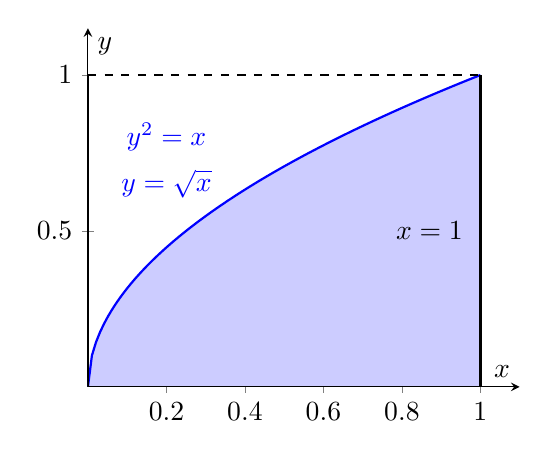
\begin{tikzpicture}
  \begin{axis}[
      axis lines = middle,
      xlabel = $x$, ylabel = $y$,
      domain=0:1,
      ymin=0, ymax=1.15,
      xmin=0, xmax=1.1,
      samples=100,
      clip=true,
      scale=0.8
    ]
    
    \addplot [
      name path=A,
      domain=0:1,
      draw=none,
    ] {sqrt(x)};

    \path[name path=B] (axis cs:0,1) -- (axis cs:1,1);
    \path[name path=C] (axis cs:0,0) -- (axis cs:0,1);
    \path[name path=D] (axis cs:0,0) -- (axis cs:1,0);

    \addplot [fill=blue!20, draw=none] fill between [of=D and A, soft clip={domain=0:1}];
    
    \addplot[blue, thick] {sqrt(x)};
    \addplot[thick] coordinates {(0,0) (0,1)};
    \addplot[thick] coordinates {(1,0) (1,1)};
    \addplot[thick] coordinates {(0,0) (1,0)};
    \draw[dashed] (axis cs: 0,1) -- (axis cs: 1,1);
    \node at (axis cs: 0.87, 0.5) {$x=1$};
    \node[blue] at (axis cs: 0.2, 0.8) {$y^2=x$};
    \node[blue] at (axis cs: 0.2, 0.65) {$y=\sqrt{x}$};

  \end{axis}
\end{tikzpicture}
\end{center}\begin{align*}
\int_0^1\int_{y^2}^1y^3\cos\left(x^3\right)\,dx\,dy&=\int_0^1\int_0^{\sqrt x}y^3\cos\left(x^3\right)\,dy\,dx=\int_0^1\cos\left(x^3\right)\left[\frac{y^4}4\right]_{y=0}^{y=\sqrt x}\,dx\\[1em]&=\frac14\int_0^1x^2\cos\left(x^3\right)\,dx=\frac1{12}\bigg[\sin\left(x^3\right)\bigg]_0^1=\boxed{\frac1{12}\sin1}\end{align*}

\item\begin{enumerate}[leftmargin=*,label=\textbf{\alph*.}]
\item\leavevmode

\begin{minipage}{0.5\textwidth}
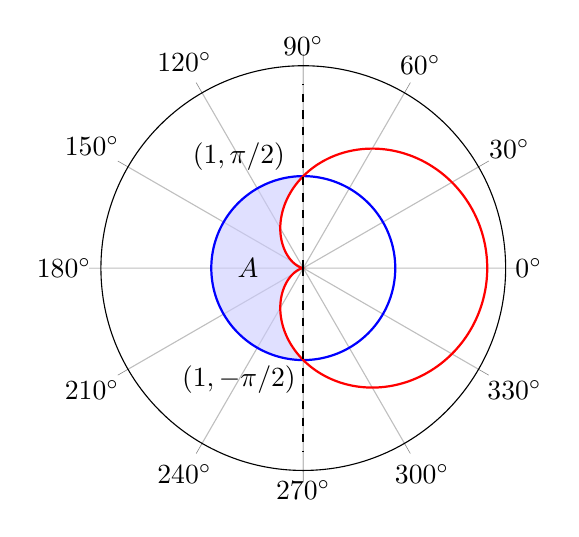
\begin{tikzpicture}
  \begin{polaraxis}[ytick=\empty, axis y line=none, scale=0.75, xticklabel=$\pgfmathprintnumber{\tick}^\circ$,]
    \addplot [
      domain=pi/2:3*pi/2,
      samples=300,
      draw=none,
      name path=A,
      data cs=polarrad,
    ] {1};

    \addplot [
      domain=pi/2:3*pi/2,
      samples=300,
      draw=none,
      name path=B,
      data cs=polarrad,
    ] {1+cos(deg(x))};

    \addplot [
      blue!20,
      fill opacity=0.6,
    ] fill between[of=A and B];

    \addplot [
      domain=0:2*pi,
      samples=300,
      thick,
      blue,
      data cs=polarrad,
    ] {1};

    \addplot [
      domain=0:2*pi,
      samples=300,
      thick,
      red,
      data cs=polarrad,
    ] {1+cos(deg(x))};

    \draw[black, thick, dashed] (axis cs: 90,0) -- (axis cs: 90,2);
    \draw[black, thick, dashed] (axis cs: -90,0) -- (axis cs: -90,2);

    \node at (axis cs:120,1.4) {$(1,\pi/2)$};
    \node at (axis cs:-120,1.4) {$(1,-\pi/2)$};
    \node at (0,-0.6) {$A$};

  \end{polaraxis}
\end{tikzpicture}
\end{minipage}\hfill
\begin{minipage}{0.4\textwidth}
\item\leavevmode
\vspace{-2em}
\[
\boxed{A=\int_{\pi/2}^{3\pi/2}\int_{1+\cos\theta}^1r\,dr\,d\theta}
\]
\end{minipage}
\end{enumerate}

\newpage

\item\begin{enumerate}[leftmargin=*,label=\textbf{\alph*.}]
\item\leavevmode

\begin{minipage}{0.45\textwidth}
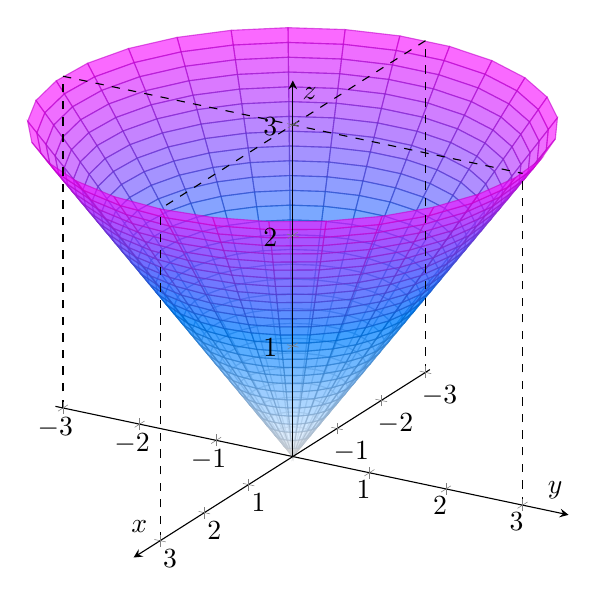
\begin{tikzpicture}
  \begin{axis}[
    view={120}{30},
    axis on top,
    axis lines=center,
    xlabel={$x$},
    ylabel={$y$},
    zlabel={$z$},
    xtick={-3,-2,-1,1,2,3},
    ytick={-3,-2,-1,1,2,3},
    xmin=-3.1, xmax=3.6,
    ymin=-3.1, ymax=3.6,
    zmin=0, zmax=3.4,
    samples=30,
    domain=0:360,
    y domain=0:3,
    scale=1.5,
  ]
  
\addplot3[surf, colormap/cool, z buffer=sort, opacity=0.6] ({y*cos(x)}, {y*sin(x)}, {y});

\draw[dashed] (axis cs:0,-3,3) -- (axis cs:0,3,3);
\draw[dashed] (axis cs:-3,0,3) -- (axis cs:3,0,3);

\draw[dashed] (axis cs:-3,0,0) -- (axis cs:-3,0,3);
\draw[dashed] (axis cs:0,3,0) -- (axis cs:0,3,3);
\draw[dashed] (axis cs:3,0,0) -- (axis cs:3,0,3);
\draw[dashed] (axis cs:0,-3,0) -- (axis cs:0,-3,3);

\end{axis}
\end{tikzpicture}
\end{minipage}\hfill
\begin{minipage}{0.5\textwidth}
\vspace{-3.5em}
\[A=\iint_D\sqrt{1+\left(\frac{\partial z}{\partial x}\right)^2 +\left(\frac{\partial z}{\partial y}\right)^2}\,dA\]
\end{minipage}

\begin{align*}
A&=\iint_D\sqrt{1+\left(\frac{x}{\sqrt{x^2+y^2}}\right)^2 +\left(\frac{y}{\sqrt{x^2+y^2}}\right)^2}\,dA\\[1em]&=\iint_D\sqrt{1+\left(\frac{x^2+y^2}{x^2+y^2}\right)}\,dA=\iint_D\sqrt{1+1}\,dA=\sqrt{2}\iint_D\,dA
\end{align*}

\item If we switch to polar coordinates, we can easily evaluate the integral.
\[A=\sqrt2\int_0^{2\pi}\int_0^3\,r\,dr\,d\theta=\sqrt2\int_0^{2\pi}\left[\frac{r^2}2\right]_{r=0}^{r=3}\,d\theta=\sqrt2\int_0^{2\pi}\frac92\,d\theta=\boxed{9\pi\sqrt2}\]
\end{enumerate}

\item
\begin{enumerate}[leftmargin=*,label=\textbf{\alph*.}]
\item For spherical coordinates, we have
\refstepcounter{equation}
\label{eq:19_20_summer_final_1}
\[
\begin{array}{c}
z=\rho\cos\phi\\
r=\rho\sin\phi\\
x^2+y^2+z^2=\rho^2\\
dV=\rho^2\sin\phi\,d\rho\,d\phi\,d\theta
\end{array}
\quad\longrightarrow\quad
\begin{aligned}
z=8-x^2-y^2
&\implies \rho\cos\phi=8-\rho^2\sin^2\phi\\[0.2cm]
z=x^2+y^2
&\implies \rho\cos\phi=\rho^2\sin^2\phi
\end{aligned}
\quad
\vcenter{\hbox{(\theequation)}}
\]

Now, notice that we have two distinct upper bounds for $\rho$. From $\phi=0$ to the angle of intersection, the integration is bounded above by $z=8-x^2-y^2$, where from the angle of intersection to $\phi=\pi/2$, the integration is bounded above by $z=x^2+y^2$.

Solve the first equation in \eqref{eq:19_20_summer_final_1} for $\rho$ to find the upper bound.
\[\rho\cos\phi=8-\rho^2\sin^2\phi\implies\rho^2\sin^2\phi+\rho\cos\phi-8=0\]

\[\rho_{1,2}=\frac{-\cos\phi\pm\sqrt{\cos^2\phi-4\sin^2\phi\cdot(-8)}}{2\sin^2\phi}\quad\left[x_{1,2}=\frac{-b\pm\sqrt{b^2-4ac}}{2a}\right]\]

\[\rho>0\implies \rho_{\text{upper, 1}}=\frac{-\cos\phi+\sqrt{\cos^2\phi+32\sin^2\phi}}{2\sin^2\phi}\]

Solve the second equation in \eqref{eq:19_20_summer_final_1} for $\rho$ to find the other upper bound.
\[\rho\cos\phi=\rho^2\sin^2\phi\implies\rho_{\text{upper, 2}}=\frac{\cos\phi}{\sin^2\phi}=\cot\phi\csc\phi\]

Find where two surfaces intersect by equating the equations in \eqref{eq:19_20_summer_final_1}.
\[8-\rho^2\sin^2\phi=\rho^2\sin^2\phi\implies \rho^2\sin^2\phi=4\implies \rho\sin\phi=2\implies r=2\]
\[z=x^2+y^2=r^2\implies z=4\implies \rho=\sqrt{x^2+y^2+z^2}=2\sqrt5\]
\[\implies \sin\phi=\frac2\rho=\frac1{\sqrt{5}}\implies\phi=\arcsin\frac1{\sqrt5}\]

We know $0\leq\theta\leq2\pi$. Therefore, the volume in spherical coordinates is as follows.
\[
\boxed{\begin{array}{ll}
V=&\displaystyle\int_0^{2\pi}\int_0^{\arcsin\textstyle\frac1{\sqrt5}}\int_0^{\textstyle\frac{-\cos\phi+\sqrt{\cos^2\phi+32\sin^2\phi}}{2\sin^2\phi}}\rho^2\sin\phi\,d\rho\,d\phi\,d\theta\\[1em]
&\displaystyle+\int_0^{2\pi}\int_{\arcsin\textstyle\frac1{\sqrt5}}^{\pi/2}\int_0^{\cot\phi\csc\phi}\rho^2\sin\phi\,d\rho\,d\phi\,d\theta
\end{array}}
\]

Since we choose the minimum of the bounds for $\rho$, we can write the equivalent expression.
\[\boxed{V=\displaystyle\int_0^{2\pi}\int_0^{\pi/2}\int_0^{\min\left(\cot\phi\csc\phi,\textstyle\frac{-\cos\phi+\sqrt{\cos^2\phi+32\sin^2\phi}}{2\sin^2\phi}\right)}\rho^2\sin\phi\,d\rho\,d\phi\,d\theta}\]

\item For cylindrical coordinates, we have

\refstepcounter{equation}
\label{eq:19_20_summer_final_2}

\[
\begin{array}{c}
z=z\\
r^2=x^2+y^2\\
dV=r\,dz\,dr\,d\theta
\end{array}
\quad\longrightarrow\quad
\begin{aligned}
z=8-x^2-y^2
&\implies z=8-r^2\\[1em]
z=x^2+y^2
&\implies z=r^2
\end{aligned}
\quad
\vcenter{\hbox{(\theequation)}}
\]

Equate the equations in \eqref{eq:19_20_summer_final_2} to find the upper bound for $r$.
\[8-r^2=r^2\implies r^2=4\implies r_{\text{upper}}=2\]

The lower bound for $r$ is 0, and $0\leq\theta\leq2\pi$. The volume can be expressed as follows.
\[\boxed{V=\int_0^{2\pi}\int_0^2\int_{r^2}^{8-r^2}r\,dz\,dr\,d\theta}\]

\end{enumerate}
\end{enumerate}

\newpage
\stepcounter{subsection}
\phantomsection
\addcontentsline{toc}{subsection}{\protect\numberline{\thesubsection}Final - Spring 2021 Solutions}

\fancyhead[R]{\textit{2020-2021 Spring Final}}

%Last update: 05/08/2025 00:46

\begin{enumerate}[leftmargin=*,label=\textbf{\arabic*.}]
\item\leavevmode

\vspace{-1em}
\begin{minipage}{0.48\textwidth}
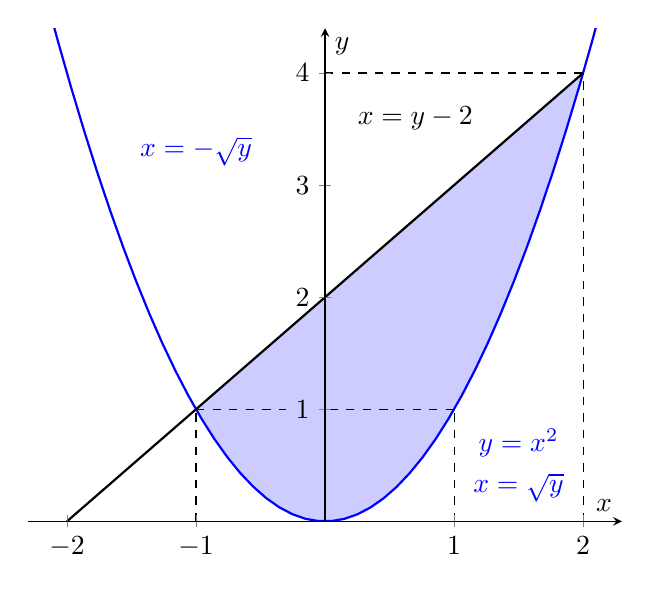
\begin{tikzpicture}
  \begin{axis}[
      axis lines = middle,
      xlabel = $x$, ylabel = $y$,
      ymin=0, ymax=4.4,
      xmin=-2.3, xmax=2.3,
      samples=100,
      clip=true,
      axis on top,
      scale=1.1,
    ]
    
    \addplot [
      name path=A,
      domain=-2:2,
      draw=none,
    ] {x^2};

    \path[name path=B] (axis cs:-1,1) -- (axis cs:2,4);

    \addplot [
      fill=blue!20,
      draw=none,
    ] fill between [
      of=A and B,
      soft clip={domain=-1:2},
    ];
    
    \addplot[blue, thick] {x^2};
    \addplot[black, thick] coordinates {(-2,0) (2,4)};
    \draw[dashed] (axis cs:-1,1) -- (axis cs: -0.3,1);
    \draw[dashed] (axis cs:1,1) -- (axis cs: 0,1);
    \draw[dashed] (axis cs:2,0) -- (axis cs: 2,4);
    \draw[dashed] (axis cs:-1,0) -- (axis cs: -1,1);
    \draw[dashed] (axis cs:1,0) -- (axis cs: 1,1);
    \draw[dashed] (axis cs:0,4) -- (axis cs: 2,4);
    \node[blue] at (axis cs: 1.5, 0.7) {$y=x^2$};
    \node[blue] at (axis cs: 1.5, 0.3) {$x=\sqrt{y}$};
    \node[blue] at (axis cs: -1, 3.3) {$x=-\sqrt{y}$};
    \node at (axis cs: 0.7, 3.6) {$x=y-2$};

  \end{axis}
\end{tikzpicture}
\end{minipage}
\begin{minipage}{0.52\textwidth}
\[
\boxed{\int_0^1\int_{-\sqrt y}^{\sqrt y}\,dx\,dy+\int_1^4\int_{y-2}^{\sqrt y}\,dx\,dy}\]
\end{minipage}

\item Using polar coordinates, we can find the volume with a double integral.
\[
\begin{array}{c}
r^2=x^2+y^2\\
dA=r\,dr\,d\theta
\end{array}\quad\rightarrow\quad
\begin{array}{c}z=\sqrt{x^2+y^2}\implies z=\sqrt{r^2}\implies z=r\\[0.3cm]
x^2+y^2\leq4\,\rightarrow\,r^2\leq4\implies 0\leq r\leq 2\\[0.3cm]
0\leq\theta\leq2\pi
\end{array}
\]
\begin{align*}\text{Volume}&=\int_0^{2\pi}\int_{0}^{2}\left[r-0\right]\cdot r\,dr\,d\theta=\int_0^{2\pi}\int_{0}^{2}r^2\,dr\,d\theta=\int_0^{2\pi}\left[\frac{r^3}3\right]_{r=0}^{r=2}d\theta\\[1em]&=\frac83\int_0^{2\pi}\,d\theta=\boxed{\frac{16\pi}3}\end{align*}

\item\begin{enumerate}[leftmargin=*,label=\textbf{\alph*.}]
\item The region is inside the cardioid and outside the circle.

\begin{minipage}{0.52\textwidth}
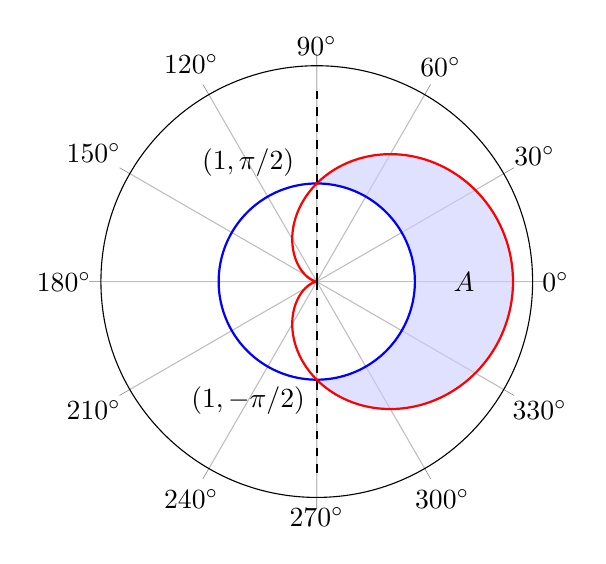
\begin{tikzpicture}
  \begin{polaraxis}[ytick=\empty, axis y line=none, scale=0.8, xticklabel=$\pgfmathprintnumber{\tick}^\circ$,]
    \addplot [
      domain=-pi/2:pi/2,
      samples=300,
      draw=none,
      name path=A,
      data cs=polarrad,
    ] {1};

    \addplot [
      domain=-pi/2:pi/2,
      samples=300,
      draw=none,
      name path=B,
      data cs=polarrad,
    ] {1+cos(deg(x))};

    \addplot [
      blue!20,
      fill opacity=0.6,
    ] fill between[of=A and B];

    \addplot [
      domain=0:2*pi,
      samples=300,
      thick,
      blue,
      data cs=polarrad,
    ] {1};

    \addplot [
      domain=0:2*pi,
      samples=300,
      thick,
      red,
      data cs=polarrad,
    ] {1+cos(deg(x))};

    \draw[black, thick, dashed] (axis cs: 90,0) -- (axis cs: 90,2);
    \draw[black, thick, dashed] (axis cs: -90,0) -- (axis cs: -90,2);

    \node at (axis cs:120,1.4) {$(1,\pi/2)$};
    \node at (axis cs:-120,1.4) {$(1,-\pi/2)$};
    \node at (0,1.5) {$A$};

  \end{polaraxis}
\end{tikzpicture}
\end{minipage}
\begin{minipage}{0.35\textwidth}
\item\leavevmode
\vspace{-3em}
\[\quad\boxed{A=\int_{-\pi/2}^{\pi/2}\int_1^{1+\cos\theta}r\,dr\,d\theta}\]
\end{minipage}
\end{enumerate}

\newpage

\item\begin{enumerate}[leftmargin=*,label=\textbf{\alph*.}]
\item Parabolic cylinder
\begin{center}
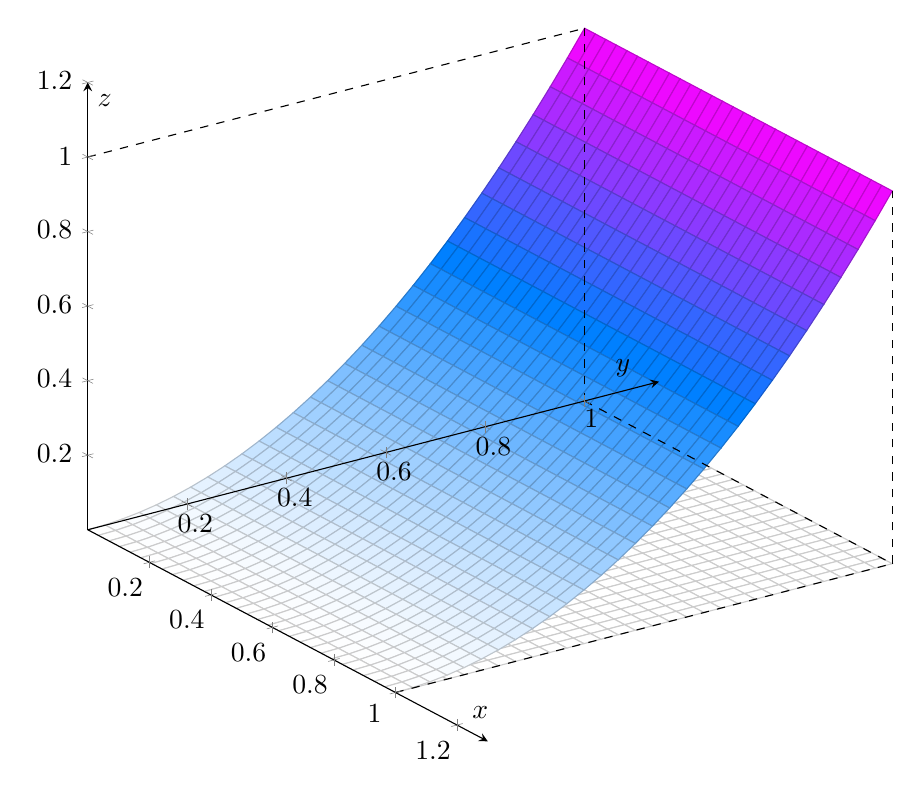
\begin{tikzpicture}
  \begin{axis}[
      view={55}{30},
      axis lines=center,
      xlabel=$x$, ylabel=$y$, zlabel=$z$,
      xmin=0, xmax=1.3,
      ymin=0, ymax=1.15,
      zmin=0, zmax=1.2,
      samples=30,
      domain=0:1,
      y domain=0:1,
      colormap/cool,
      mesh/ordering=y varies,
      scale=1.8,
      axis on top,
    ]
    
    \addplot3[surf]{0};
    \addplot3[surf]{y^2};

    \draw[dashed] (axis cs:0,1,0)--(axis cs:0,1,1);
    \draw[dashed] (axis cs:1,0,0)--(axis cs:1,1,0);
    \draw[dashed] (axis cs:0,1,0)--(axis cs:1,1,0);
    \draw[dashed] (axis cs:1,1,0)--(axis cs:1,1,1);
    \draw[dashed] (axis cs:0,0,1)--(axis cs:0,1,1);

   \end{axis}
\end{tikzpicture}
\end{center}

\item Calculate the partial derivatives to find the surface area.
\[z=y^2\implies\quad\frac{\partial z}{\partial x}=0,\quad \frac{\partial z}{\partial y}=2y\]

Let $S$ be the surface area.
\begin{align*}S&=\iint_D\sqrt{1+\left(\frac{\partial z}{\partial x}\right)^2+\left(\frac{\partial z}{\partial y}\right)^2}\,dA=\int_0^1\int_0^1\sqrt{1+\left(0\right)^2+\left(2y\right)^2}\,dx\,dy\\[1em]&=\int_0^1\int_0^1\sqrt{4y^2+1}\,dx\,dy=\int_0^1\left[x\sqrt{4y^2+1}\right]_{x=0}^{x=1}\,dy\\[1em]&=\int_0^1\sqrt{4y^2+1}\,dy\:\left[y=\frac12\tan u \implies dy=\frac12\sec^2u\,du,\:\begin{array}{l}u_{\text{upper}}=\arctan2\\u_{\text{lower}}=0\end{array}\right]\\[1em]&=\frac12\int_0^{\arctan2}\sqrt{\tan^2u+1}\cdot\sec^2u\,du=\frac12\int_0^{\arctan2}\sec^3u\,du\end{align*}

To evaluate the last integral, we will use integration by parts.
\begin{align*}
    w=\sec u\,&\rightarrow\, dw = \sec u\tan u \,du\\
    dz=\sec^2u\,du\,&\rightarrow\, z = \tan u
\end{align*}
\begin{align*}
\int_0^{\arctan2}\sec^3u\,du&=\tan u \cdot \sec u\,\bigg|_0^{\arctan2} -\int_0^{\arctan2} \tan^2 u\sec u\, du\\[1em]&= \tan u \cdot \sec u\,\bigg|_0^{\arctan2} -\int_0^{\arctan2} \frac{1-\cos^2u}{\cos^3 u}\, du\\[1em]&= \tan u \cdot \sec u\,\bigg|_0^{\arctan2} - \int_0^{\arctan2} \sec^3u \, du + \int_0^{\arctan2} \sec u \, du 
\end{align*}

Notice that the integral we want to evaluate appears on the right side. After a little algebra, we can evaluate the integral.
\[\int_0^{\arctan2}\sec^3u\,du=\frac12\cdot\tan u\cdot\sec u\,\bigg|_0^{\arctan2}+\frac12\cdot\int_0^{\arctan2}\sec u\,du\]

The integral of $\sec u$ with respect to $u$ is as follows. One can derive it with particular methods.
\[\int_0^{\arctan2}\sec u \, du = \ln\left|\tan u + \sec u\right|\bigg|_0^{\arctan2}\]

So, the surface area becomes as follows.
\begin{align*}S&=\frac12\int_0^{\arctan2}\sec^3u\,du=\frac14\left(\tan u\cdot\sec u+\ln\left|\tan u+\sec u\right|\right)\bigg|_0^{\arctan2}\\[1em]&=\frac14\left[2\sec(\arctan2)+ \ln(2+\sec(\arctan2))-0\right]=\boxed{\frac14\left[2\sqrt5+\ln\left(2+\sqrt5\right)\right]}\end{align*}
\end{enumerate}

\item We can easily evaluate the integral with spherical coordinates,
\[
\begin{array}{c}
z=\rho\cos\theta\\
r=\rho\sin\theta\\
x^2+y^2+z^2=\rho^2\\
dV=\rho^2\sin\phi\,d\rho\,d\phi\,d\theta
\end{array}\quad\rightarrow\quad
\begin{array}{c}
x^2+y^2+z^2=4\,\rightarrow\,\rho^2 = 4\implies \rho_{\text{min}}=2\\
x^2+y^2+z^2=9\,\rightarrow\,\rho^2 = 9\implies \rho_{\text{max}}=3\\
z\equiv\rho\cos\phi\\
0\leq\theta\leq2\pi,\quad0\leq\phi\leq\pi
\end{array}
\]

\begin{align*}
\iiint_Ez\,dV&=\int_0^{2\pi}\int_0^\pi\int_2^3\rho\cos\phi\cdot\rho^2\sin\phi\,d\rho\,d\phi\,d\theta=\frac12\int_0^{2\pi}\int_0^\pi\int_2^3\rho^3\sin(2\phi)\,d\rho\,d\phi\,d\theta\\[1em]&=\frac12\int_0^{2\pi}\int_0^\pi\left[\frac{\rho^4}{4}\right]_{\rho=2}^{\rho=3}\sin(2\phi)\,d\phi\,d\theta=\frac{65}{8}\int_0^{2\pi}\int_0^\pi\sin(2\phi)\,d\phi\,d\theta\\[1em]&=\frac{65}{8}\int_0^{2\pi}\left[-\frac12\cos(2\phi)\right]_{\phi=0}^{\phi=\pi}\,d\theta=\frac{65}{8}\int_0^{2\pi}0\,d\theta =\boxed0
\end{align*}

\newpage

\item \begin{enumerate}[leftmargin=*,label=\textbf{\alph*.}]
\item For spherical coordinates, we have
\refstepcounter{equation}
\label{eq:20_21_spring_final_1}
\[
\begin{array}{c}
z=\rho\cos\phi\\
r=\rho\sin\phi\\
x^2+y^2+z^2=\rho^2\\
dV=\rho^2\sin\phi\,d\rho\,d\phi\,d\theta
\end{array}
\quad\rightarrow\quad
\begin{array}{cc}
z=1-x^2-y^2
\implies
\rho\cos\phi=1-\rho^2\sin^2\phi
\\[1em]
\displaystyle
0\leq\phi\leq\frac{\pi}{2},
\quad
0\leq\theta\leq2\pi,
\quad
0\leq\rho\leq\rho_{\text{upper}}
\end{array}
\hfill
\vcenter{\hbox{(\theequation)}}
\]

Find $\rho_{\text{upper}}$ with the equation in \eqref{eq:20_21_spring_final_1}.
\[
\begin{array}{c}
\rho\cos\phi=1-\rho^2\sin^2\phi\implies \rho^2\sin^2\phi+\rho\cos\phi-1=0\\\\
\displaystyle \rho_{1,2} = \frac{-\cos\phi \pm\sqrt{\cos^2\phi-4\cdot\sin^2\phi\cdot(-1)}}{2\sin^2\phi}\quad\left[x_{1,2}=\frac{-b\pm\sqrt{b^2-4ac}}{2a}\right]\\\\
\displaystyle \rho>0\implies\rho_{\text{upper}}=\frac{-\cos\phi +\sqrt{\cos^2\phi+4\sin^2\phi}}{2\sin^2\phi}
\end{array}
\]

\[\boxed{\text{Volume}=\int_0^{2\pi}\int_0^{\pi/2}\int_0^{\textstyle\frac{-\cos\phi +\sqrt{\cos^2\phi+4\sin^2\phi}}{2\sin^2\phi}}\rho^2\sin\phi\,d\rho\,d\phi\,d\theta}\]

\item For cylindrical coordinates, we have
\[
\begin{array}{c}
z=z\\
r^2=x^2+y^2\\
dV=r\,dz\,dr\,d\theta
\end{array}\quad\rightarrow\quad
\begin{array}{c}
z=1-x^2-y^2\implies z=1-r^2\\
0\leq\theta\leq2\pi,\quad 0\leq r \leq1
\end{array}
\]

\[\boxed{\text{Volume}=\int_0^{2\pi}\int_0^1\int_0^{1-r^2}r\,dz\,dr\,d\theta}\]
\end{enumerate}
\end{enumerate}

\newpage
\stepcounter{subsection}
\phantomsection
\addcontentsline{toc}{subsection}{\protect\numberline{\thesubsection}Final - Spring 2022 Solutions}

\fancyhead[R]{\textit{2021-2022 Spring Final}}

%Last update: 05/08/2025 01:58

\begin{enumerate}[leftmargin=*,label=\textbf{\arabic*.}]
\item Let $g(x,y)=x+y-1$ and then, solve the system of equations below using the method of Lagrange multipliers.
\[
\left.
\begin{array}{ll}
\displaystyle\nabla f =\lambda \nabla g \\
\displaystyle g(x,y) = 0
\end{array}
\right\}\quad
\begin{array}{ll}
\nabla f = \left\langle 2x, 2y\right\rangle = \lambda\left\langle1,1\right\rangle = \lambda\nabla g\\\therefore\displaystyle \lambda = 2x\quad \text{and}\quad \lambda = 2y\quad \text{and}\quad x+y-1=0
\end{array}
\]
\[\lambda=2x=2y\implies x=y\]
\[x+y-1=0 \,\rightarrow\, 2x-1 = 0\,\rightarrow\,x=\frac12=y\]
Evaluate $f\left(\frac12,\frac12\right)$ to find the minimum value.
\[f\left(\frac12,\frac12\right)=\left(\frac12\right)^2+\left(\frac12\right)^2=\frac12\]

$f(x,y)$ is defined for $x\geq0$ and $y\geq0$. This implies that $0\leq y \leq1$ and $0\leq x\leq1$ by the constraint. The domain of $f$ is closed and bounded, and $f$ is continuous. By the extreme value theorem, the absolute minima and maxima must exist. Using the method of Lagrange multipliers, we could find only one point. This means that the other value exists on the boundary of $f$.
\[x=0\,\rightarrow\,0+y-1=0\,\rightarrow\,y=1,\quad y=0\,\rightarrow\, x+0-1=0\,\rightarrow\, x=1\]
\[f(0,1) = 0^2 +1^2 = 1,\quad f(1,0) = 1^2+0^2 = 1\]

Eventually, compare the values we obtain.
\[\boxed{\frac12\,\text{is the absolute minimum}, 1\,\text{is the absolute maximum}.}\]

\item\leavevmode
\vspace{-1em}
\begin{center}
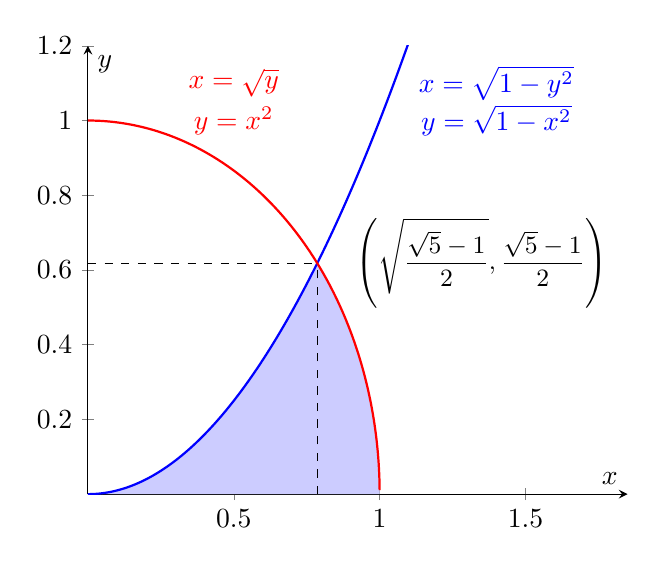
\begin{tikzpicture}
  \begin{axis}[
      axis lines=center,
      xlabel={$x$},
      ylabel={$y$},
      xmin=0, xmax=1.85,
      ymin=0, ymax=1.2,
      samples=200,
      clip=true,
      scale=1,
    ]
    
    \addplot [
        fill=blue!20,
        domain=0:0.786,
        draw=none,
    ] {x^2} \closedcycle;
    
    \addplot [
        fill=blue!20,
        domain=0.784:1,
        draw=none,
    ] {sqrt(1-x^2)} \closedcycle;

    \addplot [
        thick,
        blue,
        domain=0:1.1,
        samples=200,
    ] {x^2};

    \addplot [
        thick,
        red,
        domain=0:1.1,
        samples=3200,
    ] {sqrt(1-x^2)};

    \node[blue] at (axis cs:1.4,1.1) {$x = \sqrt{1 - y^2}$};
    \node[red] at (axis cs:0.5,1.1) {$x = \sqrt{y}$};
    \node[blue] at (axis cs:1.4,1) {$y = \sqrt{1 - x^2}$};
    \node[red] at (axis cs:0.5,1) {$y=x^2$};
    \node at (axis cs:1.35,0.618) {\small$\displaystyle\left(\sqrt{\frac{\sqrt5-1}{2}},\frac{\sqrt5-1}2\right)$};

    % Label y-max
    \draw[dashed] (axis cs:0,0.618) -- (axis cs:{sqrt(0.618)},0.618);
    \draw[dashed] (axis cs:0.786,0) -- (axis cs:0.786,0.618);

    \node[left] at (axis cs:0,0.618) {\footnotesize $\frac{-1+\sqrt{5}}{2}$};

  \end{axis}
\end{tikzpicture}
\end{center}

The integral with reverse order is as follows.
\[\boxed{\int_0^{\sqrt{\frac{\sqrt5 - 1}2}}\int_0^{x^2}\,dy\,dx + \int_{\sqrt{\frac{\sqrt5 - 1}2}}^{1}\int_0^{\sqrt{1-x^2}}\,dy\,dx}\]

\item Find where these two curves intersect and then find the area.
\[1=1+\sin\theta\implies\sin\theta=0\implies\theta=k\pi,\quad k\in\mathbb{Z}\]

\begin{center}
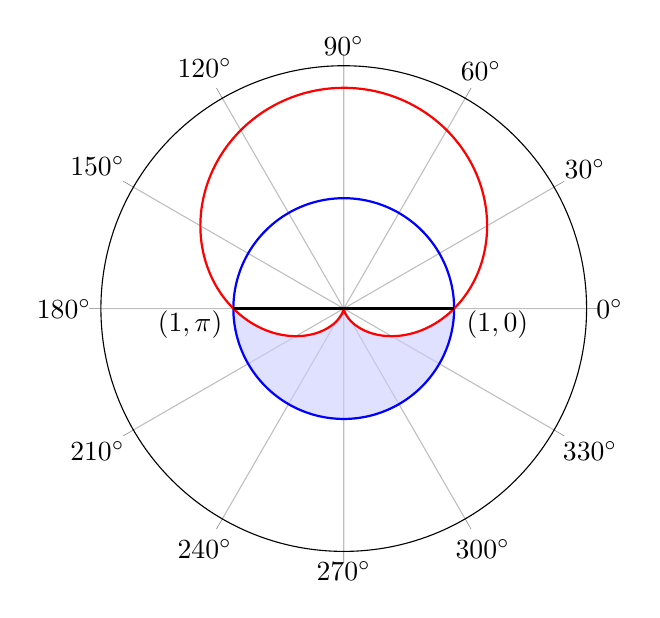
\begin{tikzpicture}
  \begin{polaraxis}[ytick=\empty, axis y line=none, xticklabel=$\pgfmathprintnumber{\tick}^\circ$, scale=0.9]
    \addplot [
      domain=pi:2*pi,
      samples=300,
      draw=none,
      name path=A,
      data cs=polarrad,
    ] {1};

    \addplot [
      domain=pi:2*pi,
      samples=300,
      draw=none,
      name path=B,
      data cs=polarrad,
    ] {1+sin(deg(x))};

    \addplot [
      blue!20,
      fill opacity=0.6,
    ] fill between[of=A and B];

    \addplot [
      domain=0:2*pi,
      samples=300,
      thick,
      blue,
      data cs=polarrad,
    ] {1};

    \addplot [
      domain=0:2*pi,
      samples=300,
      thick,
      red,
      data cs=polarrad,
    ] {1+sin(deg(x))};

    \draw[black, thick] (axis cs: 0,-1) -- (axis cs: 0,1);
    \node at (axis cs: 6,-1.4) {$(1,\pi)$};
    \node at (axis cs: -6,1.4) {$(1,0)$};

  \end{polaraxis}
\end{tikzpicture}
\end{center}
\begin{align*}
\text{Area}&=\int_{\pi}^{2\pi}\int_{1+\sin\theta}^1\,r\,dr\,d\theta=\frac12\int_\pi^{2\pi}\left[1^2-(1+\sin\theta)^2\right]\,d\theta\\[1em]&=\frac12\int_\pi^{2\pi}\left[-2\sin\theta-\sin^2\theta\right]\,d\theta\quad\left[\sin^2\theta+\cos^2\theta=1\right]\\[1em]&=-\int_\pi^{2\pi}\sin\theta\,d\theta-\frac12\int_\pi^{2\pi}(1-\cos^2\theta)\,d\theta\quad[2\cos^2\theta-1=\cos(2\theta)] \\[1em]&=-\int_\pi^{2\pi}\sin\theta\,d\theta+\int_\pi^{2\pi}\frac{\cos(2\theta)-1}{4}\,d\theta=\int_\pi^{2\pi}\left[-\frac14+\frac14\cos(2\theta)-\sin\theta\right]\,d\theta\\[1em]&=\left[-\frac\theta4+\frac18\sin(2\theta)+\cos\theta\right]_{\pi}^{2\pi}=\left[\left(-\frac{\pi}2+0+1\right)-\left(-\frac{\pi}4+0-1\right)\right]={\boxed{2-\frac{\pi}4}}
\end{align*}

\item We have the sphere $x^2+y^2+z^2=16$. So, the upper bound is $z=\sqrt{16-x^2-y^2}$, while the lower bound is $z=0$. If we project the domain onto the $xy$-plane, we see that the upper and lower bounds for $y$ are $\sqrt{2-x^2}$ and $-\sqrt{2-x^2}$, respectively. For $x$, the integration starts from $-\sqrt2$ and ends at $\sqrt2$. The volume of the object can be evaluated using the following integral.

\newpage
\[{I}=\int_{-\sqrt2}^{\sqrt2}\int_{-\sqrt{2-x^2}}^{\sqrt{2-x^2}}\left[\sqrt{16-x^2-y^2}-0 \right]\,dy\,dx\]
This integral seems a little bit hard. We can switch to polar coordinates for ease. Use the transformation below.
\[
\begin{array}{c}
x^2+y^2=r^2\\
dA=dy\,dx =r\,dr\,d\theta
\end{array}\quad\rightarrow\quad
\begin{array}{c}
0\leq z\leq\sqrt{16-r^2}\\
0\leq r\leq \sqrt2\\
0\leq\theta\leq 2\pi\\
\end{array} 
\]
\begin{align*}{I}&=\int_{0}^{2\pi}\int_{0}^{\sqrt{2}}\sqrt{16-r^2}\,r\,dr\,d\theta=\int_{0}^{2\pi}\left[-\frac13\left(16-r^2\right)^{3/2}\right]_{r=0}^{r=\sqrt2}\,d\theta\\[1em]&=\frac13\int_0^{2\pi}\left[-14^{3/2}-\left(-16^{3/2}\right)\right]\,d\theta=\boxed{\frac{2\pi}{3}\left(16^{3/2}-14^{3/2}\right)}
\end{align*}

\item \begin{enumerate}[leftmargin=*,label=\textbf{\alph*.}]
\item\leavevmode
\begin{center}
\begin{tikzpicture}
  \begin{axis}[
    view={125}{30},
    axis lines=center,
    xlabel={$x$},
    ylabel={$y$},
    zlabel={$z$},
    xtick={-2,-1,1,2},
    ytick={-2,-1,1,2},
    xmin=-2, xmax=2.5,
    ymin=-2, ymax=2.5,
    zmin=0, zmax=2.5,
    samples=30,
    domain=0:360,
    colormap/cool,
    scale=1.8,
    axis on top
  ]
    \addplot3[
      surf,
      z buffer=sort,
      y domain=1:2,
    ]
    ({y*cos(x)}, {y*sin(x)}, {y});
%\addplot3[y domain=0:1, dashed, samples = 10]({y*cos(x)}, {y*sin(x)}, {y});
    
\draw[dashed] (axis cs:0,-2,2) -- (axis cs: 0, 2, 2);
\draw[dashed] (axis cs:-2,0,2) -- (axis cs: 2, 0,2);
\draw[dashed] (axis cs:-1,0,1) -- (axis cs: 1, 0, 1);
\draw[dashed] (axis cs:0,-1,1) -- (axis cs: 0, 1,1);

\draw[dashed] (axis cs:-2,0,0) -- (axis cs: -2, 0, 2);
\draw[dashed] (axis cs:0,2,0) -- (axis cs: 0,2,2);
\draw[dashed] (axis cs:2,0,0) -- (axis cs: 2, 0, 2);
\draw[dashed] (axis cs:0,-2,0) -- (axis cs: 0, -2,2);

\draw[dashed] (axis cs:-1,0,0) -- (axis cs: -1, 0, 1);
\draw[dashed] (axis cs:0,1,0) -- (axis cs: 0,1,1);
\draw[dashed] (axis cs:1,0,0) -- (axis cs: 1, 0, 1);
\draw[dashed] (axis cs:0,-1,0) -- (axis cs: 0, -1,1);

\end{axis}
\end{tikzpicture}
\end{center}

\item Using the double integral below, we find the lateral surface area.
\begin{align*}
A&=\iint_D\sqrt{1+\left(\frac{\partial z}{\partial x}\right)^2 +\left(\frac{\partial z}{\partial y}\right)^2}\,dA\\[1em]&=\iint_D\sqrt{1+\left(\frac{x}{\sqrt{x^2+y^2}}\right)^2 +\left(\frac{y}{\sqrt{x^2+y^2}}\right)^2}\,dA \\[1em]&=\iint_D\sqrt{1+\left(\frac{x^2+y^2}{x^2+y^2}\right)}\,dA=\iint_D\sqrt{1+1}\,dA=\sqrt{2}\iint_D\,dA
\end{align*}

\newpage

If we switch to polar coordinates, we can easily evaluate the integral.
\[A=\sqrt2\int_0^{2\pi}\int_1^2\,r\,dr\,d\theta=\sqrt2\int_0^{2\pi}\left[\frac{r^2}2\right]_{r=1}^{r=2}\,d\theta=\sqrt2\int_0^{2\pi}\frac32\,d\theta=\boxed{3\pi\sqrt2}\]
\end{enumerate}

\item \begin{enumerate}[leftmargin=*,label=\textbf{\alph*.}]
\item For spherical coordinates, we have
\[
\begin{array}{c}
z=\rho\cos\phi\\
r=\rho\sin\phi\\
x^2+y^2+z^2=\rho^2\\
dV=\rho^2\sin\phi\,d\rho\,d\phi\,d\theta
\end{array}\quad\rightarrow\quad
\begin{array}{c}
x^2+y^2=1\,\rightarrow\,\rho^2\sin^2\phi = 1\\
z=6\,\rightarrow\,\rho\cos\phi=6\\
z=1-x^2-y^2\,\rightarrow\,\rho\cos\phi=1-\rho^2\sin^2\phi
\end{array}
\]

We have the lower bound for $\rho$, which is the solution of $\rho\cos\phi=1-\rho^2\sin^2\phi$
\[
\begin{array}{c}
\rho\cos\phi=1-\rho^2\sin^2\phi\\[1em]
\rho^2\sin^2\phi+\rho\cos\phi-1=0\\[1em]
\displaystyle \rho_{1,2} = \frac{-\cos\phi \pm\sqrt{\cos^2\phi-4\cdot\sin^2\phi\cdot(-1)}}{2\sin^2\phi}\quad\left[x_{1,2}=\frac{-b\pm\sqrt{b^2-4ac}}{2a}\right]\\[1em]
\displaystyle \rho>0\implies\rho_{\text{lower}}=\frac{-\cos\phi +\sqrt{\cos^2\phi+4\sin^2\phi}}{2\sin^2\phi}
\end{array}
\]

However, we have two distinct upper bounds for $\rho$. We need to find the value of $\phi$ where the surfaces $\rho\cos\phi = 6$ and $\rho^2\sin^2\phi=1$ intersect.
\[\rho^2\sin^2\phi=1 \,\rightarrow\,\rho\sin\phi = 1\]

\[
\left.
\begin{array}{c}
\rho\sin\phi=1\\
\rho\cos\phi=6
\end{array}
\right\}\quad\tan\phi=\frac16\implies\phi=\arctan{\frac16}
\]

For $\displaystyle\phi<\arctan\frac16$, the upper bound is $\displaystyle \frac6{\cos\phi}$. Meanwhile, for $\displaystyle\phi>\arctan\frac16$, it is $\displaystyle \frac1{\sin\phi}$.

The region in the $xy-$plane is circular, therefore $0\leq\theta\leq2\pi$. As for $\phi$, we have $\displaystyle0\leq\phi\leq\frac{\pi}2$. The volume of the object in spherical coordinates can be expressed as follows.

\[
\boxed{\begin{array}{cc}
V=&\displaystyle\int_0^{2\pi}\int_0^{\arctan{\textstyle\frac16}}\int_{\textstyle\frac{-\cos\phi +\sqrt{\cos^2\phi+4\sin^2\phi}}{2\sin^2\phi}}^{\textstyle\frac6{\cos\phi}}\,\rho^2\sin\phi\,d\rho\,d\phi\,d\theta\\
&\displaystyle+\int_0^{2\pi}\int_{\arctan{\textstyle\frac16}}^{\pi/2}\int_{\textstyle\frac{-\cos\phi +\sqrt{\cos^2\phi+4\sin^2\phi}}{2\sin^2\phi}}^{\textstyle\frac1{\sin\phi}}\,\rho^2\sin\phi\,d\rho\,d\phi\,d\theta 
\end{array}}
\]

In fact, we are looking for the minimum value of the upper bound for $\rho$ between $\displaystyle\frac1{\sin\phi}$ and $\displaystyle\frac6{\cos\phi}$. Hence, we can write the equivalent expression as follows.
\[\boxed{V=\displaystyle\int_0^{2\pi}\int_0^{\pi/2}\int_{\textstyle\frac{-\cos\phi +\sqrt{\cos^2\phi+4\sin^2\phi}}{2\sin^2\phi}}^{\min\left(\textstyle\frac6{\cos\phi},\frac1{\sin\phi}\right)}\,\rho^2\sin\phi\,d\rho\,d\phi\,d\theta}\]

\item For cylindrical coordinates, we have
\[
\begin{array}{c}
z=z\\
r^2=x^2+y^2\\
dV=r\,dz\,dr\,d\theta
\end{array}\quad\rightarrow\quad
\begin{array}{c}
x^2+y^2=1\,\rightarrow\,r^2 = 1\,\rightarrow\,r=1\\
z=6\\
z=1-x^2-y^2\,\rightarrow\,z=1-r^2
\end{array}
\]

The volume can be expressed as follows.
\begin{align*}
    V&=\int_0^{2\pi}\int_0^1\int_{1-r^2}^{6}\,r\,dz\,dr\,d\theta=\int_0^{2\pi}\int_0^1\big[z\big]_{z=1-r^2}^{z=6}\,r\,dr\,d\theta\\[1em]&=\int_0^{2\pi}\int_0^1\left(r^3+5r\right)\,dr\,d\theta=\int_0^{2\pi}\left[\frac{r^4}{4} + \frac{5r^2}{2}\right]_{r=0}^{r=1}\,d\theta\\[1em]&=\big[\theta\big]_0^{2\pi}\cdot\left[ \left(\frac{1^4}4 + \frac{5\cdot1^2}2\right)-\left(0\right)\right]=\boxed{\frac{11\pi}2}
\end{align*}

\end{enumerate}
\end{enumerate}

\newpage
\stepcounter{subsection}
\phantomsection
\addcontentsline{toc}{subsection}{\protect\numberline{\thesubsection}Final - Spring 2023 Solutions}

\fancyhead[R]{\textit{2022-2023 Spring Final}}

%Last update: 05/08/2025 00:53

\begin{enumerate}[leftmargin=*,label=\textbf{\arabic*.}]
\item Let $g(x,y,z)=x^2+y^2+z^2-4$ and then solve the system of equations below using the method of Lagrange multipliers.
\[
\left.
\begin{array}{ll}
\displaystyle\nabla f =\lambda \nabla g \\
\displaystyle g(x,y,z) = 0
\end{array}
\right\}\quad
\begin{array}{ll}
\nabla f = \left\langle y^2z,2xyz,xy^2\right\rangle = \lambda\left\langle2x,2y,2z\right\rangle = \lambda\nabla g \\[0.2cm] x^2+y^2+z^2-4=0
\end{array}
\]
\vspace{-2em}
\begin{align}
y^2z &= \lambda\cdot 2x
\label{eq:22_23_spring_final_1}\\
2xyz &= \lambda\cdot 2y
\label{eq:22_23_spring_final_2}\\
xy^2 &= \lambda\cdot 2z
\label{eq:22_23_spring_final_3}
\end{align}
\vspace{-2em}
\begin{align}
\eqref{eq:22_23_spring_final_1}\,\&\,
\eqref{eq:22_23_spring_final_3}
&\rightarrow \frac{z}{x}=\frac{x}{z}
\rightarrow x^2=z^2
\rightarrow x=\pm z
\label{eq:22_23_spring_final_4}\\[0.4cm]
\eqref{eq:22_23_spring_final_1}\,\&\,
\eqref{eq:22_23_spring_final_2}
&\rightarrow \frac{y}{2x}=\frac{x}{y}
\rightarrow y^2=2x^2
\rightarrow y=\pm\sqrt{2}x
\label{eq:22_23_spring_final_5}\\[0.4cm]
\eqref{eq:22_23_spring_final_4}\,\&\,
\eqref{eq:22_23_spring_final_5}
&\rightarrow y=\pm\sqrt{2}z\nonumber
\end{align}
Now, use the constraint to find the coordinates. Write $y$ and $z$ in terms of $x$.
\[x^2+y^2+z^2-4=0\implies x^2+\left(\sqrt2x\right)^2+x^2-4=0\implies4x^2=4\implies x=\pm1\]
\[\therefore y=\pm\sqrt2,\quad z=\pm1\]
 
Evaluate $f$ at either of these points: $(1,\sqrt2,1)$, $(-1,\sqrt2,-1)$, $(-1,-\sqrt2,-1)$.
\[f_{\text{max}}=f(1,\sqrt2,1)=1\cdot\left(\sqrt2\right)^2\cdot1=\boxed{2}\]

\item \leavevmode
\vspace{-2em}
\begin{center}
\begin{tikzpicture}
  \begin{axis}[
      axis lines=center,
      xlabel={$x$},
      ylabel={$y$},
      xmin=0, xmax=1.2,
      ymin=0, ymax=1.2,
      samples=200,
      clip=true,
      scale=0.8,
    ]
    
    \addplot [
        fill=blue!20,
        domain=0:1,
        draw=black,
    ] {1} \closedcycle;
    
    \addplot [
        fill=white,
        domain=0:1,
        draw=black,
    ] {x^(1/4)} \closedcycle;

    \addplot [
        thick,
        blue,
        domain=0:1.1,
    ] {1};

    \addplot [
        thick,
        red,
        domain=0:1.1,
        samples=200,
    ] {x^(1/4)};

    \node[blue] at (axis cs: 0.4, 1.1) {$y=1$};
    \node[red] at (axis cs: 0.4, 0.5) {$y=x^{1/4}$};
    \node[red] at (axis cs: 0.4, 0.35) {$x=y^4$};

  \end{axis}
\end{tikzpicture}
\end{center}

The integral given with this order is difficult to evaluate. Change the order of integration.
\begin{align*}\int_0^1\int_{x^{1/4}}^1\,{e}^{y^5}dy\,dx=\int_0^1\int_0^{y^4}{e}^{y^5}\,dx\,dy=\int_0^1y^4{e}^{y^5}\,dy=\left[\frac15{e}^{y^5}\right]_0^1=\boxed{\frac{{e-1}}{5}}\end{align*}

\item Find where these two curves intersect and then find the area.
\[2-\cos\theta=1+\cos\theta\implies2\cos\theta=1\implies\cos\theta=\frac12\implies\theta=2k\pi\pm\frac{\pi}{3},\quad k\in\mathbb{Z}\]
\begin{center}
\begin{tikzpicture}
  \begin{polaraxis}[ytick=\empty, axis y line=none, scale=0.9, xticklabel=$\pgfmathprintnumber{\tick}^\circ$,]
    \addplot [
      domain=-pi/3:pi/3,
      samples=300,
      draw=none,
      name path=A,
      data cs=polarrad,
    ] {2-cos(deg(x))};

    \addplot [
      domain=-pi/3:pi/3,
      samples=300,
      draw=none,
      name path=B,
      data cs=polarrad,
    ] {1+cos(deg(x))};

    \addplot [
      blue!20,
      fill opacity=0.6,
    ] fill between[of=A and B];

    \addplot [
      domain=0:2*pi,
      samples=300,
      thick,
      blue,
      data cs=polarrad,
    ] {2-cos(deg(x))};

    \addplot [
      domain=0:2*pi,
      samples=300,
      thick,
      red,
      data cs=polarrad,
    ] {1+cos(deg(x))};

    \draw[black, thick] (axis cs: 0,0) -- (axis cs:60,3/2);
    \draw[black, thick] (axis cs: 0,0) -- (axis cs:-60,3/2);
    \node at (axis cs: 45,2.3) {$(3/2,\pi/3)$};
    \node at (axis cs: -45,2.3) {$(3/2,-\pi/3)$};
    
  \end{polaraxis}
\end{tikzpicture}
\end{center}

\vspace{-1em}
Let $A$ be the area.
\begin{align*}
A&=\int_{-\pi/3}^{\pi/3}\int_{2-\cos\theta}^{1+\cos\theta}\,r\,dr\,d\theta=\frac12\int_{-\pi/3}^{\pi/3}\left[(1+\cos\theta)^2-(2-\cos\theta)^2\right]d\theta\\[1em]&=\frac12\int_{-\pi/3}^{\pi/3}\left[1+2\cos\theta+\cos^2\theta-\left(4-4\cos\theta+\cos^2\theta\right)\right]d\theta=\frac12\int_{-\pi/3}^{\pi/3}\left(6\cos\theta-3\right)d\theta \\[1em]&=\frac12\bigg[6\sin\theta-3\theta\bigg]_{-\pi/3}^{\pi/3}=\frac12\left[6\sin\frac\pi3-3\cdot\frac\pi3-\left(6\sin\left(-\frac\pi3\right)+3\cdot\frac{\pi}3 \right)\right]=\boxed{3\sqrt3-\pi}
\end{align*}

\item The upper bound is $z=4-x^2-y^2$, while the lower bound is $z=0$. If we project the domain onto the $xy$-plane, we see that the upper and lower bounds for $y$ are $\sqrt{2-x^2}$ and $0$, respectively. For $x$, the integration starts from $0$ and ends at $\sqrt2$. The volume of the object can be evaluated using the following integral.
\[{I}=\int_0^{\sqrt2}\int_0^{\sqrt{2-x^2}}\left[4-x^2-y^2-0 \right]\,dy\,dx\]

This integral seems a little bit hard. We can switch to polar coordinates for ease.
\[
\begin{array}{c}
x^2+y^2=r^2\\
dA=dy\,dx =r\,dr\,d\theta
\end{array}\quad\rightarrow\quad
\begin{array}{c}
0\leq z\leq4-r^2\\
0\leq r\leq \sqrt2\\
0\leq\theta\leq \pi/2\\
\end{array}
\]

\vspace{-1em}
\begin{align*}{I}&=\int_{0}^{\pi/2}\int_{0}^{\sqrt{2}}\left(4-r^2\right)\,r\,dr\,d\theta=\int_{0}^{\pi/2}\int_{0}^{\sqrt{2}}\left(4r-r^3\right)\,dr\,d\theta\\[1em]&=\int_{0}^{\pi/2}\left[2r^2-\frac{r^4}4\right]_{r=0}^{r=\sqrt2}\,d\theta=\int_0^{\pi/2}3\,d\theta=\boxed{\frac{3\pi}2}
\end{align*}

\item
\begin{enumerate}[leftmargin=*,label=\textbf{\alph*.}]
\item\leavevmode

\vspace{-1em}
\begin{center}
\begin{tikzpicture}
  \begin{axis}[
    view={120}{30},
    axis lines=center,
    xlabel={$x$},
    ylabel={$y$},
    zlabel={$z$},
    xtick={-2,-1,1,2},
    ytick={-2,-1,1,2},
    xmin=-2, xmax=2.5,
    ymin=-2, ymax=2.5,
    zmin=0, zmax=2.5,
    samples=30,
    domain=0:360,
    colormap/cool,
    scale=1.6,
    axis on top
  ]
    \addplot3[
      surf,
      z buffer=sort,
      y domain=1:2,
    ]
    ({y*cos(x)}, {y*sin(x)}, {y});
%\addplot3[y domain=0:1, dashed, samples = 10]({y*cos(x)}, {y*sin(x)}, {y});
    
\draw[dashed] (axis cs:0,-2,2) -- (axis cs: 0, 2, 2);
\draw[dashed] (axis cs:-2,0,2) -- (axis cs: 2, 0,2);
\draw[dashed] (axis cs:-1,0,1) -- (axis cs: 1, 0, 1);
\draw[dashed] (axis cs:0,-1,1) -- (axis cs: 0, 1,1);

\draw[dashed] (axis cs:-2,0,0) -- (axis cs: -2, 0, 2);
\draw[dashed] (axis cs:0,2,0) -- (axis cs: 0,2,2);
\draw[dashed] (axis cs:2,0,0) -- (axis cs: 2, 0, 2);
\draw[dashed] (axis cs:0,-2,0) -- (axis cs: 0, -2,2);

\draw[dashed] (axis cs:-1,0,0) -- (axis cs: -1, 0, 1);
\draw[dashed] (axis cs:0,1,0) -- (axis cs: 0,1,1);
\draw[dashed] (axis cs:1,0,0) -- (axis cs: 1, 0, 1);
\draw[dashed] (axis cs:0,-1,0) -- (axis cs: 0, -1,1);

\end{axis}
\end{tikzpicture}
\end{center}

\item Using the double integral below, we find the lateral surface area.
\begin{align*}
A&=\iint_D\sqrt{1+\left(\frac{\partial z}{\partial x}\right)^2 +\left(\frac{\partial z}{\partial y}\right)^2}\,dA\\[1em]&= \iint_D\sqrt{1+\left(\frac{x}{\sqrt{x^2+y^2}}\right)^2 +\left(\frac{y}{\sqrt{x^2+y^2}}\right)^2}\,dA\\[1em]&=\iint_D\sqrt{1+\left(\frac{x^2+y^2}{x^2+y^2}\right)}\,dA=\iint_D\sqrt{1+1}\,dA=\sqrt{2}\iint_D\,dA
\end{align*}

If we switch to polar coordinates, we can easily evaluate the integral.
\[A=\sqrt2\int_0^{2\pi}\int_1^2\,r\,dr\,d\theta=\sqrt2\int_0^{2\pi}\left[\frac{r^2}2\right]_{r=1}^{r=2}\,d\theta=\sqrt2\int_0^{2\pi}\frac32\,d\theta=\boxed{3\pi\sqrt2}\]
\end{enumerate}

\item \begin{enumerate}[leftmargin=*,label=\textbf{\alph*.}]
\item For spherical coordinates, we have
\[
\begin{array}{c}
z=\rho\cos\phi\\
r=\rho\sin\phi\\
x^2+y^2+z^2=\rho^2\\
dV=\rho^2\sin\phi\,d\rho\,d\phi\,d\theta
\end{array}\quad\rightarrow\quad
\begin{array}{c}
x^2+y^2=1\,\rightarrow\,\rho^2\sin^2\phi = 1\\
z=4\,\rightarrow\,\rho\cos\phi=4\\
z=\sqrt{1-x^2-y^2}\,\rightarrow\,\rho\cos\phi=\sqrt{1-\rho^2\sin^2\phi}
\end{array}
\]

We have the lower bound for $\rho$, which is the solution of $\rho\cos\phi=\sqrt{1-\rho^2\sin^2\phi}$.
\[
\begin{array}{c}
\rho\cos\phi=\sqrt{1-\rho^2\sin^2\phi}\implies\rho^2\cos^2\phi=1-\rho^2\sin^2\phi\\
\implies
\rho^2\left(\cos^2\phi+\sin^2\phi\right)=1
\rho^2=1\implies\rho=1
\end{array}
\]

However, we have two distinct upper bounds for $\rho$. We need to find the value of $\phi$ where the surfaces $\rho\cos\phi = 4$ and $\rho^2\sin^2\phi=1$ intersect.
\[\rho^2\sin^2\phi=1 \,\rightarrow\,\rho\sin\phi = 1\]
\[
\left.
\begin{array}{c}
\rho\cos\phi=4\\
\rho\sin\phi=1
\end{array}
\right\}\quad\cot\phi=\implies\phi=\cot^{-1}(4)
\]

For $\phi<\cot^{-1}(4)$, the upper bound is $\frac4{\cos\phi}$. Meanwhile, for $\phi>\cot^{-1}(4)$, it is $\frac1{\sin\phi}$.

The region in the $xy-$plane is circular, therefore $0\leq\theta\leq2\pi$. As for $\phi$, we have $0\leq\phi\leq\frac{\pi}2$. The volume of the object in spherical coordinates can be expressed by
\[
\boxed{
V=\displaystyle\int_0^{2\pi}\int_0^{\cot^{-1}(4)}\int_1^{\textstyle\frac4{\cos\phi}}\rho^2\sin\phi\,d\rho\,d\phi\,d\theta
+\int_0^{2\pi}\int_{\cot^{-1}(4)}^{\pi/2}\int_1^{\textstyle\frac1{\sin\phi}}\rho^2\sin\phi\,d\rho\,d\phi\,d\theta 
}
.\]

In fact, we are looking for the minimum value of the upper bound for $\rho$ between $\displaystyle\frac1{\sin\phi}$ and $\displaystyle\frac4{\cos\phi}$. Hence, we can write the equivalent expression as follows.
\[\boxed{V=\displaystyle\int_0^{2\pi}\int_0^{\pi/2}\int_1^{\min\left(\textstyle\frac4{\cos\phi},\frac1{\sin\phi}\right)}\,\rho^2\sin\phi\,d\rho\,d\phi\,d\theta}\]

\item For cylindrical coordinates, we have
\[
\begin{array}{c}
z=z\\
r^2=x^2+y^2\\
dV=r\,dz\,dr\,d\theta
\end{array}\quad\rightarrow\quad
\begin{array}{c}
x^2+y^2=1\,\rightarrow\,r^2 = 1\,\rightarrow\,r=1\\
z=4\\
z=\sqrt{1-x^2-y^2}\,\rightarrow\,z=\sqrt{1-r^2}
\end{array}
\]

The volume can be expressed as follows.
\begin{align*}
    V&=\int_0^{2\pi}\int_0^1\int_{\sqrt{1-r^2}}^{4}\,r\,dz\,dr\,d\theta=\int_0^{2\pi}\int_0^1\big[z\big]_{z=\sqrt{1-r^2}}^{z=4}\,r\,dr\,d\theta\\[1em]&=\int_0^{2\pi}\int_0^1\left(4r-r\sqrt{1-r^2}\right)\,dr\,d\theta=\int_0^{2\pi}\left[2r^2 + \frac13\left(1-r^2\right)^{3/2}\right]_{r=0}^{r=1}\,d\theta\\[1em]&=\big[\theta\big]_0^{2\pi}\cdot\left[\left(2\cdot1^2 +0\right)-\left(\frac13+0\right)\right]=\boxed{\frac{10\pi}3}
\end{align*}
\end{enumerate}
\end{enumerate}

\newpage
\stepcounter{subsection}
\phantomsection
\addcontentsline{toc}{subsection}{\protect\numberline{\thesubsection}Makeup - Spring 2023 Solutions}

\fancyhead[R]{\textit{2022-2023 Spring Makeup}}

%Last update: 31/07/2025 19:34

\begin{enumerate}[leftmargin=*,label=\textbf{\arabic*.}]
\item Let $g(x,y,z)=x^2+y^2-1$ and then solve the system of equations below using the method of Lagrange multipliers.
\[
\left.
\begin{array}{ll}
\displaystyle\nabla f =\lambda \nabla g \\
\displaystyle g(x,y) = 0
\end{array}
\right\}\quad
\begin{array}{ll}
\nabla f=\left\langle4x,-2y\right\rangle = \lambda\left\langle2x,2y\right\rangle = \lambda\nabla g \\[0.1cm] x^2+y^2-1=0
\end{array}
\]
\[4x=\lambda(2x)\implies2x(2-\lambda)=0\implies\lambda=2\:\text{or}\:x=0\]
\[-2y=\lambda(2y)\implies-2y(1+\lambda)=0\implies\lambda=-1\:\text{or}\:y=0\]

Now, use the constraint to find the coordinates.
\[\lambda=2\implies y=0\implies x^2+0^2-1=0\implies x=\pm1\]
\[\lambda=-1\implies x=0\implies 0^2+y^2-1=0\implies y=\pm1\]

Evaluate $f$ at these points: $(0,1)$, $(0,-1)$, $(1,0)$, or $(-1,0)$.
\[f(0,1)=2\cdot0^2-1^2=-1,\quad f(0,-1) =2\cdot0^2-(-1)^2=-1,\]
\[f(1,0)=2\cdot1^2-0^2=2,\quad f(-1,0)=2\cdot(-1)^2-0^2=2\]

The \textit{only} critical point occurs at $(0,0)$.
\[\frac{\partial f}{\partial x}=4x=0,\quad\frac{\partial f}{\partial y}=-2y=0\implies(x,y)=(0,0)\quad\rightarrow\quad f(0,0)=0\]

Compare all the values.
\[f(0,0)=0,\quad f(0,1)=f(0,-1)=-1,\quad f(1,0)=f(-1,0)=2\]
\[\boxed{f(0,1)=f(0,-1)=-1\implies\text{abs. min.}\quad f(1,0)=f(-1,0)=2\implies\text{abs. max.}}\]

\item\leavevmode
\vspace{-1em}
\begin{center}
\begin{tikzpicture}
  \begin{axis}[
      axis lines=center,
      axis on top,
      xlabel={$x$},
      ylabel={$y$},
      xmin=-3.3, xmax=2.7,
      ymin=0, ymax=10,
      samples=50,
      clip=true,
      scale=1.1,
    ]
    
    \addplot [
        fill=blue!20,
        domain=-3:2,
        draw=none,
        name path=A,
    ] {x^2};
    
    \addplot [
        fill=white,
        domain=-3:2,
        draw=none,
        name path=B,
    ] {6-x};

    \addplot [
      blue!20,
      fill opacity=0.6,
    ] fill between[of=A and B];

    \addplot [
        thick,
        blue,
        domain=-3.1:2.1,
    ] {x^2};

    \addplot [
        thick,
        red,
        domain=-3.1:2.1,
        samples=200,
    ] {6-x};

    \node[blue] at (axis cs: -2, 1.5) {\large $y=x^2$};
    \node[blue] at (axis cs: -2, 0.5) {\large $x=-\sqrt y$};
    \node[blue] at (axis cs: 2, 5.2) {\large $x=\sqrt y$};
    \node[red] at (axis cs: 1, 8) {\large $y=6-x$};
    \node[red] at (axis cs: 1, 7) {\large $x=6-y$};
    
    \node at (axis cs: 0.2, 9) {$9$};

    \draw[black, dashed] (axis cs: 2,0) -- (axis cs: 2,4);
    \draw[black, dashed] (axis cs: -3,0) -- (axis cs: -3,9);
    \draw[black, dashed] (axis cs: -3,9) -- (axis cs: 0,9);
    \draw[black, dashed] (axis cs: 2,4) -- (axis cs: 0,4);
  \end{axis}
\end{tikzpicture}
\end{center}

\newpage

\begin{align*}{I} &=\int_{-3}^2\int_{x^2}^{6-x}dy\,dx=\int_0^4\int_{-\sqrt y}^{\sqrt y}\,dx\,dy+\int_4^9\int_{-\sqrt y}^{6-y}\,dx\,dy\\[1em]&=\int_0^4\bigg[\sqrt y-\left(-\sqrt y\right)\bigg]\,dy+\int_4^9\bigg[(6-y)-(-\sqrt y)\bigg]\,dy\\[1em]&=2\int_0^4\sqrt y\,dy+\int_4^9(6-y+\sqrt y)\,dy=2\left[\frac23y^{3/2}\right]_0^4+\left[6y-\frac{y^2}2+\frac23y^{3/2}\right]_4^9\\[1em]&=\frac43\left[4^{3/2}-0^{3/2}\right]+\left[\left(6\cdot9-\frac{9^2}2+\frac23\cdot9^{3/2}\right)-\left(6\cdot4-\frac{4^2}2+\frac23\cdot4^{3/2}\right)\right]=\boxed{\frac{125}6}\end{align*}

\item We are interested in the upper half of the cardioid. Therefore, $0\leq\theta\leq\pi$.
\begin{center}
\begin{tikzpicture}
  \begin{polaraxis}[ytick=\empty, axis y line=none, xticklabel=$\pgfmathprintnumber{\tick}^\circ$,]
    \addplot [
      domain=0:pi,
      samples=100,
      draw=none,
      name path=A,
      data cs=polarrad,
    ] {1+sin(deg(x))};

    \addplot [
      name path=B,
    ] {0};

    \addplot [
      blue!20,
      fill opacity=0.6,
    ] fill between[of=A and B];

    \addplot [
      domain=0:2*pi,
      samples=300,
      blue,
      data cs=polarrad,
    ] {1+sin(deg(x))};
    
    \draw[black, thick] (axis cs: 0,-1) -- (axis cs: 0,1);
    \node at (axis cs: 6,-1.5) {$(1,\pi)$};
    \node at (axis cs: -6,1.5) {$(1,0)$};
  \end{polaraxis}
\end{tikzpicture}
\end{center}
\begin{align*}
\text{Area}&=\int_0^\pi\int_0^{1+\sin\theta}r\,dr\,d\theta=\frac12\int_0^\pi\left[(1+\sin\theta)^2-0^2\right]\,d\theta\\[1em]&=\frac12\int_0^\pi\left(1+2\sin\theta+\sin^2\theta\right)\,d\theta\\[1em]&=\frac12\int_0^\pi\left(1+2\sin\theta+1-\cos^2\theta\right)\,d\theta=\frac12\int_0^\pi\left(1+2\sin\theta+\frac12-\frac{\cos(2\theta)}2\right)\,d\theta\\[1em]&=\frac12\left[\theta-2\cos\theta+\frac\theta2-\frac{\sin(2\theta)}4\right]_0^\pi\\[1em]&=\frac12\left[\left(\pi-2\cos\pi+\frac\pi2-\frac{\sin\left(2\pi\right)}4\right) - \left(0-2\cos0+0-\sin0\right)\right]=\boxed{\frac{3\pi}4+2}
\end{align*}

\newpage
\item\leavevmode
\vspace{-1em}\begin{center}
\begin{tikzpicture}
  \begin{axis}[
    view={150}{30},
    axis lines=center,
    axis on top,
    xlabel={$x$},
    ylabel={$y$},
    zlabel={$z$},
    xmin=-1.1, xmax=1.1,
    ymin=-1.1, ymax=1.1,
    zmin=0, zmax=2.3,
    colormap/cool,
    samples=25,
    domain=0:1,
    y domain=0:360,
    scale=1.9,
  ]

    \addplot3[
      surf,
      opacity=0.6,
      variable=\r,
      variable y=\t,
    ]
    ({r*cos(t)}, {r*sin(t)}, {2 - r^2});

    \addplot3[
      surf,
      opacity=0.6,
      variable=\r,
      variable y=\t,
    ]
    ({r*cos(t)}, {r*sin(t)}, {r^2});
    
    \draw[dashed] (axis cs:1,0,0)--(axis cs:1,0,1);
    \draw[dashed] (axis cs:-1,0,0)--(axis cs:-1,0,1);
    \draw[dashed] (axis cs:0,1,0)--(axis cs:0,1,1);
    \draw[dashed] (axis cs:0,-1,0)--(axis cs:0,-1,1);

  \end{axis}
\end{tikzpicture}
\end{center}
\[{I}=\int_{-1}^1\int_{-\sqrt{1-x^2}}^{\sqrt{1-x^2}}\left[2-x^2-y^2-\left(x^2+y^2\right)\right]\,dy\,dx\]

This integral seems difficult. Use the transformation below to switch to polar coordinates.
\[
\begin{array}{c}
x^2+y^2=r^2\\
dA=dy\,dx =r\,dr\,d\theta
\end{array}\quad\rightarrow\quad
\begin{array}{c}
r^2\leq z\leq2-r^2\\
0\leq r\leq1\\
0\leq\theta\leq2\pi\\
\end{array}
\]
\begin{align*}{I}&=\int_0^{2\pi}\int_0^1\left(2-2r^2\right)\,r\,dr\,d\theta=\int_0^{2\pi}\int_0^1\left(2r-2r^3\right)\,dr\,d\theta=\int_{0}^{2\pi}\left[r^2-\frac{r^4}2\right]_{r=0}^{r=1}\,d\theta\\[1em]&=\int_0^{2\pi}\frac12\,d\theta=\boxed\pi
\end{align*}

\item For the upper hemisphere, we have $z=\sqrt{4-x^2-y^2}$. The projection of the surface onto the $xy$-plane gives us the region $x^2+y^2\leq1$. Find the surface area.
\begin{align*}
\begin{array}{c}
\text{Surface}\\\text{area}
\end{array}&=\iint_D\sqrt{1+\left(\frac{\partial z}{\partial x}\right)^2+\left(\frac{\partial z}{\partial y}\right)^2}\,dA\\[1em]&=\int_{-1}^1\int_{-\sqrt{1-x^2}}^{\sqrt{1-x^2}}\sqrt{1+\left(\frac{x}{\sqrt{4-x^2-y^2}}\right)^2+\left(\frac{y}{\sqrt{4-x^2-y^2}}\right)^2}\,dy\,dx\\[1em]&=\int_{-1}^1\int_{-\sqrt{1-x^2}}^{\sqrt{1-x^2}}\sqrt{1+\frac{x^2+y^2}{4-x^2-y^2}}\,dy\,dx=\int_{-1}^1\int_{-\sqrt{1-x^2}}^{\sqrt{1-x^2}}\frac2{\sqrt{4-x^2-y^2}}\,dy\,dx\end{align*}

\newpage
From this point on, we can switch to polar coordinates using the transformation below.
\[
\begin{array}{c}
r^2=x^2+y^2\\
dA=r\,dr\,d\theta
\end{array}\quad\rightarrow\quad
\begin{array}{c}
\sqrt{4-x^2-y^2}=\sqrt{4-r^2}\\[0.3cm]
x^2+y^2\leq1\,\rightarrow\,r^2\leq1\implies0\leq r\leq1\\[0.3cm]
0\leq\theta\leq2\pi
\end{array}
\]

\begin{align*}
\begin{array}{c}
\text{Surface}\\\text{area}
\end{array}&=\int_{-1}^1\int_{-\sqrt{1-x^2}}^{\sqrt{1-x^2}}\frac2{\sqrt{4-x^2-y^2}}\,dy\,dx=\int_0^{2\pi}\int_0^1\frac2{\sqrt{4-r^2}}\cdot r\,dr\,d\theta\\[1em]&=\int_0^{2\pi}\left[-2\sqrt{4-r^2}\right]_{r=0}^{r=1}\,d\theta=\int_0^{2\pi}\left[-2\sqrt3-\left(-4\right)\right]\,d\theta=\boxed{4\pi\left(2-\sqrt3\right)}\end{align*}

\item \begin{enumerate}[leftmargin=*,label=\textbf{\alph*.}]
\item \leavevmode
\begin{center}
\begin{tikzpicture}
  \begin{axis}[
    view={100}{30},
    axis lines=center,
    axis on top,
    xlabel={$x$},
    ylabel={$y$},
    zlabel={$z$},
    xmin=-0.5, xmax=2.8,
    ymin=-2.1, ymax=2.8,
    zmin=0, zmax=4.4,
    domain=0:2,
    scale=2,
    z buffer=sort,
  ]
    \addplot3[
      surf,
      y domain=-1.8:2.6,
      opacity=0.6,
      samples=15,
          colormap/cool,
    ] {4 - 2*x};
    \addplot3[
      surf,
      opacity=0.6,
      variable=\r,
      variable y=\t,
      y domain=-90:90,
      samples=20,
      thick,
        colormap/cool,
    ]
    (
      {r*cos(t)},
      {r*sin(t)},
      {4 - (r*cos(t))^2 - (r*sin(t))^2}
    );
    \node at (1,-0.2,2) {\Large $V$};
  \end{axis}
\end{tikzpicture}
\end{center}

\item Using cylindrical coordinates, we may find the volume.

\[
\begin{array}{c}
z=z\\
x=r\cos\theta\\
y=r\sin\theta\\
r^2=x^2+y^2\\
dV=r\,dz\,dr\,d\theta
\end{array}\quad\rightarrow\quad
\begin{array}{c}
z=4-x^2-y^2\implies z=4-r^2\\
z=4-2x\implies z=4-2r\cos\theta\\
4-2x=4-x^2-y^2 \implies r=2\cos\theta\\[1em]
\displaystyle4-2r\cos\theta\leq z\leq 4-r^2,\quad0\leq r\leq2\cos\theta,
\\\displaystyle\frac{-\pi}2\leq\theta\leq\frac\pi2
\end{array}
\]

\newpage

Let $V$ be the volume.
\begin{align*}
V&=\int_{-\pi/2}^{\pi/2}\int_{0}^{2\cos\theta}\int_{4-2r\cos\theta}^{4-r^2}r\,dz\,dr\,d\theta\\[1em]&=\int_{-\pi/2}^{\pi/2}\int_{0}^{2\cos\theta}\left[4-r^2-\left(4-2r\cos\theta\right)\right]\,r\,dr\,d\theta\\[1em]&=\int_{-\pi/2}^{\pi/2}\int_0^{2\cos\theta}(2r^2\cos\theta-r^3)\,dr\,d\theta=\int_{-\pi/2}^{\pi/2}\left[\frac{2r^3}3\cos\theta-\frac{r^4}4\right]_{r=0}^{r=2\cos\theta}\,d\theta\\[1em]&=\int_{-\pi/2}^{\pi/2}\left[\left(\frac{16}3\cos^4\theta-\frac{16\cos^4\theta}4\right) - 0\right]\,d\theta=\frac43\int_{-\pi/2}^{\pi/2}\cos^4\theta\,d\theta\\[1em]&=\frac43\int_{-\pi/2}^{\pi/2}\left(\frac{\cos(2\theta)+1}2\right)^2\,d\theta=\frac13\int_{-\pi/2}^{\pi/2}\left(\cos^2(2\theta)+2\cos(2\theta)+1\right)\,d\theta\\[1em]&=\frac13\int_{-\pi/2}^{\pi/2}\left[\left(\frac{\cos(4\theta)+1}2\right)+2\cos(2\theta)+1\right]\,d\theta\\[1em]&=\frac13\left[\frac{\sin(4\theta)}8+\frac\theta2+\sin(2\theta)+\theta\right]_{-\pi/2}^{\pi/2}\\[1em]&=\frac13\left[\left(\frac{\sin(2\pi)}8+\frac\pi4+\sin\pi+\frac\pi2\right)-\left(\frac{\sin\left(-2\pi\right)}8-\frac\pi4+\sin(-\pi)-\frac\pi2\right)\right]\\[1em]&=\boxed{\frac\pi2}
\end{align*}

\end{enumerate}
\end{enumerate}

\newpage
\stepcounter{subsection}
\phantomsection
\addcontentsline{toc}{subsection}{\protect\numberline{\thesubsection}Final - Spring 2024 Solutions}

\fancyhead[R]{\textit{2023-2024 Spring Final}}

%Last update: 07/08/2025 14:29

\begin{enumerate}[leftmargin=*,label=\textbf{\arabic*.}]
\item Let $g(x,y,z)=x+z+1$ and $f(x,y,z)=D^2=(x-1)^2+(y-2)^2+(z-0)^2$. It is easier to work with the square of the distance. Finding the points will not change the result. Solve the system of equations below.
\[
\left.
\begin{array}{l}
\displaystyle\nabla f=\lambda\nabla g \\
\displaystyle g(x,y,z)=0
\end{array}
\right\}\quad
\begin{array}{l}
\nabla f=\left\langle2(x-1),2(y-2),2z\right\rangle=\lambda\left\langle1,0,1\right\rangle=\lambda\nabla g\\\therefore y=2, \quad\lambda=2x-2,\quad\lambda=2z
\end{array}
\]
\begin{equation}2x-2=2z\implies z=x-1\label{eq:2023_2024_spring_final_1}\end{equation}

Substitute \eqref{eq:2023_2024_spring_final_1} into the constraint.
\[x+z+1=0\implies x+x-1+1=0\implies2x=0\implies x=0\]
\[\therefore 0+z+1=0\implies z=-1\]

The closest point is then $\boxed{(0,2,-1)}$.

\item\leavevmode
\vspace{-2em}
\begin{center}
\begin{minipage}{0.6\textwidth}
\begin{tikzpicture}
  \begin{axis}[
      axis lines=center,
      xlabel={$x$},
      ylabel={$y$},
      xmin=0, xmax=1.7,
      ymin=0, ymax=1.2,
      samples=50,
      clip=true,
      scale=1,
    ]

    \addplot [
        thick,
        blue,
        domain=0:sqrt(2),
        name path=A,
    ] {x^2/2};

    \addplot [
        thick,
        red,
        domain=1:sqrt(2),
        name path=B,
    ] {x^2-1};
    
    \addplot [
      blue!20,
      fill opacity=0.6,
    ] fill between[of=A and B];

    \node[blue] at (axis cs:0.7,0.7) {$\displaystyle y=\frac{x^2}2$};
    \node[blue] at (axis cs:0.7,0.5) {$x=\sqrt{2y}$};

    \node[red] at (axis cs:1.35,0.17) {$y=x^2-1$};
    \node[red] at (axis cs:1.33,0.07) {$x=\sqrt{y+1}$};
    \node at (axis cs:1.4,1.1) {$\left(\sqrt2,1\right)$};

    \draw[dashed] (0,1) -- (1.41,1);
    \draw[dashed] (1.41,1) -- (1.41,0.25);
  \end{axis}
\end{tikzpicture}
\end{minipage}
\begin{minipage}{0.3\textwidth}
\[\boxed{\int_0^1\int_{\sqrt{2y}}^{\sqrt{y+1}}dx\,dy}\]
\end{minipage}
\end{center}

\item Find where these two curves intersect and then find the area. Let $A$ be the area.
\[1=1-\cos\theta\implies\cos\theta=0\implies\theta=\frac{\pi}2+\pi k,\quad k\in\mathbb{Z}\]

\begin{center}
\begin{tikzpicture}
  \begin{polaraxis}[ytick=\empty, axis y line=none, xticklabel=$\pgfmathprintnumber{\tick}^\circ$, samples=100,scale=0.8]
    \addplot [
      domain=pi/2:3*pi/2,
      draw=none,
      name path=A,
      data cs=polarrad,
    ] {1};

    \addplot [
      domain=pi/2:3*pi/2,
      draw=none,
      name path=B,
      data cs=polarrad,
    ] {1-cos(deg(x))};

    \addplot [
      blue!20,
      fill opacity=0.6,
    ] fill between[of=A and B];

    \addplot [
      domain=0:2*pi,
      thick,
      blue,
      data cs=polarrad,
    ] {1};

    \addplot [
      domain=0:2*pi,
      samples=100,
      thick,
      red,
      data cs=polarrad,
    ] {1-cos(deg(x))};

    \draw[black, thick] (axis cs: 90,-1) -- (axis cs: 90,1);
    \node at (axis cs: -85,1.6) {\small$\displaystyle\left(1,\frac{3\pi}2\right)$};
    \node at (axis cs: 85,1.5) {\small$\displaystyle\left(1,\frac\pi2\right)$};

  \end{polaraxis}
\end{tikzpicture}
\end{center}
\begin{align*}
A&=\int_{\pi/2}^{3\pi/2}\int_1^{1-\cos\theta}r\,dr\,d\theta=\int_{\pi/2}^{3\pi/2}\left[\frac12r^2\right]_{r=1}^{r=1-\cos\theta}\,d\theta=\frac12\int_{\pi/2}^{3\pi/2}\left[(1-\cos\theta)^2-1^2\right]\,d\theta\\[1em]&=\frac12\int_{\pi/2}^{3\pi/2}\left(-2\cos\theta+\cos^2\theta\right)\,d\theta=\frac12\int_{\pi/2}^{3\pi/2}\left(-2\cos\theta+\frac{\cos(2\theta)+1}2\right)\,d\theta\\[1em]&=\frac12\left[-2\sin\theta+\frac{\sin(2\theta)}4+\frac\theta2\right]_{\pi/2}^{3\pi/2}=\frac12\left[\left(2+0+\frac{3\pi}4\right)-\left(-2+0+\frac\pi4\right)\right]=\boxed{2+\frac\pi4}
\end{align*}

\item\leavevmode
\begin{center}
\begin{tikzpicture}
  \begin{axis}[
    view={9}{30},
    axis lines=center,
    xlabel={$x$},
    ylabel={$y$},
    zlabel={$z$},
    domain=0:2,
    ymin=-2.2,
    z buffer=sort,
    colormap/cool,
    axis equal,
    scale=2,
    ]
    
    \addplot3[surf, shader=interp, opacity=0.85, y domain=270:360] ({x * cos(y)}, {x * sin(y)}, {x * cos(y)});
    \addplot3[black, samples=30] ({x}, {-sqrt(4 - x^2)}, {0});
    
    \draw[dashed] (2,0,0)--(2,0,2); \draw[dashed] (1.8,-0.87,0)--(1.8,-0.87,1.8); \draw[dashed] (1.6,-1.2,0)--(1.6,-1.2,1.6); \draw[dashed] (1.4,-1.428,0)--(1.4,-1.428,1.4); \draw[dashed] (1.2,-1.6,0)--(1.2,-1.6,1.2); \draw[dashed] (1,-1.732,0)--(1,-1.732,1); \draw[dashed] (0.8,-1.833,0)--(0.8,-1.833,0.8); \draw[dashed] (0.6,-1.907,0)--(0.6,-1.907,0.6); \draw[dashed] (0.4,-1.959,0)--(0.4,-1.959,0.4); \draw[dashed] (0.2,-1.989,0)--(0.2,-1.989,0.2);
    \end{axis}
\end{tikzpicture}
\end{center}
\[
\begin{array}{c}
x=r\cos\theta\\
y=r\sin\theta\\
x^2+y^2=r^2\\
dA=r\,dr\,d\theta
\end{array}\quad\rightarrow\quad
\begin{array}{c}
z=x\implies z_{\text{upper}}=r\cos\theta\\
z=0\implies z_{\text{lower}}=0\\[0.2cm]
\displaystyle0\leq\theta\leq\frac\pi2
\end{array} 
\]

The volume of this solid can be evaluated with the following integral.
\begin{align*}\text{Volume}&=\int_0^{\pi/2}\int_0^2\left(r\cos\theta-0\right)\,r\,dr\,d\theta=\int_0^{\pi/2}\int_0^2r^2\cos\theta\,dr\,d\theta\\[1em]&=\int_0^{\pi/2}\left[\frac{r^3}3\right]_{r=0}^{r=2}\cos\theta\,d\theta=\frac83\int_0^{\pi/2}\cos\theta\,d\theta=\frac83\sin\theta\,\bigg|_{0}^{\pi/2}=\frac83(1-0)=\boxed{\frac83}
\end{align*}

\newpage
\item For $z=0$, we get the circle $x^2+y^2=25$. Therefore, the domain is $x^2+y^2\leq25$. Using the double integral below, we find the surface area.
\begin{align*}
\text{Surface area}&=\iint_D\sqrt{1+\left(\frac{\partial z}{\partial x}\right)^2 +\left(\frac{\partial z}{\partial y}\right)^2}\,dA\\[1em]&=\int_{-5}^5\int_{-\sqrt{25-x^2}}^{\sqrt{25-x^2}}\sqrt{1+\left(-2x\right)^2 +\left(-2y\right)^2}\,dy\,dx\\[1em]&=\int_{-5}^5\int_{-\sqrt{25-x^2}}^{\sqrt{25-x^2}}\sqrt{1+4x^2+4y^2}\,dy\,dx
\end{align*}

If we switch to polar coordinates, we can easily evaluate the integral.
\begin{align*}\text{Surface area}&=\int_0^{2\pi}\int_0^5\sqrt{1+4r^2}\,r\,dr\,d\theta=\int_0^{2\pi}\left[\frac1{12}\left(1+4r^2\right)^{3/2}\right]_{r=0}^{r=5}\,d\theta\\[1em]&=\frac1{12}\int_0^{2\pi}\left[\left(1+4\cdot25\right)^{3/2}-\left(1+4\cdot0\right)^{3/2}\right]\,d\theta=\frac{101^{3/2}-1}{12}\int_0^{2\pi}d\theta\\[1em]&=\boxed{\frac{101^{3/2}-1}6\cdot\pi}\end{align*}

\item Rewrite $x$ and $y$ in terms of $u$ and $v$ and sketch the regions in both coordinates.
\[
\left.
\begin{array}{c}
u=x-y\\v=x+y
\end{array}\right\}
\quad \displaystyle x=\frac{u+v}2,\quad y=\frac{v-u}2
\]
\vspace{-1em}
\[x+y=3\implies\frac{u+v}2+\frac{v-u}2=3\implies v=3\]
\[x+y=3\implies\frac{u+v}2+\frac{v-u}2=1\implies v=1\]

\begin{align*}x^2-y^2=1&\implies\left(\frac{u+v}2\right)^2-\left(\frac{v-u}2\right)^2=\frac14\left(u^2+2uv+v^2-v^2+2uv-u^2\right)=1\\[1em]&\implies u=\frac1v\end{align*}
\begin{align*}y^2-x^2=1&\implies\left(\frac{v-u}2\right)^2-\left(\frac{u+v}2\right)^2=\frac14\left(v^2-2uv+u^2-u^2-2uv-v^2\right)=1\\[1em]&\implies u=-\frac1v\end{align*}

\begin{center}
\begin{minipage}{0.45\textwidth}
\begin{tikzpicture}
  \begin{axis}[
      axis equal image,
      xmin=0, xmax=2,
      ymin=0, ymax=2,
      axis lines=middle,
      xlabel={$x$}, ylabel={$y$},
      clip=true,
      samples=100,
      scale=1,
    ]

    \addplot[name path=line1, red, thick, domain=-2:2] ({x}, {1 - x});
    \addplot[name path=line2, red, thick, domain=-2:2] ({x}, {3 - x});

    \addplot[name path=hyper1a, blue, thick, domain=-2.5:-1.1] ({x}, {sqrt(x^2 - 1)});
    \addplot[name path=hyper1b, blue, thick, domain=1:2.5] ({x}, {sqrt(x^2 - 1)});
    \addplot[name path=hyper2a, blue, thick, domain=-2.5:2.5] ({x}, {sqrt(x^2 + 1)});

    \addplot [name path=upper, domain=0:5/3, draw=none] ({x}, {min(3 - x, sqrt(1+x^2))});

    \addplot [name path=lower, domain=0:5/3, draw=none] ({x}, {max(1 - x, sqrt(x^2 - 1))});

    \addplot [ blue!20, opacity=0.6] fill between [of=upper and lower, soft clip={domain=0:5/3}];

    \node at (axis cs:0.45,1.4) [blue] {$y^2-x^2 = 1$};
    \node at (axis cs:1.5,0.3) [blue] {$x^2 - y^2 = 1$};
    \node at (axis cs:0.4,0.15) [red] {$x + y = 1$};
    \node at (axis cs:0.7,1.8) [red] {$x + y = 3$};
    \node at (axis cs:1,1) {$\mathcal{R}$};
  \end{axis}
\end{tikzpicture}
\end{minipage}$\rightarrow$\begin{minipage}{0.45\textwidth}
\begin{tikzpicture}
  \begin{axis}[
      xmin=-1.1, xmax=1.1,
      ymin=0, ymax=3.3,
      axis lines=middle,
      xlabel={$u$}, ylabel={$v$},
      clip=true,
      samples=100,
      ytick=\empty,
      scale=1,
    ]

    \addplot[red, thick, domain=-1:1] {3};
    \addplot[red, thick, domain=-1:1] {1};

    \addplot[blue, thick, domain=1/3:1] {(1/x)};
    \addplot[blue, thick, domain=-1:-1/3] {(-1/x)};

    \addplot [name path=upper1,domain=-1:-1/3,draw=none] {-1/x};
    \addplot [name path=upper2,domain=-1/3:1/3,draw=none] {3};
    \addplot [name path=upper3,domain=1/3:1,draw=none] {1/x};

    \addplot [name path=lower, domain=-1:1, draw=none] {1};

    \addplot [blue!20, opacity=0.6] fill between [of=upper1 and lower, soft clip={domain=-1:-1/3}];
    \addplot [blue!20, opacity=0.6] fill between [of=upper2 and lower, soft clip={domain=-1/3:1/3}];
    \addplot [blue!20, opacity=0.6] fill between [of=upper3 and lower, soft clip={domain=1/3:1}];

    \node at (axis cs:-0.8,2.4) [blue] {$uv=-1$};
    \node at (axis cs:0.75,2.4) [blue] {$uv=1$};
    \node at (axis cs:0.5,0.85) [red] {$v=1$};
    \node at (axis cs:0.5,3.15) [red] {$v=3$};
    
    \node at (axis cs:0.1,2.8) {$3$};
    \node at (axis cs:0.1,1.2) {$1$};
  \end{axis}
\end{tikzpicture}
\end{minipage}
\end{center}

Calculate the Jacobian determinant to find the area in terms of $u$ and $v$.
\[
\frac{\partial(x,y)}{\partial(u,v)}=\left|\begin{array}{cc}
\displaystyle\frac{\partial x}{\partial u}&\displaystyle\frac{\partial x}{\partial v}\\[1em]
\displaystyle\frac{\partial y}{\partial u}&\displaystyle\frac{\partial y}{\partial v}
\end{array}\right|=\left|\begin{array}{cc}
\displaystyle\frac12&\displaystyle\frac12\\[1em]
\displaystyle\frac{-1}2&\displaystyle\frac12
\end{array}\right|=\frac12\cdot\frac12-\left(-\frac12\cdot\frac12\right)=\frac12
\]

The integral then becomes
\begin{align*}
I_1&=\iint_{\mathcal{R}}(x-y)\sin\left(x^2-y^2\right)\,dy\,dx=\int_1^3\int_{-1/v}^{1/v}u\cdot\sin(uv)\cdot\left|\frac{\partial(x,y)}{\partial(u,v)}\right|\,du\,dv\\[1em]&=\int_1^3\int_{-1/v}^{1/v}u\cdot\sin(uv)\cdot\frac12\,du\,dv
\end{align*}

Multiply each side by $2$ to obviate the mess with the fraction $\displaystyle\frac12$ and then change the order of integration. Let $I_2=2I_1$.
\begin{align*}
I_2&=\int_{-1}^{\textstyle-\frac13}\int_1^{\textstyle-\frac1u}u\sin(uv)\,dv\,du+\int_{\textstyle-\frac13}^{\textstyle\frac13}\int_1^3u\sin(uv)\,dv\,du+\int_{\textstyle\frac13}^1\int_1^{\textstyle\frac1u}u\sin(uv)\,dv\,du\\[1em]&=\int_{-1}^{\textstyle-\frac13}(-\cos(uv))\bigg|_{v=1}^{v=-\frac1u}du+\int_{\textstyle-\frac13}^{\textstyle\frac13}(-\cos(uv))\bigg|_{v=1}^{v=3}du+\int_{\textstyle\frac13}^1(-\cos(uv))\bigg|_{v=1}^{v=\frac1u}du\\[1em]&=\int_{-1}^{\textstyle-\frac13}[-\cos(-1)+\cos u]\,du+\int_{\textstyle-\frac13}^{\textstyle\frac13}[-\cos(3u)+\cos u]\,du+\int_{\textstyle\frac13}^1[-\cos1+\cos u]\,du\\[1em]&=\bigg[-u\cos(-1)+\sin u\bigg]_{-1}^{\textstyle-\frac13}+\bigg[-\frac13\sin(3u)+\sin u\bigg]_{\textstyle-\frac13}^{\textstyle\frac13}+\bigg[-u\cos1+\sin u\bigg]_{\textstyle\frac13}^1
\end{align*}

\begin{align*}
I_2&=\left[-\frac23\cos(-1)+\sin\left(-\frac13\right)-\sin(-1)\right]\\[1em]&\quad\:+\left[-\frac13\left(\sin1-\sin(-1)\right)+\sin\frac13-\sin\left(-\frac13\right)\right]\\[1em]&\quad\:+\left[-\frac23\cos1+\sin1-\sin\frac13\right]\\[1em]&=\frac43(\sin1-\cos1)
\end{align*}

Therefore, $\boxed{{I_1}=\frac23(\sin1-\cos1)}$.

\item \begin{enumerate}[leftmargin=*,label=\textbf{\alph*.}]
\item
For spherical coordinates, we have
\[
\begin{array}{c}
z=\rho\cos\phi\\
r=\rho\sin\phi\\
x^2+y^2=r^2\\
x^2+y^2+z^2=\rho^2\\
dV=\rho^2\sin\phi\,d\rho\,d\phi\,d\theta
\end{array}\quad\rightarrow\quad
\begin{array}{c}
\displaystyle z=\sqrt{3x^2+3y^2}\implies\rho\cos\phi=\sqrt3\rho\sin\phi\\[0.2cm]\implies\phi=\dfrac\pi6\\[0.2cm]
x^2+y^2=r^2=\rho^2\sin^2\phi\\[0.1cm]
x^2+y^2+z^2=9\implies\rho^2=9\implies\rho=3\\[0.1cm]
0\leq\theta\leq2\pi
\end{array}
\]

The integral in spherical coordinates can be expressed as follows.
\[\boxed{{I}=\int_0^{2\pi}\int_0^{\pi/6}\int_{0}^3\rho^2\sin^2\phi\cdot\rho^2\sin\phi\,d\rho\,d\phi\,d\theta=\int_0^{2\pi}\int_0^{\pi/6}\int_{0}^3\rho^4\sin^3\phi\,d\rho\,d\phi\,d\theta}\]

\item For cylindrical coordinates, we have
\[
\begin{array}{c}
z=z\\
r^2=x^2+y^2\\
dV=r\,dz\,dr\,d\theta
\end{array}\quad\rightarrow\quad
\begin{array}{c}
z=\sqrt{3x^2+3y^2}\implies z=r\sqrt3\\[0.1cm]
x^2+y^2=r^2\\[0.1cm]
x^2+y^2+z^2=9\implies z=\sqrt{9-r^2}\\[0.1cm]
0\leq\theta\leq2\pi
\end{array}
\]

Find where the curves intersect to find the upper limit of $r$.
\[r\sqrt3=\sqrt{9-r^2}\implies3r^2=9-r^2\implies r^2=\frac94\implies r=\frac32\]
\[\boxed{{I}=\int_0^{2\pi}\int_0^{3/2}\int_{r\sqrt3}^{\sqrt{9-r^2}}r^2\cdot r\,dz\,dr\,d\theta=\int_0^{2\pi}\int_0^{3/2}\int_{r\sqrt3}^{\sqrt{9-r^2}}r^3\,dz\,dr\,d\theta}\]
\end{enumerate}
\end{enumerate}

\newpage
\stepcounter{subsection}
\phantomsection
\addcontentsline{toc}{subsection}{\protect\numberline{\thesubsection}Final - Fall 2024 Solutions}

\fancyhead[R]{\textit{2023-2024 Fall Final}}

%Last update: 06/08/2025 23:24

\begin{enumerate}[leftmargin=*,label=\textbf{\arabic*.}]
\item \begin{enumerate}[leftmargin=*,label=\textbf{\alph*.}]
\item To find the critical points of $f$, determine where both $f_x=f_y=0$ or one of the partial derivatives does not exist. Apply the product rule appropriately.
\[f_x={e}^y(-2x),\quad f_y={e}^y\left(y^2-x^2\right)+{e}^y(2y)={e}^y\left(y^2+2y-x^2\right)\]
\[f_x=0\implies {e}^y(-2x) = 0,\quad f_y=0\implies{e}^y\left(y^2+2y-x^2\right)=0\]
\[{e}^y\neq0\implies x=0,\quad y^2+2y-x^2=0\implies y(y+2)-0^2=0\implies y=0,\quad y=-2\]

The critical points occur at $(0,0)$ and $(0,-2)$. To classify these points, apply the second derivative test.
\[f_{xx}=-2{e}^y,\quad f_{xy}=f_{yx}={e}^y(-2x),\quad f_{yy}={e}^y(y^2+2y-x^2)+{e}^y\left(2y+2\right)\]

Calculate the Hessian determinant at these points.
\[\left|\begin{array}{cc}
f_{xx}&f_{xy}\\
f_{yx}&f_{yy}
\end{array}\right|=f_{xx}f_{yy}-f_{xy}^2\]
\[(0,0)\rightarrow\left\{\begin{array}{l}f_{xx}=-2,\quad f_{xy}=f_{yx}=0,\quad f_{yy}=2\\[1em]
f_{xx}f_{yy}-f_{xy}^2=-2\cdot 2-0^2=-4<0\end{array}\right.\]
\[(0,-2)\rightarrow\left\{\begin{array}{l}f_{xx}=-2{e}^{-2},\quad f_{xy}=f_{yx}=0,\quad f_{yy}=-2{e}^{-2}\\[1em]f_{xx}f_{yy}-f_{xy}^2=-2{e}^{-2}\cdot2{e}^{-2}-0^2=4{e}^{-4}>0,\quad f_{xx}=-2{e}^{-2}<0\end{array}\right.\]
\[\boxed{\text{A saddle point occurs at } (0,0)\text{ and a local maximum occurs at } (0,-2).}\]

\item Let $g(x,y,z)=x+y+z-1$ be the constraint. Then solve the system of equations below.
\[
\left.
\begin{array}{ll}
\displaystyle\nabla f =\lambda \nabla g \\
\displaystyle g(x,y,z) = 0
\end{array}
\right\}\quad
\begin{array}{ll}
\nabla f = \left\langle yz^2,xz^2,2xyz\right\rangle=\lambda\left\langle1,1,1\right\rangle = \lambda\nabla g\\\therefore yz^2=xz^2=2xyz
\end{array}
\]
\[yz^2=xz^2\implies y=x\]
\[yz^2=2xyz\implies z=2x\]

Use the constraint and write $y,\:z$ in terms of $x$.
\[x+y+z-1=0\implies x+x+2x=1\implies 4x=1\implies x=\frac14\]
\[x=\frac14\implies y=\frac14,\quad z=\frac12\]

Consider the boundary as well. Set $x=0$, $y=0$, $z=0$ one by one. Notice that the value of the function becomes $0$ on the boundary of the domain.

Compare all the values.
\[f(0,y,z)=f(x,0,z)=f(x,y,0)=0,\quad f\left(\frac14,\frac14,\frac12\right)=\frac14\cdot\frac14\cdot\left(\frac12\right)^2=\frac1{64}\]
\[\boxed{\text{The maximum value is }\frac1{64},\text{ the minimum value is }0.}\]
\end{enumerate}

\item \begin{enumerate}[leftmargin=*,label=\textbf{\alph*.}]
\item\leavevmode
\begin{center}
\begin{minipage}{0.52\textwidth}
\begin{tikzpicture}
  \begin{axis}[
    axis equal,
    xlabel=$x$, ylabel=$y$,
    xmin=-0.1, xmax=1.2,
    ymin=-0.1, ymax=3.3,
    domain=0:1.2,
    samples=100,
    axis lines=middle,
    clip=true,
    scale=1.15,
    ]

    \addplot [
      name path=A,
      domain=0:1,
      samples=100,
      draw=none
    ] {1-x^2};

    \addplot [
      name path=B,
      domain=0:1,
      draw=none
    ] {2*x+1};

    \addplot [
      fill=blue!20,
      opacity=0.6
    ] fill between[of=A and B];

    \addplot [blue, thick, domain=0:1] {1-x^2)};
    \addplot [red, thick, domain=-0.5:1.2] {2*x+1};
    \draw (1,0)--(1,3);
    \draw[dashed] (0,3)--(1,3);
    \node[red] at (1.7,3) {$y=2x+1$};
    \node[blue] at (1.7,0.5) {$y=1-x^2$};
    \node at (1.7,1.5) {$x=1$};
  \end{axis}
\end{tikzpicture}
\end{minipage}
\begin{minipage}{0.37\textwidth}
\[\boxed{\int_0^1\int_{1-x^2}^{2x+1}f(x,y)\,dy\,dx}\]
\end{minipage}
\end{center}

\item Sketch the region.
\begin{center}
\begin{tikzpicture}
  \begin{axis}[
    axis equal,
    xlabel=$x$, ylabel=$y$,
    xmin=0, xmax=1.5,
    ymin=-1.5, ymax=1.65,
    xtick=\empty,
    domain=0:1.5,
    samples=100,
    axis lines=center,
    clip=true,
    scale=1.4,
    ]
    
    \addplot [
      domain=0:sqrt(2),
      samples=100,
      blue
    ] {sqrt(2-x^2)};
    
    \addplot [
      domain=0:sqrt(2),
      samples=100,
      blue
    ] {-sqrt(2-x^2)};

    \addplot [
      name path=A,
      domain=1:sqrt(2),
      draw=none
    ] {sqrt(2-x^2)};
    
    \addplot [
      name path=B,
      domain=1:sqrt(2),
      draw=none
    ] {-sqrt(2-x^2)};

    \addplot [
      fill=blue!20,
      opacity=0.6
    ] fill between[of=A and B];

    \draw (1,1)--(1,-1);
    \draw[dashed] (0,3)--(1,3);
    \node[red] at (1.7,3) {$y=2x+1$};
    \node[blue] at (1.3,1.4) {$y=\sqrt{2-x^2}$};
    \node[blue] at (1.3,-1.35) {$y=-\sqrt{2-x^2}$};
    \node at (0.6,0.5) {$x=1$};
    \node at (0.85,-0.15) {$1$};
    \node at (1.6,-0.15) {$\sqrt2$};
  \end{axis}
\end{tikzpicture}
\end{center}
\[{I}=\int_1^{\sqrt2}\int_{-\sqrt{2-x^2}}^{\sqrt{2-x^2}}\sqrt{x^2+y^2}\,dy\,dx\]

We may switch to polar coordinates to easily evaluate the integral.
\[
\begin{array}{c}
x=r\cos\theta\\
y=r\sin\theta\\[0.2cm]
\displaystyle\theta=\tan^{-1}\frac yx\\[0.2cm]
x^2+y^2=r^2\\
dA=dy\,dx =r\,dr\,d\theta
\end{array}\quad\rightarrow\quad
\begin{array}{c}
x=\sqrt2\cos\theta,\quad y=\sqrt2\sin\theta,\quad r_{\text{upper}}=\sqrt2\\[1em]
x=1\implies r\cos\theta=1\implies r_{\text{lower}}=\sec\theta\\[1em]
\displaystyle1=\sqrt2\cos\theta\implies\cos\theta=\frac1{\sqrt2}\implies\theta=\pm\frac\pi4\\[1em]
0\leq\theta\leq \pi/2\\
\end{array}
\]

\begin{align}{I}&=\int_{-\pi/4}^{\pi/4}\int_{\sec\theta}^{\sqrt2}r\cdot r\,dr\,d\theta=\int_{-\pi/4}^{\pi/4}\left[\frac{r^3}3\right]_{r=\sec\theta}^{r=\sqrt2}\,d\theta=\frac13\int_{-\pi/4}^{\pi/4}\left(2\sqrt2-\sec^3\theta\right)\,d\theta\nonumber\\\nonumber\\&=\int_{-\pi/4}^{\pi/4}\frac{2\sqrt2}3\,d\theta-\frac13\int_{-\pi/4}^{\pi/4}\sec^3\theta\,d\theta\label{eq:23_24_fall_final_1}
\end{align}

Evaluate the left-hand side integral in \eqref{eq:23_24_fall_final_1}.
\[\int_{-\pi/4}^{\pi/4}\frac{2\sqrt2}3\,d\theta=\frac{2\sqrt2}3\cdot\theta\,\bigg|_{-\pi/4}^{\pi/4}=\frac{\pi\sqrt2}3\]

Evaluate the right-hand side integral in \eqref{eq:23_24_fall_final_1} with the help of integration by parts.
\begin{align*}u=\sec\theta\,&\rightarrow\,du=\sec\theta\tan\theta\,d\theta\\dv=\sec^2\theta\,d\theta\,&\rightarrow\,v=\tan\theta\end{align*}
\begin{align*}
\int\sec^3\theta\,d\theta&=\tan\theta\cdot\sec\theta-\int\tan^2\theta\sec\theta\,d\theta=\tan\theta\cdot\sec\theta-\int\frac{1-\cos^2\theta}{\cos^3\theta}\,d\theta\\[1em]&=\tan\theta\cdot\sec\theta-\int\sec^3\theta\,d\theta+\int\sec\theta\,d\theta
\end{align*}

Notice that the integral of $\sec^3\theta$ with respect to $\theta$ appears on the right side of the equation. Perform some algebra and then find the result of the integral.
\begin{equation*}\int\sec^3\theta\,d\theta=\frac12\cdot\tan\theta\cdot\sec\theta+\frac12\cdot\int\sec\theta\,d\theta\end{equation*}

The integral of $\sec\theta$ with respect to $\theta$ is as follows.
\begin{equation*}\int\sec\theta\,d\theta=\ln\left|\tan\theta+\sec\theta\right|+c_0,\quad c_0\in\mathbb{R}\end{equation*}

Rewrite \eqref{eq:23_24_fall_final_1}.
\begin{align*}{I}&=\frac{\pi\sqrt2}3-\frac13\cdot\frac12\left(\tan\theta\cdot\sec\theta+\ln\left|\tan\theta+\sec\theta\right|\right)\bigg|_{-\pi/4}^{\pi/4}\\[1em]&=\frac{\pi\sqrt2}3-\frac16\left[\left(1\cdot\sqrt2+\ln\left(1+\sqrt2\right)\right)-\left(-1\cdot\sqrt2+\ln\left(-1+\sqrt2\right)\right)\right]\\[1em]&=\boxed{\frac{(\pi-1)\sqrt2}3+\frac16\cdot\ln\left(\frac{1+\sqrt2}{-1+\sqrt2}\right)}\end{align*}
\end{enumerate}

\item From the bounds of the integral given in cylindrical coordinates, we infer that this is the region bounded above by the sphere $x^2+y^2+z^2=4$ and bounded below by the cone $z^2=x^2+y^2$ 
\begin{enumerate}[leftmargin=*,label=\textbf{\alph*.}]
\item\leavevmode
\vspace{-1.5em}
\[
\begin{array}{c}
z=z\\
x=r\cos\theta\\
y=r\sin\theta\\
r^2=x^2+y^2\\
dV=r\,dz\,dr\,d\theta=dz\,dy\,dx
\end{array}\quad\rightarrow\quad
\begin{array}{c}
z=\sqrt{4-r^2}\implies z=\sqrt{4-x^2-y^2}\\
z=r\implies z=\sqrt{x^2+y^2}\\[1em]
0\leq\theta\leq2\pi,\quad 0\leq r\leq\sqrt2\\[0.2cm]
\downarrow\\[0.2cm]
-\sqrt{2-y^2}\leq y\leq\sqrt{2-y^2}\\\quad -\sqrt2\leq y\leq\sqrt2
\end{array}
\]

\[\boxed{\int_{-\sqrt2}^{\sqrt2}\int_{-\sqrt{2-y^2}}^{\sqrt{2-y^2}}\int_{\sqrt{x^2+y^2}}^{\sqrt{4-x^2-y^2}}3\,dz\,dx\,dy}\]

\item For spherical coordinates, we have

\[
\begin{array}{c}
z=\rho\cos\phi\\
r=\rho\sin\phi\\
x^2+y^2+z^2=\rho^2\\
dV=\rho^2\sin\phi\,d\rho\,d\phi\,d\theta
\end{array}\quad\rightarrow\quad
\begin{array}{c}
z=\sqrt{4-r^2}\implies\rho\cos\phi=\sqrt{4-\rho^2\sin^2\phi}\\\implies\rho_{\text{upper}}=2\\
z=r\implies\rho\cos\phi=\rho\sin\phi\implies\rho_{\text{lower}}=0\\[1em]
\displaystyle\cos\phi=\sin\phi\implies\tan\phi=1\implies\phi_{\text{upper}}=\frac\pi4\\
\phi_{\text{lower}}=0,\quad 0\leq\theta\leq2\pi
\end{array}
\]

\[\boxed{\int_0^{2\pi}\int_{0}^{\pi/4}\int_0^23\rho^2\sin\phi\,d\rho\,d\phi\,d\theta}\]

\end{enumerate}

\item \begin{enumerate}[leftmargin=*,label=\textbf{\alph*.}]
\item For $\mathbf{F}$ to be conservative, it must be the gradient of some potential function $\phi$. We may apply the component test to determine whether mixed partial derivatives are equal.

\[
\left.
\begin{array}{l}
\displaystyle\frac{\partial{F}_1}{\partial y}=2x\cos\left(x^2y\right)-2xy\sin\left(x^2y\right)\cdot x^2\\[1em]
\displaystyle\frac{\partial{F}_2}{\partial x}=-2x\cos\left(x^2y\right)+x^2\sin\left(x^2y\right)\cdot 2xy
\end{array}\right\}\implies\displaystyle\frac{\partial{F}_1}{\partial y}\neq\displaystyle\frac{\partial{F}_2}{\partial x}
\]

The mixed partial derivatives are not equal. Therefore, the force is not conservative.

\item Like what we did above, determine the mixed partial derivatives.

\[
\begin{array}{c}
\displaystyle\frac{\partial{F}_1}{\partial y}=2y\cos\left(xy^2\right)-y^2\sin\left(xy^2\right)\cdot2xy+z^2)=\frac{\partial{F}_2}{\partial x}\\[1em]
\displaystyle\frac{\partial{F}_1}{\partial z}=2yz=\frac{\partial{F}_3}{\partial x}\\[1em]
\displaystyle\frac{\partial{F}_2}{\partial z}=2xz+{e}^{yz}+zy{e}^{yz}=\frac{\partial{F}_3}{\partial y}
\end{array}
\]

\item Since $\mathbf{F}$ is conservative on $\mathbb{R}^3$, there exists a potential function $f$ such that $\nabla f=\mathbf{F}$.
\[\frac{\partial f}{\partial x}=y^2\cos\left(xy^2\right)+yz^2,\quad\frac{\partial f}{\partial y}=2xy\cos\left(xy^2\right)+xz^2+z{e}^{yz},\quad\frac{\partial f}{\partial z}=2xyz+y{e}^{yz}+2z\]
\[\int\frac{\partial f}{\partial x}\,dx=\int\left(y^2\cos\left(xy^2\right)+yz^2\right)\,dx=\sin\left(xy^2\right)+xyz^2+g(y,z)\]

Take partial derivative with respect to $y$.
\begin{align*}\frac{\partial f}{\partial y}&=\frac{\partial}{\partial y}\left(\sin\left(xy^2\right)+xyz^2+g(y,z)\right)=2xy\cos\left(xy^2\right)+xz^2+g_y(y,z)\\[1em]&=2xy\cos\left(xy^2\right)+xz^2+z{e}^{yz}\implies g_y(y,z)=z{e}^{yz}\end{align*}
\[\int\frac{\partial f}{\partial y}\,dy=\int\left(2xy\cos\left(xy^2\right)+xz^2+z{e}^{yz}\right)\,dy=\sin\left(xy^2\right)+xyz^2+{e}^{yz}+h(z)\]

Take partial derivative with respect to $z$.
\begin{align*}\frac{\partial f}{\partial z}&=\frac{\partial}{\partial z}\left(\sin\left(xy^2\right)+xyz^2+{e}^{yz}+h(z)\right)=2xyz+y{e}^{yz}+h_z(z)\\[1em]&=2xyz+y{e}^{yz}+2z\implies h_z(z)=2z\end{align*}
\[\int\frac{\partial f}{\partial z}\,dz=\int\left(2xyz+y{e}^{yz}+2z\right)\,dz=\sin\left(xy^2\right)+xyz^2+{e}^{yz}+z^2+c\]

The potential function for $\mathbf{F}$ is
\[\boxed{f(x,y,z)=\sin\left(xy^2\right)+xyz^2+{e}^{yz}+z^2+c,\quad c\in\mathbb{R}}\]

\end{enumerate}

\item \begin{enumerate}[leftmargin=*,label=\textbf{\alph*.}]
\item We showed that $\mathbf{F}$ is conservative in $4(b)$. Using the Fundamental Theorem of Line Integrals, evaluate $f(0,1,3)-f(1,0,2)$.
\begin{align*}\int_D\mathbf{F}\cdot d\mathbf{r}&=f(0,1,3)-f(1,0,2)\\[1em]&=\sin\left(0\right)+0+{e}^{3}+3^2+c-\left(\sin\left(1\right)+0+{e}^{0}+2^2+c\right)\\[1em]&=\boxed{{e}^3+4}\end{align*}

\item The curve of intersection is a circle, which is a closed curve. Since $\mathbf{F}$ is conservative, the value of the line integral is $\boxed0$.
\end{enumerate}

\item\leavevmode\vspace{-1.5em}
\begin{center}
\begin{tikzpicture}
  \begin{axis}[
    axis equal image,
    xlabel=$x$, ylabel=$y$,
    xmin=0, xmax=2.5,
    ymin=0, ymax=2.5,
    domain=0:3,
    samples=50,
    axis lines=middle,
    clip=true,
    scale=1.2,
    ]

    \addplot[blue, thick] {x};
    \addplot[red, thick] {x/2};
    \addplot[green, thick] {2/x};
    \addplot[orange, thick] {1/x};
    \addplot[name path=A, draw=none, domain=1:2] {min(x,2/x)};
    \addplot[name path=B, draw=none, domain=1:2] {max(1/x,x/2)};
    \addplot[fill=gray!30, opacity=0.6] fill between[of=A and B];
    
    \draw[dashed] (1,0)--(1,1);
    \draw[dashed] (0,1)--(1,1);
    
    \draw[dashed] (1.41,0)--(1.41,1/1.41);
    \draw[dashed] (0,1/1.41)--(1.41,1/1.41);
        
    \draw[dashed] (1.41,0)--(1.41,1.41);
    \draw[dashed] (0,1.41)--(1.41,1.41);
    
    \draw[dashed] (2,0)--(2,1);
    \draw[dashed] (0,1)--(2,1);
    
    \node[blue] at (1.9,2.2) {\large $y=x$};
    \node[red] at (2.2,1.4) {$\displaystyle y=\frac x2$};
    \node[green] at (1.3,2) {$\displaystyle y=\frac2x$};
    \node[orange] at (0.3,1.7) {$\displaystyle y=\frac1x$};

    \node at (0.15,1.28) {\large $\sqrt2$};
    \node at (1.26,0.12) {\large $\sqrt2$};
  \end{axis}
\end{tikzpicture}
\end{center}

${F}_1$ and ${F}_2$ have continuous partial derivatives. $C$ is a closed curve with positive orientation. We may use the tangential form of Green's Theorem to evaluate the line integral.
\begin{align*}{I}&=\oint_C\frac{y^2}x\,dx+y\ln x\,dy=\iint_R\left(\frac{\partial{F}_2}{\partial x}-\frac{\partial{F}_1}{\partial y}\right)\,dA=\iint_R-\frac yx\,dA\\[1em]&=\int_1^{\sqrt2}\int_{1/x}^x-\frac yx\,dy\,dx+\int_{\sqrt2}^2\int_{x/2}^{2/x}-\frac yx\,dy\,dx=\int_1^{\sqrt2}-\frac{y^2}{2x}\bigg|_{y=1/x}^{y=x}dx+\int_{\sqrt2}^2-\frac{y^2}{2x}\bigg|_{y=x/2}^{y=2/x}dx\\[1em]&=\int_1^{\sqrt2}\left(-\frac x2+\frac{1}{2x^3}\right)\,dx+\int_{\sqrt2}^2\left(-\frac2{x^3}+\frac x8\right)\,dx=\left[-\frac{x^2}4-\frac1{4x^2}\right]_1^{\sqrt2}+\left[\frac1{x^2}+\frac{x^2}{16}\right]_{\sqrt2}^2\\[1em]&=\left[-\frac12-\frac18-\left(-\frac14-\frac14\right)\right]+\left[\frac14+\frac14-\left(\frac12+\frac18\right)\right]=\boxed{-\frac14}\end{align*}

\end{enumerate}

\newpage
\stepcounter{subsection}
\phantomsection
\addcontentsline{toc}{subsection}{\protect\numberline{\thesubsection}Resit - Fall 2024 Solutions}

\fancyhead[R]{\textit{2023-2024 Fall Resit}}

%Last update: 07/08/2025 15:33

\begin{enumerate}[leftmargin=*,label=\textbf{\arabic*.}]
\item \begin{enumerate}[leftmargin=*,label=\textbf{\alph*.}]
\item To find the critical points of $f$, determine where both $f_x=f_y=0$ or one of the partial derivatives does not exist.
\[f_x=12x^2-6y,\quad f_y=-6x+2y+2\]
\[f_x=0\implies y=2x^2,\quad f_y=0\implies y=3x-1\]
\[f_x=f_y=0\implies 2x^2-3x+1=0\implies x_{1,2}=\frac{3\pm\sqrt{(-3)^2-4\cdot2\cdot 1}}{2\cdot2}=\frac{3\pm1}{4}\]
\[x=\frac12\implies y=2\cdot\left(\frac12\right)^2=\frac12,\quad x=1\implies y=2\cdot(1)^2=2\]

The critical points occur at $\left(1/2,1/2\right)$ and $(1,2)$. To classify these points, apply the second derivative test.
\[f_{xx}=24x,\quad f_{xy}=f_{yx}=-6,\quad f_{yy}=2\]

Calculate the Hessian determinant at these points.
\[\left|\begin{array}{cc}
f_{xx}&f_{xy}\\
f_{yx}&f_{yy}
\end{array}\right|=f_{xx}f_{yy}-f_{xy}^2\]

\[(1/2,1/2)\quad\rightarrow\quad\begin{array}{l}f_{xx}=12,\quad f_{xy}=f_{yx}=-6,\quad f_{yy}=2\\[1em]
f_{xx}f_{yy}-f_{xy}^2=12\cdot2-(-6)^2=-12<0\quad\end{array}\]
\[(1,2)\quad\rightarrow\quad\begin{array}{l}f_{xx}=24,\quad f_{xy}=f_{yx}=-6,\quad f_{yy}=2\\[1em]f_{xx}f_{yy}-f_{xy}^2=24\cdot2-(-6)^2=12>0,\quad f_{xx}>0\end{array}\]
\[\boxed{\text{A local min occurs at } (1,2) \text{ and a saddle point occurs at } (1/2,1/2).}\]

\item Let $g(x,y,z)=x^2+4y^2+9z^2-1764$ be the constraint. Then solve the system of equations below.
\[
\left.
\begin{array}{ll}
\displaystyle\nabla f=\lambda\nabla g\\
\displaystyle g(x,y,z)=0
\end{array}
\right\}\quad
\begin{array}{ll}
\nabla f=\left\langle1,1,1\right\rangle=\lambda\left\langle2x,8y,18z\right\rangle=\lambda\nabla g\\[1em]\displaystyle\therefore x=\frac1{2\lambda},\quad y=\frac1{8\lambda},\quad z=\frac1{18\lambda}
\end{array}
\]

Use the constraint.
\begin{align*}x^2+4y^2+9z^2-1764=0&\implies\left(\frac1{2\lambda}\right)^2+4\left(\frac1{8\lambda}\right)^2+9\left(\frac1{18\lambda}\right)^2=1764\\[1em]&\implies \frac{49}{144\lambda^2}=42^2\implies\lambda=\pm\frac1{72}\end{align*}

\[\lambda=\pm\frac1{72}\implies x=\pm36,\quad y=\pm9,\quad z=\pm4\]
Find the minimum and maximum values using the points $(-36,-9,-4)$ and $(36,9,4)$, respectively.

\[\boxed{f_{\text{min}}=-36-9-4=-49,\quad f_{\text{max}}=36+9+4=49}\]
Compare all the values.

\[f(0,y,z)=f(x,0,z)=f(x,y,0)=0,\quad f\left(\frac14,\frac14,\frac12\right)=\frac14\cdot\frac14\cdot\left(\frac12\right)^2=\frac1{64}\]
\[\boxed{\text{The maximum value is }\frac1{64},\text{ the minimum value is }0.}\]
\end{enumerate}

\item \begin{enumerate}[leftmargin=*,label=\textbf{\alph*.}]
\item\leavevmode
\begin{center}
\begin{minipage}{0.45\textwidth}
\begin{tikzpicture}
  \begin{axis}[
    axis equal image,
    xlabel=$x$, ylabel=$y$,
    xmin=-0.3, xmax=2.4,
    ymin=0, ymax=2.4,
    domain=0:1.2,
    samples=100,
    axis lines=middle,
    clip=true,
    scale=1.2,
    ]

    \addplot [name path=A, domain=0:2, draw=none] {min(x*sqrt(3),sqrt(4-x^2))};
    \addplot [name path=B, domain=0:2, draw=none] {0};
    \addplot [fill=blue!20, opacity=0.6] fill between[of=A and B];

    \addplot [blue, thick, domain=0:2] {x*sqrt(3)};
    \addplot [red, thick, domain=0:2] {sqrt(4-x^2)};
    
    \draw[dashed] (1,0)--(1,1.732); \draw[dashed] (0,1.732)--(1,1.732);
    
    \node[red] at (1.45,0.6) {$y=\sqrt{4-x^2}$};
    \node[red] at (1.5,0.35) {$x=\sqrt{4-y^2}$};
    \node[blue] at (1.6,2.2) {$y=x\sqrt3$};
    \node[blue] at (1.5,1.8) {$\displaystyle x=\frac y{\sqrt3}$};
    \node at (-0.2,1.732) {$\sqrt3$};
  \end{axis}
\end{tikzpicture}
\end{minipage}
\begin{minipage}{0.45\textwidth}
\[\boxed{\int_0^{\sqrt3}\int_{y/\sqrt3}^{\sqrt{4-y^2}}{e}^{-x^2-y^2}\,dx\,dy}\]
\end{minipage}
\end{center}

\item Sketch the region.
\begin{center}
\begin{tikzpicture}
  \begin{axis}[
    axis equal image,
    xlabel=$x$, ylabel=$y$,
    xmin=0, xmax=1.1,
    ymin=0, ymax=1.1,
    domain=0:1.5,
    samples=100,
    axis lines=center,
    clip=true,
    scale=1,
    ]
    
    \addplot [domain=0:1, thick] {x};
    \addplot [domain=0:1, thick] {0};
    \draw (1,0)--(1,1);
    
    \addplot [domain=0:1, draw=none, name path=A] {x};
    \addplot [domain=0:1, draw=none, name path=B] {0};

    \addplot [fill=blue!20, opacity=0.6] fill between[of=A and B];

    \draw[dashed] (0,1)--(1,1);
  \end{axis}
\end{tikzpicture}
\end{center}
\begin{align*}\iint_R\frac{xy}{1+x^4}\,dA&=\int_0^1\int_0^x\frac{xy}{1+x^4}\,dy\,dx=\int_0^1\frac x{1+x^4}\bigg[\frac{y^2}2\bigg]_{y=0}^{y=x}\,dx=\frac12\int_0^1\frac{x^3}{1+x^4}\,dx\\[1em]&=\frac12\cdot\bigg[\frac14\ln\left|1+x^4\right|\bigg]_0^1=\frac12\cdot\frac14\left(\ln2-\ln1\right)=\boxed{\frac18\ln2}\end{align*}

\end{enumerate}

\item \begin{enumerate}[leftmargin=*,label=\textbf{\alph*.}]
\item\leavevmode
\vspace{-2em}
\[
\begin{array}{c}
z=z\\
x=r\cos\theta\\
y=r\sin\theta\\
r^2=x^2+y^2\\
dV=r\,dz\,dr\,d\theta=dz\,dy\,dx
\end{array}\quad\rightarrow\quad
\begin{array}{c}
z=\sqrt{4-r^2}\implies z=\sqrt{4-x^2-y^2}\\
z=1
\end{array}
\]

Notice that we have two distinct upper bounds for $z$, which are $z=\sqrt{4-x^2-y^2}$ and $z=1$. The lower bound for $z$ is $z=0$. For the upper bounds of $z$, we choose the minimum of the bounds. If we project the shape onto the $xy$-plane, we get $x^2+y^2=4$. Rewrite the integral in rectangular coordinates.
\[\boxed{V=\int_{-2}^2\int_{-\sqrt{4-x^2}}^{\sqrt{4-x^2}}\int_0^{\min\left(1,\sqrt{4-x^2-y^2}\right)}\,dz\,dy\,dx}\]

Another method is to calculate the volume of the corresponding hemisphere and then extract the upper part of the hemisphere. The volume of a hemisphere is given by the formula
\[V_{\text{hemisphere}}=\frac23\pi r^3,\]

where $r$ is the radius. Now, focus on the upper part of the hemisphere. The upper bound for $z$ is the sphere $x^2+y^2+z^2=4$, and the lower bound is $z=1$. The solid lies above $x^2+y^2=3$. The equivalent form of the answer above is as follows.
\[\boxed{V=\frac{16\pi}3-\int_{-\sqrt3}^{\sqrt3}\int_{-\sqrt{3-x^2}}^{\sqrt{3-x^2}}\int_1^{\sqrt{4-x^2-y^2}}\,dz\,dy\,dx}\]

\item For spherical coordinates, we have
\[
\begin{array}{c}
z=\rho\cos\phi\\
r=\rho\sin\phi\\
x^2+y^2+z^2=\rho^2\\
dV=\rho^2\sin\phi\,d\rho\,d\phi\,d\theta
\end{array}\quad\rightarrow\quad
\begin{array}{c}
z=\sqrt{4-r^2}\implies\rho\cos\phi=\sqrt{4-\rho^2\sin^2\phi}\\\implies\rho=2\\
\displaystyle z=1\implies\rho\cos\phi=1\implies\rho=\frac1{\cos\phi}\\[1em]
\end{array}
\]

For $\rho$, we have two different upper bounds. We choose the minimum of these bounds.
\[\boxed{V=\int_0^{2\pi}\int_{0}^{\pi/2}\int_0^{\min\left(2,\textstyle\frac1{\cos\phi}\right)}\rho^2\sin\phi\,d\rho\,d\phi\,d\theta}\]

Alternatively, we may find the angle of intersection of the plane $z=1$ and the sphere $x^2+y^2+z^2=4$.
\[\frac1{\cos\phi}=2\implies\cos\phi=\frac12\implies\phi=\frac\pi3\]

From $\phi=0$ to $\phi=\frac\pi3$, the upper bound for $\rho$ is $\rho=\frac1{\cos\phi}$. From $\phi=\frac\pi3$ to $\phi=\frac\pi2$, it is $\rho=2$. The equivalent integral is as follows.
\[\boxed{V=\int_0^{2\pi}\int_0^{\pi/3}\int_0^{1/\cos\phi}\rho^2\sin\phi\,d\rho\,d\phi\,d\theta+\int_0^{2\pi}\int_{\pi/3}^{\pi/2}\int_0^2\rho^2\sin\phi\,d\rho\,d\phi\,d\theta}\]

\end{enumerate}

\item \begin{enumerate}[leftmargin=*,label=\textbf{\alph*.}]
\item For $\mathbf{F}$ to be conservative, it must be the gradient of some potential function $\phi$. We may apply the component test to determine whether the mixed partial derivatives are equal.
\[
\left.
\begin{array}{l}
\displaystyle\frac{\partial{F}_1}{\partial y}=2x\sin\left(x^2y\right)+2xy\cos\left(x^2y\right)\cdot x^2\\[1em]
\displaystyle\frac{\partial{F}_2}{\partial x}=-2x\sin\left(x^2y\right)-x^2\cos\left(x^2y\right)\cdot 2xy
\end{array}\right\}\implies\displaystyle\frac{\partial{F}_1}{\partial y}\neq\displaystyle\frac{\partial{F}_2}{\partial x}
\]

The mixed partial derivatives are not equal. Therefore, the force is not conservative.

\item Like what we did above, determine the mixed partial derivatives.

\[
\begin{array}{c}
\displaystyle\frac{\partial{F}_1}{\partial y}=2y=\frac{\partial{F}_2}{\partial x},\quad\frac{\partial{F}_1}{\partial z}=\cos x=\frac{\partial{F}_3}{\partial x},\quad\frac{\partial{F}_2}{\partial z}={e}^z=\frac{\partial{F}_3}{\partial y}
\end{array}
\]

\item Since $\mathbf{F}$ is conservative on $\mathbb{R}^3$, there exists a potential function $f$ such that $\nabla f=\mathbf{F}$.
\[\frac{\partial f}{\partial x}=2x+y^2+z\cos x,\quad\frac{\partial f}{\partial y}=2xy+{e}^z,\quad\frac{\partial f}{\partial z}=1+y{e}^z+\sin x\]
\[\int\frac{\partial f}{\partial x}\,dx=\int\left(2x+y^2+z\cos x\right)\,dx=x^2+xy^2+z\sin x+g(y,z)=f(x,y,z)\]
\begin{align*}\frac{\partial f}{\partial y}&=\frac{\partial}{\partial y}\left(x^2+xy^2+z\sin x+g(y,z)\right)=2xy+g_y=2xy+{e}^z\implies g_y={e}^z\end{align*}
\[\int\frac{\partial f}{\partial y}\,dy=\int\left(2xy+{e}^z\right)\,dy=x^2+z\sin x+xy^2+y{e}^z+h(z)=f(x,y,z)\]
\begin{align*}\frac{\partial f}{\partial z}&=\frac{\partial}{\partial z}\left(x^2+z\sin x+xy^2+{e}^z+h(z)\right)=\sin x+y{e}^z+\frac{dh}{dz}\\[1em]&=1+y{e}^z+\sin x\implies\frac{dh}{dz}=1\end{align*}
\[\int\frac{\partial f}{\partial z}\,dz=\int\left(1+y{e}^z+\sin x\right)\,dz=x^2+z\sin x+xy^2+y{e}^z+z+c=f(x,y,z)\]

The potential function for $\mathbf{F}$ is
\[\boxed{f(x,y,z)=x^2+z\sin x+xy^2+y{e}^z+z+c,\quad c\in\mathbb{R}}\]

\end{enumerate}
\item \begin{enumerate}[leftmargin=*,label=\textbf{\alph*.}]
\item We showed that $\mathbf{F}$ is conservative in $4(b)$. Using the Fundamental Theorem of Line Integrals, evaluate $f(0,1,3)-f(1,0,2)$.
\begin{align*}\int_D\mathbf{F}\cdot d\mathbf{r}&={e}^3+3+c-(1+2\sin1+2+c)=\boxed{{e}^3-2\sin1}\end{align*}

\item The curve of intersection is a circle, which is a closed curve. Since $\mathbf{F}$ is conservative, the value of the line integral is $\boxed0$.

\end{enumerate}

\item Sketch the region.
\begin{center}
\begin{tikzpicture}
  \begin{axis}[
    axis equal image,
    xlabel=$x$, ylabel=$y$,
    xmin=-2.1, xmax=2.1,
    ymin=-1.1, ymax=1.2,
    xtick={-2,-1,1,2},
    domain=2:2,
    samples=50,
    axis lines=middle,
    clip=true,
    scale=1.3,
    ]
    
    \draw (2,0)--(0,-1); \draw (0,-1)--(-2,0); \draw (-2,0)--(0,1); \draw (0,1)--(2,0);

    \addplot[domain=-2:2,draw=none, name path=A] {1-abs(x/2)};
    \addplot[domain=-2:2,draw=none, name path=B] {abs(x/2)-1};
    \addplot[domain=-2:2, opacity=0.6, blue!20] fill between[of=A and B];

  \end{axis}
\end{tikzpicture}
\end{center}

${F}_1$ and ${F}_2$ have continuous partial derivatives. $C$ is a closed curve with positive orientation. We may use the tangential form of Green's Theorem to evaluate the line integral.
\begin{align}{I}&=\oint_C\left(x^3\sin\left(\sqrt{x^2+4}\right)-x{e}^{x+2y}\right)\,dx + \left(\cos\left(y^3+y\right)-4y{e}^{x+2y}\right)\,dy\nonumber\\[1em]&=\iint_R\left(\frac{\partial{F}_2}{\partial x}-\frac{\partial{F}_1}{\partial y}\right)\,dA=\iint_R\left(-4y{e}^{x+2y}\cdot1-\left(-x{e}^{x+2y}\cdot2\right)\right)\,dA\nonumber\\[1em]&=\iint_R(2x-4y)\cdot{e}^{x+2y}\,dA\label{eq:23_24_fall_resit_1}
\end{align}

From the edges of the parallelogram, we have $\displaystyle x=2y+2,\:x=2-2y,\:x=-2-2y,\:x=2y-2$. Now, use the method of change of variables. Let $\displaystyle u=x-2y,\:v=x+2y$. Then $x=\frac{u+v}2,\quad y=\frac{v-u}{4}$.
\[x=2y+2\implies \frac{u+v}2=2\left(\frac{v-u}4\right)+2\implies u=2\]
\[x=2-2y\implies \frac{u+v}2=2-2\left(\frac{v-u}4\right)\implies v=2\]
\[x=-2-2y\implies \frac{u+v}2=-2-2\left(\frac{v-u}4\right)\implies v=-2\]
\[x=2y-2\implies \frac{u+v}2=2\left(\frac{v-u}4\right)-2\implies u=-2\]

The region in $uv$-coordinates becomes as follows. Calculate the Jacobian determinant and rewrite the integral in \eqref{eq:23_24_fall_resit_1}.

\begin{minipage}[c]{0.25\textwidth}
\centering
\begin{tikzpicture}
  \begin{axis}[
    axis equal image,
    xlabel=$u$, ylabel=$v$,
    xmin=-2.4, xmax=2.5,
    ymin=-2.4, ymax=2.5,
    xtick=\empty, ytick=\empty,
    domain=2:2,
    samples=50,
    axis lines=middle,
    clip=true,
    scale=0.7,
    ]
    
    \draw (-2,-2)--(-2,2); \draw (-2,2)--(2,2);
    \draw (2,2)--(2,-2); \draw (2,-2)--(-2,-2);

    \addplot[domain=-2:2,draw=none, name path=A] {2};
    \addplot[domain=-2:2,draw=none, name path=B] {-2};
    \addplot[domain=-2:2, opacity=0.6, blue!20] fill between[of=A and B];

    \node at (-1.65,-0.25) {$-2$};
    \node at (-0.35,-1.75) {$-2$};
    \node at (1.75,-0.25) {$2$};
    \node at (-0.2,1.75) {$2$};
  \end{axis}
\end{tikzpicture}
\end{minipage}
\hfill
\begin{minipage}[c]{0.65\textwidth}
\[
\frac{\partial(x,y)}{\partial(u,v)}
=
\left|
\begin{array}{cc}
\displaystyle\frac{\partial x}{\partial u}
&
\displaystyle\frac{\partial x}{\partial v}\\[1em]
\displaystyle\frac{\partial y}{\partial u}
&
\displaystyle\frac{\partial y}{\partial v}
\end{array}
\right|
=
\left|
\begin{array}{cc}
\displaystyle\frac12&\displaystyle\frac12\\[1em]
\displaystyle\frac{-1}4&\displaystyle\frac14
\end{array}
\right|
=
\frac12\cdot\frac14
-\frac12\cdot\frac{-1}{4}
=
\frac14
\]
\end{minipage}
\begin{align*}{I}&=\iint_R(2x-4y)\cdot{e}^{x+2y}\,dA=\int_{-2}^2\int_{-2}^22u{e}^{v}\cdot\left|\frac{\partial(x,y)}{\partial(u,v)}\right|\,du\,dv\\[1em]&=\int_{-2}^2\int_{-2}^22u{e}^{v}\cdot\left|\frac14\right|\,du\,dv=\int_{-2}^2{e}^v\left[\frac{u^2}4\right]_{u=-2}^{u=2}\,dv=\int_{-2}^2{e}^v\cdot0\,dv=\boxed0\end{align*}
\end{enumerate}

\newpage
\stepcounter{subsection}
\phantomsection
\addcontentsline{toc}{subsection}{\protect\numberline{\thesubsection}Makeup - Spring 2024 Solutions}

\fancyhead[R]{\textit{2023-2024 Spring Makeup}}

%Last update: 05/08/2025 00:51

\begin{enumerate}[leftmargin=*,label=\textbf{\arabic*.}]
\item Let $g(x,y,z)=x^2+y^2+z^2-100$ for the constraint. Solve the system of equations below.
\[
\left.
\begin{array}{l}
\displaystyle\nabla f=\lambda\nabla g \\
\displaystyle g(x,y,z)=0
\end{array}
\right\}\quad
\begin{array}{c}
\nabla f=\left\langle1,-1,1\right\rangle=\lambda\left\langle2x,2y,2z\right\rangle=\lambda\nabla g
\end{array}
\]
\[1-2\lambda x=0\implies x=\frac1{2\lambda}\]
\[-1-2\lambda y=0\implies y=-\frac1{2\lambda}\]
\[1-2\lambda z=0\implies z=\frac1{2\lambda}\]

Use the constraint to find the values of $x,\:y,\:z$.
\[x^2+y^2+z^2-100=0\implies\left(\frac1{2\lambda}\right)^2+\left(-\frac1{2\lambda}\right)^2+\left(\frac1{2\lambda}\right)^2=\frac3{4\lambda^2}=100\implies\lambda=\pm\frac{\sqrt3}{20}\]
\[x=\frac1{2\lambda}=\pm\frac{10\sqrt3}3,\quad y=-\frac1{2\lambda}=\pm\frac{10\sqrt3}3,\quad z=\frac1{2\lambda}=\pm\frac{10\sqrt3}3\]

To find the maximum and minimum values of $f$, use the points $\left(\frac{10\sqrt3}3,-\frac{10\sqrt3}3,\frac{10\sqrt3}3\right)$ and $\left(-\frac{10\sqrt3}3,\frac{10\sqrt3}3,-\frac{10\sqrt3}3\right)$, respectively.
\[
\boxed{\begin{array}{c}
\displaystyle f_{\text{max}}=\frac{10\sqrt3}3-\left(-\frac{10\sqrt3}3\right)+\frac{10\sqrt3}3=10\sqrt3\\
\displaystyle f_{\text{min}}=-\frac{10\sqrt3}3-\frac{10\sqrt3}3-\frac{10\sqrt3}3=-10\sqrt3\end{array}}
\]

\item \textbf{Remark}: It is counterintuitive that the area of the region is negative for $y>3$. Therefore, let's assume that the upper bound for $y$ is $3$ rather than the value stated in the original question. The lecturer might have made a typo.
\begin{center}
\begin{minipage}{0.45\textwidth}
\begin{tikzpicture}
  \begin{axis}[
      axis lines=center,
      xlabel={$x$},
      ylabel={$y$},
      xmin=-2.2, xmax=2.3,
      ymin=0, ymax=4.4,
      samples=50,
      clip=true,
      scale=1,
      ytick={1,2,3},
    ]

    \addplot [thick, blue, domain=0:1] {3*x};
    \addplot [thick, red, domain=-2:2] {4-x^2};
    \addplot [draw=none, name path=upper, domain=0:2] {min(3*x,4-x^2)};
    \addplot [draw=none, name path=lower, domain=0:2] {0};

    \addplot [
      blue!20,
      fill opacity=0.6,
    ] fill between[of=lower and upper, soft clip={domain=0:2}];

    \node[blue] at (axis cs:-0.9,1.2) {$\displaystyle x=\frac y3$};
    \node[blue] at (axis cs:-0.9,0.5) {$y=3x$};

    \node[red] at (axis cs:1.45,4.1) {$x=\sqrt{4-y}$};
    \node[red] at (axis cs:1.45,3.6) {$y=4-x^2$};

    \draw[dashed] (0,3) -- (1,3);
    \draw[dashed] (1,0) -- (1,3);
    \node at (-0.2,4.15) {$4$};
  \end{axis}
\end{tikzpicture}
\end{minipage}
\begin{minipage}{0.45\textwidth}
\[\boxed{\int_0^1\int_0^{3x}dy\,dx+\int_1^2\int_0^{4-x^2}dy\,dx}\]
\end{minipage}
\end{center}

\newpage

\item The equation of this sphere is $x^2+y^2+z^2=16$. Solve for $z$ to find the bounds of $z$.
\[z_{\text{lower}}=-\sqrt{16-x^2-y^2},\quad z_{\text{upper}}=\sqrt{16-x^2-y^2}\]

If we project the sphere onto the $xy$-plane, we will notice that the domain is \linebreak $x^2+y^2\leq16$. Use the transformation for polar coordinates.
\[
\begin{array}{c}
x=r\cos\theta\\
y=r\sin\theta\\
x^2+y^2=r^2\\
dA=r\,dr\,d\theta
\end{array}\quad\rightarrow\quad
\begin{array}{c}
z=\sqrt{16-x^2-y^2}\implies z=\sqrt{16-r^2}\\[0.2cm]
z=-\sqrt{16-x^2-y^2}\implies z=-\sqrt{16-r^2}\\[0.2cm]
x^2+y^2\leq16\implies r^2\leq 16\implies 0\leq r\leq 4,\quad \displaystyle0\leq\theta\leq2\pi
\end{array} 
\]
\begin{align*}{I}&=\int_0^{2\pi}\int_0^4\left[\sqrt{16-r^2}-\left(\sqrt{16-r^2}\right)\right]\,r\,dr\,d\theta=2\int_0^{2\pi}\int_0^4r\sqrt{16-r^2}\,dr\,d\theta\\[1em]&=2\int_0^{2\pi}\left[-\frac13\left(16-r^2\right)^{3/2}\right]_{r=0}^{r=4}\,d\theta=\frac23\int_0^{2\pi}\left[0-\left(-64\right)\right]\,d\theta=\frac{128}3\int_0^{2\pi}d\theta=\boxed{\frac{256\pi}3}\end{align*}

\item The domain is $x^2+y^2\leq1$. Using the double integral below, we find the surface area $S$.
\begin{align*}
S&=\iint_D\sqrt{1+\left(\frac{\partial z}{\partial x}\right)^2 +\left(\frac{\partial z}{\partial y}\right)^2}\,dA=\int_{-1}^1\int_{-\sqrt{1-x^2}}^{\sqrt{1-x^2}}\sqrt{1+\left(2x\right)^2 +\left(2y\right)^2}\,dy\,dx\\[1em]&=\int_{-1}^1\int_{-\sqrt{1-x^2}}^{\sqrt{1-x^2}}\sqrt{1+4x^2+4y^2}\,dy\,dx
\end{align*}

If we switch to polar coordinates, we can easily evaluate the integral.
\begin{align*}\text{Surface area}&=\int_0^{2\pi}\int_0^1\sqrt{1+4r^2}\,r\,dr\,d\theta=\frac1{12}\int_0^{2\pi}\left[\left(1+4r^2\right)^{3/2}\right]_{r=0}^{r=1}\,d\theta\\[1em]&=\frac1{12}\int_0^{2\pi}\left(5\sqrt5-1\right)\,d\theta=\boxed{\frac\pi6\left(5\sqrt5-1\right)}\end{align*}

\item Let $x=4r\cos\theta,\:y=5r\sin\theta$.
\[\frac{x^2}{16}+\frac{y^2}{25}=1\implies\frac{(4r\cos\theta)^2}{16}+\frac{(5r\sin\theta)^2}{25}=1\implies r^2\left(\sin^2\theta+\cos^2\theta\right)=1\]
\[r^2=1\implies r=1\quad\quad0\leq\theta\leq2\pi\]

\newpage
Calculate the Jacobian determinant.
\[
\left|\frac{\partial(x,y)}{\partial(r,\theta)}\right|=\left|\begin{array}{cc}
\displaystyle\frac{\partial x}{\partial r}&\displaystyle\frac{\partial x}{\partial\theta}\\[1em]
\displaystyle\frac{\partial y}{\partial r}&\displaystyle\frac{\partial y}{\partial\theta}
\end{array}\right|=\left|\begin{array}{cc}
4\cos\theta&-4r\sin\theta\\
5\sin\theta&5r\cos\theta
\end{array}\right|=20r\cos^2\theta-\left(-20r\sin^2\theta\right)=20r
\]

Then we have the integral
\begin{align*}\int_0^{2\pi}\int_0^1\left|\frac{\partial(x,y)}{\partial(r,\theta)}\right|\,dr\,d\theta&=\int_0^{2\pi}\int_0^120r\,dr\,d\theta=20\int_0^{2\pi}\left[\frac12r^2\right]_{r=0}^{r=1}d\theta=10\int_0^{2\pi}d\theta,\end{align*}
which is $\boxed{20\pi}$.

\item \begin{enumerate}[leftmargin=*,label=\textbf{\alph*.}]
\item For spherical coordinates, we have

\[
\begin{array}{c}
z=\rho\cos\phi\\
r=\rho\sin\phi\\
x^2+y^2=r^2\\
x^2+y^2+z^2=\rho^2\\
dV=\rho^2\sin\phi\,d\rho\,d\phi\,d\theta
\end{array}\quad\rightarrow\quad
\begin{array}{c}
z=\sqrt{3x^2+3y^2}\implies\rho\cos\phi=\sqrt3\rho\sin\phi\\\implies\phi=\dfrac\pi6\\[0.2cm]
x^2+y^2=r^2=\rho^2\sin^2\phi\\[0.1cm]
x^2+y^2+z^2=9\implies\rho^2=9\implies\rho=3\\[0.1cm]
0\leq\theta\leq2\pi
\end{array}
\]

The integral in spherical coordinates can be expressed as follows.
\[\boxed{{I}=\int_0^{2\pi}\int_0^{\pi/6}\int_{0}^3\rho^2\sin^2\phi\cdot\rho^2\sin\phi\,d\rho\,d\phi\,d\theta=\int_0^{2\pi}\int_0^{\pi/6}\int_{0}^3\rho^4\sin^3\phi\,d\rho\,d\phi\,d\theta}\]

\item For cylindrical coordinates, we have
\[
\begin{array}{c}
z=z\\
r^2=x^2+y^2\\
dV=r\,dz\,dr\,d\theta
\end{array}\quad\rightarrow\quad
\begin{array}{c}
z=\sqrt{3x^2+3y^2}\implies z=r\sqrt3\\[0.1cm]
x^2+y^2=r^2\\[0.1cm]
x^2+y^2+z^2=9\implies z=\sqrt{9-r^2}\\[0.1cm]
0\leq\theta\leq2\pi
\end{array}
\]

Find where the curves intersect to find the upper limit of $r$.
\[r\sqrt3=\sqrt{9-r^2}\implies3r^2=9-r^2\implies r^2=\frac94\implies r=\frac32\]

The integral in cylindrical coordinates can be expressed as follows.
\[\boxed{{I}=\int_0^{2\pi}\int_0^{3/2}\int_{r\sqrt3}^{\sqrt{9-r^2}}r^2\cdot r\,dz\,dr\,d\theta=\int_0^{2\pi}\int_0^{3/2}\int_{r\sqrt3}^{\sqrt{9-r^2}}r^3\,dz\,dr\,d\theta}\]
\end{enumerate}
\end{enumerate}

\newpage
\stepcounter{subsection}
\phantomsection
\addcontentsline{toc}{subsection}{\protect\numberline{\thesubsection}Final - Spring 2025 Solutions}

\fancyhead[R]{\textit{2024-2025 Spring Final}}

%Last update: 08/08/2025 00:21

\begin{enumerate}[leftmargin=*,label=\textbf{\arabic*.}]
\item The equation of the tangent plane at a point on the surface and the normal line to this plane are given, respectively, by
\begin{equation}z-z_0=f_x(x_0,y_0)(x-x_0)+f_y(x_0,y_0)(y-y_0)\label{eq:24_25_spring_final_1}\end{equation}
\begin{equation}
\left.\begin{array}{c}
x=x_0+f_x(x_0,y_0)\cdot t\\
y=y_0+f_y(x_0,y_0)\cdot t\\
z=z_0- t\\
\end{array}\right\}\quad-\infty<t<\infty\label{eq:24_25_spring_final_2}
\end{equation}

Calculate the first partial derivatives of $f$.
\[f_x=-2x,\quad f_y=-2y\quad\implies\quad f_x(1,2)=-2,\quad f_y(1,2)=-4\]

Using \eqref{eq:24_25_spring_final_1} and \eqref{eq:24_25_spring_final_2} determine the equations.
\[\boxed{\begin{array}{l}
\text{Tangent plane equation: } z-1=-2(x-1)-4(y-2)\implies z=-2x-4y+11\\
\text{Normal line equation:}\:\left.\begin{array}{l}
x=1-2t\\
y=2-4t\\
z=1-t\\
\end{array}\right\}\quad-\infty<t<\infty
\end{array}
}
\]

\item To identify the critical points, find where both $f_x=f_y=0$ or one of the partial derivatives does not exist.
\vspace{-1em} %%
\[f_x=3x^2-3y,\quad f_y=3y^2-3x\]
\[\left.\begin{array}{c}
f_x=0\implies 3y=3x^2\implies y=x^2\\
f_y=0\implies 3y^2=3x\implies x=y^2 
\end{array}\:\right\}\: x=x^4\rightarrow x(x^3-1)=0\rightarrow x_1=0,\quad x_2=1\]
\[x_1=0\implies y_1=0,\quad x_2=1\implies y_2=1\]

The critical points are $(0,0)$ and $(1,1)$. To classify these points, calculate the second partial derivatives and then find the Hessian determinants.
\[f_{xx}=6x,\quad f_{xy}=f_{yx}=-3,\quad f_{yy}=6y\]
\[(0,0)\rightarrow\left\{\:\begin{array}{l}
f_{xx}=0,\quad f_{xy}=-3,\quad f_{yy}=0\\[1em]
\left|\begin{array}{cc}
0 & -3\\
-3 & 0
\end{array}\right|=0\cdot0-(-3)\cdot(-3)=-9<0
\end{array}\right.\]
\[(1,1)\rightarrow\left\{\:\begin{array}{l}
f_{xx}=6,\quad f_{xy}=-3,\quad f_{yy}=6\\[1em]
\left|\begin{array}{cc}
6 & -3\\
-3 & 6
\end{array}\right|=6\cdot6-(-3)\cdot (-3)=27>0,\quad f_{xx}>0
\end{array}\right.\]

\[\boxed{\text{A local minimum occurs at }(1,1)\text{ and a saddle point occurs at }(0,0).}\]

\item Let $g(x,y)=4x^2+y^2-9$ be the constraint. Solve the system of equations below.
\[
\left.
\begin{array}{c}
\displaystyle\nabla f=\lambda\nabla g\\
\displaystyle g(x,y)=0
\end{array}
\right\}\quad
\begin{array}{l}
\nabla f=\left\langle162x,2y\right\rangle=\lambda\left\langle8x,2y\right\rangle=\lambda\nabla g
\end{array}
\]

\[2y=2\lambda y\implies 2y(1-\lambda)=0\implies y=0\quad\text{or}\quad\lambda=1\]
\[162x=8\lambda x\implies 2x(81-4\lambda)=0\implies x=0\quad\text{or}\quad\lambda=\frac{81}4\]
\[y=0\implies g(x,0)=4x^2+0^2-9=0\implies x=\pm\frac32\]
\[x=0\implies g(0,y)=4\cdot0^2+y^2=9\implies y=\pm3\]

Evaluate $f$ at the points $(0,3),\:(0,-3),\:\left(\frac32,0\right),\:\left(-\frac32,0\right)$ and compare them all.
\[f\left(0,3\right)=81\cdot0^2+3^2=9,\quad f\left(0,-3\right)=81\cdot0^2+(-3)^2=9\]
\[f\left(\frac32,0\right)=81\cdot\left(\frac32\right)^2+0^2=\frac{729}4,\quad f\left(-\frac32,0\right)=81\cdot\left(-\frac32\right)^2+0^2=\frac{729}4\]
\[\boxed{\text{The minimum value is }9,\text{ the maximum value is }\frac{729}4.}\]

\item Obtain the partial derivatives of both sides.
\[3z^2\cdot z_x-z_x\cdot y^2+y=0\implies z_x=\frac{-y}{3z^2-y^2}\bigg|_{(-3,1,2)}=-\frac1{11}\]
\[3z^2\cdot z_y-z_y\cdot y^2-2zy+x=0\implies z_y=\frac{2zy-x}{3z^2-y^2}\bigg|_{(-3,1,2)}=\frac7{11}\]
\[\boxed{\frac{\partial z}{\partial x}=-\frac1{11},\quad\frac{\partial z}{\partial y}=\frac7{11}}\]

\item \begin{enumerate}[leftmargin=*,label=\textbf{\alph*.}]
\item Sketch the region.

\begin{minipage}{0.32\textwidth}
\begin{tikzpicture}
  \begin{axis}[
    axis equal image,
    xlabel=$x$, ylabel=$y$,
    xmin=0, xmax=1.6,
    ymin=-0.22, ymax=2.2,
    xtick={-2,-1,1,2},
    domain=2:2,
    samples=50,
    axis lines=middle,
    clip=true,
    scale=0.9,
    ]
    \addplot[domain=0:1.4143, blue] {2-x^2};
    
    \addplot[domain=0:1.4143, draw=none, name path=A] {0};
    \addplot[domain=0:1.4143, draw=none, name path=B] {2-x^2};
    \addplot[domain=0:1.4143, opacity=0.6, blue!20] fill between[of=A and B];

    \node[blue] at (1.1,2) {$y=2-x^2$};
    \node[blue] at (1.1,1.75) {$x=\sqrt{2-y}$};
    \node at (1.4143,-0.12) {$\sqrt2$};
  \end{axis}
\end{tikzpicture}
\end{minipage}\begin{minipage}{0.56\textwidth}
\begin{align*}{I}&=\int_0^{\sqrt2}\int_0^{2-x^2}x{e}^{x^2}\,dy\,dx=\int_0^2\int_0^{\sqrt{2-y}}x{e}^{x^2}\,dx\,dy\\[1em]&=\int_0^2\left[\frac{{e}^{x^2}}2\right]_{x=0}^{x=\sqrt{2-y}}\,dy=\frac12\int_0^2\left({e}^{2-y}-1\right)\,dy\\[1em]&=\frac12\left[-{e}^{2-y}-y\right]_0^2=\boxed{\frac{{e}^2-3}2}\end{align*}
\end{minipage}

\newpage
\item Sketch the region.
\begin{center}
\begin{minipage}{0.35\textwidth}
\begin{tikzpicture}
  \begin{axis}[
    axis equal image,
    xlabel=$x$, ylabel=$y$,
    xmin=-0.1, xmax=1.1,
    ymin=-0.1, ymax=1.3,
    xtick=\empty, ytick=\empty,
    domain=2:2,
    samples=50,
    axis lines=middle,
    clip=true,
    scale=1,
    ]
    \addplot[domain=0:1, blue] {sqrt(1-x^2)};
    
    \addplot[domain=0:1, draw=none, name path=A] {0};
    \addplot[domain=0:1, draw=none, name path=B] {sqrt(1-x^2)};
    \addplot[domain=0:1, opacity=0.6, blue!20] fill between[of=A and B];

    \node[blue] at (0.7,1.2) {$y=\sqrt{1-x^2}$};
    \node[blue] at (0.7,1) {$x=\sqrt{1-y^2}$};
    \node at (1,-0.06) {$a$};
    \node at (-0.06,1) {$a$};
  \end{axis}
\end{tikzpicture}
\end{minipage}\begin{minipage}{0.5\textwidth}
\[\iint_R\frac{2xy}{x^2+y^2}\,dA=\int_0^a\int_0^{\sqrt{1-x^2}}\frac{2xy}{x^2+y^2}\,dy\,dx\]
\end{minipage}
\end{center}

Notice that it would be difficult to solve the integral in rectangular coordinates. We may switch to polar coordinates to easily evaluate the integral. Use the transformation below.
\[x=r\cos\theta,\quad y=r\sin\theta,\quad x^2+y^2=r^2,\quad dA=r\,dr\,d\theta\]
\begin{align*}{I}&=\iint_R\frac{2xy}{x^2+y^2}\,dA=\int_0^{\textstyle\frac\pi2}\int_0^a\frac{2r\cos\theta\cdot r\sin\theta}{\left(r\cos\theta\right)^2+\left(r\sin\theta\right)^2}\,r\,dr\,d\theta\\[1em]&=\int_0^{\textstyle\frac\pi2}\int_0^a\frac{2r^3\cos\theta\sin\theta}{r^2(\sin^2\theta+\cos^2\theta)}\,dr\,d\theta=\int_0^{\textstyle\frac\pi2}\int_0^a r \sin(2\theta)\,dr\,d\theta\\[1em]&=\int_0^{\textstyle\frac\pi2}\sin(2\theta)\left[\frac{r^2}2\right]_{r=0}^{r=a}\,d\theta=\frac{a^2}2\int_0^{\textstyle\frac\pi2}\sin(2\theta)\,d\theta\\[1em]&=\frac{a^2}2\left[\frac{-\cos(2\theta)}2\right]_0^{\textstyle\frac\pi2}=\frac{a^2}4\left(-\cos\pi+\cos0\right)=\boxed{\frac{a^2}2}\end{align*}

\end{enumerate}

\item \begin{enumerate}[leftmargin=*,label=\textbf{\alph*.}]
\item Use the transformation below.
\[
\begin{array}{c}
z=z\\
x=r\cos\theta\\
y=r\sin\theta\\
r^2=x^2+y^2\\
dV=r\,dz\,dr\,d\theta
\end{array}\quad\rightarrow\quad
\begin{array}{c}
\sqrt{x^2+y^2}=\sqrt{r^2}=r=z_{\text{upper}}\\
x^2+y^2=r^2=z_{\text{lower}}\\[1em]
\displaystyle-1<y<1,\:<x<\sqrt{1-y^2}\\\implies0\leq r\leq1,\:-\frac\pi2\leq\theta\leq\frac\pi2\\[1em]
xyz=r\cos\theta\cdot r\sin\theta\cdot z
\end{array}
\]
\[\boxed{\int_{-\pi/2}^{\pi/2}\int_0^1\int_{r^2}^rzr^3\sin\theta\cos\theta\,dz\,dr\,d\theta}\]

\item We have the sphere $x^2+y^2+z^2=9$. Use the transformation below.
\[
\begin{array}{c}
z=\rho\cos\phi\\
r=\rho\sin\phi\\
x^2+y^2+z^2=\rho^2\\
dV=\rho^2\sin\phi\,d\rho\,d\phi\,d\theta
\end{array}\quad\rightarrow\quad
\begin{array}{c}
x^2+y^2+z^2=9\implies\rho^2=9\implies\rho=3\\[1em]
0\leq\theta\leq2\pi,\quad0\leq\phi\leq2\pi
\end{array}
\]
\begin{align*}
\text{Volume}&=\int_0^{2\pi}\int_0^{2\pi}\int_0^{3}\rho^2\sin\phi\,d\rho\,d\phi\,d\theta=\int_0^{2\pi}\int_0^{2\pi}\sin\phi\cdot\left[\frac{\rho^3}3\right]_{\rho=0}^{\rho=3}\,d\phi\,d\theta\\[1em]&=\int_0^{2\pi}\int_0^{2\pi}9\sin\phi\,d\phi\,d\theta=\int_0^{2\pi}\bigg[-9\cos\phi\bigg]_{\phi=0}^{\phi=2\pi}\,d\theta\\[1em]&=\int_0^{2\pi}\left(-9\cos(2\pi)+9\cos0\right)\,d\theta=\int_0^{2\pi}18\,d\theta=18\bigg[\theta\bigg]_0^{2\pi}=\boxed{36\pi}
\end{align*}
\end{enumerate}

\item \begin{enumerate}[leftmargin=*,label=\textbf{\alph*.}]
\item Assume that $\nabla f=\mathbf{F}$ for some potential function $f$. Then, the mixed partial derivatives of the components must be equal.
\[
\begin{array}{c}
\displaystyle\frac{\partial{F}_1}{\partial y}=1=\frac{\partial{F}_2}{\partial x},\quad\frac{\partial{F}_1}{\partial z}=0=\frac{\partial{F}_3}{\partial x},\quad\frac{\partial{F}_2}{\partial z}=0=\frac{\partial{F}_3}{\partial y}
\end{array}
\]

This means $\mathbf{F}$ is conservative on its domain.
\[\frac{\partial f}{\partial x}=y,\quad\frac{\partial f}{\partial y}=x,\quad\frac{\partial f}{\partial z}=z^2\]
\[\int\frac{\partial f}{\partial x}\,dx=\int y\,dx=xy+g(y,z)=f(x,y,z)\]

Take partial derivative with respect to $y$.
\begin{align*}\frac{\partial f}{\partial y}&=\frac{\partial}{\partial y}\left(xy+g(y,z)\right)=x+g_y(y,z)=x\implies g_y(y,z)=0\end{align*}
\[\int\frac{\partial f}{\partial y}\,dy=\int x\,dy=xy+h(z)=f(x,y,z)\]

Take partial derivative with respect to $z$.
\begin{align*}\frac{\partial f}{\partial z}&=\frac{\partial}{\partial z}\left(xy+h(z)\right)=h_z(z)=z^2\implies h_z(z)=z^2\end{align*}
\[\int\frac{\partial f}{\partial z}\,dz=\int z^2\,dz=xy+\frac{z^3}3+c=f(x,y,z)\]

The potential function for $\mathbf{F}$ is
\[\boxed{f(x,y,z)=xy+\frac{z^3}3+c,\quad c\in\mathbb{R}}\]

\item Parametrize the curve and then evaluate the integral.
\[\mathbf{r}(t)=t\,\mathbf{i}+t^2\,\mathbf{j}+t^3\,\mathbf{k},\quad0\leq t\leq1\implies\mathbf{r}'(t)=dt\,\mathbf{i}+2t\,dt\,\mathbf{j}+3t^2\,dt\,\mathbf{k},\quad0\leq t\leq1\]
\begin{align*}\int_C\mathbf{F}\cdot d\mathbf{r}&=\int_C\mathbf{F}(\mathbf{r}(t))\cdot\mathbf{r}'(t)\,dt=\int_0^1\left(t^3\,\mathbf{i}-t^2\,\mathbf{j}+2t\,\mathbf{k}\right)\cdot(\mathbf{i}+2t\,\mathbf{j}+3t^2\,\mathbf{k})\,dt\\[1em]&=\int_0^1\left(t^3-2t^3+6t^3\right)\,dt=\int_0^15t^3\,dt=\left[\frac{5t^4}4\right]_0^1=\boxed{\frac54}\end{align*}
\end{enumerate}
\end{enumerate}

\newpage
\stepcounter{subsection}
\phantomsection
\addcontentsline{toc}{subsection}{\protect\numberline{\thesubsection}Final - Spring 2026 Solutions}

\fancyhead[R]{\textit{2025-2026 Spring Final}}

%Last update: 01/09/2026 ??:??

\begin{enumerate}[leftmargin=*,label=\textbf{\arabic*.}]
\item We need to find the extrema of $f(x,y,z) = x^2 + 2y - z^2$ subject to $g(x,y,z) = 2x^2 + y^2 + z^2 = 4$.
The Lagrange multiplier equations are $\nabla f = \lambda \nabla g$ and $g = 4$.
\begin{align}
2x &= 4\lambda x \implies 2x(1 - 2\lambda) = 0 \label{eq:2025_2026_spring_final_1} \\
2 &= 2\lambda y \implies \lambda y = 1 \label{eq:2025_2026_spring_final_2} \\
-2z &= 2\lambda z \implies 2z(1 + \lambda) = 0 \label{eq:2025_2026_spring_final_3} \\
2x^2 + y^2 + z^2 &= 4 \label{eq:2025_2026_spring_final_4}
\end{align}

From equation \eqref{eq:2025_2026_spring_final_3}, we have two possible cases: $z = 0$ or $\lambda = -1$.

\textbf{Case 1: $z = 0$} \\
From equation  \eqref{eq:2025_2026_spring_final_1}, either $x = 0$ or $\lambda = \frac{1}{2}$.
\begin{itemize}
    \item \textbf{Subcase 1a: $x = 0$} \\
    Substituting $x = 0$ and $z = 0$ into \eqref{eq:2025_2026_spring_final_4}: $0 + y^2 + 0 = 4 \implies y = \pm 2$.\\
    This gives the points $(0, 2, 0)$ and $(0, -2, 0)$.\\
    Evaluating the function:
    \[
    f(0, 2, 0) = 4 \quad \text{and} \quad f(0, -2, 0) = -4.
    \]
    \item \textbf{Subcase 1b: $\lambda = \frac{1}{2}$} \\
    From \eqref{eq:2025_2026_spring_final_2}, $y = \frac{1}{\lambda} = 2$.\\
    Substituting $y = 2$ and $z = 0$ into \eqref{eq:2025_2026_spring_final_4}: $2x^2 + 4 + 0 = 4 \implies 2x^2 = 0 \implies x = 0$.\\
    This yields the point $(0, 2, 0)$ again.
\end{itemize}

\textbf{Case 2: $\lambda = -1$} \\
From \eqref{eq:2025_2026_spring_final_2}, $y = \frac{1}{-1} = -1$.\\
From \eqref{eq:2025_2026_spring_final_1}, $2x(1 - 2(-1)) = 6x = 0 \implies x = 0$.\\
Substituting $x = 0$ and $y = -1$ into \eqref{eq:2025_2026_spring_final_4}: $0 + (-1)^2 + z^2 = 4 \implies z^2 = 3 \implies z = \pm\sqrt{3}$.\\
This gives the points $\left(0, -1, \sqrt{3}\right)$ and $\left(0, -1, -\sqrt{3}\right)$.\\
Evaluating the function:
\[f\left(0, -1, \pm\sqrt{3}\right) = 0^2 + 2(-1) - \left(\pm\sqrt{3}\right)^2 = -2 - 3 = -5.\]

Compare the values evaluated at all critical points.
\[\boxed{\text{Absolute maximum: } 4\text{ at } (0,2,0), \text{ absolute minimum: }{-5}\text{ at }\left(0,-1,\pm\sqrt3\right).}\]

\newpage

\item \begin{enumerate}[leftmargin=*,label=\textbf{\alph*.}]
\item Let $\mathbf{F} = \langle P, Q, R \rangle$. We check the curl components:
\begin{align*}
P_y &= 2xe^y, & Q_x &= 2xe^y &\implies P_y = Q_x \\
P_z &= \cos(xz) - xz\sin(xz), & R_x &= \cos(xz) - xz\sin(xz) &\implies P_z = R_x \\
Q_z &= 0, & R_y &= 0 &\implies Q_z = R_y
\end{align*}
Since the domain is all of $\mathbb{R}^3$ (which is simply connected) and all cross-partials are equal, $\mathbf{F}$ is conservative.

\item We need $\phi$ such that $\phi_x = P$, $\phi_y = Q$, $\phi_z = R$.
\[\phi(x, y, z) = \int (2xe^y + z \cos(xz))\,dx = x^2 e^y + \sin(xz) + g(y, z).\]

Differentiating with respect to $y$,
\[\phi_y = x^2 e^y + g_y(y, z) = Q = x^2 e^y - \sin(y),\]
\[\implies g_y(y, z) = -\sin(y) \implies g(y, z) = \cos(y) + h(z).\]

Thus $\phi(x, y, z) = x^2 e^y + \sin(xz) + \cos(y) + h(z)$. Differentiating with respect to $z$,
\[\phi_z = x \cos(xz) + h'(z) = R = x \cos(xz) + 2z \implies h'(z) = 2z \implies h(z) = z^2.\]

Thus the potential function is
\[\boxed{\phi(x, y, z) = x^2 e^y + \sin(xz) + \cos(y) + z^2}.\]

\item By the Fundamental Theorem of Line Integrals, $\int_C \mathbf{F} \cdot d\mathbf{r} = \phi(\mathbf{r}(1)) - \phi(\mathbf{r}(0))$.
\begin{itemize}
\item Start point: $\mathbf{r}(0) = \langle 0, 0, 0 \rangle \implies \phi(0, 0, 0) = 0 + 0 + \cos(0) + 0 = 1$.
\item End point: $\mathbf{r}(1) = \left\langle 1, 0, \frac{\pi}{2} \right\rangle \implies \phi\left(1, 0, \frac{\pi}{2}\right) = 1^2 e^0 + \sin\left(\frac{\pi}{2}\right) + \cos(0) + \left(\frac{\pi}{2}\right)^2 = 1 + 1 + 1 + \frac{\pi^2}{4} = 3 + \frac{\pi^2}{4}$.
\end{itemize}

The integral is
\[\boxed{\left(3 + \frac{\pi^2}{4}\right) - 1 = 2 + \frac{\pi^2}{4}}.\]
\end{enumerate}

\newpage

\item The curve $C$ is the upper half of the circle of radius 3, oriented from $(3, 0)$ to $(-3, 0)$. This is not a closed curve. Let $C_1$ be the line segment along the $x$-axis from $(-3, 0)$ to $(3, 0)$.

The combined curve $C \cup C_1$ forms a closed loop $K$ traversing the boundary of the upper half-disk $D$ in the positive (counter-clockwise) direction. By Green's Theorem,
\[\oint_K P\,dx + Q\,dy = \iint_D \left(\frac{\partial Q}{\partial x} - \frac{\partial P}{\partial y}\right) dA.\]

Here, $P = y^2 + \sin(x^3)$ and $Q = 3xy + e^{y^2}$.
\[\frac{\partial Q}{\partial x} - \frac{\partial P}{\partial y} = 3y - 2y = y\]
We evaluate the double integral over the upper half-disk $D$ using polar coordinates ($0 \le r \le 3$, $0 \le \theta \le \pi$).
\begin{align*}\iint_D y\,dA &= \int_0^\pi \int_0^3 (r \sin\theta) r\,dr\,d\theta = \left(\int_0^\pi \sin\theta\,d\theta\right)\left(\int_0^3 r^2\,dr\right) \\[1em]&= [-\cos\theta]_0^\pi \cdot \left[\frac{r^3}{3}\right]_0^3 = (1 - (-1)) \cdot 9 = 18.\end{align*}

So, $\int_C \mathbf{F} \cdot d\mathbf{r} + \int_{C_1} \mathbf{F} \cdot d\mathbf{r} = 18$. Now we evaluate the line integral over $C_1$. On $C_1$, $y = 0 \implies dy = 0$, and $x$ goes from $-3$ to $3$:
\[\int_{C_1} P\,dx + Q\,dy = \int_{-3}^3 \sin(x^3)\,dx.\]

Since $f(x) = \sin(x^3)$ is an odd function ($f(-x) = -f(x)$) and the interval $[-3, 3]$ is symmetric around the origin, this integral is strictly $0$. Therefore,
\[\int_C \mathbf{F} \cdot d\mathbf{r} + 0 = 18 \implies \int_C \mathbf{F} \cdot d\mathbf{r} = \boxed{18}.\]

\newpage

\item \begin{enumerate}[leftmargin=*, label=\textbf{\arabic{enumi}.\arabic*.}]
\item The region of integration is defined by $-8 \le x \le 8$ and $x^{2/3} \le y \le 4$. The lower bound curve is $y = x^{2/3}$. Solving for $x$ gives $y^3 = x^2$, which means $x = \pm y^{3/2}$. Since $x$ ranges from $-8$ to $8$, the new horizontal bounds for a fixed $y$ are from the left branch $x = -y^{3/2}$ to the right branch $x = y^{3/2}$. The total range for $y$ is from $0$ to $4$.

\begin{center}
\begin{tikzpicture}
  \begin{axis}[
      xmin=-10, xmax=10,
      ymin=0, ymax=5,
      axis lines=middle,
      xlabel={$x$}, ylabel={$y$},
      clip=true,
      samples=200,
      ytick=\empty,
      scale=1,
      xtick distance=4,
    ]

    % Boundary curves
    \addplot[blue, thick, domain=-8:8] {abs(x)^(2/3)};
    \addplot[red, thick, domain=-8:8] {4};

    % Paths for shading
    \addplot[
      name path=lower,
      domain=-8:8,
      draw=none
    ] {abs(x)^(2/3)};

    \addplot[
      name path=upper,
      domain=-8:8,
      draw=none
    ] {4};

    % Shaded region
    \addplot[
      blue!20,
      opacity=0.6
    ] fill between [
      of=upper and lower
    ];
    \draw[dashed] (axis cs: -8,4) -- (axis cs: -8,0);
    \draw[dashed] (axis cs: 8,4) -- (axis cs: 8,0);

% Labels
\node at (axis cs:-5,1.5) [blue] {$y=x^{2/3}$};
\node at (axis cs:5.1,4.35) [red] {$y=4$};

% x-axis values
\node at (axis cs:-8,-0.35) {$-8$};
\node at (axis cs:8,-0.35) {$8$};

% y-axis value
\node at (axis cs:-0.6,4.35) {$4$};
\end{axis}
\end{tikzpicture}
\end{center}
\[\boxed{\int_0^4 \int_{-y^{3/2}}^{y^{3/2}} f(x, y)\,dx\,dy}\]

\item Using the suggested generalized polar coordinates $x=2r\cos\theta$ and $y=r\sin\theta$.
The Jacobian of this transformation is $J=2r.$
The boundary of the region D is the elliptic cylinder $x^{2}+4y^{2}=4$ which simplifies to $4r^{2}\cos^{2}\theta+4r^{2}\sin^{2}\theta=4\Rightarrow r=1$ Thus, $0\le r\le1$ and $0\le\theta\le2\pi$.
\begin{align*}
V &= \iint_{D}(x^{2}+y^{2})\,dA = \int_{0}^{2\pi}\int_{0}^{1}
     \left((2r\cos\theta)^{2}+(r\sin\theta)^{2}\right)
     (2r)\,dr\,d\theta \\
  &= \int_{0}^{2\pi}\int_{0}^{1}
     2r^{3}(4\cos^{2}\theta+\sin^{2}\theta)\,dr\,d\theta \\
  &= \left(\int_{0}^{1}2r^{3}\,dr\right)
     \left(\int_{0}^{2\pi}(4\cos^{2}\theta+\sin^{2}\theta)\,d\theta\right) \\
  &= \left[\frac{r^{4}}{2}\right]_{0}^{1}
     \cdot(4\pi+\pi)
   = \frac{1}{2}\cdot5\pi
   = \frac{5\pi}{2}
\end{align*}

$\boxed{\text{Answer: (C)}}$

\item For the paddle wheel to rotate counter-clockwise, the scalar curl ($z$-component of the curl) must be positive.
\[\text{curl}~\mathbf{F}\cdot\mathbf{k}=\frac{\partial}{\partial x}\left(-\frac{2}{x-2}\right)-\frac{\partial}{\partial y}(y^{2})=\frac{2}{(x-2)^{2}}-2y\]

Setting the curl greater than zero:
\[\frac{2}{(x-2)^{2}}-2y>0\Rightarrow2y<\frac{2}{(x-2)^{2}}\Rightarrow y<\frac{1}{(x-2)^{2}}\]

Since the question asks for the region above the x-axis, we also have $y>0$.

$\boxed{\text{Answer: (A)}}$

\item Let $u=x-y$ and $v=x+y$. The bounding lines become $u=0$, $u=2$, $v=0$, and $v=3$.

Solving for $x$ and $y$, we get $x=\frac{1}{2}(u+v)$ and $y=\frac{1}{2}(v-u)$.

The absolute value of the Jacobian determinant is $\frac{\partial(x,y)}{\partial(u,v)}=\frac{1}{2}$.

The integrand becomes $(x+y)e^{x^{2}-y^{2}}=ve^{uv}$.
\begin{align*}
\int_{0}^{3}\int_{0}^{2}ve^{uv}\left(\frac{1}{2}\right)du~dv
&=\frac{1}{2}\int_{0}^{3}[e^{uv}]_{u=0}^{u=2}dv
=\frac{1}{2}\int_{0}^{3}(e^{2v}-1)dv\\[1em]
&=\frac{1}{2}\left[\frac{1}{2}e^{2v}-v\right]_{0}^{3}
=\frac{1}{2}\left(\frac{1}{2}e^{6}-3-\left(\frac{1}{2}-0\right)\right)\\[1em]
&=\frac{1}{2}\left(\frac{1}{2}e^{6}-\frac{7}{2}\right)
=\frac{1}{4}(e^{6}-7)
\end{align*}

$\boxed{\text{Answer: (B)}}$

\item The field lines satisfy the differential equation $\frac{dy}{dx}=\frac{Q(x,y)}{P(x,y)}$.
\[
\frac{dy}{dx}=\frac{x}{y}\Rightarrow y~dy=x~dx
\]
Integrating both sides yields $\frac{1}{2}y^{2}=\frac{1}{2}x^{2}+K\Rightarrow x^{2}-y^{2}=C$

$\boxed{\text{Answer: (D)}}$

\item By the Divergence Theorem, the flux is $\iiint_{E}\text{div}\,\mathbf F~dV$.
\[\text{div}\,\mathbf F=3x^{2}+3y^{2}+3z^{2}=3\rho^{2}.\]
Using spherical coordinates for the unit sphere ($0\le\rho\le1,0\le\phi\le\pi,0\le\theta\le2\pi$).
\begin{align*}
\text{Flux}
&=\int_{0}^{2\pi}\int_{0}^{\pi}\int_{0}^{1}
(3\rho^{2})\rho^{2}\sin\phi~d\rho~d\phi~d\theta\\[1em]
&=3\left(\int_{0}^{2\pi}d\theta\right)
\left(\int_{0}^{\pi}\sin\phi~d\phi\right)
\left(\int_{0}^{1}\rho^{4}d\rho\right)
=3\cdot(2\pi)\cdot(2)\cdot\left(\frac{1}{5}\right)
=\frac{12\pi}{5}
\end{align*}

$\boxed{\text{Answer: (C)}}$

\item For $F_{1}=\langle-y,x,0\rangle$: $\text{div}\, \mathbf F_{1}=0+0+0=0$ (Solenoidal). $\text{curl}\,\mathbf F_{1}=\langle0,0,2\rangle\ne0$
For $\mathbf F_{2}=\langle x,y,z\rangle$: $\text{div}\,\mathbf F_{2}=1+1+1=3\ne0.$ $\text{curl}\,\mathbf F_{2}=\langle0,0,0\rangle$ (Irrotational).

$\boxed{\text{Answer: (C)}}$

\item We are looking for $\mathbf A=\langle0,\mathbf A_{2},\mathbf A_{3}\rangle$ such that $\nabla\times \mathbf A=\langle2y,z,0\rangle$.
\[
\nabla\times \mathbf A=\left\langle\frac{\partial \mathbf A_{3}}{\partial y}-\frac{\partial\mathbf A_{2}}{\partial z},-\frac{\partial \mathbf A_{3}}{\partial x},\frac{\partial \mathbf A_{2}}{\partial x}\right\rangle
\]

Equating components:

\begin{itemize}
    \item $\displaystyle-\frac{\partial\mathbf A_{3}}{\partial x}=z\Rightarrow \mathbf A_{3}=-xz+g(y,z)$
    
    \item $\displaystyle\frac{\partial\mathbf A_{2}}{\partial x}=0\Rightarrow \mathbf A_{2}=h(y,z)$
    
    \item $\displaystyle\frac{\partial\mathbf A_{3}}{\partial y}-\frac{\partial\mathbf A_{2}}{\partial z}=2y$
\end{itemize}

Substitute $\mathbf A_{3}$ and $\mathbf A_{2}$ into the third equation: $\frac{\partial g}{\partial y}-\frac{\partial h}{\partial z}=2y$.

There are infinitely many valid choices. A simple choice is to let $h(y,z)=0$ (so $\mathbf A_{2}=0$) Then
$\frac{\partial g}{\partial y}=2y\Rightarrow g(y,z)=y^{2}$ . This yields $\mathbf A_{3}=y^{2}-xz$.

Another valid choice is letting $g(y,z)=0$ (so $\mathbf A_{3}=-xz$). $-\frac{\partial h}{\partial z}=2y\Rightarrow h(y,z)=-2yz$.
This yields $\mathbf A_{2}=-2yz.$

Answer: (Using the first choice)
\[\boxed{\mathbf A(x,y,z)=\langle0,0,y^{2}-xz\rangle}\]
(Note: $\langle0,-2yz,-xz\rangle$ is also a correct valid pair).
Other valid answers are also welcome.
\end{enumerate}
\end{enumerate}

\end{document}